% Options for packages loaded elsewhere
% Options for packages loaded elsewhere
\PassOptionsToPackage{unicode}{hyperref}
\PassOptionsToPackage{hyphens}{url}
\PassOptionsToPackage{dvipsnames,svgnames,x11names}{xcolor}
%
\documentclass[
  9pt,
  letterpaper,
  open=right,
  numbers=noenddot,
  captions=tableheading]{scrbook}
\usepackage{xcolor}
\usepackage[paperwidth=8in,paperheight=10in,top=0.5in,bottom=0.625in,inner=0.875in,outer=1.75in,marginparwidth=1.25in,marginparsep=0.25in,headheight=14pt,headsep=18pt,includehead,footskip=24pt,heightrounded]{geometry}
\usepackage{amsmath,amssymb}
\setcounter{secnumdepth}{3}
\usepackage{iftex}
\ifPDFTeX
  \usepackage[T1]{fontenc}
  \usepackage[utf8]{inputenc}
  \usepackage{textcomp} % provide euro and other symbols
\else % if luatex or xetex
  \usepackage{unicode-math} % this also loads fontspec
  \defaultfontfeatures{Scale=MatchLowercase}
  \defaultfontfeatures[\rmfamily]{Ligatures=TeX,Scale=1}
\fi
\usepackage{lmodern}
\ifPDFTeX\else
  % xetex/luatex font selection
\fi
% Use upquote if available, for straight quotes in verbatim environments
\IfFileExists{upquote.sty}{\usepackage{upquote}}{}
\IfFileExists{microtype.sty}{% use microtype if available
  \usepackage[]{microtype}
  \UseMicrotypeSet[protrusion]{basicmath} % disable protrusion for tt fonts
}{}
\makeatletter
\@ifundefined{KOMAClassName}{% if non-KOMA class
  \IfFileExists{parskip.sty}{%
    \usepackage{parskip}
  }{% else
    \setlength{\parindent}{0pt}
    \setlength{\parskip}{6pt plus 2pt minus 1pt}}
}{% if KOMA class
  \KOMAoptions{parskip=half}}
\makeatother
% Make \paragraph and \subparagraph free-standing
\makeatletter
\ifx\paragraph\undefined\else
  \let\oldparagraph\paragraph
  \renewcommand{\paragraph}{
    \@ifstar
      \xxxParagraphStar
      \xxxParagraphNoStar
  }
  \newcommand{\xxxParagraphStar}[1]{\oldparagraph*{#1}\mbox{}}
  \newcommand{\xxxParagraphNoStar}[1]{\oldparagraph{#1}\mbox{}}
\fi
\ifx\subparagraph\undefined\else
  \let\oldsubparagraph\subparagraph
  \renewcommand{\subparagraph}{
    \@ifstar
      \xxxSubParagraphStar
      \xxxSubParagraphNoStar
  }
  \newcommand{\xxxSubParagraphStar}[1]{\oldsubparagraph*{#1}\mbox{}}
  \newcommand{\xxxSubParagraphNoStar}[1]{\oldsubparagraph{#1}\mbox{}}
\fi
\makeatother


\usepackage{longtable,booktabs,array}
\newcounter{none} % for unnumbered tables
\usepackage{calc} % for calculating minipage widths
% Correct order of tables after \paragraph or \subparagraph
\usepackage{etoolbox}
\makeatletter
\patchcmd\longtable{\par}{\if@noskipsec\mbox{}\fi\par}{}{}
\makeatother
% Allow footnotes in longtable head/foot
\IfFileExists{footnotehyper.sty}{\usepackage{footnotehyper}}{\usepackage{footnote}}
\makesavenoteenv{longtable}
\usepackage{graphicx}
\makeatletter
\newsavebox\pandoc@box
\newcommand*\pandocbounded[1]{% scales image to fit in text height/width
  \sbox\pandoc@box{#1}%
  \Gscale@div\@tempa{\textheight}{\dimexpr\ht\pandoc@box+\dp\pandoc@box\relax}%
  \Gscale@div\@tempb{\linewidth}{\wd\pandoc@box}%
  \ifdim\@tempb\p@<\@tempa\p@\let\@tempa\@tempb\fi% select the smaller of both
  \ifdim\@tempa\p@<\p@\scalebox{\@tempa}{\usebox\pandoc@box}%
  \else\usebox{\pandoc@box}%
  \fi%
}
% Set default figure placement to htbp
\def\fps@figure{htbp}
\makeatother


% definitions for citeproc citations
\NewDocumentCommand\citeproctext{}{}
\NewDocumentCommand\citeproc{mm}{%
  \begingroup\def\citeproctext{#2}\cite{#1}\endgroup}
\makeatletter
 % allow citations to break across lines
 \let\@cite@ofmt\@firstofone
 % avoid brackets around text for \cite:
 \def\@biblabel#1{}
 \def\@cite#1#2{{#1\if@tempswa , #2\fi}}
\makeatother
\newlength{\cslhangindent}
\setlength{\cslhangindent}{1.5em}
\newlength{\csllabelwidth}
\setlength{\csllabelwidth}{3em}
\newenvironment{CSLReferences}[2] % #1 hanging-indent, #2 entry-spacing
 {\begin{list}{}{%
  \setlength{\itemindent}{0pt}
  \setlength{\leftmargin}{0pt}
  \setlength{\parsep}{0pt}
  % turn on hanging indent if param 1 is 1
  \ifodd #1
   \setlength{\leftmargin}{\cslhangindent}
   \setlength{\itemindent}{-1\cslhangindent}
  \fi
  % set entry spacing
  \setlength{\itemsep}{#2\baselineskip}}}
 {\end{list}}
\usepackage{calc}
\newcommand{\CSLBlock}[1]{\hfill\break\parbox[t]{\linewidth}{\strut\ignorespaces#1\strut}}
\newcommand{\CSLLeftMargin}[1]{\parbox[t]{\csllabelwidth}{\strut#1\strut}}
\newcommand{\CSLRightInline}[1]{\parbox[t]{\linewidth - \csllabelwidth}{\strut#1\strut}}
\newcommand{\CSLIndent}[1]{\hspace{\cslhangindent}#1}



\setlength{\emergencystretch}{3em} % prevent overfull lines

\providecommand{\tightlist}{%
  \setlength{\itemsep}{0pt}\setlength{\parskip}{0pt}}



 


% =============================================================================
% PHYSICAL AI THEME COLORS & PALETTE
% =============================================================================
% Sets the primary accent color and semantic layer for Physical AI
% Include this file BEFORE header-includes.tex
% =============================================================================

% Primary branding colors
\definecolor{harvardcrimson}{HTML}{A51C30}
\definecolor{ethdarkblue}{HTML}{1F407A}
\definecolor{ethblue}{HTML}{215CAF}
\definecolor{ethpetrol}{HTML}{007A87}
\definecolor{ethbronze}{HTML}{B87333}
\definecolor{ethpurple}{HTML}{5B4B8A}

% Canonical MLSysBook variables
\definecolor{emeraldpine}{HTML}{1A4D3E}    % Primary accent for Volume III
\definecolor{accentcolor}{HTML}{1A4D3E}    % Primary accent for headings and crossrefs (Emerald Pine - Complement to Crimson)
\definecolor{crimson}{HTML}{1A4D3E}        % Map internal crimson references to Emerald Pine
\definecolor{ethdarkblue}{HTML}{1A4D3E}     % Map internal blue references to Emerald Pine
\definecolor{ethzblue}{HTML}{1A4D3E}       % Alias
\definecolor{toccolor}{HTML}{000000}       % TOC entries: black (matches Vol1/Vol2)

% Semantic layer for Physical AI diagrams, links, and callouts
\colorlet{structural}{ethdarkblue}
\colorlet{measured}{ethpetrol}
\colorlet{proposal}{ethbronze}
\colorlet{consequence}{harvardcrimson}
\colorlet{authority}{ethpurple}

% Ink levels for body, secondary, and hairline material
\definecolor{ink}{HTML}{1A202C}
\definecolor{softink}{HTML}{4A5568}
\definecolor{paleink}{HTML}{A0AEC0}

% Surfaces
\definecolor{cardbg}{HTML}{F8FAFC}
\definecolor{shadecolor}{HTML}{F4F6F9}

% Quarto standard callouts harmonized to the palette
\definecolor{quarto-callout-note-color}{HTML}{1F407A}
\definecolor{quarto-callout-note-color-frame}{HTML}{1F407A}
\definecolor{quarto-callout-tip-color}{HTML}{007A87}
\definecolor{quarto-callout-tip-color-frame}{HTML}{007A87}
\definecolor{quarto-callout-warning-color}{HTML}{A51C30}
\definecolor{quarto-callout-warning-color-frame}{HTML}{A51C30}
\definecolor{quarto-callout-important-color}{HTML}{5B4B8A}
\definecolor{quarto-callout-caution-color}{HTML}{A51C30}
\definecolor{quarto-callout-caution-color-frame}{HTML}{A51C30}

% Chapter subtitle command for chapter openers
\DeclareRobustCommand{\chaptersubtitle}[1]{%
  \texorpdfstring{%
    \newline{\normalfont\fontsize{11pt}{14pt}\selectfont\color{accentcolor}\textit{#1}}%
  }{}%
}

% =============================================================================
% TABLE OF CONTENTS TITLE & PART ENTRY FORMATTING (Matching Vol 1 & Vol 2)
% =============================================================================
\renewcommand{\contentsname}{\textcolor{accentcolor}{Contents}}

% Center Part Headings in TOC as "Part I: Title" without trailing page numbers (matching Vol 1 / Vol 2)
\makeatletter
\renewcommand*{\l@part}[2]{%
  \ifnum \c@tocdepth >-2\relax
    \addpenalty{-\@highpenalty}%
    \addvspace{18pt}%
    \begingroup
      \leftskip=0pt plus 1fil
      \rightskip=0pt plus 1fil
      \parfillskip=0pt
      \parindent=0pt
      \def\numberline##1{Part~##1:\space}%
      {\bfseries\color{accentcolor}#1}\par
    \endgroup
    \addvspace{8pt}%
  \fi
}
\makeatother


% =============================================================================
% LATEX HEADER CONFIGURATION FOR MLSYSBOOK PDF
% =============================================================================
% This file contains all LaTeX package imports, custom commands, and styling
% definitions for the PDF output of the Machine Learning Systems textbook.
%
% Key Features:
% - Harvard crimson branding throughout
% - Custom part/chapter/section styling
% - Professional table formatting with colored headers
% - Margin notes with custom styling
% - TikZ-based part dividers
% - Page numbering (Roman for frontmatter, Arabic for mainmatter)
%
% Note: This file is included via _quarto-pdf.yml and affects PDF output only.
% HTML/EPUB styling is handled separately via CSS files.
% =============================================================================

% =============================================================================
% PACKAGE IMPORTS
% =============================================================================

\PassOptionsToPackage{hyphens}{url}  % Add URL breakpoints before hyperref loads url

% Layout and positioning
% \usepackage[outercaption, ragged]{sidecap}  % Commented out to make figure captions inline instead of in margin
\usepackage{adjustbox}      % Adjusting box dimensions
\usepackage{afterpage}      % Execute commands after page break
\usepackage{morefloats}     % Increase number of floats
\usepackage{array}          % Enhanced table column formatting
\usepackage{makecell}      % Line breaks in table cells (\makecell)
\usepackage{atbegshi}       % Insert content at page beginning
%\usepackage{changepage}     % Change page dimensions mid-document
\usepackage{emptypage}      % Clear headers/footers on empty pages

% Language and text
\usepackage[english]{babel} % English language support
\usepackage{microtype}      % Improved typography and hyphenation

% Captions and floats
\usepackage{caption}
% Caption styling configuration
%\captionsetup[table]{belowskip=5pt}
\captionsetup{format=plain}
\DeclareCaptionLabelFormat{mylabel}{#1
#2:\hspace{1.0ex}}
\DeclareCaptionFont{ninept}{\fontsize{7pt}{8}\selectfont #1}

% Figure captions: Small font, bold label, ragged right
\captionsetup[figure]{labelfont={bf,ninept},labelsep=space,
belowskip=2pt,aboveskip=6pt,labelformat=mylabel,
justification=raggedright,singlelinecheck=false,font={ninept}}

% Table captions: Small font, bold label, ragged right
\captionsetup[table]{aboveskip=0pt,belowskip=6pt,labelfont={bf,ninept},labelsep=none,
labelformat=mylabel,justification=raggedright,singlelinecheck=false,font={ninept}}

 

% Typography fine-tuning
\emergencystretch=5pt       % Allow extra stretch to avoid overfull boxes

% Utility packages
\usepackage{etoolbox}       % For patching commands and environments

% Algorithm pseudocode (algpseudocodex): in the narrow text column, forbid
% mid-word hyphenation so algorithm steps wrap at spaces, not inside words.
% Deferred to begin-document and guarded so it applies only when a chapter
% actually loads the pseudocode package.
\AtBeginDocument{%
  \ifdef{\algorithmic}{%
    \AtBeginEnvironment{algorithmic}{\hyphenpenalty=10000\exhyphenpenalty=10000\tolerance=3000\emergencystretch=2.5em}%
  }{}%
}

% Page layout and headers
\usepackage{fancyhdr}       % Custom headers and footers
\usepackage{geometry}       % Page dimensions and margins

% Graphics and figures
\usepackage{graphicx}       % Include graphics
\usepackage{float}          % Improved float placement
\usepackage[skins,breakable]{tcolorbox} % Coloured and framed text boxes
\tcbset{before upper=\setlength{\parskip}{2pt}}

% Tables
\usepackage{longtable}      % Multi-page tables

% Fonts and typography
\usepackage{fontspec}       % Font selection for LuaLaTeX
\usepackage{mathptmx}       % Times-like math fonts
\usepackage{newpxtext}      % Palatino-like font for body text
\usepackage[scaled=0.92]{helvet}  % Helvetica for sans-serif (sidenotes, captions, TikZ labels); scaled to match Palatino x-height
\IfFontExistsTF{Vatico}{%
  \newfontfamily\mlsysFigureSans{Vatico}%
}{%
  \newcommand{\mlsysFigureSans}{\sffamily}%
}

% Colors and visual elements
\usepackage[dvipsnames]{xcolor}  % Extended color support
\usepackage{tikz}           % Programmatic graphics
\usepackage{pgfplots}       % Axis plots in TikZ (e.g. fault_tolerance bathtub curve)
\pgfplotsset{compat=1.18}
\usetikzlibrary{angles}
\usetikzlibrary{arrows.meta}
\usetikzlibrary{arrows}
\usetikzlibrary{backgrounds}
\usetikzlibrary{bending}
\usetikzlibrary{calc}
\usetikzlibrary{chains}
\usetikzlibrary{shadows.blur}
\usetikzlibrary{fit}
\usetikzlibrary{intersections}
\usetikzlibrary{positioning}
\usetikzlibrary{shapes.arrows}
\usetikzlibrary{shapes.geometric}
\usetikzlibrary{shapes}
\usetikzlibrary{quotes}
\usetikzlibrary{decorations.pathmorphing}
\usetikzlibrary{decorations.markings}
\usetikzlibrary{decorations.pathreplacing}
\usetikzlibrary{matrix}
\usetikzlibrary{patterns}
\usepackage{tikzpagenodes}  % TikZ positioning relative to page

%fix the crop issue with tikzpagenodes
\makeatletter
\@ifpackageloaded{crop}{
  \@ifpackagewith{crop}{center}
    {
    \def\current@textarea@left{%
      (1in+\hoffset+\currentsidemargin+.5*(\paperwidth-\stockwidth))}
    \def\current@textarea@top{%
      (1in+\voffset+\topmargin+\headheight+\headsep-.5*(\stockheight-\paperheight))}
    }
    {
    \def\current@textarea@top{%
      (1in+\voffset+\topmargin+\headheight+\headsep-(\stockheight-\paperheight))}
    }
  }
  {%
}
\makeatother

% Code listings
\usepackage{listings}       % Code highlighting

% Hyperlinks
\usepackage{hyperref}       % Clickable links in PDF
\IfFileExists{xurl.sty}{\usepackage{xurl}}{}  % More URL breakpoints in long references
\urlstyle{same}

% Textbook PDFs should not make citations visually read like web links.
% Pandoc/Quarto may emit its own \hypersetup later in the preamble, so defer
% this override until the document begins.
\AtBeginDocument{%
  \hypersetup{allcolors=black}%
}

% Conditional logic
\usepackage{ifthen}         % If-then-else commands

% Math symbols
\usepackage{amsmath}        % AMS math extensions
\usepackage{amssymb}        % AMS math symbols
\usepackage{latexsym}       % Additional LaTeX symbols
\usepackage{pifont}         % Zapf Dingbats symbols
\providecommand{\blacklozenge}{\ding{117}}  % Black diamond symbol

% Lists
\usepackage{enumitem}       % Customizable lists
\usepackage{multicol}       % Multi-column layouts (used for glossary)

% =========================================================
% Cover page flag
% =========================================================
% Set from the titlepage extension's before-body.tex according to the YAML
% `coverpage: true/false`, and read by each volume's half-title macro to
% decide whether to reclaim the cover's page number.
%
% Declared here rather than in tex/frontmatter-vol1.tex because
% before-body.tex is shared by both volumes: vol2 loads it too, so a
% vol1-only declaration left \mlsyscoverpagetrue undefined and failed the
% Volume II PDF build outright.

\newif\ifmlsyscoverpage
\mlsyscoverpagefalse

% =========================================================
% Crop marks toggle
% =========================================================

\newif\ifCropMarks

% Use this for showing crop marks:
\CropMarkstrue

% Use this for hiding crop marks:
% \CropMarksfalse

\ifCropMarks

% Crop marks
\usepackage[cam,width=8.5in,height=10.5in,center]{crop}

\makeatletter
\renewcommand*\CROP@@info{{%
    \global\advance\CROP@index\@ne%
    \advance\paperwidth-20\p@
    \dimen@4pt
    \ifx\CROP@pagecolor\@empty%
    \else
        \advance\dimen@\CROP@overlap%
    \fi
    \hb@xt@\z@{%
        \hss%
        \vbox to\z@{%
            \centering%
            \hsize\paperwidth%
            \vss%
            \normalfont%
            \tiny%
            \expandafter\csname\CROP@font\endcsname{%
                \raisebox{1.3mm}[0cm][0cm]{\the\year/\the\month/\the\day}%
                \strut%
            }%
            \vskip\dimen@%
        }%
        \hss%
    }%
}}
\makeatother

\fi

% Margin notes and sidenotes
\usepackage{ifoddpage}      % Detect recto/verso for margin-side placement
\usepackage{marginfix}      % Fixes margin note overflow
\usepackage{marginnote}     % Margin notes
\usepackage{sidenotes}      % Academic-style sidenotes
\renewcommand\raggedrightmarginnote{\sloppy}
\renewcommand\raggedleftmarginnote{\sloppy}

% --- Auto-keep margin figures on the page (margin-overflow fix) --------------
% Quarto emits every ::: {.column-margin} block as \marginnote{...}. The
% marginnote package places content at a FIXED vertical position and is NOT
% managed by marginfix (which only governs \marginpar). A tall margin figure
% anchored low on the page therefore runs straight off the bottom past the
% footer. Rerouting \marginnote through \marginpar hands it to marginfix,
% which floats it UP to stay within the column, exactly as it already does for
% the \sidenote marginpars.
% The body of a margin figure can contain blank lines (\par), so the wrapper
% uses xparse's +m argument. It must also consume marginnote's trailing
% optional vertical offset because the sidenotes package emits
% \marginnote{...}[<offset>] for adjusted sidenotes; failing to consume that
% argument leaves literal "[-20mm]" text in the rendered PDF.
% \marginpar is marginfix-managed (floats to stay on the page) but is ILLEGAL
% in inner mode (inside a callout/tcolorbox, float, minipage, or box) where it
% raises "Not in outer par mode". \marginnote works everywhere but is
% unmanaged. So we route to \marginpar only in outer par mode and fall back to
% the original \marginnote inside boxes. \ifinner is true inside tcolorbox
% content / boxes / restricted modes, which is exactly where \marginpar fails.
\makeatletter
\let\mfxOrigMarginnote\marginnote
% \normalcolor resets the color inside the \marginpar: marginpar content is
% typeset in the output routine, so one shipped out next to a crimson heading
% would otherwise inherit that crimson (the original \marginnote typeset at the
% definition point, always black). This is why some margin captions went red.
\ExplSyntaxOn
\RenewDocumentCommand{\marginnote}{ O{} +m O{\z@} }{%
  \tl_if_in:nnTF {#2} { \chapterminitoc }
    {%
      % Chapter mini-TOCs rely on etoc's current chapter context. Keep them
      % as immediate marginnote content; routing through marginpar makes the
      % first opener collect later chapters and leaves later openers empty.
      \mfxOrigMarginnote[#1]{#2}[#3]%
    }{%
      \ifinner
        \mfxOrigMarginnote[#1]{#2}[#3]%
      \else
        \marginpar{\normalcolor\vspace*{#3}#2}%
      \fi
    }%
}
\ExplSyntaxOff
\makeatother

% Safety fallback: ensure \sidenote is defined even if sidenotes package fails
% This allows graceful degradation to footnotes
\providecommand{\sidenote}[1]{\sidenote{\footnotesize #1}}

% Typography improvements
\usepackage{ragged2e}       % Better ragged text
\usepackage[all]{nowidow}   % Prevent widows and orphans
\usepackage{needspace}      % Ensure minimum space on page

% Section formatting
\usepackage[explicit]{titlesec}  % Custom section titles
\usepackage{tocloft}        % Table of contents formatting
\usepackage{etoc}           % Local (chapter-level) table of contents

% QR codes and icons
\usepackage{fontawesome5}   % Font Awesome icons
\usepackage{qrcode}         % QR code generation
\qrset{link, height=15mm}

% =============================================================================
% FLOAT CONFIGURATION
% =============================================================================
% Allow more floats per page to handle figure-heavy chapters
% Note: 1000 is needed for copyedit builds with double-spacing
\extrafloats{1000}
\setcounter{topnumber}{12}       % Max floats at top of page
\setcounter{bottomnumber}{12}    % Max floats at bottom of page
\setcounter{totalnumber}{24}     % Max floats per page
\setcounter{dbltopnumber}{8}     % Max floats at top of two-column page
\renewcommand{\topfraction}{.95}  % Max fraction of page for top floats
\renewcommand{\bottomfraction}{.95}
\renewcommand{\textfraction}{.05}  % Min fraction of page for text
\renewcommand{\floatpagefraction}{.7}  % Min fraction of float page
\renewcommand{\dbltopfraction}{.95}

% Prevent "Float(s) lost" errors by flushing floats more aggressively
\usepackage{placeins}  % Provides \FloatBarrier

% =============================================================================
% COLOR DEFINITIONS
% =============================================================================
% NOTE: TikZ colors (BlueLine, GreenLine, RedLine, OrangeLine, etc.) are defined
% in the YAML config files under format > pdf > tikz > include-headers.
% Only colors specific to LaTeX packages (not TikZ) are defined here.

% Primary accent color - defined by theme-colors-volX.tex
% Fallback to Harvard crimson if theme file not loaded
\providecolor{accentcolor}{HTML}{A51C30}
% Alias for backwards compatibility
\colorlet{crimson}{accentcolor}
% Per-volume TOC link color (overridden by theme-colors-volX.tex);
% defaults to black so a missing theme file still produces a sane TOC.
\providecolor{toccolor}{HTML}{000000}

% Fleet Stack color aliases
% Keep the Volume 2 stack as one visual system: hue identifies the volume;
% intensity identifies chapter relevance. Part structure is carried by the
% rotated Roman labels, not by separate colors.
\colorlet{fleetinfra}{accentcolor}            % Part I: The Fleet
\colorlet{fleetdist}{accentcolor}             % Part II: Distributed ML
\colorlet{fleetserve}{accentcolor}            % Part III: Deployment at Scale
\colorlet{fleetassure}{accentcolor}           % Assurance layer within Part IV
\colorlet{fleetgov}{accentcolor}              % Part IV: The Responsible Fleet

% Quiz element colors
\definecolor{quiz-question-color1}{RGB}{225,243,248}  % Light blue background
\definecolor{quiz-question-color2}{RGB}{17,158,199}   % Blue border
\definecolor{quiz-answer-color1}{RGB}{250,234,241}    % Light pink background
\definecolor{quiz-answer-color2}{RGB}{152,14,90}      % Magenta border

% =============================================================================
% LIST FORMATTING
% =============================================================================
% Tighter list spacing for academic style
\def\tightlist{}
\setlist{itemsep=1pt, parsep=1pt, topsep=0pt,after={\vspace{0.3\baselineskip}}}
\let\tightlist\relax

\makeatletter
\@ifpackageloaded{framed}{}{\usepackage{framed}}
\@ifpackageloaded{fancyvrb}{}{\usepackage{fancyvrb}}
\makeatother

\makeatletter
%New float "codelisting" has been updated
\AtBeginDocument{%
\floatstyle{ruled}
\newfloat{codelisting}{!htb}{lop}
\floatname{codelisting}{Listing}
\floatplacement{codelisting}{!htb}
\captionsetup[codelisting]{labelfont={bf,ninept},labelformat=mylabel,
  singlelinecheck=false,width=\linewidth,labelsep=none,font={ninept}}%
% Prevent a code listing from stubbing at a page bottom (caption + 2-3 lines,
% then a break). Listings are placed [H] (forced here), so when figures float
% onto the same page they cram the listing to the bottom (e.g. p265 Listing
% 6.7 under two QKV figures). Reserve ~6 lines: if fewer fit, the whole listing
% (caption + code) moves to the next page instead of leaving an orphaned stub.
\BeforeBeginEnvironment{codelisting}{\needspace{6\baselineskip}}%
\renewenvironment{snugshade}{%
   \def\OuterFrameSep{3pt}%
   \def\FrameCommand{\fboxsep=5pt\colorbox{shadecolor}}%
   \MakeFramed{\advance\hsize-\width\FrameRestore}%
   \leftskip 0.5em \rightskip 0.5em%
   \small% decrease font size
   }{\endMakeFramed}%
}
\makeatother

%The space before and after the verbatim environment "Highlighting" has been reduced
\fvset{listparameters=\setlength{\topsep}{0pt}\setlength{\partopsep}{0pt}}
\DefineVerbatimEnvironment{Highlighting}{Verbatim}{framesep=0mm,commandchars=\\\{\}}

\makeatletter
\renewcommand\fs@ruled{\def\@fs@cfont{\bfseries}\let\@fs@capt\floatc@ruled
\def\@fs@pre{\hrule height.8pt depth0pt \kern2pt}%
\def\@fs@post{\kern2pt\hrule\relax}%
\def\@fs@mid{\kern2pt\hrule\kern1pt}%space between float and caption
\let\@fs@iftopcapt\iftrue}
\makeatother


% =============================================================================
% HYPHENATION RULES
% =============================================================================
% Explicit hyphenation points for technical terms to avoid bad breaks
\hyphenation{
  light-weight
  light-weight-ed
  de-vel-op-ment
  un-der-stand-ing
  mod-els
  prin-ci-ples
  ex-per-tise
  com-pli-cat-ed
  blue-print
  per‧for‧mance
  com-mu-ni-ca-tion
  par-a-digms
  hy-per-ten-sion
  a-chieved
  sus-tain-abil-ity
}

% =============================================================================
% CODE LISTING CONFIGURATION
% =============================================================================
% Settings for code blocks using listings package
\lstset{
breaklines=true,              % Automatic line wrapping
breakatwhitespace=true,       % Break at whitespace only
basicstyle=\ttfamily,         % Monospace font
frame=none,                   % No frame around code
keepspaces=true,              % Preserve spaces
showspaces=false,             % Don't show space characters
showtabs=false,               % Don't show tab characters
columns=flexible,             % Flexible column width
belowskip=0pt,               % Minimal spacing
aboveskip=0pt
}

% =============================================================================
% PAGE GEOMETRY
% =============================================================================
% MIT Press trim size: 8" x 10" (per publisher specifications, Feb 2026)
%
% Layout (per MIT Press markup):
%   - 1/2" (0.5in) from top of page to header
%   - 5/8" (0.625in) bottom margin
%   - 7/8" (0.875in) inner/gutter margin (binding side)
%   - 1/4" (0.25in) from page edge to margin notes
%
\geometry{
  paperwidth=8in,
  paperheight=10in,
  top=0.5in,                  % 1/2" from top edge to header
  bottom=0.625in,             % 5/8" bottom margin
  inner=0.875in,              % 7/8" gutter (binding side)
  outer=1.75in,               % Outer margin (includes space for sidenotes)
  headheight=14pt,            % Height for header text (~0.2")
  headsep=18pt,               % Small gap between header line and text
  includehead,                % Header starts at top margin position
  footskip=24pt,              % Space from text to footer
  marginparwidth=1.25in,      % Width for margin notes
  marginparsep=0.25in,        % Gap between text and margin notes
  twoside                     % Different left/right pages
}

% ============================================================================
% SIDENOTE STYLING
% ============================================================================
% Custom sidenote design with crimson vertical bar
% Footnote / sidenote marker color
\makeatletter

% Standard footnote marker, if ordinary \footnote / \footnotemark is used
\renewcommand{\thefootnote}{\textcolor{crimson}{\arabic{footnote}}}

\renewcommand\@makefnmark{%
  \hbox{%
    \@textsuperscript{%
      \normalfont\textcolor{crimson}{\@thefnmark}%
    }%
  }%
}

% Sidenote marker, used by \sidenote
\@ifundefined{c@sidenote}{}{%
  \renewcommand{\thesidenote}{\textcolor{crimson}{\arabic{sidenote}}}%
}

\makeatother

% Save original sidenote command only once
\makeatletter
\@ifundefined{origsidenote}{%
  \let\origsidenote\sidenote%
}{}
\makeatother

% New command with support for optional offset
% \styledsidenote[<number>][<offset>]{<text>}
\NewDocumentCommand{\styledsidenote}{ O{} O{} m }{%
  \origsidenote[#1][#2]{%
    \noindent
    \color{crimson!100}%
    \raisebox{0pt}{\rule{0.5pt}{1.5em}}%
    \hspace{0.3em}%
    \color{black}%
    \footnotesize #3%
  }%
}

% Save original sidenote command
\makeatletter
\@ifundefined{oldsidenote}{
  \let\oldsidenote\sidenote%
}{}
\makeatother

% Redefine sidenote with vertical crimson bar
\renewcommand{\sidenote}[1]{%
  \oldsidenote{%
    \noindent
    \color{crimson!100}%                       % Crimson vertical line
    \raisebox{0em}{%
      \rule{0.5pt}{1.2em}%                     % Thin vertical line
    }
    \hspace{0.3em}%                            % Space after line
    \color{black}%                             % Reset text color
    \footnotesize\ignorespaces#1\unskip%       % Sidenote content
  }%
}

% =============================================================================
% FLOAT HANDLING
% =============================================================================
% Patch LaTeX's output routine to handle float overflow gracefully
% The "Float(s) lost" error occurs in \@doclearpage when \@currlist is not empty
% This patch silently clears pending floats that can't be placed
\makeatletter
\let\orig@doclearpage\@doclearpage
\def\@doclearpage{%
  \ifx\@currlist\@empty\else
    \global\let\@currlist\@empty
    \typeout{Warning: Floats cleared to prevent overflow}%
  \fi
  \orig@doclearpage
}
\makeatother

% Additional safety for structural commands
\let\originalbackmatter\backmatter
\renewcommand{\backmatter}{%
  \clearpage%
  \originalbackmatter%
}

% Half-title hook. Per-volume preamble files (tex/halftitle-volX.tex) may
% \renewcommand\halftitle to emit a half-title page. The default below is
% empty so volumes that have no half-title still build cleanly. The macro
% is called from _extensions/mlsysbook-ext/titlepage/before-body.tex at the
% seam between the coverpage block and the titlepage block, producing the
% standard academic book front-matter sequence: cover art -> blank verso
% -> half-title -> blank verso -> title page.
\providecommand{\halftitle}{}

% Copyright/dedication hooks. Same pattern as \halftitle above: the shared
% titlepage extension (before-body.tex) calls \copyrightpage and
% \dedicationpage unconditionally, so they must exist as no-ops for any
% volume that does not define them. Volume I \renewcommand-s both in
% tex/frontmatter-vol1.tex. (2026-06-07: added after the Vol II PDF build
% failed with "Undefined control sequence \copyrightpage" — the macros were
% \newcommand-ed only in the vol1 include.)
\providecommand{\copyrightpage}{}
\providecommand{\dedicationpage}{}

\let\originalfrontmatter\frontmatter
\renewcommand{\frontmatter}{%
  \clearpage%
  \originalfrontmatter%
}

\let\originalmainmatter\mainmatter
\renewcommand{\mainmatter}{%
  \clearpage%
  \originalmainmatter%
}

% =============================================================================
% PAGE HEADERS AND FOOTERS
% =============================================================================
% Ensure chapters use fancy page style (not plain)
\patchcmd{\chapter}{\thispagestyle{plain}}{\thispagestyle{fancy}}{}{}

% Main page style with crimson headers
% Page numbers on OUTSIDE edge (standard book convention per MIT Press)
\pagestyle{fancy}
\fancyhf{}                                              % Clear all
\fancyhead[LE]{\color{crimson}\thepage}                 % Left even: page number (outside)
\fancyhead[RE]{\small\color{crimson}\nouppercase{\rightmark}}  % Right even: section
\fancyhead[LO]{\small\color{crimson}\nouppercase{\leftmark}}   % Left odd: chapter
\fancyhead[RO]{\color{crimson}\thepage}                 % Right odd: page number (outside)
\renewcommand{\headrulewidth}{0.4pt}                    % Thin header line
\renewcommand{\footrulewidth}{0pt}                      % No footer line

% Plain page style (for chapter openings)
\fancypagestyle{plain}{
  \fancyhf{}
  \fancyfoot[C]{\color{crimson}\thepage}                % Centered page number
  \renewcommand{\headrulewidth}{0pt}
  \renewcommand{\footrulewidth}{0pt}
}

% =============================================================================
% KOMA-SCRIPT FONT ADJUSTMENTS
% =============================================================================
% Apply crimson color to all heading levels
\addtokomafont{disposition}{\rmfamily\color{crimson}}
\addtokomafont{chapter}{\color{crimson}}
\addtokomafont{section}{\color{crimson}}
\addtokomafont{subsection}{\color{crimson}}

% =============================================================================
% ABSTRACT ENVIRONMENT
% =============================================================================
\newenvironment{abstract}{
  \chapter*{\abstractname}
  \addcontentsline{toc}{chapter}{\abstractname}
  \small
}{
  \clearpage
}

% =============================================================================
% HYPERLINK CONFIGURATION
% =============================================================================
% Crimson-colored links throughout, single-page PDF layout (MIT Press preflight)
\hypersetup{
  linkcolor=crimson,
  citecolor=crimson,
  urlcolor=crimson,
  pdfpagelayout=SinglePage,     % Single page view (per MIT Press requirement)
  pdfstartview=Fit              % Initial zoom fits page
}

% Override hyperref link color for TOC entries only.
% TOC entries are typeset as hyperlinks, so their visible color is hyperref's
% linkcolor (NOT \textcolor). We wrap every \contentsline call in a group
% that locally swaps linkcolor/citecolor/urlcolor to \toccolor, leaving body
% cross-refs/citations untouched.
\makeatletter
\let\MLSYSorigcontentsline\contentsline
\renewcommand{\contentsline}[4]{%
  \begingroup
    \hypersetup{linkcolor=toccolor,citecolor=toccolor,urlcolor=toccolor}%
    \MLSYSorigcontentsline{#1}{#2}{#3}{#4}%
  \endgroup
}
\makeatother

% =============================================================================
% PART SUMMARY SYSTEM
% =============================================================================
% Allows adding descriptive text below part titles
\newcommand{\partsummary}{}     % Empty by default
\newif\ifhaspartsummary%
\haspartsummaryfalse%

\newcommand{\setpartsummary}[1]{%
  \renewcommand{\partsummary}{#1}%
  \haspartsummarytrue%
}

% Additional colors for part page backgrounds
\definecolor{BrownLL}{RGB}{233,222,220}
\definecolor{BlueDD}{RGB}{62,100,125}
\colorlet{BlueDD}{accentcolor}

% Diagram colors (used by inline TikZ in chapters; also in diagram.yml for SVG)
\definecolor{BlueLine}{HTML}{006395}
\definecolor{BlueL}{RGB}{209,243,255}
\definecolor{GreenLine}{HTML}{008F45}
\definecolor{GreenL}{RGB}{219,253,166}
\definecolor{GreenL0}{HTML}{D5F5E3}
\definecolor{OrangeLine}{HTML}{E67817}
\definecolor{OrangeL}{RGB}{250,212,175}
\definecolor{RedLine}{HTML}{D9534F}
\definecolor{RedL}{RGB}{253,226,240}
\definecolor{GrayLine}{HTML}{666666}
\definecolor{GrayL}{HTML}{E0E0E0}
\definecolor{VioletLine}{HTML}{7E317B}
\definecolor{VioletL}{RGB}{247,180,247}
\definecolor{BrownLine}{RGB}{143,120,116}
\definecolor{BrownL}{RGB}{233,222,220}

% ===============================================================================
% PART STYLING SYSTEM
% ===============================================================================
%
% This system provides three distinct visual styles for book organization:
%
% 1. NUMBERED PARTS (\part{title}) - For main book sections
%    - Roman numerals (I, II, III, etc.) in top right corner
%    - Crimson title with horizontal lines above/below
%    - "Part I" label in sidebar
%    - Used for: foundations, principles, optimization, deployment, etc.
%
% 2. UNNUMBERED PARTS (\part*{title}) - For special sections like "Labs"
%    - Division-style geometric background (left side)
%    - No Roman numerals
%    - Used for: labs section
%
% 3. DIVISIONS (\division{title}) - For major book divisions
%    - Clean geometric background with centered title
%    - Used for: frontmatter, main_content, backmatter
%
% The Lua filter (inject-parts.lua) automatically routes parts by {key:xxx} commands
% to the appropriate LaTeX command based on the key name.
% ===============================================================================

% NUMBERED PARTS: Roman numeral styling for main book sections
\titleformat{\part}[display]
{\thispagestyle{empty}}{}{20pt}{
\begin{tikzpicture}[remember picture,overlay]
%%%
%%
\node[crimson,align=flush right,
inner sep=0,outer sep=0mm,draw=none,%
anchor=east,minimum height=31mm, text width=1.2\textwidth,
yshift=-30mm,font={%
\fontsize{98pt}{104}\selectfont\bfseries}]  (BG) at (current page text area.north east){\thepart};
%
\node[black,inner sep=0mm,draw=none,
anchor=mid,text width=1.2\textwidth,
 minimum height=35mm, align=right,
node distance=7mm,below=of BG,
font={\fontsize{30pt}{34}\selectfont}]
(BGG)  {\hyphenchar\font=-1 \color{black}\MakeUppercase {#1}};
\draw [crimson,line width=3pt] ([yshift=0mm]BGG.north west) -- ([yshift=0mm]BGG.north east);
\draw [crimson,line width=2pt] ([yshift=0mm]BGG.south west) -- ([yshift=0mm]BGG.south east);
%
\node[fill=crimson,text=white,rotate=90,%
anchor=south west,minimum height=15mm,
minimum width=40mm,font={%
\fontsize{20pt}{20}\selectfont\bfseries}](BP)  at
(current page text area.south east)
{{Part}~\thepart};
%
\path[red](BP.north west)-|coordinate(PS)(BGG.south west);
%
% Part summary box commented out for cleaner design
% \ifhaspartsummary
% \node[inner sep=4pt,text width=0.7\textwidth,draw=none,fill=BrownLL!40,
% align=justify,font={\fontsize{9pt}{12}\selectfont},anchor=south west]
% at (PS) {\partsummary};
% \fi
\end{tikzpicture}
}[]

\renewcommand{\thepart}{\Roman{part}}

% UNNUMBERED PARTS: Division-style background for special sections
\titleformat{name=\part,numberless}[display]
{\thispagestyle{empty}}{}{20pt}{
\begin{tikzpicture}[remember picture,overlay]
%%%
\coordinate(S1)at([yshift=-200mm]current page.north west);
\draw[draw=none,fill=BlueDD!7](S1)--++(45:16)coordinate(S2)-
|(S2|-current page.north west)--(current page.north west)coordinate(S3)--(S1);
%
\coordinate(E1)at([yshift=-98mm]current page.north west);
\draw[draw=none,fill=BlueDD!15](E1)--(current page.north west)coordinate(E2)
--++(0:98mm)coordinate(E3)--(E1);
%
\coordinate(D1)at([yshift=15mm]current page.south west);
\draw[draw=none,fill=BlueDD!40,opacity=0.5](D1)--++(45:5.5)coordinate(D2)
-|(D2|-current page.north west)--(current page.north west)coordinate(D3)--(D1);
%%%%
\path[red](S2)-|(S2-|current page.east)coordinate(SS2);
%PART
\node[crimson,align=flush right,inner sep=0,outer sep=0mm,draw=none,anchor=south,
font={\fontsize{48pt}{48}\selectfont\bfseries}]  (BG) at ($(S2)!0.5!(SS2)$){\hphantom{Part}};
%%%
\path[green]([yshift=15mm]D2)-|coordinate(TPD)(BG.south east);
\node[inner sep=0mm,draw=none,anchor=south east,%text width=0.9\textwidth,
align=right,font={\fontsize{40pt}{40}\selectfont}]
(BGG) at (TPD)  {\color{crimson}\MakeUppercase {#1}};%\MakeUppercase {}
\end{tikzpicture}
}

% Define \numberedpart command for numbered parts
% Note: This command also triggers the switch from Roman to Arabic page numbering
% when the first numbered part is encountered (before Chapter 1)
\makeatletter
\newif\if@firstnumberedpart%
\@firstnumberedparttrue%

\newcommand{\numberedpart}[1]{%
\FloatBarrier%  % Flush all pending floats before part break
\cleardoublepage
% Switch to Arabic page numbering on first numbered part
\if@firstnumberedpart%
  \cleardoublepage%
  %\setcounter{lastRomanPage}{\value{page}}%
  %\pagenumbering{arabic}%
  \@firstnumberedpartfalse%
  \@firstnumberedfalse%  % Also mark chapters as not first (prevents double switch)
\fi
\thispagestyle{empty}
\stepcounter{part}%
\begin{tikzpicture}[remember picture,overlay]
%%%
%%
\node[crimson,align=flush right,
inner sep=0,outer sep=0mm,draw=none,%
anchor=east,minimum height=31mm, text width=1.2\textwidth,
yshift=-30mm,font={%
\fontsize{98pt}{104}\selectfont\bfseries}]  (BG) at (current page text area.north east){\thepart};
%
\node[black,inner sep=0mm,draw=none,
anchor=mid,text width=1.2\textwidth,
 minimum height=35mm, align=right,
node distance=7mm,below=of BG,
font={\fontsize{30pt}{34}\selectfont}]
(BGG)  {\hyphenchar\font=-1 \color{black}\MakeUppercase {#1}};
\draw [crimson,line width=3pt] ([yshift=0mm]BGG.north west) -- ([yshift=0mm]BGG.north east);
\draw [crimson,line width=2pt] ([yshift=0mm]BGG.south west) -- ([yshift=0mm]BGG.south east);
%
\node[fill=crimson,text=white,rotate=90,%
anchor=south west,minimum height=15mm,
minimum width=40mm,font={%
\fontsize{20pt}{20}\selectfont\bfseries}](BP)  at
(current page text area.south east)
{{Part}~\thepart};
%
\path[red](BP.north west)-|coordinate(PS)(BGG.south west);
%
% Part summary box commented out for cleaner design
% \ifhaspartsummary
% \node[inner sep=4pt,text width=0.7\textwidth,draw=none,fill=BrownLL!40,
% align=justify,font={\fontsize{9pt}{12}\selectfont},anchor=south west]
% at (PS) {\partsummary};
% \fi
\end{tikzpicture}
\clearpage
}
\makeatother


\makeatletter
\newif\if@firstdivision
\@firstdivisiontrue

% DIVISIONS: Clean geometric styling with subtle tech elements
% Used for frontmatter, main_content, and backmatter divisions
\newcommand{\division}[1]{%
\FloatBarrier%  % Flush all pending floats before division break
\cleardoublepage
  %
  \if@firstdivision
    \pagenumbering{arabic}% starts arabic numbering from 1
    \@firstdivisionfalse
  \fi
  %
\thispagestyle{empty}
\begin{tikzpicture}[remember picture,overlay]

% Clean geometric background (original design)
\coordinate(S1)at([yshift=-200mm,xshift=-3mm]current page.north west);
\draw[draw=none,fill=BlueDD!7](S1)--++(45:16)coordinate(S2)-
|(S2|-current page.north west)|-
([xshift=-3mm, yshift=3mm]current page.north west)coordinate(S3)--(S1);

\coordinate(E1)at([yshift=-98mm]current page.north west);

\draw[draw=none,fill=BlueDD!15](S3)--++(270:10.37)coordinate(E2)
--++(45:146.7mm)coordinate(E3)--cycle;

\coordinate(D1)at([yshift=15mm,xshift=-3mm]current page.south west);
\draw[draw=none,fill=BlueDD!40,opacity=0.5](S3)--(D1)--++(45:6.0)coordinate(D2)|-cycle;

% Subtle tech elements - positioned in white areas for better visibility
% Upper right white area - more visible
\draw[crimson!40, line width=0.8pt] ([xshift=140mm,yshift=-60mm]current page.north west) -- ++(40mm,0);
\draw[crimson!40, line width=0.8pt] ([xshift=150mm,yshift=-70mm]current page.north west) -- ++(30mm,0);
\draw[crimson!35, line width=0.7pt] ([xshift=160mm,yshift=-60mm]current page.north west) -- ++(0,-15mm);
\draw[crimson!35, line width=0.7pt] ([xshift=170mm,yshift=-70mm]current page.north west) -- ++(0,10mm);

% Circuit nodes - upper right
\fill[crimson!50] ([xshift=160mm,yshift=-60mm]current page.north west) circle (1.5mm);
\fill[white] ([xshift=160mm,yshift=-60mm]current page.north west) circle (0.8mm);
\fill[crimson!50] ([xshift=170mm,yshift=-70mm]current page.north west) circle (1.3mm);
\fill[white] ([xshift=170mm,yshift=-70mm]current page.north west) circle (0.6mm);

% Lower right white area - enhanced visibility
\draw[crimson!45, line width=0.9pt] ([xshift=140mm,yshift=-190mm]current page.north west) -- ++(45mm,0);
\draw[crimson!45, line width=0.9pt] ([xshift=150mm,yshift=-200mm]current page.north west) -- ++(35mm,0);
\draw[crimson!40, line width=0.8pt] ([xshift=160mm,yshift=-190mm]current page.north west) -- ++(0,-20mm);
\draw[crimson!40, line width=0.8pt] ([xshift=170mm,yshift=-200mm]current page.north west) -- ++(0,15mm);

% Additional connecting lines in lower right
\draw[crimson!35, line width=0.7pt] ([xshift=130mm,yshift=-180mm]current page.north west) -- ++(25mm,0);
\draw[crimson!35, line width=0.7pt] ([xshift=145mm,yshift=-180mm]current page.north west) -- ++(0,-25mm);

% Circuit nodes - lower right (more prominent)
\fill[crimson!55] ([xshift=160mm,yshift=-190mm]current page.north west) circle (1.6mm);
\fill[white] ([xshift=160mm,yshift=-190mm]current page.north west) circle (0.9mm);
\fill[crimson!55] ([xshift=170mm,yshift=-200mm]current page.north west) circle (1.4mm);
\fill[white] ([xshift=170mm,yshift=-200mm]current page.north west) circle (0.7mm);
\fill[crimson!50] ([xshift=145mm,yshift=-180mm]current page.north west) circle (1.2mm);
\fill[white] ([xshift=145mm,yshift=-180mm]current page.north west) circle (0.6mm);

% Title positioned in center - clean and readable
\node[inner sep=0mm,draw=none,anchor=center,text width=0.8\textwidth,
align=center,font={\fontsize{40pt}{40}\selectfont}]
(BGG) at (current page.center)  {\color{crimson}\MakeUppercase {#1}};

%\fill[red] (D1)circle(2pt);
%\fill[red] (D2)circle(2pt);
%\fill[red] (S3)circle(2pt);
\end{tikzpicture}
\clearpage
}

\makeatother

% LAB DIVISIONS: Circuit-style neural network design for lab sections
% Used specifically for lab platform sections (arduino, xiao, grove, etc.)
\newcommand{\labdivision}[1]{%
\FloatBarrier%  % Flush all pending floats before lab division break
\clearpage
\thispagestyle{empty}
\begin{tikzpicture}[remember picture,overlay]
% Circuit background with subtle gradient
\coordinate(S1)at([yshift=-200mm]current page.north west);
\draw[draw=none,fill=BlueDD!5](S1)--++(45:16)coordinate(S2)-
|(S2|-current page.north west)--(current page.north west)coordinate(S3)--(S1);

% TOP AREA: Circuit lines in upper white space
\draw[crimson!50, line width=1.5pt] ([xshift=30mm,yshift=-40mm]current page.north west) -- ++(60mm,0);
\draw[crimson!40, line width=1pt] ([xshift=120mm,yshift=-50mm]current page.north west) -- ++(50mm,0);
\draw[crimson!50, line width=1.5pt] ([xshift=40mm,yshift=-70mm]current page.north west) -- ++(40mm,0);

% Connecting lines in top area
\draw[crimson!30, line width=1pt] ([xshift=60mm,yshift=-40mm]current page.north west) -- ++(0,-20mm);
\draw[crimson!30, line width=1pt] ([xshift=145mm,yshift=-50mm]current page.north west) -- ++(0,10mm);

% Neural nodes in top area
\fill[crimson!70] ([xshift=60mm,yshift=-40mm]current page.north west) circle (2.5mm);
\fill[white] ([xshift=60mm,yshift=-40mm]current page.north west) circle (1.5mm);
\fill[crimson!60] ([xshift=145mm,yshift=-50mm]current page.north west) circle (2mm);
\fill[white] ([xshift=145mm,yshift=-50mm]current page.north west) circle (1mm);
\fill[crimson!80] ([xshift=80mm,yshift=-70mm]current page.north west) circle (2mm);
\fill[white] ([xshift=80mm,yshift=-70mm]current page.north west) circle (1mm);

% BOTTOM AREA: Circuit lines in lower white space
\draw[crimson!50, line width=1.5pt] ([xshift=20mm,yshift=-200mm]current page.north west) -- ++(70mm,0);
\draw[crimson!40, line width=1pt] ([xshift=110mm,yshift=-210mm]current page.north west) -- ++(60mm,0);
\draw[crimson!50, line width=1.5pt] ([xshift=35mm,yshift=-230mm]current page.north west) -- ++(45mm,0);

% Connecting lines in bottom area
\draw[crimson!30, line width=1pt] ([xshift=55mm,yshift=-200mm]current page.north west) -- ++(0,-20mm);
\draw[crimson!30, line width=1pt] ([xshift=140mm,yshift=-210mm]current page.north west) -- ++(0,15mm);

% Neural nodes in bottom area
\fill[crimson!70] ([xshift=55mm,yshift=-200mm]current page.north west) circle (2.5mm);
\fill[white] ([xshift=55mm,yshift=-200mm]current page.north west) circle (1.5mm);
\fill[crimson!60] ([xshift=140mm,yshift=-210mm]current page.north west) circle (2mm);
\fill[white] ([xshift=140mm,yshift=-210mm]current page.north west) circle (1mm);
\fill[crimson!80] ([xshift=80mm,yshift=-230mm]current page.north west) circle (2mm);
\fill[white] ([xshift=80mm,yshift=-230mm]current page.north west) circle (1mm);

% SIDE AREAS: Subtle circuit elements on left and right edges
\draw[crimson!30, line width=1pt] ([xshift=15mm,yshift=-120mm]current page.north west) -- ++(20mm,0);
\draw[crimson!30, line width=1pt] ([xshift=175mm,yshift=-130mm]current page.north west) -- ++(15mm,0);
\fill[crimson!50] ([xshift=25mm,yshift=-120mm]current page.north west) circle (1.5mm);
\fill[white] ([xshift=25mm,yshift=-120mm]current page.north west) circle (0.8mm);
\fill[crimson!50] ([xshift=185mm,yshift=-130mm]current page.north west) circle (1.5mm);
\fill[white] ([xshift=185mm,yshift=-130mm]current page.north west) circle (0.8mm);

% Title positioned in center - CLEAN AREA
\node[inner sep=0mm,draw=none,anchor=center,text width=0.8\textwidth,
align=center,font={\fontsize{44pt}{44}\selectfont\bfseries}]
(BGG) at (current page.center)  {\color{crimson}\MakeUppercase {#1}};

\end{tikzpicture}
\clearpage
}

% Define \lab command for lab styling (different visual treatment)
\newcommand{\lab}[1]{%
\begin{tikzpicture}[remember picture,overlay]
%%%
% Different background pattern for labs
\coordinate(S1)at([yshift=-200mm]current page.north west);
\draw[draw=none,fill=BlueDD!15](S1)--++(45:16)coordinate(S2)-
|(S2|-current page.north west)--(current page.north west)coordinate(S3)--(S1);
%
\coordinate(E1)at([yshift=-98mm]current page.north west);
\draw[draw=none,fill=BlueDD!25](E1)--(current page.north west)coordinate(E2)
--++(0:98mm)coordinate(E3)--(E1);
%
\coordinate(D1)at([yshift=15mm]current page.south west);
\draw[draw=none,fill=BlueDD!60,opacity=0.7](D1)--++(45:5.5)coordinate(D2)
-|(D2|-current page.north west)--(current page.north west)coordinate(D3)--(D1);
%%%%
\path[red](S2)-|(S2-|current page.east)coordinate(SS2);
%LAB - Different styling
\node[crimson,align=flush right,inner sep=0,outer sep=0mm,draw=none,anchor=south,
font={\fontsize{48pt}{48}\selectfont\bfseries}]  (BG) at ($(S2)!0.5!(SS2)$){\hphantom{Workshop}};
%%%
\path[green]([yshift=15mm]D2)-|coordinate(TPD)(BG.south east);
\node[inner sep=0mm,draw=none,anchor=south east,%text width=0.9\textwidth,
align=right,font={\fontsize{40pt}{40}\selectfont}]
(BGG) at (TPD)  {\color{crimson}\MakeUppercase {#1}};%\MakeUppercase {}
\end{tikzpicture}
\thispagestyle{empty}
\clearpage
}

% =============================================================================
% SECTION FORMATTING
% =============================================================================
% All section levels use crimson color and are ragged right

% Section (Large, bold, crimson)
\titleformat{\section}
  {\normalfont\Large\bfseries\color{crimson}\raggedright}
  {\thesection}
  {0.5em}
  {#1}
\titlespacing*{\section}{0pc}{10pt plus 3pt minus 3pt}{4pt plus 1pt minus 1pt}[0pc]

% Subsection (large, bold, crimson)
\titleformat{\subsection}
  {\normalfont\large\bfseries\color{crimson}\raggedright}
  {\thesubsection}
  {0.5em}
  {#1}
\titlespacing*{\subsection}{0pc}{9pt plus 3pt minus 3pt}{4pt plus 1pt minus 1pt}[0pc]

% Subsubsection (normal size, bold, crimson)
\titleformat{\subsubsection}
  {\normalfont\normalsize\bfseries\color{crimson}\raggedright}
  {\thesubsubsection}
  {0.5em}
  {#1}
\titlespacing*{\subsubsection}{0pc}{9pt plus 3pt minus 3pt}{3pt plus 1pt minus 1pt}[0pc]

% Paragraph (run-in, bold, crimson)
\titleformat{\paragraph}[runin]
  {\normalfont\normalsize\bfseries\color{crimson}}
  {\theparagraph}
  {0.5em}
  {#1}
\titlespacing*{\paragraph}{0pc}{4pt plus 2pt minus 1pt}{0.5em}[0pc]

% Subparagraph (run-in, italic, crimson)
\titleformat{\subparagraph}[runin]
  {\normalfont\normalsize\itshape\color{crimson}}
  {\thesubparagraph}
  {0.5em}
  {#1}
\titlespacing*{\subparagraph}{0pc}{4pt plus 2pt minus 1pt}{0.5em}[0pc]

% =============================================================================
% CHAPTER FORMATTING
% =============================================================================
% Numbered chapters: Large number aligned with title (Harris & Harris style)
% Design inspired by Harris & Harris "Digital Design and Computer Architecture"
%
% Chapter-number display hooks (optional display offset)
% - By default, these render the real chapter number.
% - For a one-off layout test, set `\mlsysChapNumOffset` via a chapter's
%   `header-includes` (this affects the big title-page number only).
% - In appendix mode, displays the letter (A, B, C...) instead of a digit.
\newcommand{\mlsysChapNumOffset}{0}
\newif\ifmlsysappendix
\mlsysappendixfalse
\newcommand{\mlsysChapNum}{%
  \ifmlsysappendix
    \thechapter% Appendix: use letter (A, B, C, ...)
  \else
    \number\numexpr\value{chapter}+\mlsysChapNumOffset\relax% Chapter: use digit
  \fi
}
\newcommand{\mlsysChapNumInt}{\numexpr\value{chapter}+\mlsysChapNumOffset\relax}

% Chapter-number sizing: uniform 62pt for all chapter numbers.
% Works for both single and double digits without bleeding into the margin.
\newcommand{\mlsysChapNumFont}{\fontsize{70pt}{70pt}\selectfont\bfseries}

\titleformat{\chapter}[block]
  {\normalfont\bfseries\color{crimson}}
  {}
  {0pt}
  {%
    % Place chapter number in the outer margin, inset from the page edge.
    %
    % Geometry (odd/recto page, 8in wide):
    %   outer margin = 1.75in total (marginparsep 0.25 + marginparwidth 1.25 + 0.25 trim)
    %
    % We anchor the number's RIGHT edge 8pt inward from the physical page
    % edge. This guarantees no clipping for any digit count, and the number
    % sits comfortably in the margin area above the mini-TOC.
    \begin{tikzpicture}[remember picture, overlay]
      \node[anchor=north east,
            inner sep=0pt,
            font={\mlsysChapNumFont},
            text=crimson]
        at ([xshift=-40pt]current page.north east |- current page text area.north)
        {\mlsysChapNum};
    \end{tikzpicture}%
    % Title at normal chapter-start position, full text width
    {\fontsize{34pt}{38pt}\selectfont #1}%
  }
  []

% Unnumbered chapters: no prefix, huge crimson title
\titleformat{name=\chapter,numberless}
  {\normalfont\huge\bfseries\color{crimson}}
  {}
  {0pt}
  {\Huge #1}
  []

\renewcommand{\chaptername}{Chapter}

% Hook into \appendix to switch numbering and TOC behavior
\let\mlsysOrigAppendix\appendix
\renewcommand{\appendix}{%
  \renewcommand{\chaptername}{Appendix}%
  \mlsysOrigAppendix
  \mlsysappendixtrue% Switch margin number from digits to letters
  % Runtime TOC prefix, in case any TOC material is printed after \appendix.
  \renewcommand{\cftchappresnum}{\color{toccolor}Appendix\nobreakspace}%
  % Write a marker into the .toc file so that, when the global TOC is read,
  % appendix entries use "Appendix" instead of "Chapter" and only chapter-level
  % appendix entries are shown.
  \addtocontents{toc}{\protect\mlsysTocAppendixSetup}%
}

% =============================================================================
% TABLE OF CONTENTS FORMATTING
% =============================================================================
\setcounter{tocdepth}{3}                      % Main text: show chapter + section + subsection + subsubsection

% TOC spacing adjustments for section levels
\setlength{\cftsecnumwidth}{2.75em}           % Section number width
\setlength{\cftsubsecnumwidth}{3.25em}        % Subsection number width
\setlength{\cftsubsubsecnumwidth}{4em}        % Subsubsection number width
\setlength{\cftsubsecindent}{4.25em}          % Subsection indent
\setlength{\cftsubsubsecindent}{7.5em}        % Subsubsection indent
% Reduce vertical space before chapter entries in the TOC
\addtolength{\cftbeforechapskip}{-1pt}

% Chapter entries in TOC: bold, colored per-volume via \toccolor
\renewcommand{\cftchapfont}{\bfseries\color{toccolor}}
\renewcommand{\cftchappresnum}{\color{toccolor}Chapter\nobreakspace}

% Publisher request:
% Use an em space between chapter number and chapter title in the TOC,
% rather than relying on a tab-like fixed number box.
\makeatletter
\renewcommand*{\l@chapter}[2]{%
  \ifnum \c@tocdepth >\m@ne
    \addpenalty{-\@highpenalty}%
    \vskip \cftbeforechapskip
    {%
      \leftskip \cftchapindent\relax
      \rightskip \@tocrmarg
      \parfillskip -\rightskip
      \parindent \cftchapindent\relax
      \@afterindenttrue
      \interlinepenalty\@M
      \leavevmode
      \begingroup
        \renewcommand{\numberline}[1]{\cftchappresnum ##1\hspace{0.5em}}%
        {\cftchapfont #1}\nobreak
      \endgroup
      \cftchapfillnum{#2}%
    }%
  \fi
}
\makeatother

% TOC setup inserted into the .toc file when appendix begins:
% - switch prefix from "Chapter" to "Appendix"
% - show only appendix chapter-level entries (#), not appendix sections (##)
\DeclareRobustCommand{\mlsysTocAppendixSetup}{%
  \setcounter{tocdepth}{0}%
  \renewcommand{\cftchappresnum}{\color{toccolor}Appendix\nobreakspace}%
}

% Custom formatting for division entries (styled like parts)
\newcommand{\divisionchapter}[1]{%
  \addvspace{12pt}%
  \noindent\hfil\bfseries\color{toccolor}#1\hfil\par%
  \addvspace{6pt}%
}

% Adjust TOC spacing for "Chapter" prefix
\newlength{\xtraspace}
\settowidth{\xtraspace}{\cftchappresnum\cftchapaftersnum}
\addtolength{\cftchapnumwidth}{\xtraspace}

% Unnumbered chapters with TOC entry
\newcommand{\likechapter}[1]{%
    \chapter*{#1}
    \addcontentsline{toc}{chapter}{\textcolor{toccolor}{#1}}
}

% =============================================================================
% PAGE NUMBERING SYSTEM
% =============================================================================
% Implements traditional book numbering:
% - Roman numerals (i, ii, iii...) for frontmatter
% - Arabic numerals (1, 2, 3...) for mainmatter
% Automatically switches at first numbered part OR first numbered chapter
% (whichever comes first). See \numberedpart command above for part handling.
\makeatletter
\newif\if@firstnumbered%
\@firstnumberedtrue%
\newif\if@firstunnumbered%
\@firstunnumberedtrue%

\newcounter{lastRomanPage}
\setcounter{lastRomanPage}{1}

% Start document with Roman numerals (frontmatter)
\AtBeginDocument{
  \pagenumbering{roman}
  \renewcommand{\thepage}{\roman{page}}
}

% Intercept chapter command
\let\old@chapter\chapter%
\renewcommand{\chapter}{%
  \@ifstar{\unnumbered@chapter}{\numbered@chapter}%
}

% Numbered chapters: switch to Arabic on first occurrence
\newcommand{\numbered@chapter}[1]{%
  \if\relax\detokenize{#1}\relax
    % Quarto emits an empty numbered chapter for the root index.qmd in some
    % per-volume PDF builds. It should anchor cleanly but not consume Chapter 1.
    \phantomsection%
  \else
    \if@firstnumbered%
      \cleardoublepage%
      %\setcounter{lastRomanPage}{\value{page}}%
      \pagenumbering{arabic}%
      \setcounter{page}{3}%
      \@firstnumberedfalse%
    \else
      \setcounter{page}{\value{page}}%
    \fi
    \setcounter{sidenote}{1}                    % Reset footnote counter per chapter
    \old@chapter{#1}%
  \fi
}

% Unnumbered chapters: stay in Roman numerals
\newcommand{\unnumbered@chapter}[1]{%
  \if@firstunnumbered%
    \clearpage
    %\setcounter{lastRomanPage}{\value{page}}%
    \pagenumbering{roman}%
    \setcounter{page}{13}%
    \@firstunnumberedfalse%
  \fi
  \setcounter{sidenote}{1}
  \old@chapter*{#1}%
}
\makeatother

% =============================================================================
% TABLE SIZING AND SPACING
% =============================================================================
% Make tables slightly smaller to fit more content
\AtBeginEnvironment{longtable}{\footnotesize}

% Increase vertical spacing in table cells (default is 1.0)
\renewcommand{\arraystretch}{1.6}

% Prefer placing figures and tables at the top of pages
\makeatletter
\renewcommand{\fps@figure}{t}  % Default placement: top of page
\renewcommand{\fps@table}{t}   % Default placement: top of page
\makeatother

% =============================================================================
% LONGTABLE PAGE BREAKING FIXES (Windows compatibility)
% =============================================================================
% Prevent "Infinite glue shrinkage" errors on Windows LaTeX builds
% by giving longtable more flexibility in page breaking

% Allow more flexible page breaking (vs strict \flushbottom)
\raggedbottom

% Process more rows before attempting page break (default is 20)
\setcounter{LTchunksize}{50}

% Add extra stretch for longtable environments specifically
\AtBeginEnvironment{longtable}{%
  \setlength{\emergencystretch}{3em}%
  \setlength{\parskip}{0pt plus 1pt}%
}

% =============================================================================
% LONGTABLE COUNTER FIX FOR UNCAPTIONED TABLES
% =============================================================================
% Pandoc/Quarto often renders Markdown tables as longtable.
% Some longtable versions advance the table counter at the beginning of every
% longtable environment, even when the table has no caption.
%
% We save the table counter at the beginning of each longtable.
% If the longtable contains a \label command, we treat it as a numbered/captioned
% table and keep the number.
% If it has no label, we treat it as an uncaptioned table and restore the counter.

\makeatletter

\newif\ifmlsys@inside@longtable
\newif\ifmlsys@longtable@numbered
\newcounter{mlsysSavedTableCounter}

\AtBeginEnvironment{longtable}{%
  \global\mlsys@inside@longtabletrue
  \global\mlsys@longtable@numberedfalse
  \setcounter{mlsysSavedTableCounter}{\value{table}}%
}

\AfterEndEnvironment{longtable}{%
  \ifmlsys@longtable@numbered
    % Captioned/numbered table: keep the number.
  \else
    % Uncaptioned table: restore the previous table counter.
    \setcounter{table}{\value{mlsysSavedTableCounter}}%
  \fi
  \global\mlsys@inside@longtablefalse
}

% Save original \label only once
\@ifundefined{mlsys@orig@label}{%
  \let\mlsys@orig@label\label
}{}

% Detect labels inside longtable.
% In Quarto/Pandoc output, captioned tables normally have \label{tbl-...}.
\renewcommand{\label}[1]{%
  \ifmlsys@inside@longtable
    \global\mlsys@longtable@numberedtrue
  \fi
  \mlsys@orig@label{#1}%
}

\makeatother

% =============================================================================
% IN-CALLOUT TABLES: render Pandoc longtables as confined (non-breaking) tabulars
% =============================================================================
% longtable runs LaTeX's output routine to page-break, so it cannot live inside
% a tcolorbox callout: it escapes the box and the continuation renders unframed
% (the "broken callout" symptom). Inside our callouts (flag \ifmfxInCallout,
% set by the fbx / fbxSimple environments) we redefine longtable to a plain
% tabular confined to the box. Pandoc's longtable body has a fixed shape, so we
% redirect \caption/\label, swallow the caption-row terminator, and gobble the
% repeated header + foot scaffolding (\endfirsthead ... \endlastfoot), then add
% a closing rule. Non-callout longtables are untouched: the \else branch runs
% the original, fully patched by the counter hooks above.
\makeatletter
\@ifundefined{mfx@inCalloutTablesPatched}{%
  \gdef\mfx@inCalloutTablesPatched{}%

\newif\ifmfxInCallout
\let\mfx@orig@longtable\longtable
\let\mfx@orig@endlongtable\endlongtable
\let\mfx@orig@caption\caption
\long\def\mfx@tbl@gobble#1\endlastfoot{}
% Start the tabular lazily at the first \toprule. Pandoc emits \caption BEFORE
% \toprule, so deferring the tabular lets the caption typeset ABOVE the table
% (matching body tables) instead of below.
\def\mfx@tbl@starttable{%
  \let\toprule\mfx@tbl@realtoprule
  \par\noindent
  % expand the stored colspec into tabular's preamble (array does not expand it)
  \expandafter\mfx@tbl@dostart\expandafter{\mfx@tbl@colspec}%
}
% \footnotesize matches the original longtable (\AtBeginEnvironment{longtable}
% {\footnotesize}); without it the confined tabular renders at the callout's
% larger font, wrapping more and looking squished.
\def\mfx@tbl@dostart#1{\footnotesize\begin{tabular}{#1}\mfx@tbl@realtoprule}
% How many lines must remain in the current box-part for the caption+table to
% start here; otherwise the breakable foldbox breaks BEFORE the caption and the
% whole (unbreakable) caption+table block moves to the next page-part, framed.
% Tunable: raise to push more tables to a fresh part, lower to break less often.
\def\mfx@tbl@needlines{6}

\def\mfx@tbl@begin[#1]#2{%
  \gdef\mfx@tbl@colspec{#2}%
  % space above (separate caption from preceding body text) and below (separate
  % from the table). The callout sets parskip=2pt, so add it explicitly or the
  % caption jams against the text and the rule. \needspace REPLACES the old
  % \nopagebreak: it still keeps the caption off a page bottom, but it now lets
  % the foldbox break right before the caption when fewer than N lines remain,
  % so a tall in-callout table no longer shoves the whole callout (large gap).
\def\caption##1{%
  \par\addvspace{8\p@}%
  \needspace{\mfx@tbl@needlines\baselineskip}%
  \global\mlsys@longtable@numberedtrue
  \let\mfx@tbl@savedcaption\caption
  \let\caption\mfx@orig@caption
  \captionof{table}{##1}%
  \let\caption\mfx@tbl@savedcaption
  \par\nobreak\vskip 3\p@\nobreak
}%

  \let\label\mlsys@orig@label
  \let\tabularnewline\relax
  \let\endfirsthead\mfx@tbl@gobble
  \let\endhead\mfx@tbl@gobble
  \let\mfx@tbl@realtoprule\toprule
  \let\toprule\mfx@tbl@starttable
}
\def\mfx@tbl@end{%
  \bottomrule
  \end{tabular}\par\vspace{12\p@}%
}
\def\mfx@tbl@longtable{\@ifnextchar[\mfx@tbl@begin{\mfx@tbl@begin[]}}
\def\longtable{\ifmfxInCallout\expandafter\mfx@tbl@longtable\else
  \expandafter\mfx@orig@longtable\fi}
\def\endlongtable{\ifmfxInCallout\expandafter\mfx@tbl@end\else
  \expandafter\mfx@orig@endlongtable\fi}
}{}
\makeatother

% Booktabs-style rule at the bottom of continued longtable pages
\makeatletter
\let\mlsys@orig@endhead\endhead%
\renewcommand{\endhead}{%
  \mlsys@orig@endhead%
  \midrule%
  \endfoot%
}
\makeatother

% =============================================================================
% TABLE STYLING - Clean tables with crimson borders
% =============================================================================
% Professional table appearance with:
% - Clean white background (no colored rows)
% - Crimson-colored borders
% - Good spacing for readability
%
% Note: Headers are automatically bolded by Quarto when using **text** in source
\usepackage{booktabs}      % Professional table rules (\toprule, \midrule, \bottomrule)
\usepackage{colortbl}      % For colored borders (\arrayrulecolor)

% Global table styling - crimson borders
\setlength{\arrayrulewidth}{0.5pt}          % Thinner borders than default
%\arrayrulecolor{crimson}                    % Crimson borders matching brand

% =============================================================================
% DROP CAPS (Lettrine)
% =============================================================================
% Decorative large first letter at chapter openings, following the tradition
% of Hennessy & Patterson and other MIT Press textbooks.
% Usage in QMD: \lettrine{T}{he first sentence...}
\usepackage{lettrine}
\renewcommand{\LettrineFontHook}{\color{crimson}\bfseries}
\setcounter{DefaultLines}{3}          % Drop cap spans 3 lines
\renewcommand{\DefaultLoversize}{0.1} % Slight oversize for visual weight
\renewcommand{\DefaultLraise}{0}      % No vertical shift
% J has a deep descender; lift only that initial so it clears the next line.
\LettrineOptionsFor{J}{lraise=0.15}
\setlength{\DefaultNindent}{0.5em}    % Indent of continuation text
\setlength{\DefaultSlope}{0pt}        % No slope on continuation

% =============================================================================
% RUNNING HEADERS — Truncation Safety
% =============================================================================
% Long chapter/section titles can overflow the header. These marks truncate
% gracefully so headers stay within the text block.
\renewcommand{\chaptermark}[1]{%
  \markboth{\thechapter.\ #1}{}}
\renewcommand{\sectionmark}[1]{%
  \markright{\thesection\ #1}}

% =============================================================================
% EPIGRAPH ENVIRONMENT
% =============================================================================
% For chapter-opening quotations. Renders as right-aligned italic block
% with attribution in small caps below.
% Usage: \epigraph{Quote text}{Author Name, \textit{Source}}
\newcommand{\bookepigraph}[2]{%
  \vspace{1em}%
  \begin{flushright}%
    \begin{minipage}{0.75\textwidth}%
      \raggedleft\itshape\small #1\\[0.5em]%
      \normalfont\small --- #2%
    \end{minipage}%
  \end{flushright}%
  \vspace{1.5em}%
}

% =============================================================================
% THUMB INDEX TABS
% =============================================================================
% Colored tabs on the outer page edge for quick chapter navigation.
% Each Part gets a different vertical position; chapters within a Part
% share the same tab position. Visible when flipping through the book.
\newcounter{thumbindex}
\setcounter{thumbindex}{0}
\newlength{\thumbtabheight}
\setlength{\thumbtabheight}{16mm}     % Height of each tab
\newlength{\thumbtabwidth}
\setlength{\thumbtabwidth}{8mm}       % Width protruding from edge
\newlength{\thumbtabgap}
\setlength{\thumbtabgap}{1mm}         % Gap between tabs

% Advance to next thumb tab position (call at each \part)
\newcommand{\nextthumb}{%
  \stepcounter{thumbindex}%
}

% Draw the thumb tab on every page (placed in header via fancyhdr)
\newcommand{\drawthumb}{%
  \ifnum\value{thumbindex}>0%
    \begin{tikzpicture}[remember picture,overlay]
      \pgfmathsetmacro{\thumboffset}{%
        20 + (\value{thumbindex}-1) * (16 + 1)}  % mm from top
      \ifodd\value{page}%
        % Odd pages: tab on right edge
        \fill[crimson!80]
          ([yshift=-\thumboffset mm]current page.north east)
          rectangle +(-\thumbtabwidth, -\thumbtabheight);
        \node[white,font=\tiny\bfseries,rotate=90]
          at ([yshift=-\thumboffset mm - 0.5\thumbtabheight,
               xshift=-0.5\thumbtabwidth]current page.north east)
          {\Roman{thumbindex}};
      \else
        % Even pages: tab on left edge
        \fill[crimson!80]
          ([yshift=-\thumboffset mm]current page.north west)
          rectangle +(\thumbtabwidth, -\thumbtabheight);
        \node[white,font=\tiny\bfseries,rotate=-90]
          at ([yshift=-\thumboffset mm - 0.5\thumbtabheight,
               xshift=0.5\thumbtabwidth]current page.north west)
          {\Roman{thumbindex}};
      \fi
    \end{tikzpicture}%
  \fi
}

% Hook into fancyhdr to draw thumb on every content page
\AddToHook{shipout/foreground}{%
  \drawthumb%
}

% =============================================================================
% CROP / BLEED MARKS
% =============================================================================
% For final print submission, uncomment the line below to add crop marks.
% MIT Press production will advise on exact requirements.
% \usepackage[cam,center,width=7.5in,height=10.5in]{crop}

% =============================================================================
% PDF/A ARCHIVAL COMPLIANCE
% =============================================================================
% MIT Press increasingly requires PDF/A for long-term preservation.
% This embeds all fonts and removes transparency.
% Note: pdfx must be loaded early; if it conflicts with hyperref,
% MIT Press production can handle the conversion post-build.
% Uncomment when ready for final submission:
% \usepackage[a-3u]{pdfx}

% =============================================================================
% ENHANCED WIDOW / ORPHAN CONTROL
% =============================================================================
% Prevent single lines at top/bottom of pages and breaks before equations
\clubpenalty=10000          % No orphans (single first line at bottom)
\widowpenalty=10000         % No widows (single last line at top)
\displaywidowpenalty=10000  % No widow before display math
\predisplaypenalty=10000    % No page break just before display math
\postdisplaypenalty=0       % Allow break after display math (natural)

% =============================================================================
% INDEX GENERATION (imakeidx)
% =============================================================================
% Creates a professional index at the end of the book.
% Usage in QMD files: \index{term} or \index{term!subterm}
% Features enabled:
%   - intoc=true: Adds "Index" entry to Table of Contents
%   - columns=3: Three-column index layout for space efficiency (MIT Press)
%   - columnseprule=true: Vertical line between columns
\usepackage{imakeidx}

\makeindex[
  intoc=true,
  columns=3,
  columnseprule=true,
  title=Index
]

\indexsetup{
  level=\chapter*,
  toclevel=chapter,
  othercode={\scriptsize\sloppy}
}

% =============================================================================
% BIBLIOGRAPHY FONT SIZE (MIT Press page reduction)
% =============================================================================
% Shrink bibliography entries to footnotesize and allow long URLs to break.
\ExplSyntaxOn
\cs_new_protected:Npn \mlsysbookbibliographyhrefclean #1#2
  {
    \tl_set:Nn \l_tmpa_tl {#2}
    \tl_trim_spaces:N \l_tmpa_tl
    \exp_args:NV \mlsysbookbibliographyhref \l_tmpa_tl { \nolinkurl{#2} }
  }
\ExplSyntaxOff
\AtBeginEnvironment{CSLReferences}{%
  \footnotesize%
  \sloppy%
  \setlength{\emergencystretch}{2em}%
  \setlength{\parskip}{1pt plus 0.5pt}%
  \ifdefined\Urlmuskip
    \Urlmuskip=0mu plus 2mu\relax
  \fi
  % citeproc can emit wrapped URL fields as \href targets with encoded
  % source newlines. Use the visible URL for both target and text here,
  % then route the text through \nolinkurl for URL-safe breakpoints.
  \let\mlsysbookbibliographyhref\href%
  \renewcommand{\href}[2]{\mlsysbookbibliographyhrefclean{#1}{#2}}%
}
\AtBeginEnvironment{thebibliography}{%
  \footnotesize%
  \sloppy%
  \setlength{\emergencystretch}{2em}%
  \ifdefined\Urlmuskip
    \Urlmuskip=0mu plus 2mu\relax
  \fi
}

% =============================================================================
% LIST OF FIGURES / LIST OF TABLES FONT SIZE (MIT Press page reduction)
% =============================================================================
% Shrink LOF and LOT entries for space efficiency
\renewcommand{\cftfigfont}{\footnotesize}
\renewcommand{\cfttabfont}{\footnotesize}
\renewcommand{\cftfigpagefont}{\footnotesize}
\renewcommand{\cfttabpagefont}{\footnotesize}
% Tighter spacing in LOF/LOT
\setlength{\cftbeforefigskip}{1pt}
\setlength{\cftbeforetabskip}{1pt}

% =============================================================================
% FIGURE MANIFEST FOR MIT PRESS (LaTeX extraction)
% =============================================================================
% Writes figure data during PDF compilation to an absolute path.
% Output: scripts/mit_press/FIGURE_MANIFEST_LATEX.txt
% =============================================================================

\newwrite\figlatex
\makeatletter
\AtBeginDocument{%
  \immediate\openout\figlatex=\jobname_figures.txt%
  \immediate\write\figlatex{LATEX FIGURE MANIFEST}%
  \immediate\write\figlatex{=====================}%
}

% Hook: write after each figure caption is processed
% Using deferred \write (no \immediate) so page number is captured at shipout
% when LaTeX knows the actual page where the float lands
\let\orig@makecaption\@makecaption
\renewcommand{\@makecaption}[2]{%
  \orig@makecaption{#1}{#2}%
  % Check if this is a figure caption
  \def\@figtest{figure}%
  \ifx\@captype\@figtest
    \write\figlatex{Figure \thefigure\space | Page \thepage}%
  \fi
}

% =============================================================================
% CHAPTER MINI-TOC (MARGIN)
% =============================================================================
% Places a compact, styled local table of contents in the margin at the
% chapter opening page. Inspired by Harris & Harris "Digital Design and
% Computer Architecture" (Elsevier, 2nd ed.) which lists section numbers
% and titles in the right margin of the chapter opener.
%
% PLACEMENT IN QMD FILES
% ──────────────────────
% Place \chapterminitoc inside the cover-image margin slot, immediately
% after the chapter heading. This replaces the DALL-E prompt caption:
%
%   # Chapter Title {#sec-label}
%   ::: {layout-narrow}
%   ::: {.column-margin}
%   \chapterminitoc          ← renders the mini-TOC here
%   :::
%   \noindent
%   ![](images/png/cover_image.png){fig-alt="..."}
%   :::
%
% The etoc package's \localtableofcontents scopes to the current chapter
% automatically when placed after the # heading. Only ## (section-level)
% headings appear; unnumbered sections (e.g. Purpose) are excluded via
% \etocifnumbered.
%
% HOW PART HEADINGS ARE SUPPRESSED
% ─────────────────────────────────
% inject_parts.lua writes Part headings to the .toc file via:
%   \addtocontents{toc}{\protect\tocpartentry{Part~I~Title}}
%
% \protect prevents LaTeX from expanding \tocpartentry at write time,
% so the command survives into the .toc file as-is. When the .toc is
% later read, \tocpartentry checks the \ifminitoc flag:
%   - During \chapterminitoc → flag is true  → Part heading suppressed
%   - During global TOC       → flag is false → Part heading rendered
%
% \DeclareRobustCommand is used as a belt-and-suspenders measure so
% \tocpartentry is also safe if \protect is ever omitted.
% =============================================================================

% --- \tocpartentry: Part heading in TOC (global only) -------------------------
% Renders a centered crimson Part heading in the global table of contents.
% Suppressed inside chapter mini-TOCs via the \ifminitoc flag.
% Called from inject_parts.lua via \addtocontents{toc}{\protect\tocpartentry{…}}
\newif\ifminitoc
\minitocfalse
\makeatletter
\def\mlsys@tocpartwithcolon#1~#2~#3\@nil{#1~#2:\space #3}
\DeclareRobustCommand{\tocpartentry}[1]{%
  \ifminitoc\else
    \par\addvspace{12pt}%
    \noindent\hfil\bfseries\color{toccolor}%
      \mlsys@tocpartwithcolon#1\@nil
      \color{black}\hfil
    \par\addvspace{6pt}%
  \fi
}
\makeatother

% --- \tocdivisionentry: Division heading in TOC (global only) -----------------
% Renders a centered crimson division heading (e.g. "Back Matter") in the
% global table of contents. Suppressed inside chapter mini-TOCs via \ifminitoc.
% Called from inject_parts.lua via \addtocontents{toc}{\protect\tocdivisionentry{…}}
\DeclareRobustCommand{\tocdivisionentry}[1]{%
  \ifminitoc\else
    \par\addvspace{12pt}%
    \noindent\hfil\bfseries\color{toccolor}#1\color{black}\hfil
    \par\addvspace{6pt}%
  \fi
}

% --- \tocdivisionline: Crimson rule in TOC (global only) ----------------------
% Renders a centered crimson horizontal rule below division headings.
% Suppressed inside chapter mini-TOCs via \ifminitoc.
\DeclareRobustCommand{\tocdivisionline}{%
  \ifminitoc\else
    \par\noindent\hfil{\color{toccolor}\rule{0.6\textwidth}{0.5pt}}\hfil
    \par\addvspace{6pt}%
  \fi
}

% --- \chapterminitoc: chapter-scoped mini-TOC in the margin -------------------
% Renders numbered section titles (e.g. "1.1  Title") in small bold
% sans-serif with crimson section numbers. Emits a \parbox directly;
% margin placement is handled by the ::: {.column-margin} div in the
% .qmd files, which Quarto translates to \marginnote{...}.
%
% Style: 6.5/8pt sans-serif bold, 1pt vertical gap between entries.
% Depth: section only (subsection and below are hidden).
\newcommand{\chapterminitoc}{%
  % NOTE: This command emits the mini-TOC content WITHOUT \marginnote.
  % The .qmd files place \chapterminitoc inside ::: {.column-margin},
  % which Quarto translates to \marginnote{...} in the PDF output.
  % Previously, this command also wrapped content in \marginnote,
  % creating double-nesting that caused misalignment in later chapters
  % (LaTeX's margin-note float algorithm accumulated offset errors).
  \parbox{\marginparwidth}{%
    \raggedright
    \setlength{\parskip}{0pt}%
    \setlength{\parindent}{0pt}%
    %
    % Section entries: accent-coloured number in a 2em box, then bold accent title.
    % Mini-TOC uses the volume accent (Crimson / ETHZ Blue) — distinct from the
    % long global TOC which uses toccolor (black) for readability.
    \etocsetstyle{section}%
      {}% begin
      {}% prefix
      {% contents — skip unnumbered sections (e.g. Purpose, Summary)
        % Font note: \rmfamily (not \sffamily) so mini-TOC entries share the
        % book's Palatino (newpxtext) body font. Under LuaLaTeX, \sffamily
        % falls through to Latin Modern Roman rather than Helvetica, producing
        % a visibly different typeface from body text in the chapter opener.
        \etocifnumbered{%
          \noindent
          \makebox[2.3em][l]{%
            \rmfamily\fontsize{6.5}{8}\selectfont\bfseries\color{accentcolor}%
            \etocnumber
          }%
          {\rmfamily\fontsize{6.5}{8}\selectfont\bfseries\color{accentcolor}\etocname}%
          \par\vspace{1pt}%
        }{}%
      }%
      {}% end
    %
    % Hide all other TOC levels
    \etocsetstyle{part}{}{}{}{}%
    \etocsetstyle{chapter}{}{}{}{}%
    \etocsetstyle{subsection}{}{}{}{}%
    \etocsetstyle{subsubsection}{}{}{}{}%
    %
    \etocsetnexttocdepth{section}%
    \etocsettocstyle{}{}%
    \etocinline
    \global\minitoctrue
    % Override hyperref link colour for mini-TOC entries so explicit \color
    % above is honoured (etoc bypasses our \contentsline wrapper).
    \begingroup
      \hypersetup{linkcolor=accentcolor,citecolor=accentcolor,urlcolor=accentcolor}%
      \localtableofcontents
    \endgroup
    \global\minitocfalse
  }%
}

% =============================================================================
% ML SYSTEMS STACK DIAGRAM (VOLUME 1 — REUSABLE MACRO)
% =============================================================================
% Renders a vertical stack of 7 layers with configurable shading (0-100).
% Used in "Purpose" sections to show which layers a chapter touches.
%
% ML Systems Stack Visualization
% ================================
% A 7-layer abstraction stack modeled after the traditional computer systems
% stack (Tanenbaum, Patterson & Hennessy). Each layer provides an abstraction
% to the layer above and consumes the layer below.
%
% Two variants:
%   \mlsysstack     — Margin figure: 7 layers + data bar (8 args)
%   \mlsysstackfull — Full-size with subtitles + data bar (8 args, for About page)
%
% Usage: \mlsysstack{<hw>}{<fw>}{<models>}{<train>}{<serve>}{<ops>}{<apps>}{<data>}
%        \mlsysstackfull{<hw>}{<fw>}{<models>}{<train>}{<serve>}{<ops>}{<apps>}{<data>}
%
% Arguments 1-7: Layer intensities (0 to 100, Integer)
%   0:   Gray (inactive / not covered)
%   100: Crimson (primary focus)
%   1-99: Gradient shading (contextual relevance)
%
% Argument 8: Data flow intensity (0 to 100)
%   Controls the uniform color of the data bar:
%     - data=0:  Gray (inactive — data is not a focus)
%     - data=90: Strong crimson (data is the dominant concern)
%     - data=30: Moderate tint (data is contextually relevant)
%   The data bar is always a single uniform color, never a gradient.
%   This communicates a clear, orthogonal message: "how much does data
%   matter in this chapter?" — independent of which stack layers are lit.
%
% Data connectors ("wires"):
%   Each layer has a horizontal connector line from its right edge to the
%   data bar. The connector color matches its layer's own intensity — if a
%   layer is crimson at 60%, its wire to the data bar is also crimson at
%   60%. If a layer is gray (0%), its wire is faint gray.
%
%   The wires show how strongly each layer plugs into data. A bright wire
%   from Training into a bright data bar says "training depends heavily on
%   data in this chapter." A faint wire from Hardware into a bright data
%   bar says "hardware doesn't interact with data here, but data still
%   dominates the chapter."
%
% Stack (bottom to top):
%   1. Hardware       — Accelerators, silicon, benchmarking
%   2. Frameworks     — PyTorch, TensorFlow, compilers, graph execution
%   3. Models         — Neural network architectures, DL foundations
%   4. Training       — Training loops, distributed training, data selection
%   5. Serving        — Inference runtime, model serving
%   6. Operations     — MLOps, monitoring, CI/CD, deployment pipelines
%   7. Applications   — End-user ML products, responsible AI
%   (Data)            — Cross-cutting flow: pipelines, engineering, selection

\tikzset{
    % Define simple icons as pics
    % Hardware: Chip with pins
    icon_hardware/.pic={
        \draw[thick] (-0.25,-0.25) rectangle (0.25,0.25);
        \foreach \x in {-0.15, 0, 0.15} \foreach \y in {-0.15, 0, 0.15}
            \fill (\x,\y) circle (0.03);
        \foreach \i in {-0.15, 0.15} {
            \draw (-0.25, \i) -- (-0.35, \i); \draw (0.25, \i) -- (0.35, \i);
            \draw (\i, -0.25) -- (\i, -0.35); \draw (\i, 0.25) -- (\i, 0.35);
        }
    },
    % Frameworks: Stacked blocks
    icon_frameworks/.pic={
        \draw[thick] (-0.25,-0.2) rectangle (0.25,-0.08);
        \draw[thick] (-0.2,-0.08) rectangle (0.2,0.04);
        \draw[thick] (-0.15,0.04) rectangle (0.15,0.16);
    },
    % Models: Neural Network graph
    icon_models/.pic={
        \node[circle,fill,inner sep=0.8pt] (i1) at (-0.25,-0.15) {};
        \node[circle,fill,inner sep=0.8pt] (i2) at (-0.25,0.15) {};
        \node[circle,fill,inner sep=0.8pt] (h1) at (0,-0.15) {};
        \node[circle,fill,inner sep=0.8pt] (h2) at (0,0.15) {};
        \node[circle,fill,inner sep=0.8pt] (o1) at (0.25,0) {};
        \draw (i1)--(h1); \draw (i1)--(h2);
        \draw (i2)--(h1); \draw (i2)--(h2);
        \draw (h1)--(o1); \draw (h2)--(o1);
    },
    % Training: Cycle/Loop with gradient
    icon_training/.pic={
        \draw[thick, ->] (0,0.15) arc (90:360:0.15);
        \draw[thick, ->] (0,-0.15) arc (-90:180:0.15);
        \node[scale=0.6] at (0,0) {$\nabla$};
    },
    % Serving: Server rack / box
    icon_serving/.pic={
        \draw[thick] (-0.3,-0.2) rectangle (0.3,0.2);
        \foreach \y in {-0.08, 0.08}
            \draw (-0.2,\y) -- (0.2,\y);
        \fill (0.15, 0.14) circle (0.03);
        \fill (0.15, -0.02) circle (0.03);
        \fill (0.15, -0.14) circle (0.03);
    },
    % Operations: Gears
    icon_operations/.pic={
        \draw[thick] (0.1,0) circle (0.13);
        \draw[thick] (-0.1,0.05) circle (0.1);
        \foreach \a in {0,60,...,300} {
            \draw[thick] (0.1,0) ++(\a:0.13) -- ++(\a:0.05);
        }
        \foreach \a in {0,72,...,288} {
            \draw[thick] (-0.1,0.05) ++(\a:0.1) -- ++(\a:0.04);
        }
    },
    % Applications: Window with prompt
    icon_applications/.pic={
        \draw[thick] (-0.3,-0.2) rectangle (0.3,0.2);
        \draw (-0.3,0.1) -- (0.3,0.1);
        \node[scale=0.5, anchor=center] at (0,-0.05) {$>\_$};
    }
}

\newcommand{\stacklayer}[4]{
    % Helper command for a single layer
    % #1: y-position (bottom)
    % #2: Text label
    % #3: Intensity (0-100)
    % #4: Icon name
    
    % Calculate colors based on intensity
    \ifnum#3=0
        \def\fillcol{black!5}
        \def\textcol{black!30}
    \else
        \def\fillcol{crimson!#3}
        % Text color logic: White for dark backgrounds (>50), Crimson for light (<50)
        \ifnum#3>50
            \def\textcol{white}
        \else
            \def\textcol{crimson}
        \fi
    \fi

    \node[
        draw=white,
        line width=0.5pt,
        fill=\fillcol,
        minimum width=2.6cm,
        minimum height=1.0cm,
        anchor=south west,
        rounded corners=0pt,
        inner sep=0pt
    ] (box) at (0,#1) {};
    
    % Text
    % Font note: \rmfamily (not \sffamily) so TikZ label inherits the book's
    % Palatino (newpxtext) body font. With LuaLaTeX + newpxtext + helvet, a
    % bare \sffamily falls through to Latin Modern Roman rather than Helvetica,
    % producing a visibly different typeface from the body text in the margin.
    \node[anchor=west, text=\textcol, font=\rmfamily\scriptsize\bfseries] at ($(box.west)+(0.12,0)$) {#2};

    % Icon (positioned on the right, nudged left to reduce right-side whitespace)
    \path (box.east) +(-0.50,0) pic[scale=0.78, draw=\textcol, fill=\textcol, text=\textcol] {#4};
}

% 7-layer stack with data bar for chapter margin figures
\newcommand{\mlsysstack}[8]{
    \begin{tikzpicture}
        % Stack layers with 1.0cm height and no gap (contiguous)
        % Layers are 2.6cm wide; data bar sits to the right with a 0.25cm gap
        % Total width: ~3.15cm to fit within margin figure width
        
        % Layer 7: Applications
        \stacklayer{6.0}{Applications}{#7}{icon_applications}

        % Layer 6: Operations
        \stacklayer{5.0}{Operations}{#6}{icon_operations}

        % Layer 5: Serving
        \stacklayer{4.0}{Serving}{#5}{icon_serving}

        % Layer 4: Training
        \stacklayer{3.0}{Training}{#4}{icon_training}

        % Layer 3: Models
        \stacklayer{2.0}{Models}{#3}{icon_models}

        % Layer 2: Frameworks
        \stacklayer{1.0}{Frameworks}{#2}{icon_frameworks}

        % Layer 1: Hardware
        \stacklayer{0.0}{Hardware}{#1}{icon_hardware}

        % --- Data: vertical bar with uniform fill ---
        % The data bar is a solid color block whose intensity is set by
        % arg 8. It communicates an orthogonal message from the layer
        % boxes: "how central is data to this chapter?" The wires still
        % connect each layer to the bar at that layer's own intensity,
        % showing which layers interact with data.
        
        % Data bar: uniform fill from arg 8.
        % The bar is a single solid color — no gradient. This gives a clear
        % reading: "data matters this much in this chapter."
        \pgfmathtruncatemacro{\ddata}{#8}
        \ifnum\ddata=0
            \def\databarcol{black!5}
        \else
            \def\databarcol{crimson!\ddata}
        \fi
        
        \fill[\databarcol, rounded corners=1.5pt]
            (2.85, -0.1) rectangle (3.15, 7.10);
        
        % Horizontal connectors ("wires") from each layer into the data bar.
        % Each wire's color matches its layer's intensity — the wire is as
        % strong as the layer's relevance to this chapter. Data is the shared
        % bus; the wires show how strongly each layer plugs into it.
        %
        % Layer order bottom-to-top: HW(#1), FW(#2), MOD(#3), TRN(#4),
        %                            SRV(#5), OPS(#6), APP(#7)
        \foreach \layerint/\ypos in {#1/0.5, #2/1.5, #3/2.5, #4/3.5, #5/4.5, #6/5.5, #7/6.5} {
            \pgfmathtruncatemacro{\lint}{\layerint}
            \ifnum\lint=0
                \def\wirecol{black!8}
            \else
                \edef\wirecol{crimson!\lint}
            \fi
            \draw[\wirecol, line width=1.2pt] (2.6, \ypos) -- (2.85, \ypos);
        }
        
        % "Data" label — color based on data bar intensity for readability
        \ifnum\ddata>50
            \def\datatextcol{white}
        \else
            \ifnum\ddata<10
                \def\datatextcol{black!25}
            \else
                \def\datatextcol{crimson}
            \fi
        \fi
        \node[rotate=90, text=\datatextcol, font=\rmfamily\scriptsize\bfseries]
            at (3.0, 3.5) {Data};

    \end{tikzpicture}
}

% Full-size stack with subtitles and data bar for introductory/explanatory use
\newcommand{\stacklayerfull}[5]{
    % Helper for full-size layers with subtitle
    % #1: y-position (bottom)
    % #2: Text label
    % #3: Subtitle (brief description)
    % #4: Intensity (0-100)
    % #5: Icon name
    
    % Calculate colors based on intensity
    \ifnum#4=0
        \def\fillcol{black!5}
        \def\textcol{black!30}
    \else
        \def\fillcol{crimson!#4}
        \ifnum#4>50
            \def\textcol{white}
        \else
            \def\textcol{crimson}
        \fi
    \fi

    \node[
        draw=white,
        line width=0.5pt,
        fill=\fillcol,
        minimum width=4.0cm,
        minimum height=1.1cm,
        anchor=south west,
        rounded corners=0pt,
        inner sep=0pt
    ] (box) at (0,#1) {};
    
    % Title
    % Font note: \rmfamily for Palatino body-font consistency (see \stacklayer).
    \node[anchor=west, text=\textcol, font=\rmfamily\scriptsize\bfseries]
        at ($(box.west)+(0.2,0.12)$) {#2};

    % Subtitle
    \node[anchor=west, text=\textcol, font=\rmfamily\fontsize{4.5}{5.5}\selectfont, opacity=0.8]
        at ($(box.west)+(0.2,-0.12)$) {#3};
    
    % Icon (positioned on the right)
    \path (box.east) +(-0.5,0) pic[scale=0.8, draw=\textcol, fill=\textcol, text=\textcol] {#5};
}

\newcommand{\mlsysstackfull}[8]{
    \begin{tikzpicture}
        % Stack layers with 1.1cm height and no gap (contiguous)
        
        % Layer 7: Applications
        \stacklayerfull{6.60}{Applications}{End-user products, responsible AI}{#7}{icon_applications}

        % Layer 6: Operations
        \stacklayerfull{5.50}{Operations}{MLOps, monitoring, CI/CD}{#6}{icon_operations}

        % Layer 5: Serving
        \stacklayerfull{4.40}{Serving}{Inference runtime, deployment}{#5}{icon_serving}

        % Layer 4: Training
        \stacklayerfull{3.30}{Training}{Training loops, distributed training}{#4}{icon_training}

        % Layer 3: Models
        \stacklayerfull{2.20}{Models}{Neural network architectures}{#3}{icon_models}

        % Layer 2: Frameworks
        \stacklayerfull{1.10}{Frameworks}{PyTorch, TensorFlow, compilers}{#2}{icon_frameworks}

        % Layer 1: Hardware
        \stacklayerfull{0.0}{Hardware}{GPUs, TPUs, accelerators}{#1}{icon_hardware}

        % --- Data: uniform color bar (same logic as \mlsysstack) ---
        
        % Data bar: uniform fill from arg 8 (same logic as \mlsysstack)
        \pgfmathtruncatemacro{\ddata}{#8}
        \ifnum\ddata=0
            \def\databarcol{black!5}
        \else
            \def\databarcol{crimson!\ddata}
        \fi
        
        \fill[\databarcol, rounded corners=2pt]
            (4.45, -0.15) rectangle (4.75, 7.85);
        
        % Horizontal connectors ("wires") — each colored by its layer's intensity
        \foreach \layerint/\ypos in {#1/0.55, #2/1.65, #3/2.75, #4/3.85, #5/4.95, #6/6.05, #7/7.15} {
            \pgfmathtruncatemacro{\lint}{\layerint}
            \ifnum\lint=0
                \def\wirecol{black!8}
            \else
                \edef\wirecol{crimson!\lint}
            \fi
            \draw[\wirecol, line width=1.5pt] (4.0, \ypos) -- (4.45, \ypos);
        }
        
        % "Data" label — color based on data bar intensity for readability
        \ifnum\ddata>50
            \def\datatextcol{white}
        \else
            \ifnum\ddata<10
                \def\datatextcol{black!25}
            \else
                \def\datatextcol{crimson}
            \fi
        \fi
        \node[rotate=90, text=\datatextcol, font=\rmfamily\scriptsize\bfseries]
            at (4.60, 3.85) {Data};

    \end{tikzpicture}
}

% =============================================================================
% ML FLEET STACK DIAGRAM (VOLUME 2)
% =============================================================================
% Renders the Volume 2 deep stack with configurable shading (0-100).
% The interface mirrors Volume 1's \mlsysstack: a primary chapter focus is
% usually 90-100, neighboring/context rows use lower intensities, and inactive
% rows use 0. The margin stack is capped at 3.15 cm, matching the Volume 1
% margin-stack width target.
%
% Usage:
%   \mlfleetstack{<facility>}{<fabric>}{<execution>}{<control>}
%                {<serving>}{<operations>}{<assurance>}{<governance>}
%   \mlfleetstacknoparts{...same 8 args...}
%   \mlfleetstackfull{...same 8 args...}
%
% Stack (bottom to top):
%   Part I:   Facility & Accelerators, Fabric & Storage
%   Part II:  Distributed Execution, Reliability & Control
%   Part III: Runtime & Serving, Operations
%   Part IV:  Assurance, Governance & Sustainability

% Toggle for camera-ready margin-width checks. Production default is off.
\newif\ifMLFleetStackGuides
\MLFleetStackGuidesfalse

% --- Fleet Stack Icons --------------------------------------------------------
\tikzset{
    icon_fleet_facility/.pic={
        \draw[thick] (-0.24,-0.22) rectangle (0.24,0.22);
        \draw (-0.24,-0.04) -- (0.24,-0.04);
        \foreach \x in {-0.13,0.02,0.17} \fill (\x,0.10) circle (0.023);
        \draw (-0.12,-0.15) -- (0.12,-0.15);
    },
    icon_fleet_fabric/.pic={
        \foreach \p in {(-0.22,0.13),(0.22,0.13),(-0.22,-0.13),(0.22,-0.13)}
            \fill \p circle (0.035);
        \draw[thick] (-0.22,0.13)--(0.22,0.13)--(0.22,-0.13)--(-0.22,-0.13)--cycle;
        \draw[thick] (-0.22,0.13)--(0.22,-0.13);
        \draw[thick] (0.22,0.13)--(-0.22,-0.13);
    },
    icon_fleet_execution/.pic={
        \draw[thick,->] (-0.26,0.10)--(0.24,0.10);
        \draw[thick,->] (0.26,-0.10)--(-0.24,-0.10);
        \draw[thick] (-0.02,-0.20)--(0.02,0.20);
    },
    icon_fleet_control/.pic={
        \draw[thick] (-0.22,-0.16) rectangle (0.22,0.16);
        \draw (-0.13,0.06)--(0.13,0.06);
        \draw[thick,->] (0.12,-0.07) arc (-35:210:0.12);
    },
    icon_fleet_serving/.pic={
        \fill (-0.25,0) circle (0.035);
        \draw[thick] (-0.25,0)--(-0.03,0);
        \draw[thick] (-0.03,0)--(0.24,0.14);
        \draw[thick] (-0.03,0)--(0.24,0);
        \draw[thick] (-0.03,0)--(0.24,-0.14);
        \foreach \p in {(0.24,0.14),(0.24,0),(0.24,-0.14)}
            \fill \p circle (0.027);
    },
    icon_fleet_operations/.pic={
        \draw[thick] (-0.24,-0.16) rectangle (0.24,0.16);
        \draw (-0.18,-0.07)--(-0.07,0.07)--(0.04,-0.02)--(0.16,0.10);
        \draw (-0.08,-0.16)--(-0.08,-0.23);
        \draw (0.08,-0.16)--(0.08,-0.23);
        \draw (-0.15,-0.23)--(0.15,-0.23);
    },
    icon_fleet_assurance/.pic={
        \draw[thick] (0,0.23)--(-0.19,0.12)--(-0.17,-0.05)
            .. controls (-0.14,-0.17) and (0,-0.24) .. (0,-0.24)
            .. controls (0,-0.24) and (0.14,-0.17) .. (0.17,-0.05)
            --(0.19,0.12)--cycle;
        \draw (-0.07,-0.02)--(-0.01,-0.08)--(0.10,0.07);
    },
    icon_fleet_governance/.pic={
        \draw[thick] (0,-0.24)--(0,0.14);
        \draw[thick] (-0.24,0.12)--(0.24,0.12);
        \draw (-0.19,0.12)--(-0.26,-0.02)--(-0.12,-0.02)--cycle;
        \draw (0.19,0.12)--(0.12,-0.02)--(0.26,-0.02)--cycle;
    }
}

\newcommand{\fleetstacksetcolors}[2]{%
    \pgfmathtruncatemacro{\fleetint}{#2}%
    \ifnum\fleetint=0
        \def\fleetfill{black!5}%
        \def\fleettext{black!30}%
    \else
        \edef\fleetfill{#1!\fleetint}%
        \ifnum\fleetint>55
            \def\fleettext{white}%
        \else
            \def\fleettext{#1}%
        \fi
    \fi
}

\newcommand{\fleetstackpartboxmargin}[3]{%
    % #1 y-position, #2 color, #3 Roman numeral
    \draw[#2,line width=0.68pt,rounded corners=1pt]
        (0,#1+0.03) rectangle ++(0.44,1.54);
    \node[font=\rmfamily\fontsize{4.6}{5.0}\selectfont\bfseries,
          text=#2,rotate=90,inner sep=0pt]
        at (0.22,#1+0.80) {Part~#3};
}

\newcommand{\fleetstackpartboxfull}[3]{%
    % #1 y-position, #2 color, #3 Roman numeral
    \draw[#2,line width=0.8pt,rounded corners=1.4pt]
        (0,#1) rectangle ++(1.08,1.68);
    \node[font=\rmfamily\fontsize{8.4}{8.8}\selectfont\bfseries,
          text=#2,rotate=90,inner sep=0pt]
        at (0.54,#1+0.84) {Part~#3};
}

\newcommand{\fleetstacklayermarginparts}[5]{%
    % #1 y, #2 label, #3 intensity, #4 color, #5 icon
    \fleetstacksetcolors{#4}{#3}%
    \node[draw=white,line width=0.45pt,fill=\fleetfill,
          minimum width=2.60cm,minimum height=0.80cm,
          anchor=south west,rounded corners=0pt,inner sep=0pt] (fleetbox) at (0.52,#1) {};
    \node[anchor=west,text=\fleettext,
          font=\rmfamily\fontsize{5.35}{5.75}\selectfont\bfseries]
        at ($(fleetbox.west)+(0.16,0)$) {#2};
    \path (fleetbox.east)+(-0.30,0)
        pic[scale=0.49,draw=\fleettext,fill=\fleettext,text=\fleettext] {#5};
}

\newcommand{\fleetstacklayermarginnoparts}[5]{%
    % #1 y, #2 label, #3 intensity, #4 color, #5 icon
    \fleetstacksetcolors{#4}{#3}%
    \node[draw=white,line width=0.45pt,fill=\fleetfill,
          minimum width=3.12cm,minimum height=0.80cm,
          anchor=south west,rounded corners=0pt,inner sep=0pt] (fleetbox) at (0,#1) {};
    \node[anchor=west,text=\fleettext,
          font=\rmfamily\fontsize{5.75}{6.15}\selectfont\bfseries]
        at ($(fleetbox.west)+(0.16,0)$) {#2};
    \path (fleetbox.east)+(-0.30,0)
        pic[scale=0.52,draw=\fleettext,fill=\fleettext,text=\fleettext] {#5};
}

\newcommand{\fleetstacklayerfull}[6]{%
    % #1 y, #2 title, #3 subtitle, #4 intensity, #5 color, #6 icon
    \fleetstacksetcolors{#5}{#4}%
    \node[draw=white,line width=0.5pt,fill=\fleetfill,
          minimum width=8.05cm,minimum height=0.86cm,
          anchor=south west,rounded corners=0pt,inner sep=0pt] (fleetfullbox) at (1.24,#1) {};
    \node[anchor=west,text=\fleettext,
          font=\rmfamily\fontsize{8.5}{9.1}\selectfont\bfseries]
        at ($(fleetfullbox.west)+(0.22,0.18)$) {#2};
    \node[anchor=west,text=\fleettext,
          font=\rmfamily\fontsize{5.4}{5.9}\selectfont,opacity=0.86]
        at ($(fleetfullbox.west)+(0.22,-0.16)$) {#3};
    \path (fleetfullbox.east)+(-0.48,0)
        pic[scale=0.60,draw=\fleettext,fill=\fleettext,text=\fleettext] {#6};
}

\newcommand{\mlfleetstackwithparts}[8]{%
    \begin{tikzpicture}
        \fleetstackpartboxmargin{0.00}{fleetinfra}{I}
        \fleetstackpartboxmargin{1.60}{fleetdist}{II}
        \fleetstackpartboxmargin{3.20}{fleetserve}{III}
        \fleetstackpartboxmargin{4.80}{fleetgov}{IV}

        \fleetstacklayermarginparts{0.00}{Facility}{#1}{fleetinfra}{icon_fleet_facility}
        \fleetstacklayermarginparts{0.80}{Fabric}{#2}{fleetinfra}{icon_fleet_fabric}
        \fleetstacklayermarginparts{1.60}{Execution}{#3}{fleetdist}{icon_fleet_execution}
        \fleetstacklayermarginparts{2.40}{Control}{#4}{fleetdist}{icon_fleet_control}
        \fleetstacklayermarginparts{3.20}{Serving}{#5}{fleetserve}{icon_fleet_serving}
        \fleetstacklayermarginparts{4.00}{Operations}{#6}{fleetserve}{icon_fleet_operations}
        \fleetstacklayermarginparts{4.80}{Assurance}{#7}{fleetassure}{icon_fleet_assurance}
        \fleetstacklayermarginparts{5.60}{Governance}{#8}{fleetgov}{icon_fleet_governance}

        \ifMLFleetStackGuides
            \draw[red!45,line width=0.25pt] (0,-0.06) rectangle (3.15,6.46);
            \draw[red!45,line width=0.25pt] (3.15,-0.11)--(3.15,6.51);
        \fi
    \end{tikzpicture}
}

\newcommand{\mlfleetstacknoparts}[8]{%
    \begin{tikzpicture}
        \fleetstacklayermarginnoparts{0.00}{Facility}{#1}{fleetinfra}{icon_fleet_facility}
        \fleetstacklayermarginnoparts{0.80}{Fabric}{#2}{fleetinfra}{icon_fleet_fabric}
        \fleetstacklayermarginnoparts{1.60}{Execution}{#3}{fleetdist}{icon_fleet_execution}
        \fleetstacklayermarginnoparts{2.40}{Control}{#4}{fleetdist}{icon_fleet_control}
        \fleetstacklayermarginnoparts{3.20}{Serving}{#5}{fleetserve}{icon_fleet_serving}
        \fleetstacklayermarginnoparts{4.00}{Operations}{#6}{fleetserve}{icon_fleet_operations}
        \fleetstacklayermarginnoparts{4.80}{Assurance}{#7}{fleetassure}{icon_fleet_assurance}
        \fleetstacklayermarginnoparts{5.60}{Governance}{#8}{fleetgov}{icon_fleet_governance}

        \ifMLFleetStackGuides
            \draw[red!45,line width=0.25pt] (0,-0.06) rectangle (3.15,6.46);
            \draw[red!45,line width=0.25pt] (3.15,-0.11)--(3.15,6.51);
        \fi
    \end{tikzpicture}
}

% Default production margin stack: compact D-prime layout with rotated Part boxes.
\newcommand{\mlfleetstack}[8]{%
    \mlfleetstackwithparts{#1}{#2}{#3}{#4}{#5}{#6}{#7}{#8}%
}

\newcommand{\mlfleetstackfull}[8]{%
    \begin{tikzpicture}
        \fleetstackpartboxfull{0.00}{fleetinfra}{I}
        \fleetstackpartboxfull{1.72}{fleetdist}{II}
        \fleetstackpartboxfull{3.44}{fleetserve}{III}
        \fleetstackpartboxfull{5.16}{fleetgov}{IV}

        \fleetstacklayerfull{0.00}{Facility \& Accelerators}{power, cooling, racks, GPUs/TPUs, HBM}{#1}{fleetinfra}{icon_fleet_facility}
        \fleetstacklayerfull{0.86}{Fabric \& Storage}{topology, bandwidth, storage tiers, data movement}{#2}{fleetinfra}{icon_fleet_fabric}
        \fleetstacklayerfull{1.72}{Distributed Execution}{parallelism strategies, collectives, synchronization}{#3}{fleetdist}{icon_fleet_execution}
        \fleetstacklayerfull{2.58}{Reliability \& Control}{checkpointing, recovery, schedulers, placement}{#4}{fleetdist}{icon_fleet_control}
        \fleetstacklayerfull{3.44}{Runtime \& Serving}{kernels, inference, batching, routing, KV cache, edge}{#5}{fleetserve}{icon_fleet_serving}
        \fleetstacklayerfull{4.30}{Operations}{SLOs, monitoring, drift, incidents, lifecycle}{#6}{fleetserve}{icon_fleet_operations}
        \fleetstacklayerfull{5.16}{Assurance}{security, privacy, robustness, risk controls}{#7}{fleetassure}{icon_fleet_assurance}
        \fleetstacklayerfull{6.02}{Governance \& Sustainability}{auditability, policy, carbon budgets, accountable release}{#8}{fleetgov}{icon_fleet_governance}
    \end{tikzpicture}
}

\AtEndDocument{%
  \immediate\closeout\figlatex%
}

\makeatother


% Fallback for \tcbbreak (used by callout-audit PR #1789 to force tcolorbox
% page-breaks). If a runtime tcolorbox version doesn't define it, no-op so
% the PDF builds cleanly. See dev commit fee17cc2c0 and downstream merges.
\providecommand{\tcbbreak}{}


% ─────────────────────────────────────────────────────────────────────────────
% MARGIN ALIGNMENT GUIDES (development aid — toggle)
% Draws light frames around the text block, header/footer, and the margin-note
% column, so margin figures can be aligned during authoring.
% Set \MarginDebugfalse for production builds; \MarginDebugtrue to show guides.
% ─────────────────────────────────────────────────────────────────────────────
\newif\ifMarginDebug
\MarginDebugfalse% <<< set to \MarginDebugtrue to show margin alignment guides
\ifMarginDebug
  \usepackage{showframe}
  \renewcommand*\ShowFrameLinethickness{0.2pt}
  \renewcommand*\ShowFrameColor{\color{red!45}}
\fi
% ===========================================================================
% Physical AI Systems, cover and title pages
% ===========================================================================
%
% Loaded after tex/preamble.tex, which defines the palette this file uses.
% This file draws; the preamble configures. Keep it that way.
%
% \maketitle produces two pages:
%
%   1. The cover. Full-bleed ETH blue, crimson rules top and bottom, and the
%      proposal-permission loop drawn as the book's signature diagram. The
%      loop is on the cover because it is the argument: an untrusted proposer,
%      a trusted permitter, an irreversible world, and the feedback that makes
%      the whole thing endogenous.
%   2. The title page. Quiet, typographic, no artwork.
%
% Text on the cover is set here rather than pulled from \@title so the cover
% can be composed as a piece of design. If the book is retitled, change it in
% both places.
%
% ===========================================================================

\makeatletter
\renewcommand*{\maketitle}{%

% --- Page 1: cover ---------------------------------------------------------
\begin{titlepage}\thispagestyle{empty}%
  \newgeometry{margin=0pt}%
  % Measure natural width of "Machine Learning Systems" at 43.5pt for perfect margin symmetry
  \newlength{\mlsysTitleLen}%
  \newlength{\mlsysLeftM}%
  \newlength{\mlsysRightM}%
  \settowidth{\mlsysTitleLen}{{\fontsize{43.5pt}{43.5pt}\selectfont Machine Learning Systems}}%
  \setlength{\mlsysLeftM}{0.5\dimexpr\paperwidth - \mlsysTitleLen\relax}%
  \setlength{\mlsysRightM}{\dimexpr\mlsysLeftM + \mlsysTitleLen\relax}%
  \begin{tikzpicture}[remember picture,overlay]

    % Pure white background
    \fill[white] (current page.south west) rectangle (current page.north east);

    % Floating 3D sculpture artwork in upper canvas (Candidate 4 / Gyroscopic Gimbal)
    \node[anchor=center, inner sep=0pt] at ([xshift=0.55in, yshift=1.50in]current page.center) {%
      
\includegraphics[width=0.96\paperwidth]{assets/covers/cover-physical-gyroscopic-gimbal-art.png}%
    };

    % Left-aligned Subtitle aligned to exact left edge of Title (MIT Press Calibrated y=2.40in)
    \node[anchor=south west, inner sep=0pt] at ([xshift=\mlsysLeftM, yshift=2.40in]current page.south west) {%
      {\fontsize{23.5pt}{27.5pt}\rmfamily\selectfont\color{ink}Physical AI}%
    };

    % Single-Line Main Title (MIT Press Calibrated y=1.62in)
    \node[anchor=south west, inner sep=0pt] at ([xshift=\mlsysLeftM, yshift=1.62in]current page.south west) {%
      {\fontsize{44pt}{48pt}\rmfamily\selectfont\color{ink}Machine Learning Systems}%
    };

    % Single-Line Right-aligned Author (MIT Press Calibrated y=0.78in)
    \node[anchor=south east, inner sep=0pt] at ([xshift=\mlsysRightM, yshift=0.78in]current page.south west) {%
      {\fontsize{21.5pt}{25pt}\rmfamily\selectfont\color{ink}Vijay Janapa Reddi}%
    };

  \end{tikzpicture}%
  \restoregeometry
\end{titlepage}%

% --- Page 2: interior title page (Matching Volume 1 & Volume 2) ---------
\begin{titlepage}\thispagestyle{empty}%
  \raggedright
  \vspace*{-0.6\topskip}

  {\fontsize{15pt}{17pt}\rmfamily\selectfont Physical AI: Machine Learning Systems\par}
  \vspace{0.8\baselineskip}
  {\fontsize{12pt}{14pt}\rmfamily\itshape\color{accentcolor}That Sense and Act\par}

  \vspace{10\baselineskip}

  {\fontsize{14pt}{16pt}\rmfamily\selectfont Vijay Janapa Reddi\par}
  \vspace{0.4\baselineskip}
  {\fontsize{10pt}{12pt}\rmfamily\selectfont\color{softink}Harvard University \ $\cdot$\  ETH Zurich\par}

  \vfill

  {\fontsize{11pt}{13pt}\rmfamily\selectfont%
   The MIT Press\\[0.4ex]%
   Cambridge, Massachusetts\\[0.4ex]%
   London, England%
  \par}

  \vspace*{0.02\textheight}
\end{titlepage}%

}
\makeatother
\usepackage{needspace}
\let\Needspace\needspace
\makeatletter
\@ifpackageloaded{float}{}{\usepackage{float}}
\floatstyle{plain}
\@ifundefined{c@chapter}{\newfloat{vid}{h}{lovid}}{\newfloat{vid}{h}{lovid}[chapter]}
\floatname{vid}{Video}
\newcommand*\listofvids{\listof{vid}{List of Videos}}
\makeatother
\makeatletter
\@ifpackageloaded{bookmark}{}{\usepackage{bookmark}}
\makeatother
\makeatletter
\@ifpackageloaded{caption}{}{\usepackage{caption}}
\AtBeginDocument{%
\ifdefined\contentsname
  \renewcommand*\contentsname{Table of contents}
\else
  \newcommand\contentsname{Table of contents}
\fi
\ifdefined\listfigurename
  \renewcommand*\listfigurename{List of Figures}
\else
  \newcommand\listfigurename{List of Figures}
\fi
\ifdefined\listtablename
  \renewcommand*\listtablename{List of Tables}
\else
  \newcommand\listtablename{List of Tables}
\fi
\ifdefined\figurename
  \renewcommand*\figurename{Figure}
\else
  \newcommand\figurename{Figure}
\fi
\ifdefined\tablename
  \renewcommand*\tablename{Table}
\else
  \newcommand\tablename{Table}
\fi
}
\@ifpackageloaded{float}{}{\usepackage{float}}
\floatstyle{ruled}
\@ifundefined{c@chapter}{\newfloat{codelisting}{h}{lop}}{\newfloat{codelisting}{h}{lop}[chapter]}
\floatname{codelisting}{Listing}
\newcommand*\listoflistings{\listof{codelisting}{List of Listings}}
\makeatother
\makeatletter
\makeatother
\makeatletter
\@ifpackageloaded{caption}{}{\usepackage{caption}}
\@ifpackageloaded{subcaption}{}{\usepackage{subcaption}}
\makeatother
\makeatletter
\@ifpackageloaded{sidenotes}{}{\usepackage{sidenotes}}
\@ifpackageloaded{marginnote}{}{\usepackage{marginnote}}
\makeatother
\newcommand{\fbxIconPath}{assets/images/icons/callouts}
\newcommand{\fbxIconFormat}{svg}
\makeatletter
\@ifpackageloaded{tcolorbox}{}{\usepackage[many]{tcolorbox}}
\makeatother
%%%% --- foldbox preamble for Physical AI Systems --- %%%%%
\RequirePackage{xstring}
\RequirePackage{etoolbox}

% Icons are disabled: clean tinted title bar + colored left rule.
\newcommand{\fbxIncludeIcon}[2]{}

% -----------------------------------------------------------------------------
% Harvard Crimson & ETH Zurich Semantic Palette
% -----------------------------------------------------------------------------
\definecolor{harvardcrimson}{HTML}{A51C30}
\definecolor{ethdarkblue}{HTML}{1F407A}
\definecolor{ethpetrol}{HTML}{007A87}
\definecolor{ethbronze}{HTML}{B87333}
\definecolor{ethpurple}{HTML}{5B4B8A}

% Fallback colors
\definecolor{fbx-default-color1}{HTML}{F0F4FA}
\definecolor{fbx-default-color2}{HTML}{1F407A}

% Custom Callout Group Colors
\definecolor{callout-objective-color1}{HTML}{F0F4FA}
\definecolor{callout-objective-color2}{HTML}{1F407A}

\definecolor{callout-definition-color1}{HTML}{EDF7F7}
\definecolor{callout-definition-color2}{HTML}{007A87}

\definecolor{callout-incident-color1}{HTML}{FBF2F3}
\definecolor{callout-incident-color2}{HTML}{A51C30}

\definecolor{callout-math-color1}{HTML}{EEF4FB}
\definecolor{callout-math-color2}{HTML}{215CAF}

\definecolor{callout-rule-color1}{HTML}{FDF8F0}
\definecolor{callout-rule-color2}{HTML}{B87333}

\definecolor{callout-algorithm-color1}{HTML}{F4F6F9}
\definecolor{callout-algorithm-color2}{HTML}{1A365D}

\definecolor{callout-contract-color1}{HTML}{FDF8F0}
\definecolor{callout-contract-color2}{HTML}{B87333}

\definecolor{callout-law-color1}{HTML}{F0F4FA}
\definecolor{callout-law-color2}{HTML}{1F407A}

\definecolor{callout-decision-color1}{HTML}{EDF7F7}
\definecolor{callout-decision-color2}{HTML}{007A87}

\definecolor{callout-lab-color1}{HTML}{F0F4FA}
\definecolor{callout-lab-color2}{HTML}{1F407A}

\definecolor{callout-teaching-color1}{HTML}{F3F0F8}
\definecolor{callout-teaching-color2}{HTML}{5B4B8A}

\definecolor{callout-archetype-color1}{HTML}{F0F7F4}
\definecolor{callout-archetype-color2}{HTML}{1B6B48}

\definecolor{callout-takeaways-color1}{HTML}{FBF2F3}
\definecolor{callout-takeaways-color2}{HTML}{A51C30}

\definecolor{callout-autopsy-color1}{HTML}{FBF2F3}
\definecolor{callout-autopsy-color2}{HTML}{A51C30}

\definecolor{callout-case-color1}{HTML}{FDF8F0}
\definecolor{callout-case-color2}{HTML}{B87333}

\definecolor{callout-fallacy-color1}{HTML}{FBF2F3}
\definecolor{callout-fallacy-color2}{HTML}{A51C30}

% Legacy alias definitions for safety
\definecolor{measured-color1}{HTML}{EDF7F7}
\definecolor{measured-color2}{HTML}{007A87}
\definecolor{proposal-color1}{HTML}{FDF8F0}
\definecolor{proposal-color2}{HTML}{B87333}
\definecolor{consequence-color1}{HTML}{FBF2F3}
\definecolor{consequence-color2}{HTML}{A51C30}
\definecolor{structural-color1}{HTML}{F0F4FA}
\definecolor{structural-color2}{HTML}{1F407A}
\definecolor{authority-color1}{HTML}{F3F0F8}
\definecolor{authority-color2}{HTML}{5B4B8A}

% Clean, publication-grade academic tcolorbox callout styling
% Designed for 7x10in format: compact, elegant left rule, subtle tint, no heavy visual clutter
\newenvironment{fbx}[3]{%
  \begin{tcolorbox}[
    enhanced,
    breakable,
    before skip=5pt,
    after skip=6pt,
    colframe=#1-color2,
    colback=#1-color1!15!white,
    colbacktitle=#1-color1!35!white,
    coltitle=#1-color2,
    fonttitle=\normalfont\sffamily\bfseries\fontsize{8.2pt}{10.5pt}\selectfont,
    fontupper=\normalfont\fontsize{8.5pt}{11pt}\selectfont,
    fontlower=\normalfont\fontsize{8.5pt}{11pt}\selectfont,
    boxrule=0pt,
    leftrule=1.5pt,
    titlerule=0pt,
    arc=1.0pt,
    auto outer arc,
    left=5pt,
    right=5pt,
    top=3.5pt,
    bottom=3.5pt,
    toptitle=2.0pt,
    bottomtitle=2.0pt,
    title={%
      \normalfont\sffamily\bfseries\fontsize{8.2pt}{10.5pt}\selectfont%
      \ifblank{#3}{#2}{#2\hspace{0.4em}#3}%
    }
  ]%
}{%
  \end{tcolorbox}%
}

\newenvironment{fbxSimple}[3]{%
  \begin{tcolorbox}[
    enhanced,
    breakable,
    before skip=5pt,
    after skip=6pt,
    colframe=#1-color2,
    colback=#1-color1!15!white,
    colbacktitle=#1-color1!35!white,
    coltitle=#1-color2,
    fonttitle=\normalfont\sffamily\bfseries\fontsize{8.2pt}{10.5pt}\selectfont,
    fontupper=\normalfont\fontsize{8.5pt}{11pt}\selectfont,
    fontlower=\normalfont\fontsize{8.5pt}{11pt}\selectfont,
    boxrule=0pt,
    leftrule=1.5pt,
    titlerule=0pt,
    arc=1.0pt,
    auto outer arc,
    left=5pt,
    right=5pt,
    top=3.5pt,
    bottom=3.5pt,
    toptitle=2.0pt,
    bottomtitle=2.0pt,
    title={%
      \normalfont\sffamily\bfseries\fontsize{8.2pt}{10.5pt}\selectfont%
      \ifblank{#3}{#2}{#2\hspace{0.4em}#3}%
    }
  ]%
}{%
  \end{tcolorbox}%
}
%%%% --- end foldbox preamble --- %%%%%
%%==== colors from yaml ===%
\definecolor{callout-notebook-color1}{HTML}{EEF4FB}
\definecolor{callout-notebook-color2}{HTML}{215CAF}
\definecolor{callout-law-color1}{HTML}{F0F4FA}
\definecolor{callout-law-color2}{HTML}{1F407A}
\definecolor{callout-autopsy-color1}{HTML}{FBF2F3}
\definecolor{callout-autopsy-color2}{HTML}{A51C30}
\definecolor{callout-incident-color1}{HTML}{FBF2F3}
\definecolor{callout-incident-color2}{HTML}{A51C30}
\definecolor{callout-definition-color1}{HTML}{EDF7F7}
\definecolor{callout-definition-color2}{HTML}{007A87}
\definecolor{callout-case-color1}{HTML}{FDF8F0}
\definecolor{callout-case-color2}{HTML}{B87333}
\definecolor{callout-takeaways-color1}{HTML}{FBF2F3}
\definecolor{callout-takeaways-color2}{HTML}{A51C30}
\definecolor{callout-lab-color1}{HTML}{F0F4FA}
\definecolor{callout-lab-color2}{HTML}{1F407A}
\definecolor{callout-fallacy-color1}{HTML}{FBF2F3}
\definecolor{callout-fallacy-color2}{HTML}{A51C30}
\definecolor{callout-decision-color1}{HTML}{EDF7F7}
\definecolor{callout-decision-color2}{HTML}{007A87}
\definecolor{callout-teaching-color1}{HTML}{F3F0F8}
\definecolor{callout-teaching-color2}{HTML}{5B4B8A}
\definecolor{callout-objective-color1}{HTML}{F0F4FA}
\definecolor{callout-objective-color2}{HTML}{1F407A}
\definecolor{callout-rule-color1}{HTML}{FDF8F0}
\definecolor{callout-rule-color2}{HTML}{B87333}
\definecolor{callout-contract-color1}{HTML}{FDF8F0}
\definecolor{callout-contract-color2}{HTML}{B87333}
\definecolor{callout-math-color1}{HTML}{EEF4FB}
\definecolor{callout-math-color2}{HTML}{215CAF}
\definecolor{callout-algorithm-color1}{HTML}{F4F6F9}
\definecolor{callout-algorithm-color2}{HTML}{1A365D}
\definecolor{callout-archetype-color1}{HTML}{F0F7F4}
\definecolor{callout-archetype-color2}{HTML}{1B6B48}
%=============%
\usepackage{bookmark}
\IfFileExists{xurl.sty}{\usepackage{xurl}}{} % add URL line breaks if available
\urlstyle{same}
\hypersetup{
  pdftitle={Physical AI},
  pdfauthor={Vijay Janapa Reddi},
  colorlinks=true,
  linkcolor={structural},
  filecolor={Maroon},
  citecolor={measured},
  urlcolor={measured},
  pdfcreator={LaTeX via pandoc}}


\title{Physical AI}
\usepackage{etoolbox}
\makeatletter
\providecommand{\subtitle}[1]{% add subtitle to \maketitle
  \apptocmd{\@title}{\par {\large #1 \par}}{}{}
}
\makeatother
\subtitle{Machine Learning Systems That Sense and Act}
\author{Vijay Janapa Reddi}
\date{September 2, 2026}
\begin{document}
\frontmatter
\maketitle

\renewcommand*\contentsname{Table of contents}
{
\setcounter{tocdepth}{1}
\tableofcontents
}

\mainmatter
\bookmarksetup{startatroot}

\chapter*{Preface}\label{preface}
\addcontentsline{toc}{chapter}{Preface}

\markboth{Preface}{Preface}

A physical AI system is a machine with three parts.

It has a \textbf{body}, which moves mass through space, applies force
through contact, or regulates a flow of energy. The body obeys mechanics
and thermodynamics rather than instructions. It has momentum that must
be arrested somewhere, windings that accumulate heat faster than they
shed it, and transmissions that absorb whatever discontinuity a command
hands them.

It has a \textbf{brain}, which perceives, remembers, reasons, and plans.
Today that brain is built from learned models, and their value is
precisely that nobody wrote down what they do. A learned component
recognizes an object nobody enumerated and follows an instruction
phrased in a way nobody anticipated. It also arrives at its answer after
a delay that varies by an order of magnitude between one invocation and
the next, and it cannot reliably say when it is wrong.

And it has a \textbf{nervous system}, which carries signals between the
two. It runs on deadlines the body sets rather than the brain, it
decides what reaches an actuator and what does not, and it is the only
part of the machine that can refuse.

The engineering problem this book takes up is that these three parts
have incompatible properties, and they have to work as one machine
anyway. The brain is capable and unaccountable. The body is unforgiving
and cannot be argued with. Between them sits a nervous system that must
be fast enough to matter, predictable enough to trust, and independent
enough to keep working when the brain does not.

\section*{What This Book Is}\label{what-this-book-is}
\addcontentsline{toc}{section}{What This Book Is}

\markright{What This Book Is}

This is a systems engineering book. It draws on machine learning, on
real-time and embedded systems, and on control, but it is not a book
about any of the three and it does not attempt to teach them. Its
subject is composition: what each part of the machine must guarantee to
the others, how authority over physical action is allocated, what
happens to those guarantees when everything shares one piece of silicon,
and what evidence would justify letting the result operate.

The question underneath every chapter is what the surrounding system
must know, measure, enforce, and be able to show before an unverified
proposal is permitted to move matter.

That question is new. Machine learning systems engineering has spent a
decade on training, serving, and deployment, and it has become a mature
discipline, but almost all of it stops at a digital output. This book
takes up what happens when the output is a current through a gate
driver, and the error is not a wrong label but a sheared gear.

\subsection*{The Three Paradigms}\label{the-three-paradigms}
\addcontentsline{toc}{subsection}{The Three Paradigms}

{\def\LTcaptype{none} % do not increment counter
\begin{longtable}[]{@{}
  >{\raggedright\arraybackslash}p{(\linewidth - 6\tabcolsep) * \real{0.2500}}
  >{\raggedright\arraybackslash}p{(\linewidth - 6\tabcolsep) * \real{0.2500}}
  >{\raggedright\arraybackslash}p{(\linewidth - 6\tabcolsep) * \real{0.2500}}
  >{\raggedright\arraybackslash}p{(\linewidth - 6\tabcolsep) * \real{0.2500}}@{}}
\toprule\noalign{}
\begin{minipage}[b]{\linewidth}\raggedright
Property
\end{minipage} & \begin{minipage}[b]{\linewidth}\raggedright
Traditional Digital ML
\end{minipage} & \begin{minipage}[b]{\linewidth}\raggedright
Classical Robotics \& Control
\end{minipage} & \begin{minipage}[b]{\linewidth}\raggedright
Physical AI
\end{minipage} \\
\midrule\noalign{}
\endhead
\bottomrule\noalign{}
\endlastfoot
\textbf{Observation Stream} & Exogenous, static
(\(x \sim P_{\text{data}}\)). Model errors never alter future test data.
& Dynamic feedback (\(y = Cx\)). Fixed sensor geometry with known noise
models. & \textbf{Endogenous \& Non-Stationary}
(\(s_{t+1} \sim P(\cdot \mid s_t, a_t)\)). Actions shift camera
viewpoints and contact states. \\
\textbf{Error Cost \& Boundary} & Low/Advisory: incorrect tokens or
labels cost compute time or screen pixels. & Bounded by analytical
transfer functions, gain margins, and Lyapunov proofs. &
\textbf{Thermodynamically Irreversible:} Bad actions cost kinetic
collisions, stator thermal damage, and mechanical yield. \\
\textbf{Policy Authority} & High-capacity statistical approximation;
unverified out-of-distribution. & Explicit mathematical formulas (PID,
LQR, H-infinity, analytic MPC). & \textbf{High-capacity learned
proposer} filtered by \textbf{deterministic hardware enforcers}. \\
\textbf{Temporal Deadlines} & Elastic / best-effort
(throughput-optimized batch processing). & Hard real-time cycle
determinism (\(100\text{ Hz}\text{--}1000\text{ Hz}\)). &
\textbf{Multi-Rate Tiered Hierarchy} (\(1000\text{ Hz}\) inner enforcer,
\(10\text{--}100\text{ Hz}\) perception, \(1\text{--}10\text{ Hz}\)
neural policy). \\
\textbf{Safety Certification} & Validation loss, accuracy, perplexity on
i.i.d. splits. & Formal stability proofs and gain/phase margins. &
\textbf{Control Barrier Functions (\(h(x) \ge 0\))}, hardware isolation,
and Claim-Argument-Evidence trees. \\
\end{longtable}
}

\section*{What This Book Is Not}\label{what-this-book-is-not}
\addcontentsline{toc}{section}{What This Book Is Not}

\markright{What This Book Is Not}

It is not a robotics text. Kinematics, rigid-body dynamics, and
manipulator geometry appear only where a systems decision rests on them,
and readers who need those subjects properly should go to Craig, to
Lynch and Park, or to Siciliano.

It is not a controls text. Stability analysis and frequency-domain
methods appear only where they decide an engineering question, and
Slotine and Åström remain the places to learn them.

It is not a machine learning text. No model is discussed apart from what
its use costs in time, memory, energy, and physical consequence, and
Goodfellow, Bishop, and Murphy cover the rest.

It is also not a book about physical AI as the phrase is often used,
which tends to mean generative models applied to robots and treats
physical execution as a downstream detail. This book is about the
engineering that execution demands.

\section*{Who This Book Is For}\label{who-this-book-is-for}
\addcontentsline{toc}{section}{Who This Book Is For}

\markright{Who This Book Is For}

Physical AI is the convergence of three distinct engineering traditions,
and this book is designed so that no reader is left behind and no reader
is talked down to:

\begin{itemize}
\tightlist
\item
  \textbf{The Machine Learning \& AI Practitioner:} You arrive with deep
  mastery of gradient descent, transformer architectures, diffusion
  decoders, and cloud training pipelines. This book builds the physical
  and systems bridge: showing why open-loop statistical accuracy fails
  in dynamic environments, how memory bandwidth limits streaming
  inference, and how to interface unprivileged learned policies with
  hard real-time hardware enforcers.
\item
  \textbf{The Robotics \& Control Systems Engineer:} You arrive with
  rigorous training in rigid-body dynamics, differential kinematics,
  Kalman filtering, and Lyapunov stability. This book shows how to
  augment analytical state pipelines with high-capacity learned
  foundation models, replacing fragile handcrafted feature detectors
  with open-vocabulary spatial perception while preserving formal
  Control Barrier Function guarantees.
\item
  \textbf{The Embedded Systems \& Silicon Architect:} You arrive with
  command over bare-metal C, real-time microcontrollers, interrupt
  service routines, bus protocols, and zero-allocation determinism. This
  book shows how to architect heterogeneous System-on-Chip (SoC)
  platforms where Linux-based neural accelerators and hard real-time
  safety cores share silicon, arbitrating memory crossbars without
  starving physical safety reflexes.
\end{itemize}

Every unfamiliar mechanism in this book is introduced first by the
\textbf{physical phenomenon it governs}, second by its \textbf{systems
interface}, and only third by its \textbf{disciplinary name}---ensuring
that engineers from any background build shared physical and
architectural intuition from first principles.

The book is written for advanced undergraduates, graduate students, and
practicing systems engineers, assuming basic familiarity with calculus,
linear algebra, probability, and standard programming, but requiring no
prior robotics or embedded systems background.

\section*{How the Book Is Organized}\label{how-the-book-is-organized}
\addcontentsline{toc}{section}{How the Book Is Organized}

\markright{How the Book Is Organized}

The book is organized into four sequential parts:

\begin{itemize}
\tightlist
\item
  \textbf{Part I: Physical AI Foundations (Chapters 1--4):} Establishes
  the physical container. Chapter 1 introduces the causal boundary and
  the three canonical machine archetypes. Chapter 2 derives the
  non-negotiable physical limits of the mechanical body. Chapter 3
  formalizes the neural brain as a high-capacity, unprivileged compute
  component under memory bandwidth walls. Chapter 4 derives the nervous
  system's multi-rate execution clocks, lock-free memory transport, and
  the master 5x5 synthesis grid.
\item
  \textbf{Part II: Data and Learning Systems (Chapters 5--7):} Opens the
  policy lifecycle. Chapter 5 accounts for the collection,
  teleoperation, timestamp synchronization, and compounding error of
  physical demonstration data. Chapter 6 examines the training systems
  trade-offs between imitation learning (ACT, Diffusion Policy),
  reinforcement learning, and sim-to-real physics. Chapter 7 establishes
  the systems limits of offline evaluation and constructs closed-loop
  physical benchmarking protocols.
\item
  \textbf{Part III: The Runtime Embodied Stack (Chapters 8--13):} Walks
  the runtime pipeline stage by stage: Perception Systems (Chapter 8),
  Spatial Memory \& State (Chapter 9), Intent \& Task Reasoning (Chapter
  10), Trajectory Planning (Chapter 11), and Real-Time Reflexes (Chapter
  12). Chapter 13 co-locates stochastic neural accelerators and hard
  real-time safety enforcers on shared silicon, proving when temporal
  and memory isolation holds.
\item
  \textbf{Part IV: Integration, Verification, and Deployment (Chapters
  14--17):} Assembles the systems engineering discipline for shipping
  and operating physical machines. Chapter 14 formalizes shared
  autonomy, human intervention authority, and bumpless transfer. Chapter
  15 ascends the qualification ladder through hardware-in-the-loop (HIL)
  testing and synthetic fault injection. Chapter 16 structures
  production release engineering, telemetry monitoring, and over-the-air
  updates. Chapter 17 explores open frontier challenges across
  foundation models and physical systems.
\end{itemize}

\section*{A Note on What Is Not Yet
Known}\label{a-note-on-what-is-not-yet-known}
\addcontentsline{toc}{section}{A Note on What Is Not Yet Known}

\markright{A Note on What Is Not Yet Known}

A book that teaches engineers to demand evidence cannot itself
overclaim. Where a number in these pages was measured, the measurement
is described. Where it was derived, the derivation is shown. Where it is
illustrative, it says so. And where the honest answer is that the field
does not yet know, the chapter says that instead of reaching for a
citation that does not settle it.

The separation of proposal from permission, which runs through the whole
book, is a teaching architecture and an engineering discipline. It is
not a claim of certified functional safety, and nothing here should be
read as a certification method. What the book teaches is the reasoning
that has to happen before any such process begins.

\bookmarksetup{startatroot}

\chapter*{Course Syllabus: Physical AI Systems}\label{sec-syllabus}
\addcontentsline{toc}{chapter}{Course Syllabus: Physical AI Systems}

\markboth{Course Syllabus: Physical AI Systems}{Course Syllabus:
Physical AI Systems}

\textbf{Project Seminar \& Hardware Studio} · Harvard University · ETH
Zurich

{\def\LTcaptype{none} % do not increment counter
\begin{longtable}[]{@{}
  >{\raggedright\arraybackslash}p{(\linewidth - 2\tabcolsep) * \real{0.5000}}
  >{\raggedright\arraybackslash}p{(\linewidth - 2\tabcolsep) * \real{0.5000}}@{}}
\toprule\noalign{}
\begin{minipage}[b]{\linewidth}\raggedright
Parameter
\end{minipage} & \begin{minipage}[b]{\linewidth}\raggedright
Specification
\end{minipage} \\
\midrule\noalign{}
\endhead
\bottomrule\noalign{}
\endlastfoot
\textbf{Course} & Physical AI Systems (Harvard CS/EE 288 · ETH Zurich
151-0851) \\
\textbf{Credits} & 6 ECTS / 4 Harvard Credits
\emph{(\textasciitilde150--180 total student hours)} \\
\textbf{Format} & Weekly Interactive Seminar + Hands-On Hardware Studio
· \textbf{No Written Exam} \\
\textbf{Language} & English \\
\textbf{Level} & Advanced Undergraduate \& Graduate (MSc / PhD) \\
\textbf{Hardware Kit} & \textbf{Physical AI Kit} (Arduino UNO Q
Dual-Brain: Linux MPU + Real-Time MCU) \\
\textbf{Textbook} & \emph{Physical AI: Machine Learning Systems That
Sense and Act} \\
\textbf{Course Portal} & \url{https://physical.mlsysbook.ai} \\
\end{longtable}
}

\begin{center}\rule{0.5\linewidth}{0.5pt}\end{center}

\section*{Pedagogical Vision}\label{pedagogical-vision}
\addcontentsline{toc}{section}{Pedagogical Vision}

\markright{Pedagogical Vision}

Classical machine learning curricula operate entirely \textbf{behind
glass}: a misplaced class label or high prediction error results in a
software retry or log entry. \textbf{Physical AI begins when software
commands physical actuators}---mass moves, friction generates heat,
kinetic energy is spent, and the physical world permanently transitions
(\(s_{t+1} \sim P(s \mid s_t, u_t)\)). You cannot \texttt{ctrl+z}
kinetic energy.

This course teaches the systems engineering disciplines required for
that transition:
\[\text{Observe} \longrightarrow \text{Estimate} \longrightarrow \text{Intend} \longrightarrow \text{Plan} \longrightarrow \text{Enforce}\]

The central invariant governing the course is the
\textbf{Proposal--Permission Boundary}: 1. \textbf{The Cognitive Cortex
(Linux MPU):} Runs deep multimodal foundation models (VLMs), spatial
tokenizers (DINOv2), and generative action chunking decoders (Diffusion
Policy / ACT). It generates timestamped, expiring intent proposals. 2.
\textbf{The Safety Enforcer (Real-Time MCU):} Runs a bare-metal,
zero-allocation \(1000\text{ Hz}\) control loop. It verifies Control
Barrier Functions (\(h(x) \ge 0\)), monitors dynamic stopping distances
(\(d_{\text{stop}}\)), and commands motor gate inverters.

\subsection*{Multi-Disciplinary Curriculum
Pathways}\label{multi-disciplinary-curriculum-pathways}
\addcontentsline{toc}{subsection}{Multi-Disciplinary Curriculum
Pathways}

Because students enter this curriculum from diverse engineering
backgrounds, the course provides three tailored conceptual pathways:

\begin{itemize}
\tightlist
\item
  \textbf{Pathway A · The Machine Learning Practitioner:} Emphasizes the
  thermodynamic and kinematic consequences of model decisions. Focuses
  on why open-loop statistical accuracy fails in dynamic environments,
  how memory bandwidth bounds inference frequency
  (\(t_{\text{stream}} = M_{\text{weights}} / B_{\text{mem}}\)), why
  compounding covariate drift requires closed-loop exposure bounds, and
  how to interface unprivileged neural models with deterministic
  real-time supervisors (Key Chapters: Chapter~\ref{sec-boundary},
  Chapter~\ref{sec-body}, \textbf{?@sec-brain}, \textbf{?@sec-data},
  \textbf{?@sec-training}, \textbf{?@sec-intent},
  \textbf{?@sec-enforcement}, \textbf{?@sec-release}).
\item
  \textbf{Pathway B · The Robotics \& Control Engineer:} Emphasizes
  augmenting classical analytical dynamics with high-capacity learned
  foundation models. Focuses on open-vocabulary 3D semantic grounding,
  learning multimodal action distributions via trajectory diffusion
  without mode collapse, and enforcing Control Barrier Function (CBF-QP)
  safety shields over learned trajectory proposals (Key Chapters:
  Chapter~\ref{sec-boundary}, \textbf{?@sec-brain},
  \textbf{?@sec-nervous}, \textbf{?@sec-perception},
  \textbf{?@sec-memory}, \textbf{?@sec-planning},
  \textbf{?@sec-enforcement}, \textbf{?@sec-verification}).
\item
  \textbf{Pathway C · The Embedded \& Silicon Architect:} Emphasizes
  heterogeneous system partitioning, hardware arbitration, and
  deterministic safety enforcement. Focuses on multi-rate clock
  cadences, lock-free seqlocks with memory barriers, AXI QoS bus
  arbitration under neural DMA bursts, inductive voltage droop
  (\(L \, dI/dt\)), and hardware fault injection (Key Chapters:
  Chapter~\ref{sec-boundary}, Chapter~\ref{sec-body},
  \textbf{?@sec-nervous}, \textbf{?@sec-memory},
  \textbf{?@sec-enforcement}, \textbf{?@sec-placement},
  \textbf{?@sec-intervention}, \textbf{?@sec-verification}).
\end{itemize}

\begin{center}\rule{0.5\linewidth}{0.5pt}\end{center}

\section*{The 14-Week Curriculum \& Laboratory
Spine}\label{the-14-week-curriculum-laboratory-spine}
\addcontentsline{toc}{section}{The 14-Week Curriculum \& Laboratory
Spine}

\markright{The 14-Week Curriculum \& Laboratory Spine}

The course is structured across 17 textbook chapters and 14 laboratory
studio sessions:

\subsection*{Part I: The Laws of Physical Action (Weeks
1--4)}\label{part-i-the-laws-of-physical-action-weeks-14}
\addcontentsline{toc}{subsection}{Part I: The Laws of Physical Action
(Weeks 1--4)}

\begin{itemize}
\tightlist
\item
  \textbf{Week 1 · Kit Bring-Up \& The Closed Loop
  (Chapter~\ref{sec-boundary}):}

  \begin{itemize}
  \tightlist
  \item
    \emph{Lecture:} The causal loop, state mutation, and the
    first-exhausted physical budget.
  \item
    \emph{Studio Lab (\texttt{00-kit-bringup},
    \texttt{01-close-the-loop}):} Dual-brain IPC setup, safe idle
    transitions, open-loop vs closed-loop telemetry.
  \item
    \emph{Deliverable:} \textbf{Loop Charter}.
  \end{itemize}
\item
  \textbf{Week 2 · Reflected Inertia \& Actuator Dynamics
  (Chapter~\ref{sec-body}):}

  \begin{itemize}
  \tightlist
  \item
    \emph{Lecture:} Reflected rotor inertia (\(N^2 J_{\text{rotor}}\)),
    QDD vs.~Harmonic drives, and thermal impedance networks
    (\(\Delta T = P \cdot \theta_{\text{JA}}\)).
  \item
    \emph{Studio Lab (\texttt{02-freshness-wall}):} Inverter current
    shunt measurement, thermal step response, stopping distance bounds.
  \end{itemize}
\item
  \textbf{Week 3 · The Two-Speed Brain \& Multi-Rate Pipelines
  (\textbf{?@sec-brain}, \textbf{?@sec-nervous}):}

  \begin{itemize}
  \tightlist
  \item
    \emph{Lecture:} Slow deliberative foundation models
    (\(1\text{--}5\text{ Hz}\)) vs.~fast reflex enforcers
    (\(1000\text{ Hz}\)); lock-free seqlocks and zero-allocation SRAM.
  \item
    \emph{Studio Lab (\texttt{03-measure-both-brains},
    \texttt{04-runtime-fault-containment}):} \(P_{99}\) latency
    profiling, inter-processor seqlock buffers, MPU crash survival.
  \item
    \emph{Deliverable:} \textbf{Requirements Ledger}.
  \end{itemize}
\item
  \textbf{Week 4 · Data Foundations \& Teleoperation
  (\textbf{?@sec-data}):}

  \begin{itemize}
  \tightlist
  \item
    \emph{Lecture:} Compounding covariate shift, distribution drift,
    bilateral teleoperation latency, and Open X-Embodiment datasets.
  \item
    \emph{Studio Lab (\texttt{04-dma-tokens}):} Human demonstration
    capture, teleoperation jitter compensation, action space
    normalization.
  \end{itemize}
\end{itemize}

\subsection*{Part II: The Architectural Spine (Weeks
5--8)}\label{part-ii-the-architectural-spine-weeks-58}
\addcontentsline{toc}{subsection}{Part II: The Architectural Spine
(Weeks 5--8)}

\begin{itemize}
\tightlist
\item
  \textbf{Week 5 · Perception \& 3D Spatial Encoders
  (\textbf{?@sec-perception}):}

  \begin{itemize}
  \tightlist
  \item
    \emph{Lecture:} Sensor latency waterfalls, rolling shutter
    distortion, on-manifold IMU preintegration, and open-vocabulary 3D
    scene graphs.
  \item
    \emph{Studio Lab (\texttt{05-perception-frontier}):} MIPI CSI-2 DMA
    ring buffers, camera-to-IMU temporal calibration, spatial feature
    tokenization.
  \item
    \emph{Deliverable:} \textbf{Observation Contract}.
  \end{itemize}
\item
  \textbf{Week 6 · Spatial Memory \& Epistemic Drift
  (\textbf{?@sec-memory}):}

  \begin{itemize}
  \tightlist
  \item
    \emph{Lecture:} \(SE(3)\) coordinate frame trees, volumetric
    raycasting (3D-DDA), TSDFs, and covariance expansion.
  \item
    \emph{Studio Lab (\texttt{06-belief-drift}):} Timestamp skew
    mitigation, occupancy voxel updates, belief lease expiration.
  \item
    \emph{Deliverable:} \textbf{State \& Timing Model}.
  \end{itemize}
\item
  \textbf{Week 7 · Intent \& Open-Vocabulary Grounding
  (\textbf{?@sec-intent}):}

  \begin{itemize}
  \tightlist
  \item
    \emph{Lecture:} Vision-Language Models (VLMs) as unprivileged
    proposal engines, spatial affordances, and expiring intent leases.
  \item
    \emph{Studio Lab (\texttt{07-two-speed-intent}):} Edge VLM prompt
    parsing, 3D target bounding, intent lease TTL enforcement.
  \item
    \emph{Deliverable:} \textbf{Intent Schema}.
  \end{itemize}
\item
  \textbf{Week 8 · The Signature Enforcer \& Midterm Milestone
  (\textbf{?@sec-enforcement}):}

  \begin{itemize}
  \tightlist
  \item
    \emph{Lecture:} Control Barrier Functions (CBFs), active-set barrier
    quadratic programming (QP), and minimal intervention safety shields.
  \item
    \emph{Studio Lab (\texttt{08-mcu-enforcer}):} \textbf{Signature
    Lab:} Bare-metal \(1000\text{ Hz}\) MCU CBF veto filter overriding
    invalid MPU trajectory proposals.
  \item
    \emph{Deliverable:} \textbf{Enforcement Design}.
  \end{itemize}
\end{itemize}

\subsection*{Part III: Realization, Governance \& Release (Weeks
9--14)}\label{part-iii-realization-governance-release-weeks-914}
\addcontentsline{toc}{subsection}{Part III: Realization, Governance \&
Release (Weeks 9--14)}

\begin{itemize}
\tightlist
\item
  \textbf{Week 9 · Heterogeneous Silicon Placement
  (\textbf{?@sec-placement}):}

  \begin{itemize}
  \tightlist
  \item
    \emph{Lecture:} AXI crossbar contention, memory bandwidth walls,
    DRAM bank conflicts, and PDN inductive voltage droop
    (\(\Delta V = L \cdot dI/dt\)).
  \item
    \emph{Studio Lab (\texttt{09-placement-ripple}):} Memory bandwidth
    throttling, bus stress injection, real-time core isolation.
  \item
    \emph{Deliverable:} \textbf{Placement Ledger}.
  \end{itemize}
\item
  \textbf{Week 10 · Human Intervention \& Shared Autonomy
  (\textbf{?@sec-intervention}):}

  \begin{itemize}
  \tightlist
  \item
    \emph{Lecture:} Shared control policy blending, bumpless control
    transfer, and human takeover reaction times.
  \item
    \emph{Studio Lab (\texttt{10-shadow-and-faults},
    \texttt{11-authority-paths}):} Bumpless joystick override,
    state-conditioned authority arbitration.
  \item
    \emph{Deliverable:} \textbf{Authority Design}.
  \end{itemize}
\item
  \textbf{Week 11 · Verification \& Synthetic Falsification
  (\textbf{?@sec-verification}):}

  \begin{itemize}
  \tightlist
  \item
    \emph{Lecture:} The 4-stage qualification ladder (Sim \(\to\) PIL
    \(\to\) HIL \(\to\) In-Situ), temporal logic falsification, and
    hardware-in-the-loop stress testing.
  \item
    \emph{Studio Lab (\texttt{12-learning-turn},
    \texttt{13-ship-gate}):} Cross-layer fault injection (dropped
    packets, voltage sags, optical occlusion).
  \end{itemize}
\item
  \textbf{Week 12 · Release Assurance \& Safety Cases
  (\textbf{?@sec-release}):}

  \begin{itemize}
  \tightlist
  \item
    \emph{Lecture:} Claim-Argument-Evidence (CAE) safety cases, Goal
    Structuring Notation (GSN), and UL 4600 / ISO standard alignment.
  \item
    \emph{Studio Lab (\texttt{99-design-review} prep):} Cryptographic
    artifact signing, safety case construction, release gate audit.
  \item
    \emph{Deliverable:} \textbf{Release Case}.
  \end{itemize}
\item
  \textbf{Weeks 13--14 · Capstone Jury \& Unannounced Fault Defense
  (\textbf{?@sec-frontier}):}

  \begin{itemize}
  \tightlist
  \item
    \emph{Studio Defense:} Live capstone demonstration. The teaching
    team injects unannounced real-time hardware/sensor faults. Teams
    must prove that their physical agent either safely achieves the task
    or transitions into a certified safe holding state without
    mechanical impact.
  \item
    \emph{Deliverable:} \textbf{Final Signed Release Verdict}.
  \end{itemize}
\end{itemize}

\begin{center}\rule{0.5\linewidth}{0.5pt}\end{center}

\section*{Grading \& Assessment Policy}\label{grading-assessment-policy}
\addcontentsline{toc}{section}{Grading \& Assessment Policy}

\markright{Grading \& Assessment Policy}

This course employs a \textbf{Project-First, Continuous-Evidence
Evaluation} model without classical written exams:

{\def\LTcaptype{none} % do not increment counter
\begin{longtable}[]{@{}
  >{\raggedright\arraybackslash}p{(\linewidth - 4\tabcolsep) * \real{0.3077}}
  >{\centering\arraybackslash}p{(\linewidth - 4\tabcolsep) * \real{0.3846}}
  >{\raggedright\arraybackslash}p{(\linewidth - 4\tabcolsep) * \real{0.3077}}@{}}
\toprule\noalign{}
\begin{minipage}[b]{\linewidth}\raggedright
Component
\end{minipage} & \begin{minipage}[b]{\linewidth}\centering
Weight
\end{minipage} & \begin{minipage}[b]{\linewidth}\raggedright
Assessment Criteria
\end{minipage} \\
\midrule\noalign{}
\endhead
\bottomrule\noalign{}
\endlastfoot
\textbf{Studio Labs \& Checkpoints} & 25\% & Timely execution of weekly
bench milestones, hardware wiring integrity, and working firmware
builds. \\
\textbf{Engineering Notebook} & 35\% & Rigorous, version-controlled
records of latency distributions (\(P_{50}, P_{90}, P_{99}\)), energy
budgets, and system logs across all chapter milestones. \\
\textbf{Midterm Enforcement Gate} & 15\% & Formal verification and live
bench demonstration of the Lab 08 1 kHz MCU Control Barrier Function
enforcer. \\
\textbf{Capstone System Defense} & 25\% & Live final demonstration
defending the Physical Agent against unannounced seeded faults before
the faculty jury. \\
\end{longtable}
}

\bookmarksetup{startatroot}

\chapter*{Mathematical and Systems Notation}\label{sec-notation}
\addcontentsline{toc}{chapter}{Mathematical and Systems Notation}

\markboth{Mathematical and Systems Notation}{Mathematical and Systems
Notation}

To ensure complete clarity and consistency across all seventeen
chapters, this textbook adopts a unified mathematical, computational,
and physical systems notation.

\begin{center}\rule{0.5\linewidth}{0.5pt}\end{center}

\section*{1. Physical State and
Dynamics}\label{physical-state-and-dynamics}
\addcontentsline{toc}{section}{1. Physical State and Dynamics}

\markright{1. Physical State and Dynamics}

{\def\LTcaptype{none} % do not increment counter
\begin{longtable}[]{@{}
  >{\raggedright\arraybackslash}p{(\linewidth - 4\tabcolsep) * \real{0.3333}}
  >{\raggedright\arraybackslash}p{(\linewidth - 4\tabcolsep) * \real{0.3333}}
  >{\raggedright\arraybackslash}p{(\linewidth - 4\tabcolsep) * \real{0.3333}}@{}}
\toprule\noalign{}
\begin{minipage}[b]{\linewidth}\raggedright
Symbol
\end{minipage} & \begin{minipage}[b]{\linewidth}\raggedright
Definition
\end{minipage} & \begin{minipage}[b]{\linewidth}\raggedright
Canonical Units
\end{minipage} \\
\midrule\noalign{}
\endhead
\bottomrule\noalign{}
\endlastfoot
\(s_t \in \mathcal{S}\) & True physical state of the machine and
environment at time \(t\) & Mixed / Continuous \\
\(o_t \in \mathcal{O}\) & Sensor observation ingested by the computing
pipeline & Pixels / Volts / Rad \\
\(a_t \in \mathcal{A}\) & Actuator action command (e.g., target torque
or joint setpoint) & \(\text{N}\cdot\text{m}\) / \(\text{rad}\) \\
\(\mathbf{q} \in \mathbb{R}^n\) & Generalized joint coordinate
configuration vector & \(\text{rad}\) or \(\text{m}\) \\
\(\dot{\mathbf{q}} \in \mathbb{R}^n\) & Generalized joint velocity
vector & \(\text{rad/s}\) or \(\text{m/s}\) \\
\(\ddot{\mathbf{q}} \in \mathbb{R}^n\) & Generalized joint acceleration
vector & \(\text{rad/s}^2\) or \(\text{m/s}^2\) \\
\(\boldsymbol{\tau} \in \mathbb{R}^n\) & Generalized joint actuator
torque/force vector & \(\text{N}\cdot\text{m}\) or \(\text{N}\) \\
\(\mathbf{M}(\mathbf{q})\) & Generalized inertia / mass matrix &
\(\text{kg}\cdot\text{m}^2\) \\
\(\mathbf{C}(\mathbf{q}, \dot{\mathbf{q}})\) & Coriolis and centrifugal
force matrix & \(\text{N}\cdot\text{m}\cdot\text{s/rad}\) \\
\(\mathbf{g}(\mathbf{q})\) & Gravitational generalized force vector &
\(\text{N}\cdot\text{m}\) \\
\(\mathbf{J}(\mathbf{q})\) & Kinematic manipulator Jacobian matrix &
\(\text{m/rad}\) \\
\(N\) & Transmission / gearbox reduction ratio (\(N \gg 1\)) &
Dimensionless \\
\(N^2 J\) & Reflected rotor inertia seen at the gearbox output shaft &
\(\text{kg}\cdot\text{m}^2\) \\
\end{longtable}
}

\begin{center}\rule{0.5\linewidth}{0.5pt}\end{center}

\section*{2. Geometry and Spatial
Transformations}\label{geometry-and-spatial-transformations}
\addcontentsline{toc}{section}{2. Geometry and Spatial Transformations}

\markright{2. Geometry and Spatial Transformations}

{\def\LTcaptype{none} % do not increment counter
\begin{longtable}[]{@{}
  >{\raggedright\arraybackslash}p{(\linewidth - 4\tabcolsep) * \real{0.3333}}
  >{\raggedright\arraybackslash}p{(\linewidth - 4\tabcolsep) * \real{0.3333}}
  >{\raggedright\arraybackslash}p{(\linewidth - 4\tabcolsep) * \real{0.3333}}@{}}
\toprule\noalign{}
\begin{minipage}[b]{\linewidth}\raggedright
Symbol
\end{minipage} & \begin{minipage}[b]{\linewidth}\raggedright
Definition
\end{minipage} & \begin{minipage}[b]{\linewidth}\raggedright
Canonical Dimension
\end{minipage} \\
\midrule\noalign{}
\endhead
\bottomrule\noalign{}
\endlastfoot
\(SE(3)\) & Special Euclidean Group of 3D rigid-body poses
(\(\mathbb{R}^3 \times SO(3)\)) & Lie Group \\
\(SO(3)\) & Special Orthogonal Group of 3D rotational matrices &
\(3 \times 3\) Orthogonal \\
\(\mathbf{p} \in \mathbb{R}^3\) & Translation position vector
\([x, y, z]^\top\) & \(\text{m}\) \\
\(\mathbf{R} \in SO(3)\) & 3D rotation matrix
(\(\mathbf{R}^\top \mathbf{R} = \mathbf{I}, \det(\mathbf{R}) = +1\)) &
\(3 \times 3\) Matrix \\
\(\mathbf{q}_{\text{quat}} \in \mathbb{H}\) & Unit quaternion rotation
representation \([w, x, y, z]^\top\) &
\(\|\mathbf{q}_{\text{quat}}\| = 1\) \\
\(\mathbf{T}_{A \to B}\) & Homogeneous rigid transform mapping
coordinates from Frame \(A\) to Frame \(B\) & \(4 \times 4\) Matrix \\
\(\boldsymbol{\Sigma}_{\text{depth}}\) & 3D spatial covariance matrix of
perception depth estimate & \(\text{m}^2\) \\
\end{longtable}
}

\begin{center}\rule{0.5\linewidth}{0.5pt}\end{center}

\section*{3. Cognitive Deliberation and Policy
Models}\label{cognitive-deliberation-and-policy-models}
\addcontentsline{toc}{section}{3. Cognitive Deliberation and Policy
Models}

\markright{3. Cognitive Deliberation and Policy Models}

{\def\LTcaptype{none} % do not increment counter
\begin{longtable}[]{@{}
  >{\raggedright\arraybackslash}p{(\linewidth - 4\tabcolsep) * \real{0.3333}}
  >{\raggedright\arraybackslash}p{(\linewidth - 4\tabcolsep) * \real{0.3333}}
  >{\raggedright\arraybackslash}p{(\linewidth - 4\tabcolsep) * \real{0.3333}}@{}}
\toprule\noalign{}
\begin{minipage}[b]{\linewidth}\raggedright
Symbol
\end{minipage} & \begin{minipage}[b]{\linewidth}\raggedright
Definition
\end{minipage} & \begin{minipage}[b]{\linewidth}\raggedright
Canonical Units
\end{minipage} \\
\midrule\noalign{}
\endhead
\bottomrule\noalign{}
\endlastfoot
\(\pi_\theta(a \mid o)\) & Parametric neural policy with weights
\(\theta\) & Probability density \\
\(\mathbf{z} \in \mathbb{R}^d\) & Latent spatial-semantic representation
vector & Dimensionless \\
\(H\) & Action chunk temporal prediction horizon (e.g., \(H=16\) or
\(H=32\)) & Discrete time steps \\
\(\mathbf{A}_{t:t+H}\) & Predicted action chunk trajectory vector
\([a_t, a_{t+1}, \dots, a_{t+H-1}]\) & Sequence of actions \\
\(\mathcal{D}_{\text{demo}}\) & Dataset of nominal human/expert
demonstrations & Sequence of tuples \\
\(\mathcal{D}_{\text{rec}}\) & Dataset of human recovery and
intervention trajectories & Sequence of tuples \\
\(\epsilon_{\text{BC}}\) & Single-step imitation learning policy error
rate & Dimensionless (\(\le 1\)) \\
\(O(T^2 \epsilon)\) & Compounding quadratic covariate drift error under
open-loop policy rollouts & Cumulative error \\
\(\mathcal{L}_{\text{intent}}\) & Expiring Intent Lease with bounded
Time-To-Live (TTL) & Spatial-temporal contract \\
\end{longtable}
}

\begin{center}\rule{0.5\linewidth}{0.5pt}\end{center}

\section*{4. Real-Time Control, Safety, and
Enforcement}\label{real-time-control-safety-and-enforcement}
\addcontentsline{toc}{section}{4. Real-Time Control, Safety, and
Enforcement}

\markright{4. Real-Time Control, Safety, and Enforcement}

{\def\LTcaptype{none} % do not increment counter
\begin{longtable}[]{@{}
  >{\raggedright\arraybackslash}p{(\linewidth - 4\tabcolsep) * \real{0.3333}}
  >{\raggedright\arraybackslash}p{(\linewidth - 4\tabcolsep) * \real{0.3333}}
  >{\raggedright\arraybackslash}p{(\linewidth - 4\tabcolsep) * \real{0.3333}}@{}}
\toprule\noalign{}
\begin{minipage}[b]{\linewidth}\raggedright
Symbol
\end{minipage} & \begin{minipage}[b]{\linewidth}\raggedright
Definition
\end{minipage} & \begin{minipage}[b]{\linewidth}\raggedright
Canonical Units
\end{minipage} \\
\midrule\noalign{}
\endhead
\bottomrule\noalign{}
\endlastfoot
\(\mathcal{C} \subset \mathcal{S}\) & Forward-invariant safe operating
set & State space subset \\
\(h(\mathbf{x}) \ge 0\) & Continuously differentiable Control Barrier
Function (CBF) & Real scalar \\
\(L_f h(\mathbf{x}), L_g h(\mathbf{x})\) & Lie derivatives of the
barrier function along drift \(f\) and control \(g\) & Real scalars \\
\(\gamma\) & Extended class-\(\mathcal{K}\) barrier decay rate parameter
& \(\text{s}^{-1}\) \\
\(u_{\text{nom}}\) & Unprivileged nominal control action proposed by
neural policy & \(\text{N}\cdot\text{m}\) \\
\(u^*\) & Verified, minimally-intervened control action emitted by
CBF-QP filter & \(\text{N}\cdot\text{m}\) \\
\(d_{\text{stop}}\) & Dynamic stopping distance envelope &
\(\text{m}\) \\
\(v_{\max}, a_{\max}, j_{\max}\) & Maximum physical velocity,
acceleration, and jerk limits &
\(\text{m/s}, \text{m/s}^2, \text{m/s}^3\) \\
\end{longtable}
}

\begin{center}\rule{0.5\linewidth}{0.5pt}\end{center}

\section*{5. Hardware Silicon and Electrical
Budgets}\label{hardware-silicon-and-electrical-budgets}
\addcontentsline{toc}{section}{5. Hardware Silicon and Electrical
Budgets}

\markright{5. Hardware Silicon and Electrical Budgets}

{\def\LTcaptype{none} % do not increment counter
\begin{longtable}[]{@{}
  >{\raggedright\arraybackslash}p{(\linewidth - 4\tabcolsep) * \real{0.3333}}
  >{\raggedright\arraybackslash}p{(\linewidth - 4\tabcolsep) * \real{0.3333}}
  >{\raggedright\arraybackslash}p{(\linewidth - 4\tabcolsep) * \real{0.3333}}@{}}
\toprule\noalign{}
\begin{minipage}[b]{\linewidth}\raggedright
Symbol
\end{minipage} & \begin{minipage}[b]{\linewidth}\raggedright
Definition
\end{minipage} & \begin{minipage}[b]{\linewidth}\raggedright
Canonical Units
\end{minipage} \\
\midrule\noalign{}
\endhead
\bottomrule\noalign{}
\endlastfoot
\(B_{\text{mem}}\) & Main system memory bus streaming bandwidth &
\(\text{GB/s}\) \\
\(M_{\text{weights}}\) & Neural policy total parameter model memory
footprint & \(\text{GB}\) \\
\(t_{\text{stream}}\) & Minimum memory bandwidth parameter streaming
time (\(M_{\text{weights}}/B_{\text{mem}}\)) & \(\text{s}\) or
\(\text{ms}\) \\
\(\Delta t_{\text{fresh}}\) & Physical freshness deadline for sensor
ingestion & \(\text{ms}\) \\
\(t_{\text{lag}}\) & End-to-end sense-to-torque physical execution
latency & \(\text{ms}\) \\
\(f_{\text{ctrl}}\) & Inner reflex loop execution frequency (canonical:
1000 Hz) & \(\text{Hz}\) \\
\(I\) & Motor phase electrical current & \(\text{Amperes (A)}\) \\
\(R\) & Electrical phase winding or power bus resistance &
\(\text{Ohms } (\Omega)\) \\
\(C_{\text{th}}\) & Stator thermal capacitance & \(\text{J/K}\) \\
\(\Delta T\) & Joulean stator thermal rise
(\(\frac{I^2 R \Delta t}{C_{\text{th}}}\)) & \(\text{Kelvin (K)}\) \\
\(\Delta V\) & Inductive power rail dynamic droop
(\(L \frac{dI}{dt} + IR\)) & \(\text{Volts (V)}\) \\
\end{longtable}
}

\bookmarksetup{startatroot}

\chapter{The Causal Boundary}\label{sec-boundary}

\addtocontents{toc}{\protect\tocdivisionentry{Main Text}}
\addtocontents{toc}{\protect\tocdivisionline}

\marginnote{\begin{footnotesize}

\chapterminitoc

\end{footnotesize}}

\begin{figure}[H]

\centering{


\includegraphics[width=1\linewidth,height=\textheight,keepaspectratio]{index_files/mediabag/chapters/01-boundary/figures/fig_locator.pdf}

}

\caption{\label{fig-locator}\textbf{Physical AI Systems Architecture
Stack.} The master systems hierarchy spanning System Governance (Layer
4), Cognitive Deliberation (Layer 3), Hard Real-Time Reflex \& Silicon
(Layer 2), and the Physical Body (Layer 1). In this introductory
chapter, our active focus centers on the causal boundary at the
interface between digital software and the physical plant.}

\end{figure}%

Across humanoid robotics, autonomous transport fleets, and surgical
workcells, high-capacity neural foundation models are stepping out of
cloud data centers to command physical machines. Yet inside engineering
design reviews at companies from Tesla and Figure to Boston Dynamics and
Waymo, teams find themselves locked in an architectural crisis: machine
learning researchers celebrate 99\% virtual benchmark scores, while
robotics engineers watch hardware shake, overheat, and strip precision
gearboxes on the physical floor. An error that costs nothing on a screen
destroys hardware in the physical world.

This book is the founding curriculum for \textbf{Physical AI Systems
Architecture}---the discipline of embedding high-capacity learned
statistical models into closed-loop machines governed by classical
mechanics, thermodynamics, and hard real-time silicon determinism. It
bridges open-world cognitive intelligence and dynamical physics,
teaching engineers how to build dependable, certifiable machines that
sense, reason, and act in the physical world.

\newpage{}

\protect\phantomsection\label{callout-objectiveux2a-1.1}
\begin{fbxSimple}{callout-objective}{Learning Objectives}{}
\phantomsection\label{callout-objective*-1.1}

After studying this chapter, you will be able to:

\begin{enumerate}
\def\labelenumi{\arabic{enumi}.}
\tightlist
\item
  Locate the causal boundary in a system architecture and state what
  changes on each side of it.
\item
  Diagnose the ``Tower of Babel'' conflict between ML, Systems,
  Controls, and Embedded disciplines.
\item
  Classify an embodied machine into one of three canonical physical
  archetypes and identify which physical budget binds it first.
\item
  Apply the three-pillar scope test to determine whether a given system
  requires the engineering discipline of physical AI.
\item
  Identify the Four Pillars of an embodied machine: Dynamical Body,
  Cognitive Brain, Real-Time Nervous System, and Governance Envelope.
\item
  Trace how latency, classification instability, and missing authority
  boundaries caused the 2018 Tempe autonomous vehicle collision.
\item
  State the Four Bedrock Laws that govern physical machines across the
  causal boundary.
\item
  Explain how the heterogeneous Dual-Brain architecture (MPU proposer +
  MCU referee across shared SRAM) enforces physical safety invariants.
\item
  Trace the four-part architectural arc of this textbook and map each
  chapter to its corresponding tier in the physical AI systems stack.
\end{enumerate}

\emph{Core chapter takeaway.} The causal boundary is a physical
location, not an abstraction. Below it, the machine shapes its own
future sensory observations, computational delay is paid in physical
displacement, and energy released into the world cannot be recalled.

\end{fbxSimple}

\section{The Industrial Frontier: Artificial Intelligence Beyond
Glass}\label{sec-boundary-1-1}

\lettrine{E}{very} major epoch in computing has been defined by the
boundary across which bits travel. In personal computing, bits crossed
from mainframe backplanes to human eyes through glowing cathode-ray
displays. In cloud computing, bits crossed global fiber-optic networks
to synchronize distributed relational databases. In modern generative
artificial intelligence, bits traverse trillion-parameter neural
networks to generate text, synthesize images, or recommend financial
actions. Yet across all these transformations, one fundamental property
of computer software remained inviolate: the computation lived safely
behind glass.

Today, a massive global industrial race is underway to bring artificial
intelligence beyond the glass. Companies developing humanoid robots
(such as Tesla Optimus, Figure, and Boston Dynamics), autonomous vehicle
fleets (such as Waymo and Zoox), intelligent aerial drones (such as
Skydio), and robotic surgery platforms are deploying deep neural
policies directly aboard mobile, articulated hardware. Yet as these
systems transition from virtual benchmarks to real-world deployment,
engineering teams encounter a fundamental architectural barrier: the
\textbf{Tower of Babel} crisis.

In a typical embodied AI design review, four distinct engineering
cultures clash:

\begin{itemize}
\tightlist
\item
  \textbf{The Machine Learning Perspective:} Focuses on training deep
  transformer backbones and diffusion policies on millions of simulated
  steps, optimizing statistical loss functions and celebrating high
  validation scores, often assuming that real-world deployment is
  primarily a challenge of scaling compute and collecting broader
  teleoperation datasets.
\item
  \textbf{The Systems and Computer Architecture Perspective:} Focuses on
  memory bus bandwidth, DRAM bank conflicts, cache contention, and tail
  latency percentiles, recognizing that streaming multi-gigabyte
  foundation model weights at \(50\text{ Hz}\) threatens to saturate the
  memory bus and starve real-time camera DMA pipelines.
\item
  \textbf{The Robotics and Classical Control Perspective:} Focuses on
  Newton-Euler equations, coordinate transforms, actuator torque
  saturation, and stability margins, recognizing that unconstrained
  neural action chunks risk injecting high-frequency jerk that degrades
  mechanical gearboxes and excites unmodeled resonance.
\item
  \textbf{The Embedded Silicon and Functional Safety Perspective:}
  Focuses on bare-metal interrupt service routines, watchdog timers,
  hardware PWM trip zones, and safety standards (such as ISO 26262 and
  UL 4600), ensuring that non-deterministic neural weights never hold
  unverified direct write access to motor inverter registers.
\end{itemize}

None of these four perspectives can succeed in isolation. You cannot
solve a broken gearbox or an inductive rail voltage collapse with
gradient descent, and you cannot achieve open-vocabulary semantic task
generalization with a hand-tuned PID controller.

\protect\phantomsection\label{callout-definitionux2a-1.2}
\begin{fbxSimple}{callout-definition}{Definition:}{Physical Artificial Intelligence (Physical AI)}
\phantomsection\label{callout-definition*-1.2}

\textbf{Physical Artificial Intelligence (Physical AI)} is the systems
engineering science of embedding high-capacity learned statistical
models into closed-loop physical machines governed by classical
mechanics, thermodynamics, and hard real-time silicon determinism.

\end{fbxSimple}

Physical AI is the systems engineering synthesis that unifies these four
cultures into a single coherent architecture. It trains the
\textbf{Physical AI Systems Architect}---the bilingual systems leader
who designs the complete end-to-end container, ensuring that
high-capacity neural deliberation (Layer 3) safely and deterministically
coordinates with real-time silicon (Layer 2) and physical dynamics
(Layer 1) under formal governance (Layer 4).

To understand why this closed causal loop requires a fundamentally new
systems architecture, we must examine what physically occurs at the
hardware register level when software commands an actuator.

\section{Software That Acts: The Causal
Boundary}\label{sec-boundary-1-2}

Advisory software operates inside an informational container where
errors carry negligible physical momentum. When a recommender model
serves an irrelevant product, a classifier mislabels an image, or a
language model emits an inaccurate token, the computational pipeline
terminates in a display buffer, a network socket, or a sandboxed
database table. The failure remains bounded by the digital medium. A
user dismisses the recommendation, a human analyst closes the alert, or
a database transaction coordinator issues an abort that restores memory
pages from an undo log. \emph{Advisory software is immune to its own
errors because of where it stops, not because of how it was built.} The
safety of the pipeline does not stem from statistical guarantees in the
training objective or rigorous validation on test splits, but from the
physical detachment of the interface. Between the output of the neural
network and any change in the physical world, an air gap or a human
operator intercepts the signal.

Physical artificial intelligence eliminates that detachment. In a
physical machine, the final instruction of a control loop does not write
to a screen or populate a web response. It executes a memory-mapped bus
transaction that updates a hardware register on an actuator controller.
Depending on the machine architecture, that hardware register is a
digital-to-analog converter (DAC) latch holding a commanded reference
voltage, a pulse-width modulation (PWM) compare register (such as
\texttt{TIMx\_CCR} on an ARM Cortex-M or \texttt{ePWM\ CMPA} on a TI
C2000) setting the duty cycle of a power inverter stage, or a serial
control word configuring an H-bridge gate driver.\sidenote{\footnotesize Power
  inverter timers enforce dead-time insertion
  (\(50\text{--}500\text{ ns}\)) to prevent shoot-through short circuits
  across DC buses. On ARM Cortex-M (\texttt{TIM1}/\texttt{TIM8}),
  capture/compare registers \texttt{TIMx\_CCR} and preload register
  \texttt{TIMx\_CCMR} buffer duty cycles until counter overflow to
  eliminate pulse glitches, mirrored in TI C2000 \texttt{ePWM} shadow
  registers.} At that exact memory address, informational abstraction
ends. The bit pattern written to the register immediately modulates gate
voltages across power MOSFETs, drawing current from a DC bus into the
copper windings of a motor. Current develops magnetic flux, which
generates mechanical Lorentz torque across the rotor. That torque
accelerates the rotor and transmission against reflected load inertia,
imparting physical momentum to the mechanism.

\protect\phantomsection\label{callout-definitionux2a-1.3}
\begin{fbxSimple}{callout-definition}{Definition:}{The Causal Boundary}
\phantomsection\label{callout-definition*-1.3}

The \textbf{causal boundary} is the physical and electrical interface
where digital computational bits convert into physical forces, currents,
or flows. Above the boundary, software state is digital, sandboxed, and
computationally idempotent; below the boundary, actions permanently
alter the physical environment, dissipate irreversible energy, and
endogenously reshape all subsequent sensory observations.

\end{fbxSimple}

When a digital neural network misclassifies an image in a cloud
benchmark, the consequence is confined to an incorrect integer stored in
a memory register. When an autoregressive language model generates an
ungrounded hallucination, the failure manifests as superfluous text on a
browser screen. Software engineers can catch runtime errors, discard
invalid outputs, roll back transactions to a clean checkpoint, or rely
on human users to ignore an answer. In computer systems engineering,
this property is known as \emph{idempotency}: the state of the
surrounding physical universe remains completely decoupled from the
intermediate outputs of the software pipeline.\sidenote{\footnotesize \textbf{For the
  Physical Engineer:} \emph{Idempotency} in digital software means an
  operation can be executed multiple times without changing the final
  state (e.g., refreshing a webpage or retrying a database write). In
  physical systems, no operation is idempotent---every motor command
  consumes irreversible energy and alters the physical environment.}
Memory can be cleared, registers zeroed, and processes restarted without
permanent side effects on the environment.

Physical artificial intelligence begins at the exact instant this
isolation breaks. The moment an algorithmic prediction leaves the
digital domain to modulate a pulse-width modulation motor drive, fire a
valve solenoid, or adjust an electrical grid inverter, computation
ceases to be advice and becomes physical force. At this threshold, an
unhandled exception is no longer a benign runtime error; it is a burnt
motor winding, a sheared gearbox, or a collision with an obstacle in the
physical world.

This transition from digital state to physical force destroys the
statistical foundation of classical machine learning. In offline vision,
natural language processing, and tabular prediction, data collection is
exogenous: the world generates a distribution of inputs, and the model
processes them without altering the mechanism that created them. An
incorrect classification on one image has zero effect on the
distribution governing the next image. In a physical system, the
environment evolves in a closed causal loop: the next physical state and
sensor observation depend directly on the action produced by the prior
model inference.

The sensory input stream is endogenous, generated by the machine's own
past actions. When a policy produces an erroneous torque command, the
joint rotates, the platform shifts, and mounted cameras or lidar units
swing into new viewpoints. The machine drives itself into an unfamiliar
region of the state space where training data is sparse, increasing the
probability of subsequent inference errors and compounding the
divergence from nominal operation. This fundamental architectural
divergence is illustrated in figure~\ref{fig-01-causal-loop},
contrasting the open-loop, idempotent execution of advisory digital
machine learning with the closed causal loop of Physical AI crossing the
actuator register boundary.

\begin{figure}[t]

\centering{


\includegraphics[width=0.95\linewidth,height=\textheight,keepaspectratio]{index_files/mediabag/chapters/01-boundary/figures/fig01_causal_loop.pdf}

}

\caption{\label{fig-01-causal-loop}\textbf{The Closed Causal Loop of
Physical AI versus Open-Loop Digital Computation.} (a) Open-loop
advisory machine learning operates behind glass on exogenous benchmark
distributions, where computational errors are idempotent and bounded by
software exception handling or transactional rollbacks. (b) In Physical
AI, neural deliberation proposals pass through a deterministic nervous
system safety gate before committing to hardware actuator registers.
Once memory-mapped pulse-width modulation compare registers latch,
electrical current converts into Lorentz force, mechanical torque,
kinetic momentum, and Joule heat, permanently mutating environment state
and endogenously shifting all subsequent sensory observations.}

\end{figure}%

Because physical mass possesses inertia and computation takes finite
time, latency in physical AI translates directly into physical
displacement. As shown on the autonomous testbed in
figure~\ref{fig-01-sensor-rack}, real-world robotic systems rely on
dense multi-modal sensor suites---including spinning LiDAR scanners,
camera arrays, and radar units---that continuously stream high-bandwidth
telemetry to onboard processors. Every stage in this pipeline---from
photodiode exposure and bus serialization (MIPI CSI-2,
GMSL2),\sidenote{\footnotesize Automotive SerDes links (TI FPD-Link III, ADI GMSL2/3)
  serialize multi-gigabit MIPI CSI-2 sensor streams over coaxial cables
  with sub-\(15\text{ }\mu\text{s}\) transfer latency, hardware CRC-32
  verification, and bidirectional backchannel \texttt{FSYNC} triggers
  that align multi-camera exposure start times within sub-microsecond
  jitter.} to neural inference on accelerator silicon and packet
transmission over fieldbuses (CAN-FD, EtherCAT)---consumes precious
milliseconds. During this aggregate delay window, the machine cannot
incorporate new sensory information and continues moving along the
trajectory dictated by its existing momentum.

\protect\phantomsection\label{callout-ruleux2a-1.4}
\begin{fbxSimple}{callout-rule}{Architect’s Rule of Thumb:}{Latency is Paid in Millimeters}
\phantomsection\label{callout-rule*-1.4}

In advisory machine learning, computational delay only frustrates a
user; in physical AI, latency is paid directly in physical displacement.
At velocity \(v\), an unbudgeted delay \(\Delta t\) consumes unguided
motion that no downstream neural capacity can ever recover.

\end{fbxSimple}

As a concrete example, consider a mobile platform traveling at a modest
walking speed of \(2.0\text{ m/s}\). If the perception pipeline, neural
policy inference, and motor controller communication consume a combined
latency of \(150\text{ ms}\), the platform traverses
\((2.0\text{ m/s}) \times (0.15\text{ s}) = 0.30\text{ m}\)
(\(30\text{ cm}\)) before the first motor response can occur. During
those \(30\text{ cm}\), the vehicle is entirely blind to any
environmental change that occurred after the initial sensor exposure. If
an obstacle enters the path \(20\text{ cm}\) ahead during that inference
window, no amount of model capacity or predictive accuracy can alter the
outcome, because the physical displacement has already been accumulated
by the body.

Once digital commands transition into mechanical work, the state change
becomes thermodynamically irreversible. In standard software systems,
erroneous mutations are contained through exception handling, memory
isolation, and atomic rollback protocols. When an unhandled exception
occurs, the runtime unwinds the call stack, reclaims heap allocations,
and restores the machine state to a known clean checkpoint. The physical
world provides no rollback mechanism. When an actuator controller
applies current to a motor, electrical energy transfers from the battery
into kinetic energy in mechanical linkages or thermal energy dissipated
through resistive Joule heating in the stator windings. If an incorrect
joint torque drives a manipulator into a rigid steel fixture, the
kinetic energy converts into plastic deformation of the tool, mechanical
strain on the gearbox teeth, and heat. No software interrupt can pull
that kinetic energy out of the crushed structure or restore sheared gear
teeth to their original geometry.

\begin{figure}[t]

\centering{

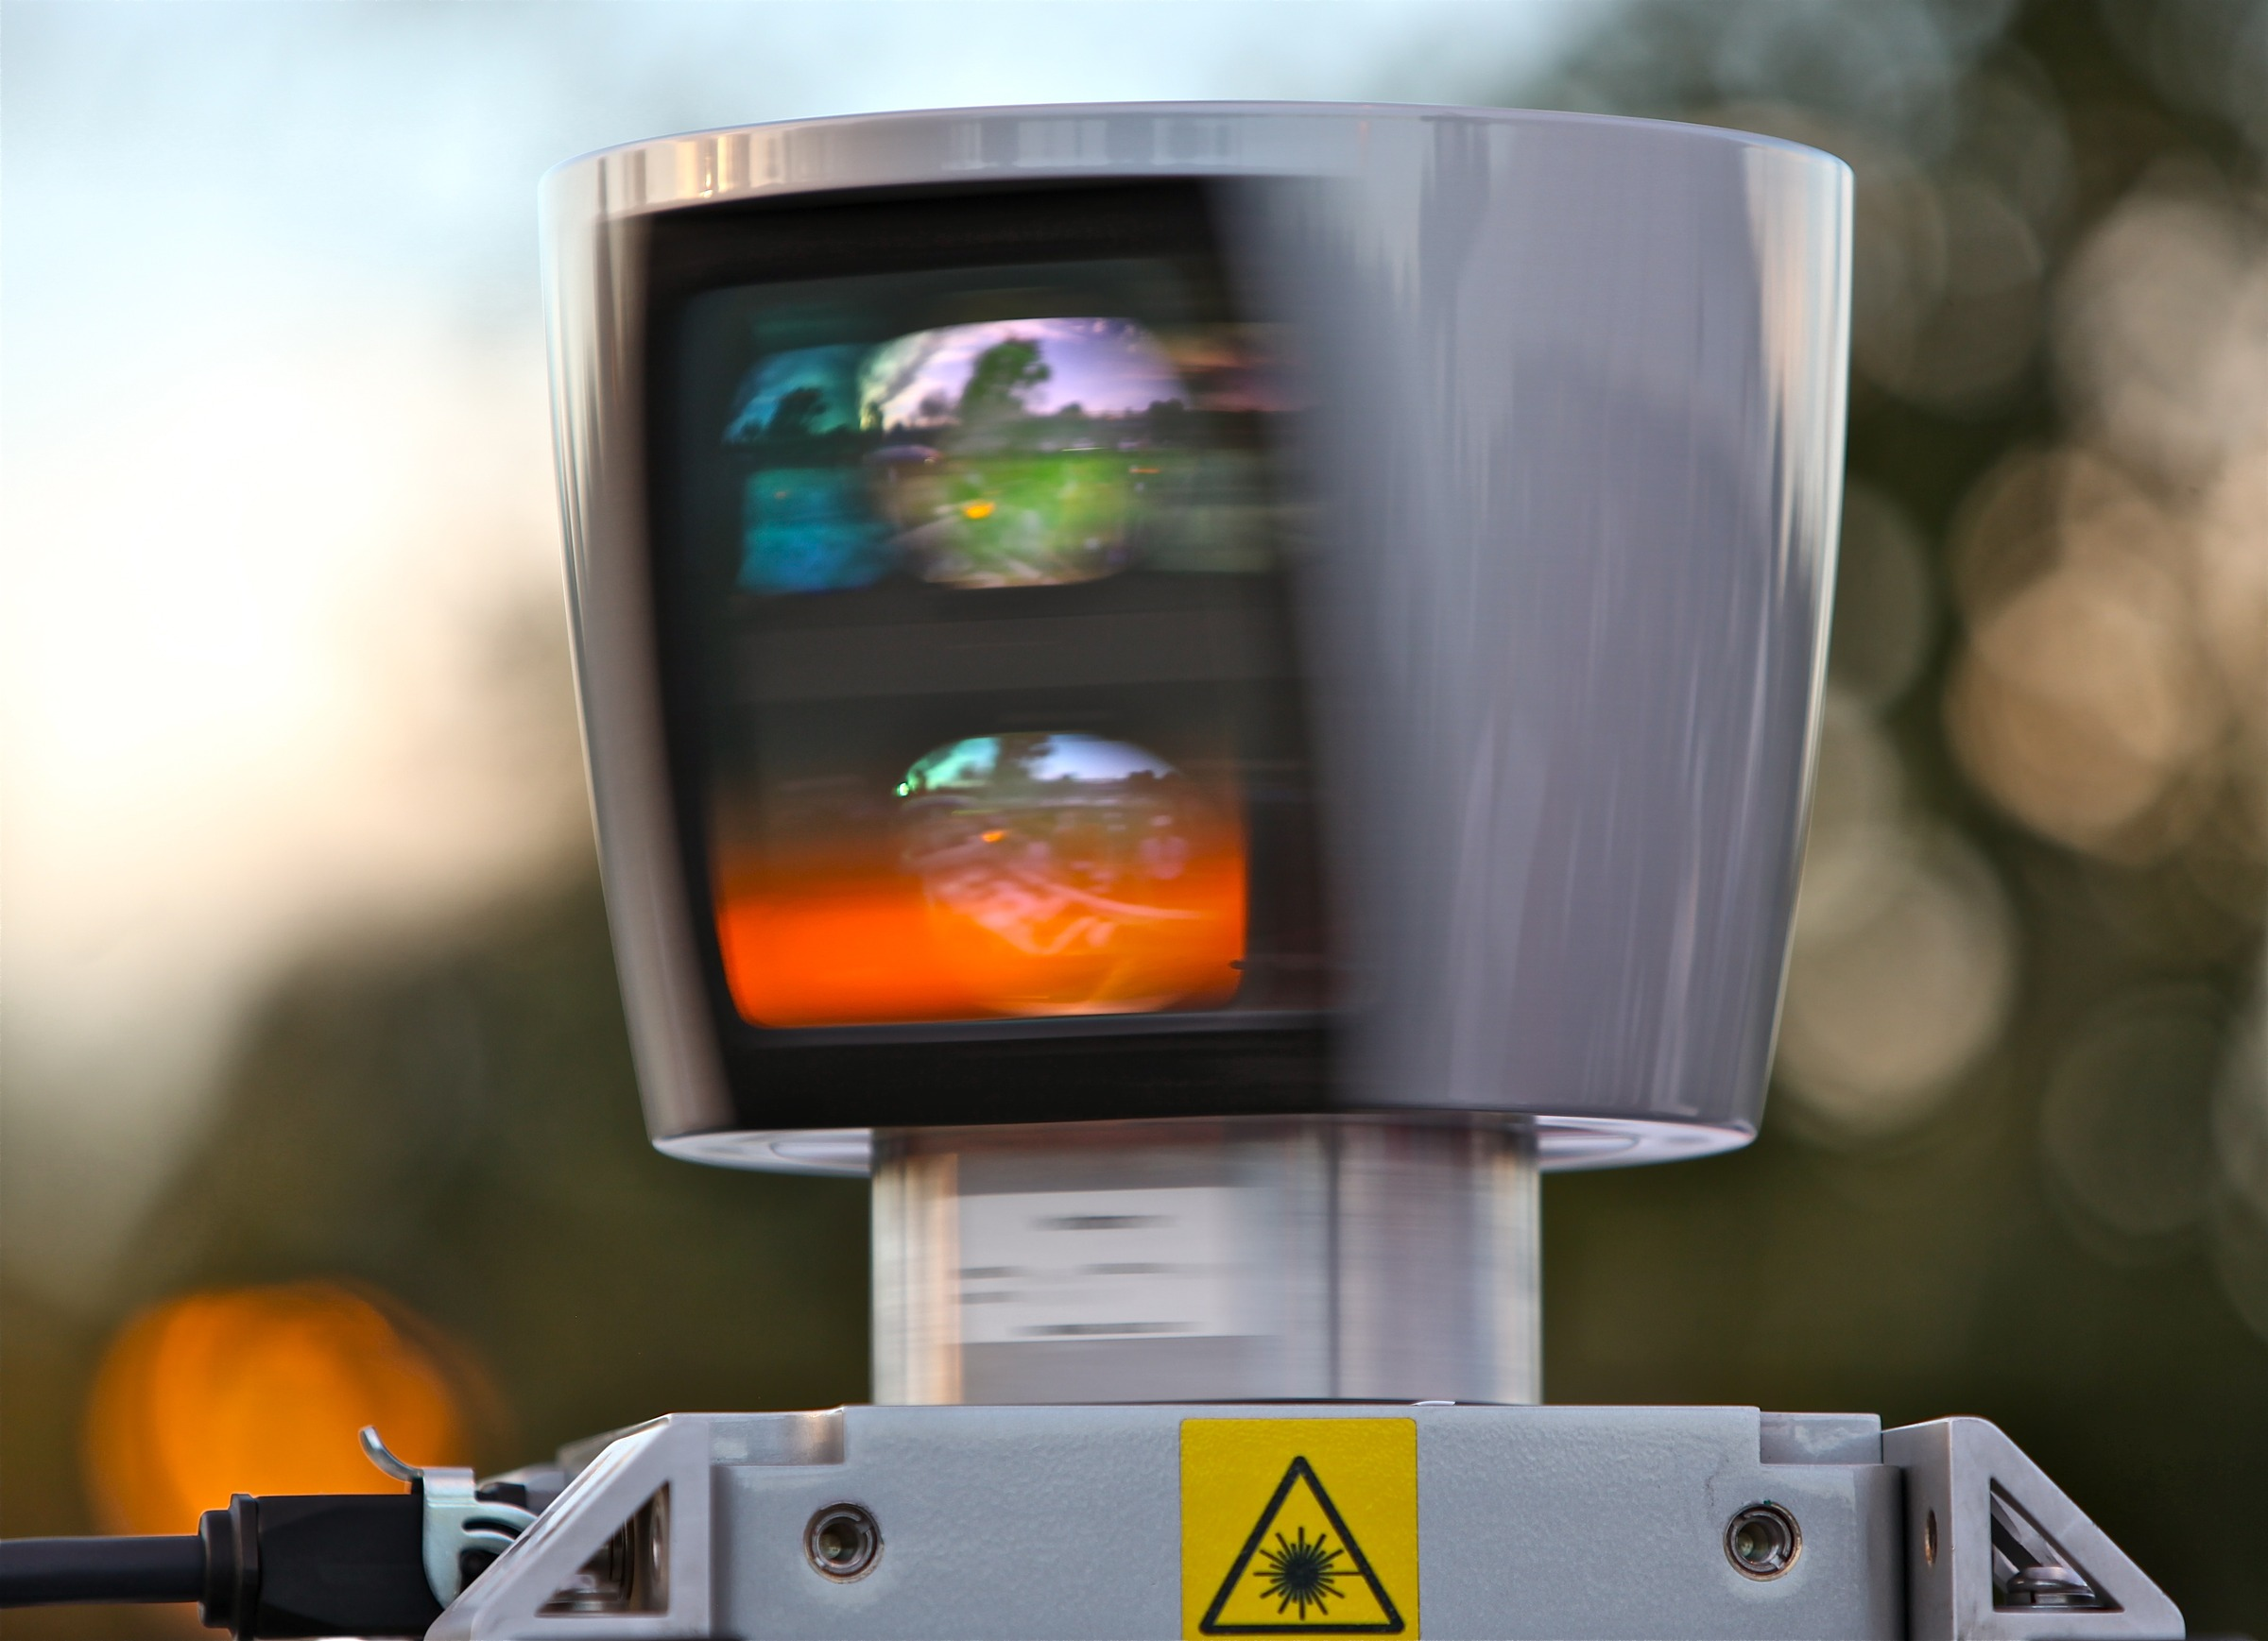
\includegraphics[width=0.85\linewidth,height=\textheight,keepaspectratio]{chapters/01-boundary/figures/fig01_real_lidar_sensor_rack.jpg}

}

\caption{\label{fig-01-sensor-rack}\textbf{Spinning Multi-Beam LiDAR
Sensor Hardware for Real-Time Perception.} Close-up photograph of the
64-beam spinning optical LiDAR sensor assembly (Velodyne HDL-64E)
mounted aboard an autonomous research testbed. In Physical AI,
high-bandwidth sensor streams (1.33 million points/second) must be
serialized over real-time interfaces (e.g., FPD-Link III, GMSL2,
Automotive Ethernet), synchronized via hardware timestamps, and
processed through neural perception backbones within strict end-to-end
latency budgets, because every millisecond of transport and compute
delay converts directly into unguided physical displacement. (Source:
Steve Jurvetson, CC BY 2.0).}

\end{figure}%

Understanding why Physical AI requires a distinct systems engineering
discipline requires contrasting its core properties against both
advisory digital machine learning and classical control theory. As
summarized in table~\ref{tbl-01-paradigm-comparison}, the three
paradigms are sorted from pure software isolation on the left, to pure
classical dynamics in the middle, to the unified physical AI synthesis
on the right.

\begin{longtable}[]{@{}
  >{\raggedright\arraybackslash}p{(\linewidth - 6\tabcolsep) * \real{0.2500}}
  >{\raggedright\arraybackslash}p{(\linewidth - 6\tabcolsep) * \real{0.2500}}
  >{\raggedright\arraybackslash}p{(\linewidth - 6\tabcolsep) * \real{0.2500}}
  >{\raggedright\arraybackslash}p{(\linewidth - 6\tabcolsep) * \real{0.2500}}@{}}
\caption{\textbf{Comparison Matrix of Computing Paradigms across the
Causal Boundary.} Systematic comparison of Advisory Digital Machine
Learning (left), Classical Robotics \& Control Theory (middle), and
Physical Artificial Intelligence (right) across operational substrate,
model formulation, feedback dynamics, execution cadence, actuation
authority, failure semantics, and safety certification
primitives.}\label{tbl-01-paradigm-comparison}\tabularnewline
\toprule\noalign{}
\begin{minipage}[b]{\linewidth}\raggedright
Architectural Dimension
\end{minipage} & \begin{minipage}[b]{\linewidth}\raggedright
Digital Machine Learning (Advisory)
\end{minipage} & \begin{minipage}[b]{\linewidth}\raggedright
Classical Robotics \& Control
\end{minipage} & \begin{minipage}[b]{\linewidth}\raggedright
Physical Artificial Intelligence (Closed-Loop)
\end{minipage} \\
\midrule\noalign{}
\endfirsthead
\toprule\noalign{}
\begin{minipage}[b]{\linewidth}\raggedright
Architectural Dimension
\end{minipage} & \begin{minipage}[b]{\linewidth}\raggedright
Digital Machine Learning (Advisory)
\end{minipage} & \begin{minipage}[b]{\linewidth}\raggedright
Classical Robotics \& Control
\end{minipage} & \begin{minipage}[b]{\linewidth}\raggedright
Physical Artificial Intelligence (Closed-Loop)
\end{minipage} \\
\midrule\noalign{}
\endhead
\bottomrule\noalign{}
\endlastfoot
\textbf{Operational Substrate} & Decoupled virtual memory buffers (GPU
VRAM, DRAM, web endpoints) & Continuous analog state space governed by
differential equations & Hybrid: high-dimensional neural representations
mapped to analog physical actuators \\
\textbf{Model Formulation} & High-capacity statistical approximators
(LLMs, ViTs, diffusion policies) & Analytically specified transfer
functions and deterministic state-space matrices & Foundation policies
paired with deterministic runtime safety filters \\
\textbf{Feedback Dynamics} & Exogenous and static; independent and
identically distributed samples & Continuous deterministic state
feedback with Gaussian sensor noise & Endogenous, non-stationary closed
loop; actions shape future observations \\
\textbf{Execution Cadence} & Throughput-optimized batching; soft or
unbounded latency budgets & Hard real-time single-rate loops on
microcontrollers (100--1000 Hz) & Asynchronous multi-rate cadences:
System 2 (1 Hz), System 1.5 (50 Hz), System 1 (1000 Hz) \\
\textbf{Actuation Authority} & Advisory; sandboxed APIs, display
buffers, or human-in-the-loop validation & Hardcoded feedback directly
driving power inverter timers and PWM registers & Decoupled
Proposal--Permission architecture; untrusted proposals gated by MCU
safety referee \\
\textbf{Failure Semantics} & Idempotent; call-stack unwind, database
rollback, or human alert dismissal & Actuator saturation or tracking
error within analytically bounded stability envelope & Irreversible
thermodynamic work, plastic deformation, kinetic collision, or stator
overheating \\
\textbf{Safety Assurance} & Offline statistical loss minimization on
validation splits & Formal mathematical stability proofs (Lyapunov
functions, gain/phase margins) & Layered runtime invariant enforcement,
forward-invariant barrier filters, and fault injection \\
\end{longtable}

\section{Three Machine Archetypes}\label{sec-boundary-1-3}

Once digital predictions cross the causal boundary into physical force,
they interact with physical machines of every conceivable shape and
scale. An autonomous delivery drone navigating turbulent wind gusts
seems to share nothing with a six-axis robotic arm assembling an
automotive transmission, and neither appears related to a containerized
battery management plant regulating liquid coolant. A practitioner or
student might wonder: how can a single systems engineering curriculum
possibly encompass such wildly diverse physical systems without
dissolving into a collection of bespoke, ad-hoc recipes?

The key is to look past cosmetic form factors and examine the underlying
physical conservation law that binds the machine. Beneath the surface
diversity of shapes, sizes, and applications, every embodied AI system
can be systematically categorized into one of three canonical physical
archetypes based on the physical quantity its actuators manipulate
(figure~\ref{fig-01-three-archetypes}): moving mass across space,
applying force through physical contact, or regulating continuous fluid
and thermal flows. By viewing physical AI through this three-archetype
lens, a systems architect can immediately determine which resource
budget is exhausted first during a software stall or model anomaly, and
design the real-time nervous system accordingly.

\subsection{Class 1: Mass-Dominated Mobility Systems (Moving Through
Space)}\label{class-1-mass-dominated-mobility-systems-moving-through-space}

Class 1 machines move mass across space, where execution is bound first
by momentum conservation and kinetic energy dissipation
(figure~\ref{fig-01-three-archetypes} a). In autonomous transport
platforms, quadruped robots navigating rugged terrain, mobile
manipulators, and aerial drones, the actuator bridge applies force to
translate or rotate a body with mass \(m\) at velocity \(v\). Because
kinetic energy \(E_k = \frac{1}{2}m v^2\) cannot be recalled once
delivered to the chassis, safety is measured as remaining spatial
clearance. When braking begins at maximum allowable deceleration
\(a_{\max}\), the physical floor for stopping distance follows the
fundamental kinematic relation:

\[d_{\text{stop}} = v \cdot t_{\text{lag}} + \frac{v^2}{2a_{\max}}\]

where \(t_{\text{lag}}\) is the total sense-to-actuation transport and
inference delay. In a mass-moving system, computational latency converts
directly into unguided spatial displacement
(\(v \cdot t_{\text{lag}}\)), while braking distance scales
quadratically with velocity (\(v^2 / 2a_{\max}\)). The first boundary
breached during a software stall or model misclassification is the
physical distance to an external obstacle.

\subsection{Class 2: Contact-Dominated Manipulation Systems (Applying
Contact
Force)}\label{class-2-contact-dominated-manipulation-systems-applying-contact-force}

Class 2 machines apply mechanical force through contact, where the
primary binding limit is actuator torque saturation, current loop
bandwidth, and structural stiffness
(figure~\ref{fig-01-three-archetypes} b). In articulated manipulators,
precision assembly fixtures, and robot learning workcells executing
contact-rich insertion and grasping, the end-effector interacts directly
with a rigid or compliant workpiece. Unlike a mobile platform operating
in open space, an arm in contact with a surface cannot resolve an
unexpected displacement command by rolling forward. When an actuator
commands position into a rigid boundary, displacement is constrained and
the interaction is governed by mechanical impedance. By Hooke's law, the
contact force generated by a spatial penetration error \(\Delta x\)
against an environment of stiffness \(k\) is
\(F = k \Delta x\).\sidenote{\footnotesize Rigid contact obeys Signorini-Coulomb
  complementarity (\(0 \le \delta \perp F_N \ge 0\)). Real-time stacks
  approximate compliance via Kelvin-Voigt models to prevent force loop
  divergence.}

Because contact stiffness in metal and tooling fixtures is extremely
high (\(k \ge 10^5\text{ N/m}\)), small geometric trajectory deviations
convert into massive contact forces within milliseconds. If the nervous
system fails to clamp motor current within sub-millisecond response
windows, the motor drives the transmission past its mechanical yield
stress. For example, a tooling tip moving at just \(0.20\text{ m/s}\)
that encounters a stiff workcell fixture will accumulate
\(30\text{ mm}\) of uncorrected displacement during a \(150\text{ ms}\)
software stall---generating thousands of Newtons of force that instantly
shears precision gear teeth. The critical floor in contact systems is
not stopping distance, but the time rate of force rise relative to
actuator current loop bandwidth and structural yield stress.

\subsection{Class 3: Flow-Dominated Process and Energy Systems
(Regulating Energy and Fluid
Flows)}\label{class-3-flow-dominated-process-and-energy-systems-regulating-energy-and-fluid-flows}

Beyond moving linkages and rigid contacts, Class 3 machines regulate
continuous fluid, thermal, or electrical power flows---a domain that
serves both as dedicated process plants and as the foundational
electrical and thermal substrate underlying all high-performance mobile
and manipulation systems (figure~\ref{fig-01-three-archetypes} c). In
grid-scale battery storage facilities, datacenter liquid cooling loops,
and grid-tied power inverters managing renewable generation, actuators
manipulate coolant pumps, flow valves, and high-frequency power
semiconductors rather than mechanical joints. The state of the system is
governed by mass transport, thermal capacitance, and energy balance
rather than kinematic positions. When a coolant valve or pump stalls,
accumulated heat drives rapid temperature excursions toward chemical
decomposition thresholds. Similarly, a grid-tied inverter operating on a
\(60\text{ Hz}\) utility network faces an electrical phase cycle of
\(16.6\text{ ms}\) (half-cycle zero crossing of \(8.33\text{ ms}\)),
where an unhandled scheduling delay creates alternating-current phase
angle errors that drive destructive surge currents through substation
transformers. The deadline in flow architectures is set by thermal
capacitance, transport delay, and grid phase timing, defining physical
budgets where accumulated energy cannot be quickly reversed once
started.

\subsection{The Integrative Capstone: Multi-Class Embodiments and
Humanoid
Robotics}\label{the-integrative-capstone-multi-class-embodiments-and-humanoid-robotics}

A central question for physical AI systems architects is: \emph{Where do
complex general-purpose embodiments, such as humanoid robots, fit into
this tri-archetype framework?}

A humanoid robot is not a disjoint fourth archetype. Rather, it
represents the \textbf{Integrative Capstone Embodiment}---the ultimate
cyber-physical convergence where all three canonical physical classes
operate and contend simultaneously on a single, tightly constrained
mobile chassis:

\begin{enumerate}
\def\labelenumi{\arabic{enumi}.}
\tightlist
\item
  \textbf{Class 1 Dynamics in Locomotion:} Underactuated bipedal
  balancing, dynamic footstep placement, momentum conservation
  (\(m\mathbf{v}\)), and ground contact slip during walking and stair
  climbing require continuous spatial clearance and kinetic energy
  management.
\item
  \textbf{Class 2 Dynamics in Manipulation:} High-DOF bimanual arms and
  dexterous tactile hands interacting with rigid workpieces, opening
  doors, and grasping tools generate instantaneous contact wrenches
  (\(\mathbf{F} = k \Delta \mathbf{x}\)) bounded by gearbox yield stress
  and joint impedance control bandwidth.
\item
  \textbf{Class 3 Dynamics in Actuation \& Power Delivery:} Driving 20
  to 50 high-torque actuators simultaneously from a single onboard DC
  battery pack pushes inverter thermal dissipation (\(I^2 R\)) to its
  limits and creates severe inductive power-rail voltage droop
  (\(L \frac{dI}{dt}\)) during simultaneous leg shock absorption and
  heavy arm lifting.
\end{enumerate}

While a single-class machine (such as a wheeled AMR or a fixed
industrial arm) isolates its physical budget to a single dominant
conservation law, a humanoid robot forces the systems architect to
manage \textbf{cross-class coupled contention}. When a bipedal robot
catches a falling heavy object, the contact wrench (Class 2) shifts its
center of mass, requiring an instantaneous balancing recovery step
(Class 1) that draws peak phase currents threatening to collapse the
electrical bus and overheat the knee actuators (Class 3). Throughout
this book, we will use individual archetypes to isolate specific
architectural principles in depth, while using humanoid robotics as the
capstone testbed where all physical constraints collide.

\begin{figure}[t]

\centering{

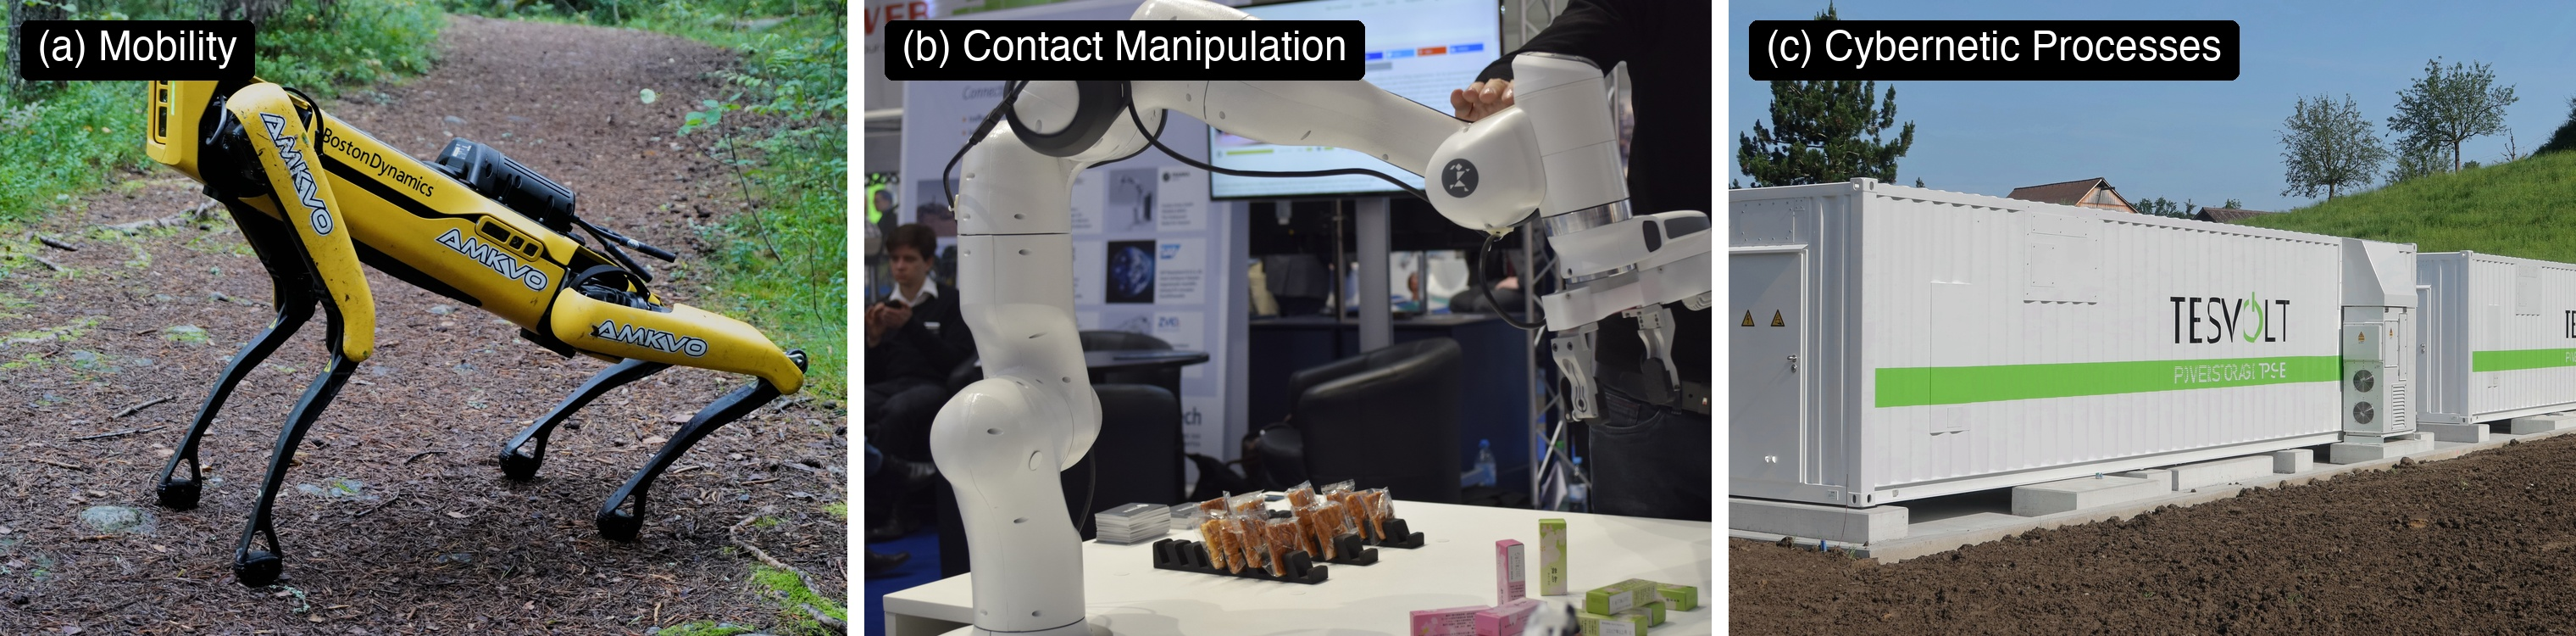
\includegraphics[width=1\linewidth,height=\textheight,keepaspectratio]{chapters/01-boundary/figures/fig01_three_archetypes.jpg}

}

\caption{\label{fig-01-three-archetypes}\textbf{The Three Canonical
Machine Archetypes of Physical AI.} (a) Mass-dominated mobility systems
(such as the Boston Dynamics Spot quadruped robot navigating rugged
outdoor terrain) bound first by momentum, kinetic energy dissipation,
and spatial clearance. (b) Contact-dominated manipulation systems (such
as the Franka Emika Panda articulated arm) bound first by contact
impedance, joint torque saturation, and structural yield stress. (c)
Flow-dominated process and thermal plants (such as containerized
grid-scale battery storage systems) bound first by lumped thermal
capacity, transport lag, and electrical phase timing. Complex
embodiments like humanoid robots serve as the integrative capstone
uniting all three classes on a single chassis. (Sources: Wikimedia
Commons, CC BY-SA 4.0).}

\end{figure}%

For any physical AI system, engineering the nervous system begins by
determining which physical budget is exhausted first during a failure.
In software systems, resource constraints center on processor cycles,
memory allocation, and network bandwidth. In physical systems, the
systems architect must identify whether spatial clearance, structural
stress, or heat dissipation creates the critical timing deadline. In a
high-speed vehicle or quadruped, spatial clearance fails within
fractions of a second while motor winding temperatures remain safely
below thermal limits. In an assembly press, mechanical stress exceeds
the yield point of structural members within tens of milliseconds long
before the chassis moves perceptibly or heats up. In a chemical reactor
or battery pack, mechanical stress is negligible, but accumulated
thermal energy breaches safe operational envelopes over several seconds.
The shortest time to failure across these three domains defines the
deterministic execution deadline that the nervous system must meet.

Yet understanding that a machine belongs to one of these three physical
archetypes does not automatically mean it requires the full systems
discipline of Physical AI. A classical hydraulic press or a
deterministic PID drone autopilot manipulates mass and contact force,
but operates entirely within classical control theory. To determine when
a machine crosses into Physical AI, we must establish a rigorous
diagnostic scope test.

\section{The Physical AI Scope Test}\label{sec-boundary-1-4}

Before designing or deploying an embodied architecture, a system
architect or practitioner must establish whether a machine actually
requires the full systems engineering discipline of Physical AI. Without
a rigorous scope boundary, engineering teams make two symmetric
mistakes: they over-engineer classical deterministic machines with
bloated neural models where closed-form PID control is provably optimal,
or they dangerously under-engineer stochastic neural models by granting
them unverified motor authority in safety-critical physical loops.

The scope of Physical AI is defined by the simultaneous intersection of
three structural criteria (figure~\ref{fig-01-scope-venn}):

\begin{enumerate}
\def\labelenumi{\arabic{enumi}.}
\tightlist
\item
  \textbf{Learned Statistical Model (Unspecifiable Policy):} The system
  relies on a policy, perception encoder, or world model acquired from
  data (e.g., neural networks, foundation models, diffusion policies)
  whose transfer function cannot be written in closed-form analytical
  equations and whose worst-case outputs cannot be mathematically
  bounded offline.
\item
  \textbf{Consequential Physical Feedback:} Actuator actions alter the
  material state of the physical environment, endogenously determining
  what the sensors observe next under the governing laws of classical
  mechanics, thermodynamics, or electromagnetism.
\item
  \textbf{Delegated Physical Authority (Direct Actuator Write):}
  Automated software routines write directly to hardware actuator
  registers without synchronous human approval in the control loop,
  operating within the temporal window where delay or error converts
  directly into irreversible physical momentum.
\end{enumerate}

\begin{figure}[t]

\centering{


\includegraphics[width=0.9\linewidth,height=\textheight,keepaspectratio]{index_files/mediabag/chapters/01-boundary/figures/fig01_scope_venn.pdf}

}

\caption{\label{fig-01-scope-venn}\textbf{The Physical AI Scope Test.}
Physical AI exists strictly at the three-way intersection of learned
models (unspecifiable policies), consequential physical feedback
(actions govern future sensory observations under mechanics and
thermodynamics), and delegated physical authority (automated register
writes without synchronous human intervention). Systems satisfying
exactly two criteria define adjacent engineering fields: Advisory
Decision Support (no physical authority), Classical Control Theory
(analytical transfer functions with Lyapunov certificates), and Digital
Autonomous Systems (transactional databases with idempotency and
rollback). The shared autonomy reflex gap marks the operational boundary
where human neuromuscular reflex latency (\(150\text{--}250\text{ ms}\))
delegates transient authority to the learned model.}

\end{figure}%

A closed feedback loop is necessary for physical interaction, but
feedback alone does not place a machine in this domain. Classical
proportional-integral-derivative controllers run at \(1000\text{ Hz}\)
across aerospace and industrial automation, regulating valve positions
and motor torques through tight sensory feedback. Their feedback loops
are continuous and physical, but their control laws are specified
entirely by fixed mathematical formulas whose stability bounds can be
proven analytically from transfer functions. They hold physical
authority and experience physical feedback, but they lack a learned
model. Conversely, high-frequency algorithmic trading engines execute
automated market orders under learned predictive models within
microseconds. They combine learned policies with delegated transactional
authority, but the feedback they receive is purely digital and
informational. When an order executes, it alters an electronic order
book rather than momentum, friction, or thermal energy. An unhandled
stall in algorithmic trading costs financial capital, but it does not
cause an inertia-driven collision with a structural fixture.

A learned model is equally insufficient on its own to define the field.
Modern engineering workflows frequently deploy deep neural networks to
optimize robot trajectories offline or inspect manufactured parts on
assembly lines. An offline neural trajectory optimizer may compute
time-optimal paths for a six-axis robotic manipulator over several
seconds of cluster compute, but if that trajectory is verified by an
engineer or executed through a classical deterministic controller with
hard-coded envelope stops, the learned model holds no delegated physical
authority over the plant. Similarly, a convolutional neural network
monitoring an assembly line may classify surface defects at
\(60\text{ frames/s}\). If the classification output merely logs an
entry in a database or flags a display for a human operator, the model
operates outside the causal loop. A false negative or an inference
timeout produces a corrupted record, but it cannot directly command an
actuator to over-torque a mechanical joint.

Systems that satisfy exactly two criteria demonstrate where the
structural boundary lies. A real-time driver drowsiness monitor uses a
learned computer vision model to track eyelid movement and vehicle lane
position, receiving continuous physical feedback from the vehicle state.
Yet it lacks delegated physical authority because its only output is an
auditory warning chime. If the vision model fails completely during an
inference stall, the speaker emits no sound, but the steering rack and
brake calipers remain under human control. An analog bimetallic
thermostat possesses delegated physical authority over a gas furnace
valve and operates in continuous feedback with the thermal mass of a
building, but its transfer function is a fixed thermodynamic property of
two bonded metals rather than a learned representation. An automated
trading bot possesses both a learned policy and delegated execution
authority, but its actions propagate through network packets and
databases without interacting with the physical laws of mass and motion.

The most demanding edge cases occur in shared autonomy, where physical
authority is divided dynamically between a human operator and a learned
model. In robotic surgery or advanced driver assistance, a human
operator provides continuous steering or tool guidance while a learned
policy injects corrections to filter hand tremors, avoid anatomical
boundaries, or compensate for vehicle slip. These architectures satisfy
both the learned component and physical feedback criteria. Whether they
fall within the scope of Physical AI depends strictly on the temporal
authority granted to the model. If the learned policy can command even
\(2.0\text{ N}\) of force or adjust steering angle without requiring
human confirmation within the \(200\text{ ms}\) threshold of human
reflex latency, the model possesses delegated physical authority. During
that \(200\text{ ms}\) window, an erroneous model output or a delayed
inference packet acts on the physical world before the operator can
intercede.

Evaluating an ambiguous machine requires a three-step decision rubric
that tests each criterion independently
(table~\ref{tbl-01-scope-matrix}). The first test determines whether the
system contains a policy component whose mapping is learned from data
rather than specified analytically in closed form. If it does not, the
machine belongs to classical control theory. The second test determines
whether actuator commands alter a physical plant such that subsequent
sensor observations are governed by mechanics, thermodynamics, or fluid
dynamics. If they do not, the machine is a digital machine learning
system. The third test determines whether the learned component writes
commands to physical actuators without a human supervisor or an
independent deterministic barrier capable of vetoing the action before
physical momentum accumulates. If it does not, the machine is an offline
decision-support tool. When all three tests pass, the system operates as
Physical AI, and its engineering must be governed by the laws of the
causal boundary.

\begin{longtable}[]{@{}
  >{\raggedright\arraybackslash}p{(\linewidth - 10\tabcolsep) * \real{0.1667}}
  >{\raggedright\arraybackslash}p{(\linewidth - 10\tabcolsep) * \real{0.1667}}
  >{\raggedright\arraybackslash}p{(\linewidth - 10\tabcolsep) * \real{0.1667}}
  >{\raggedright\arraybackslash}p{(\linewidth - 10\tabcolsep) * \real{0.1667}}
  >{\raggedright\arraybackslash}p{(\linewidth - 10\tabcolsep) * \real{0.1667}}
  >{\raggedright\arraybackslash}p{(\linewidth - 10\tabcolsep) * \real{0.1667}}@{}}
\caption{\textbf{The Physical AI Scope Test Decision Matrix.} Systematic
evaluation of representative engineering systems across the three joint
criteria (Learned Model, Consequential Physical Feedback, and Delegated
Physical Authority), establishing the governing engineering discipline,
limiting physical factors, and primary failure modes for each
candidate.}\label{tbl-01-scope-matrix}\tabularnewline
\toprule\noalign{}
\begin{minipage}[b]{\linewidth}\raggedright
System Candidate / Case
\end{minipage} & \begin{minipage}[b]{\linewidth}\raggedright
Criterion 1: Learned Model (Unspecifiable Policy)
\end{minipage} & \begin{minipage}[b]{\linewidth}\raggedright
Criterion 2: Consequential Physical Feedback
\end{minipage} & \begin{minipage}[b]{\linewidth}\raggedright
Criterion 3: Delegated Physical Authority (Direct Actuator Write)
\end{minipage} & \begin{minipage}[b]{\linewidth}\raggedright
Scope Classification \& Discipline
\end{minipage} & \begin{minipage}[b]{\linewidth}\raggedright
Limiting Physics \& Critical Failure Mode
\end{minipage} \\
\midrule\noalign{}
\endfirsthead
\toprule\noalign{}
\begin{minipage}[b]{\linewidth}\raggedright
System Candidate / Case
\end{minipage} & \begin{minipage}[b]{\linewidth}\raggedright
Criterion 1: Learned Model (Unspecifiable Policy)
\end{minipage} & \begin{minipage}[b]{\linewidth}\raggedright
Criterion 2: Consequential Physical Feedback
\end{minipage} & \begin{minipage}[b]{\linewidth}\raggedright
Criterion 3: Delegated Physical Authority (Direct Actuator Write)
\end{minipage} & \begin{minipage}[b]{\linewidth}\raggedright
Scope Classification \& Discipline
\end{minipage} & \begin{minipage}[b]{\linewidth}\raggedright
Limiting Physics \& Critical Failure Mode
\end{minipage} \\
\midrule\noalign{}
\endhead
\bottomrule\noalign{}
\endlastfoot
\textbf{Autonomous Warehouse AMR (Class 1)} & \textbf{Yes} (Learned
navigation policy / costmap) & \textbf{Yes} (Kinetic momentum, chassis
inertia, and wheel traction) & \textbf{Yes} (Direct motor drive packets
without human in loop) & \textbf{Physical AI} & Kinetic impact; traction
slip and odometry loss \\
\textbf{Articulated Contact Manipulator (Class 2)} & \textbf{Yes}
(Diffusion action chunking for assembly) & \textbf{Yes} (Mechanical
contact impedance and reaction forces) & \textbf{Yes} (Direct joint
torque and velocity register writes) & \textbf{Physical AI} & Structural
yield stress exceedance; gearbox tooth shear \\
\textbf{High-Speed Drone Classical Autopilot} & \textbf{No}
(Analytically tuned 1000 Hz PID / cascaded loop) & \textbf{Yes}
(Aerodynamic lift, drag, and gyroscopic dynamics) & \textbf{Yes} (Direct
PWM motor speed control) & \textbf{Classical Control Theory} & Control
margin erosion; rotor thrust saturation \\
\textbf{High-Frequency Market Maker} & \textbf{Yes} (Deep transformer
sequence predictor) & \textbf{No} (Digital order-book state; memory and
network queues) & \textbf{Yes} (Automated limit order execution over 10
GbE) & \textbf{Digital Machine Learning / FinTech} & Financial capital
loss; market flash crash (idempotent rollback) \\
\textbf{Advisory Driver Drowsiness Monitor} & \textbf{Yes} (Facial
landmark vision network) & \textbf{Yes} (Vehicle kinematics and driver
physiology) & \textbf{No} (Auditory warning buzzer and dashboard LED
only) & \textbf{Advisory Decision Support} & Human perception-reaction
latency; zero physical authority \\
\textbf{Offline Trajectory Optimizer} & \textbf{Yes} (Deep neural
network for time-optimal path search) & \textbf{No} (Static CAD workcell
model; offline batch execution) & \textbf{No} (Motion plan verified and
loaded via human engineer) & \textbf{Offline Optimization Tool} &
Numerical non-convergence; zero direct runtime plant coupling \\
\textbf{Shared-Autonomy Surgical Assist} & \textbf{Yes} (Learned haptic
tremor filter / virtual fixtures) & \textbf{Yes} (Anatomical tissue
compliance and reaction forces) & \textbf{Conditional} (Model injects
forces within human reflex window) & \textbf{Borderline / Shared
Physical AI} & Human neuromuscular reflex latency vs.~tool force rise
rate \\
\end{longtable}

\section{The Four Pillars of an Embodied Agent}\label{sec-boundary-1-5}

Before exploring how physical systems fail or examining the silicon
circuits that control them, we must map the complete anatomical
landscape of an embodied machine. Every physical AI system---whether a
humanoid biped, an autonomous tractor, or an automated surgical
console---is composed of four fundamental architectural pillars that
operate across distinct physical timescales:

\begin{enumerate}
\def\labelenumi{\arabic{enumi}.}
\tightlist
\item
  \textbf{Pillar 1: The Dynamical Body (Layer 1):} The physical plant
  itself. Comprising mechanical linkages, structural mass, gear
  transmissions, motor windings, power electronic inverters, and battery
  packs. The body does not obey software abstractions, but rather the
  governing conservation laws of classical mechanics, thermodynamics,
  and electromagnetism. It accumulates fatigue, dissipates resistive
  Joule heat (\(I^2 R\)), and resists instantaneous acceleration through
  reflected rotor inertia (\(N^2 J\)).
\item
  \textbf{Pillar 2: The Cognitive Brain (Layer 3):} The high-capacity
  learned intelligence. Comprising multi-modal vision-language-action
  (VLA) foundation models, diffusion policies, and semantic world models
  running on high-performance compute accelerators (GPUs, NPUs). The
  brain provides open-vocabulary generalization, spatial scene
  understanding, and long-horizon affordance reasoning. Its competence
  arises from high-dimensional statistical approximation across massive
  datasets, meaning it is fundamentally stochastic, non-deterministic,
  and prone to out-of-distribution hallucinations.
\item
  \textbf{Pillar 3: The Real-Time Nervous System (Layer 2):} The
  deterministic cyber-physical bridge. Comprising hard real-time
  microcontrollers (bare-metal MCUs), deterministic fieldbus networks
  (CAN-FD, EtherCAT, TSN Ethernet), and lock-free shared memory fabrics.
  The nervous system enforces sub-millisecond execution deadlines
  (\(1000\text{ Hz}\)), guarantees microsecond clock synchronization,
  evaluates candidate commands, and retains exclusive physical authority
  over actuator registers.
\item
  \textbf{Pillar 4: The Governance Envelope (Layer 4):} The formal
  safety, verification, and certification harness. Comprising
  forward-invariant safety monitors (Control Barrier Functions),
  decaying cryptographic operating leases, cross-layer hardware fault
  injection, and auditable Claim-Argument-Evidence (CAE) safety cases
  that qualify the complete machine for deployment.
\end{enumerate}

These four pillars form an integrated physical container. The Cognitive
Brain (Pillar 2) generates high-level intentions and proposed action
trajectories; the Real-Time Nervous System (Pillar 3) evaluates those
proposals against the physical constraints of the Dynamical Body (Pillar
1); and the Governance Envelope (Pillar 4) bounds the operational
envelope and provides formal assurance.

When any one of these four pillars is missing or compromised, the causal
boundary breaks. To see this catastrophic failure mode in forensic
detail, we examine one of the most famous real-world failures in
autonomous systems history.

\section{Anatomy of a Crash: When the Boundary
Fails}\label{sec-boundary-1-6}

To understand why the boundary conditions of Physical AI are not mere
theoretical classifications, but life-critical systems requirements, we
must examine what happens when an embodied machine violates them. When a
high-capacity learned model is granted unverified motor authority over
physical mass, software failure does not remain behind glass---it
converts into kinetic destruction. A physical crash in an autonomous
machine is rarely caused by an inaccurate prediction alone, but by the
absence of an architectural mechanism with the authority to refuse one.

\subsection{The 2018 Tempe Autonomous
Collision}\label{the-2018-tempe-autonomous-collision}

On a clear night in March 2018, an automated test vehicle---a modified
Volvo XC90 SUV operating Uber Advanced Technologies Group's
developmental Automated Driving System (ADS)---was traveling at
forty-three miles per hour (\(v_0 = 19.2\text{ m/s}\), mass
\(m \approx 2100\text{ kg}\)) along a public multi-lane roadway in
Tempe, Arizona (\citeproc{ref-ntsb2019uber}{National Transportation
Safety Board 2019})\sidenote{\footnotesize NTSB Highway Accident Report NTSB/HAR-19/03
  (2019). The investigation established that semantic classification
  toggling repeatedly reset tracking histories and suppressed emergency
  braking for \(1.2\text{ s}\), while factory autonomous emergency
  braking was disabled to prevent diagnostic bus conflicts with the
  prototype software stack.}. With a total kinetic energy of:

\[E_k = \frac{1}{2} m v_0^2 = \frac{1}{2}(2100\text{ kg})(19.2\text{ m/s})^2 \approx 387\text{ kJ}\]

the moving vehicle struck and fatally injured a pedestrian pushing a
bicycle across the asphalt.

The vehicle was equipped with an expansive, state-of-the-art physical
sensor suite (figure~\ref{fig-01-tempe-vehicle}): a roof-mounted 64-beam
Velodyne LiDAR (360° azimuth, \(> 100\text{ m}\) range), ten optical
cameras, and eight medium- and long-range radar units. At timestamp
\(T - 5.6\text{ s}\), while the vehicle was still \(82.0\text{ m}\)
away, the primary LiDAR and radar sensors established positive contact
with the obstacle, initializing a dynamic track in host computer memory.

\subsection{Perception Toggling and State
Erasure}\label{perception-toggling-and-state-erasure}

Despite continuous sensor contact over more than five seconds, the
vehicle failed to brake. Between \(T - 4.4\text{ s}\) and
\(T - 1.2\text{ s}\), the stochastic neural perception classifier
repeatedly toggled its semantic classification label between an
\emph{unknown vehicle}, a \emph{bicycle}, and an \emph{unclassified
static obstacle}.

Because the software tracking architecture associated Kalman filter
state estimators with discrete semantic categories, each classification
label switch caused the runtime to discard the existing kinematic track
and re-initialize a new filter instance with an assumed velocity vector
of zero. As a direct consequence of this classification instability, the
downstream trajectory planner never accumulated persistent evidence of
an imminent collision course.

\subsection{Latency Suppression and Kinematic
Depletion}\label{latency-suppression-and-kinematic-depletion}

At \(T - 1.2\text{ s}\), the software finally consolidated the track but
triggered an internal \(1.2\text{ s}\) ``suppression delay''---a
software counter designed by developers to prevent false-positive
emergency braking alarms from disrupting passenger comfort.

During this suppression window, the vehicle traversed an unguided
displacement of:

\[d_{\text{lag}} = v_0 \cdot t_{\text{suppress}} = (19.2\text{ m/s}) \times (1.2\text{ s}) \approx 23.0\text{ m}\]

When the planner finally completed the suppression window and requested
emergency braking at \(T - 0.2\text{ s}\), the remaining physical
clearance had collapsed to just \(3.8\text{ m}\). Bringing a
\(2100\text{ kg}\) vehicle to a complete halt on dry asphalt (assuming a
maximum deceleration \(a_{\max} \approx 8.0\text{ m/s}^2\)) requires a
physical braking distance of:

\[d_{\text{brake}} = \frac{v_0^2}{2 a_{\max}} = \frac{(19.2\text{ m/s})^2}{2 \times 8.0\text{ m/s}^2} \approx 23.0\text{ m}\]

Total stopping distance required at \(T - 1.2\text{ s}\) exceeded
\(d_{\text{stop}} = d_{\text{lag}} + d_{\text{brake}} = 23.0\text{ m} + 23.0\text{ m} = 46.0\text{ m}\).
Because available clearance had eroded to \(3.8\text{ m}\), kinetic
collision at full cruising speed was mathematically sealed two full
seconds before impact.

\begin{figure}[t]

\centering{

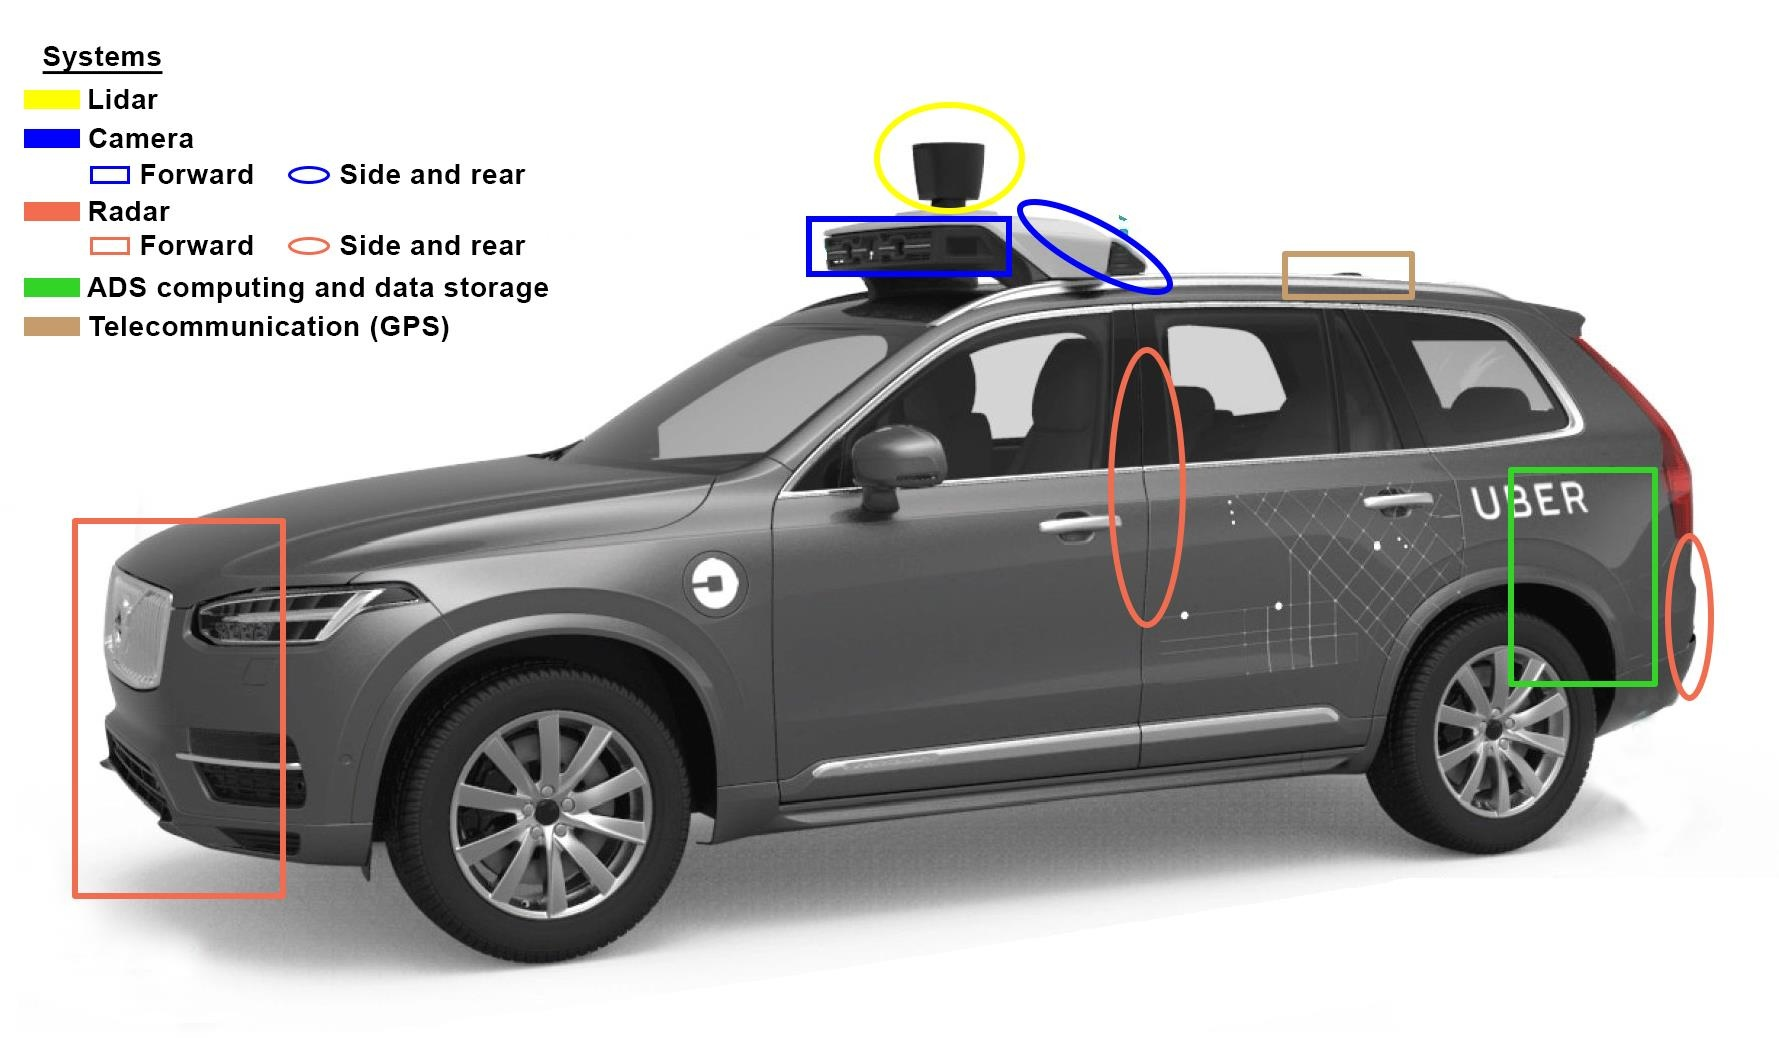
\includegraphics[width=0.95\linewidth,height=\textheight,keepaspectratio]{chapters/01-boundary/figures/fig01_real_ntsb_tempe_vehicle.jpg}

}

\caption{\label{fig-01-tempe-vehicle}\textbf{Autonomous Test Vehicle
Sensor Configuration from NTSB Collision Investigation.} The modified
2017 Volvo XC90 sport utility vehicle operating Uber ATG's developmental
Automated Driving System (ADS) during the March 2018 fatal collision in
Tempe, Arizona. The physical sensor suite comprised a roof-mounted
64-beam Velodyne LiDAR (360° azimuth, \textgreater100 m range), a
10-camera optical sensing suite including forward-facing stereo and
wide-angle cameras, and eight medium- and long-range radar units
providing 360° perimeter coverage. Despite continuous sensor contact
starting at 82 meters (\(T-5.6\text{ s}\)), classification instability
in the perception pipeline and an unverified 1.2-second suppression
delay prevented the planner from requesting braking until 0.2 seconds
before impact. (Source: NTSB Highway Accident Report NTSB/HAR-19/03
(\citeproc{ref-ntsb2019uber}{National Transportation Safety Board
2019}), Public Domain).}

\end{figure}%

\protect\phantomsection\label{callout-autopsyux2a-1.5}
\begin{fbxSimple}{callout-autopsy}{Incident Autopsy:}{The Missing Safety Referee}
\phantomsection\label{callout-autopsy*-1.5}

\begin{itemize}
\tightlist
\item
  \textbf{System:} Developmental Automated Driving System (ADS) on a
  2017 Volvo XC90 SUV (\(2100\text{ kg}\), \(19.2\text{ m/s}\)) equipped
  with roof-mounted 64-beam LiDAR, radar, and optical cameras.
\item
  \textbf{Incident:} Struck and fatally injured a pedestrian pushing a
  bicycle across an urban roadway without executing emergency braking
  before impact.
\item
  \textbf{Telemetry Snapshot:} Sensor contact established at
  \(T - 5.6\text{ s}\) (\(82\text{ m}\)); classifier toggled across
  three semantic labels for \(3.2\text{ s}\); \(1.2\text{ s}\)
  false-alarm suppression delay expired at \(T - 0.2\text{ s}\)
  (\(3.8\text{ m}\) remaining clearance).
\item
  \textbf{Root Cause:} Semantic classification toggling caused the
  tracker to repeatedly discard kinematic state histories and
  re-initialize velocity estimators to zero, preventing the trajectory
  planner from recognizing an imminent collision.
\item
  \textbf{Architectural Flaw:} Complete absence of an isolated
  deterministic safety referee running on dedicated real-time silicon
  with the authority to evaluate geometric clearance invariants directly
  against raw sensor points.
\item
  \textbf{Provenance:} National Transportation Safety Board Accident
  Report NTSB/HAR-19/03 (2019).
\end{itemize}

\end{fbxSimple}

This investigation autopsy demonstrates why refining perception models
or expanding offline training datasets cannot compensate for an
architectural absence of authority boundaries. An open-world statistical
model will inevitably encounter out-of-distribution scenes, sensor
degradations, and transient classification oscillations. The Tempe
vehicle crashed not because its neural network was imperfect, but
because the autonomy architecture lacked an isolated nervous system
running on dedicated real-time silicon with the independent authority to
evaluate spatial clearance and execute an emergency stop. If a
deterministic safety enforcer had continuously checked the stopping
clearance invariant at the hardware floor, the machine would have
executed emergency braking at \(T - 2.5\text{ s}\), bringing the vehicle
to a controlled halt long before available clearance
collapsed.\sidenote{\footnotesize Safety-critical systems combine deterministic
  functional safety (ISO 26262 ASIL-D, IEC 61508 SIL-3) with autonomous
  system standards: ISO 21448 (SOTIF) governs perception hazards and
  out-of-distribution limits, while UL 4600 mandates goal-structured
  safety cases requiring guaranteed transitions to a Minimal Risk
  Condition (MRC) upon subsystem anomaly.}

The forensic breakdown of the Tempe crash reveals four universal bedrock
laws that govern all physical machines across the causal boundary.

\section{The Four Bedrock Laws}\label{sec-boundary-1-7}

Four bedrock laws govern every machine whose nervous system translates
compute cycles into physical action. Notice how these four laws map
symmetrically to the \textbf{Four Pillars of an Embodied Agent} and the
\textbf{Four Parts of this Textbook}:

\protect\phantomsection\label{callout-lawux2a-1.6}
\begin{fbxSimple}{callout-law}{Bedrock Law:}{1. Physical Causality and Irreversibility (The Body Law — Part I)}
\phantomsection\label{callout-law*-1.6}

Software state can be caught with an exception block, isolated in a
virtual container, or restored from a checkpoint. Physical actions
governed by mass, inertia, friction, and gravity are permanent and
irreversible. Every actuation permanently alters the physical
environment, dissipates energy, and alters all future sensory
observations endogenously.

\end{fbxSimple}

The first bedrock law is the thermodynamic irreversibility of physical
action. In a pure software system, an erroneous operation is reversed by
rolling back a database transaction, restoring a file from a snapshot,
or restarting a process with clean memory. In a physical machine, an
actuator converts electrical charge into kinetic energy, structural
strain, or fluid pressure. Once that energy crosses the causal boundary
into the environment, it cannot be recalled. When an erroneous command
accelerates a warehouse robot toward an obstacle, the kinetic energy
deposited into the chassis can only be counteracted by applying opposing
forces through friction brakes, which dissipates the energy as heat. If
an over-current command drives a six-axis manipulator into an assembly
jig, the mechanical stress exceeds the yield point of the metal within
milliseconds, permanently deforming the tooling. Software transactions
can be rolled back, but thermodynamic work cannot be undone.

\protect\phantomsection\label{callout-lawux2a-1.7}
\begin{fbxSimple}{callout-law}{Bedrock Law:}{2. Endogenous Data and Compounding Drift (The Policy Law — Part II)}
\phantomsection\label{callout-law*-1.7}

A physical agent shapes its own future data distribution. Naive
behavioral cloning on open-loop benchmarks suffers compounding covariate
drift (\(\mathcal{O}(T^2 \epsilon)\)) in closed-loop execution. An error
on step \(t\) creates an out-of-distribution observation at step
\(t+1\), causing policy confidence to collapse into mechanical
divergence.

\end{fbxSimple}

The second bedrock law governs how embodied policies learn and fail. In
traditional computer vision or natural language processing, data is
exogenous: whether a model correctly identifies an image has zero effect
on the distribution of subsequent images. In Physical AI, every torque
command rotates joints, shifts camera angles, and alters contact forces.
The data stream is endogenous---created entirely by the machine's own
past actions. A single erroneous inference drives the hardware into an
unvisited state where neural predictions exhibit higher variance,
compounding errors until the machine exceeds physical stability limits.

\protect\phantomsection\label{callout-lawux2a-1.8}
\begin{fbxSimple}{callout-law}{Bedrock Law:}{3. Proposal–Permission Privilege and Freshness (The Nervous System Law — Part III)}
\phantomsection\label{callout-law*-1.8}

No stochastic neural network may hold direct motor authority. Learned
models running on application processors are unprivileged proposal
services. Real-time physical permission belongs exclusively to dedicated
microcontrollers executing deterministic safety filters at 1000 Hz.
Latency is physical displacement; stale proposals older than their
freshness deadline must be discarded.

\end{fbxSimple}

The third bedrock law requires strict separation between proposal and
permission. The subsystem of the nervous system that generates complex,
goal-directed behavior operates by optimization over high-dimensional
learned representations. Because deep neural networks are
uninterpretable and produce erratic outputs under out-of-distribution
inputs, a learned policy must never hold direct write access to physical
actuator registers. The role of the learned model is strictly to propose
candidate trajectories. The authority to grant permission, clip commands
to safe physical envelopes, or reject the proposed action entirely must
belong to a separate, deterministic supervisory layer running on
isolated execution hardware.

\protect\phantomsection\label{callout-lawux2a-1.9}
\begin{fbxSimple}{callout-law}{Bedrock Law:}{4. Governed Authority and Defensible Release (The Governance Law — Part IV)}
\phantomsection\label{callout-law*-1.9}

Physical AI systems are never `generally safe'; operating authority is a
decaying lease strictly conditioned on bounded evidence. A cherry-picked
video demonstration is not evidence of safety; defensible release
requires cross-layer hardware fault injection, formal barrier
guarantees, and an auditable safety case.

\end{fbxSimple}

The fourth bedrock law dictates that deployment readiness cannot be
justified by empirical validation loss. In cloud computing, software
reliability is evaluated statistically: an engineer measures mean
accuracy, accepts an uptime target of \(99.9\%\), and resolves rare
corner-case crashes through automated restarts and rolling updates. In
physical AI, the tail of the error distribution manifests as mechanical
destruction. Safe operation cannot be certified by average-case
performance metrics gathered over finite training sets. It requires
formal, worst-case envelope bounds verified against the physical laws of
the plant, ensuring that even if the learned proposal violates safety
limits, the machine remains within guaranteed physical boundaries.

The four bedrock laws establish the physical constraints that govern
every machine. But of these four, the Law of Proposal--Permission
Privilege dictates how we must architect and physically build the
computer system. How do we take an untrusted, stochastic neural policy
and safely translate its high-level intelligence into physical motion on
real hardware?

\section{The Dual-Brain Architecture}\label{sec-boundary-1-8}

To safely bridge high-capacity learned policies and real-time physical
machines, the systems architect implements the
\textbf{Proposal--Permission Architecture} across heterogeneous silicon.
The system partitions compute into two physically separated execution
domains: an unprivileged application processor (Linux MPU or Edge NPU)
generating candidate action proposals at deliberative cadences
(\(10\text{--}50\text{ Hz}\)), paired with an isolated, zero-allocation
real-time microcontroller (bare-metal MCU) executing deterministic
safety filters and physical fallbacks at \(1000\text{ Hz}\) with
exclusive electrical authority over actuator drive stages.

Authority over actuation must belong to a mechanism that can refuse
execution even when the proposer is broken. This separation between
proposal and permission is a foundational structural principle: in a
pure software system, an unprivileged process can be granted direct
write access to application memory because an erroneous write costs only
compute cycles and memory bandwidth to correct. In a physical machine,
state changes move mass, dissipate heat, and expend momentum that cannot
be recalled. Because a learned policy is an inductive statistical model
whose worst-case outputs under distribution shift cannot be
mathematically bounded, the neural network must function strictly as an
unprivileged proposer. Routing learned model outputs directly to
actuator registers couples the mechanical integrity of the machine to
the unverified tail of a probability distribution.

Training-time optimization cannot substitute for runtime invariant
enforcement. In reinforcement learning and imitation learning pipelines,
developers frequently attempt to enforce safety by augmenting the loss
function with penalty terms, barrier losses, or negative reward shaping.
These numerical penalties influence gradient descent during training,
reducing the empirical frequency of undesirable states across the
training distribution. But they provide zero hard guarantees at runtime.
When the deployed policy encounters novel sensor noise, lens occlusion,
or out-of-distribution state combinations, offline optimization cannot
prevent the network from generating an unsafe control vector. Soft
optimization incentives shape probability distributions, but physical
safety requires deterministic boundary enforcement. Safety constraints
must therefore live downstream of the model as an explicit, hard
architectural gate positioned between the policy output and the actuator
registers.

In computer systems engineering, developers often ask: \emph{why can't
we run this proposal--permission gate inside the same high-performance
Linux processor that runs the neural network?} The answer lies in the
fundamental conflict between high-capacity statistical computing and
hard real-time determinism. A modern vision-language-action model or
diffusion policy requires billions of floating-point operations and
gigabytes of memory bandwidth, necessitating multi-core application
processors (MPUs) or neural accelerators (NPUs) running complex
operating systems like Linux. However, general-purpose operating systems
introduce non-deterministic scheduling preemption, dynamic memory
allocation locks, and interrupt latencies ranging from \(10\text{ ms}\)
to over \(100\text{ ms}\). In a physical system, a \(50\text{ ms}\) OS
scheduling hiccup is not a dropped animation frame; it is
\(50\text{ ms}\) of unguided kinetic displacement that drives mechanical
linkages past structural limits. Conversely, one cannot run
high-capacity neural models inside a microcontroller (MCU), because
microcontrollers lack the memory bandwidth and tensor execution units
required for high-dimensional inference.

Therefore, every robust physical AI machine physically partitions its
compute across heterogeneous silicon (figure~\ref{fig-01-dual-brain}):

\begin{enumerate}
\def\labelenumi{\arabic{enumi}.}
\tightlist
\item
  \textbf{The Cognitive Proposer (Linux MPU / Edge NPU):} Operates in
  unprivileged user space at a deliberative cadence
  (\(10\text{--}50\text{ Hz}\)). It executes high-capacity neural
  policies, multi-modal perception backbones, and trajectory generators.
  It possesses \textbf{zero direct electrical wiring to physical
  actuator registers}. It can only write candidate trajectory proposals
  into a shared SRAM mailbox or lock-free circular ring buffer across an
  inter-processor communication (IPC) channel.
\item
  \textbf{The Real-Time Permission Referee (Bare-Metal / RTOS MCU):}
  Operates on isolated, dedicated silicon at a hard real-time cadence
  (\(1000\text{ Hz}\), \(1\text{ ms}\) deadline,
  \(< 50\text{ }\mu\text{s}\) jitter) with static, zero-allocation
  memory (\texttt{malloc} is strictly forbidden at runtime). It holds
  \textbf{exclusive physical authority} over the PWM compare registers,
  digital-to-analog converters, and gate drivers. The MCU continuously
  checks physical safety invariants and stopping clearance. If the
  proposed command satisfies all physical constraints, the MCU latches
  the values to hardware; if the proposal is unsafe, stalls, or panics,
  the MCU vetoes the command and executes a deterministic physical
  fallback.
\end{enumerate}

To bridge the asynchronous Linux OS and deterministic bare-metal
firmware without priority inversion or lock contention, the MPU and MCU
communicate across a shared SRAM mailbox using lock-free atomic sequence
locks (\emph{seqlocks}) or double-buffered ping-pong ring
buffers.\sidenote{\footnotesize In heterogeneous SoCs (e.g., TI Sitara AM64x, NXP
  i.MX8M), Linux MPUs and real-time Cortex-M/R MCUs exchange data across
  non-cached dual-port SRAM via OpenAMP/RPMsg mailboxes. Out-of-order
  MPU cores require explicit Data Memory Barriers (\texttt{DMB}) and
  cache flushes before asserting Inter-Processor Interrupts
  (\texttt{IPI}) to prevent torn memory reads.} The MPU publishes
candidate action chunks with a monotonically incrementing sequence
version; the MCU reads the trajectory atomically without ever blocking
on a mutex. If an MPU core stalls or experiences an OS scheduling delay,
the sequence version fails to update, immediately signaling the MCU that
proposed commands have aged beyond their freshness deadline.

\begin{figure}[t]

\centering{


\includegraphics[width=1\linewidth,height=\textheight,keepaspectratio]{index_files/mediabag/chapters/01-boundary/figures/fig01_dual_brain_soc.pdf}

}

\caption{\label{fig-01-dual-brain}\textbf{The Physical AI Dual-Brain
Privilege Separation Architecture.} Heterogeneous silicon partitioning
between the untrusted proposal engine (Linux MPU / Edge NPU) executing
high-capacity foundation models and the trusted permission authority
(bare-metal real-time MCU) executing zero-allocation 1 kHz safety
filters over shared SRAM mailboxes. The permission authority exercises
sole veto over actuator phase current setpoints, guaranteeing physical
invariants even during total model stalls or numerical divergence.}

\end{figure}%

\subsection{The Three Real-Time Referee
Gates}\label{the-three-real-time-referee-gates}

Because a machine learning model running on an application processor is
strictly a proposal generator, exclusive authority to commit physical
register writes belongs to the real-time referee. The referee operates
on dedicated microcontroller silicon at a fixed \(1\text{ kHz}\)
interrupt cadence (\(1.0\text{ ms}\) deadline) and enforces three
mandatory gates before latching any command to motor drivers:

\begin{enumerate}
\def\labelenumi{\arabic{enumi}.}
\tightlist
\item
  \textbf{Temporal Freshness Gate:} If the proposal timestamp is older
  than the strict freshness deadline
  (\(\Delta t > \Delta t_{\text{fresh}}\)), the referee drops the stale
  proposal.
\item
  \textbf{Physical Invariant Gate:} If the commanded torque, velocity,
  or trajectory breaches dynamic stopping clearance
  (\(d_{\text{stop}}\)) or current limits, the referee mathematically
  projects the candidate command back to the safe admissible boundary.
  Because microcontrollers have strict cycle budgets, this projection is
  computed using lightweight, closed-form Control Barrier Functions
  (CBFs) or box-constrained quadratic programs (QP) solved in
  microseconds via static, zero-allocation active-set routines without
  non-deterministic matrix inversions.
\item
  \textbf{Deterministic Fallback Gate:} If the neural proposer crashes,
  hangs, or outputs numerical anomalies (\(\text{NaNs} / \pm\infty\)),
  the referee autonomously engages verified regenerative braking or
  passive dynamic centering.
\end{enumerate}

When a candidate action is refused, the permission authority must
execute a deterministic intervention strategy that maintains the
physical machine within its safe operating envelope. Refusal cannot
consist of simply dropping the command and allowing actuator registers
to float. If a mobile base moving at \(2.0\text{ m/s}\) suddenly
receives zero motor current without controlled deceleration, momentum
drives the unconstrained mass into obstacles or induces wheel slip that
invalidates odometry. The permission authority applies a graded
hierarchy of interventions matched to the severity of the violation:

\begin{itemize}
\tightlist
\item
  \emph{Rate Clamping \& Admissible Projection:} For minor envelope
  exceedances, the gate mathematically projects the candidate vector to
  the nearest admissible boundary point, enforcing current limits and
  voltage ceilings.
\item
  \emph{Kinematic Slicing:} For dynamic trajectory proposals, the gate
  clips acceleration and jerk to maximum allowable mechanical
  transmission bounds.
\item
  \emph{Deterministic Physical Fallback:} When the proposer suffers a
  numerical exception (NaNs/Infinities), latency timeout, or heartbeat
  loss, the MCU engages an autonomous physical fallback---commanding
  controlled regenerative braking or executing a verified deceleration
  trajectory to bring the mass to a stationary, passive state.
\end{itemize}

Understanding this dual-brain realization of proposal and permission is
essential because it fundamentally restructures how we develop, verify,
and govern the entire machine. In traditional software services,
engineering teams treat functional safety, cyber-security, and audit
logging as three completely isolated disciplines handled by separate
organizations across disjoint software layers. In Physical AI, the
dual-brain proposal--permission boundary collapses all three concerns
onto a single physical primitive.

\section{Safety Convergence}\label{sec-boundary-1-9}

Safety asks whether the machine caused harm. Security asks whether an
external agent forced it to. Accountability asks whether an auditor can
determine afterwards what occurred and why. In software services, these
three concerns belong to separate engineering organizations and distinct
runtimes, dividing along application logic, network firewalls, and audit
logging databases. In a machine that moves mass and commands current,
all three questions collapse into a single physical primitive at the
causal boundary, determining whether an independent gate possessed the
state and the authority to refuse a register write before torque reached
the plant.

Safety failures arise without an adversary. A camera lens accumulates
dust over \(500\text{ h}\) of operation, shifting the input distribution
away from the training domain until an attention head generates an
out-of-distribution steering torque. A joint bearing develops mechanical
play, introducing unmodeled compliance that converts a stable learned
position trajectory into a resonant limit cycle. Or a sudden change in
surface friction drops tire traction below the friction coefficient
assumed by the learned policy. In each case, the proposer generates an
action that is statistically plausible to the network but physically
hazardous to the body. If the permission gate lacks the independent
kinematic model or thermal budget to detect the exceedance, the
unrefused command writes to the motor drive registers, and stored
kinetic energy is released into the workspace.

Security failures introduce an adversary who deliberately exploits the
gap between statistical inference and physical reality. An attacker does
not need to compromise cryptographic keys or gain root access on the
host operating system if they can manipulate sensory inputs. Projected
structured light can spoof a depth sensor, acoustic injection can
resonate MEMS gyroscopes at their resonant frequency of
\(27\text{ kHz}\) to corrupt inertial odometry,\sidenote{\footnotesize Resonant
  acoustic frequencies (\(18\text{--}32\text{ kHz}\)) can saturate MEMS
  gyroscopes, requiring physical damping and MCU kinematic cross-checks.}
or adversarial visual perturbations on a factory floor can induce a
vision-language-action model to output maximum actuator velocity. On a
traditional server, an injection attack compromises data confidentiality
or integrity within an abstract memory space. In physical AI, an
injection attack commands physical work, turning an unvalidated
inference into mechanical force. The security perimeter cannot terminate
at the network interface or the operating system system-call boundary.
It terminates at the permission gate, which must evaluate every
candidate command against physical invariants regardless of whether the
proposer acted in good faith or under adversarial control.

Traditional software authorization models fail in physical machines
because capability tokens and access control lists assume discrete,
memoryless transactions. In a web service, possessing a valid credential
grants permission to write a record to a database, and the cost of the
operation is bounded by compute cycles and storage bytes. In physical
space, permission is not a static binary entitlement. In an analytical
robotic joint, a command to apply \(50\text{ N}\cdot\text{m}\) of torque
is valid when the link is stationary at mid-stroke, but the identical
command causes structural yield if the joint is \(2\text{ mm}\) from its
hard stop moving at \(1.5\text{ rad/s}\). Physical authority is
state-dependent, continuous, and dynamic, governed by velocity,
momentum, thermal accumulation, and spatial occupancy. A permission gate
cannot evaluate an action in isolation as a stateless remote procedure
call. It must integrate the action over time against the current
physical state of the body, validating that the applied forces remain
within the safe invariant reachable set of the plant.

Accountability requires proving the exact causal chain that led to
actuation when a machine damages hardware or breaches an envelope. In
standard computing systems, logging is asynchronous, best-effort, and
coarse-grained, dropping records during buffer pressure or recording
timestamps with millisecond jitter. At the causal boundary,
accountability demands deterministic, high-rate telemetry captured
synchronously with the control loop. If a joint actuator commands
\(1000\text{ Hz}\) updates with a \(1\text{ ms}\) deadline, the
permission gate must record the raw candidate vector proposed by the
model, the state estimate used by the gate, the mathematical criterion
applied by the safety filter, and the exact vector written to the
hardware registers. Sealing these records in tamper-evident, append-only
circular buffers in non-volatile SRAM/FRAM provides post-incident
reconstruction. When an anomaly occurs, an engineer can verify
mathematically whether the failure originated in a corrupted sensor
reading, a degraded policy proposal, an erroneous permission rule, or a
mechanical component that failed to produce the commanded
counter-torque.

\section{Architecture of This Book: The Journey
Ahead}\label{sec-boundary-1-10}

Engineering dependable physical AI systems requires mastering how
statistical learning, physical dynamics, and hard real-time computer
systems compose across every tier of the machine. To build this
discipline systematically from first principles, this textbook is
organized as an unbroken intellectual journey across four foundational
movements (table~\ref{tbl-01-book-roadmap}):

\subsection{The Four Movements of Physical
AI}\label{the-four-movements-of-physical-ai}

\textbf{Part I: The Physical Container (Chapter~\ref{sec-boundary}
through \textbf{?@sec-nervous}).} Before writing a single line of policy
code or launching a neural network training cluster, an engineer must
first step onto the hardware floor. We begin by characterizing what the
physical world will not negotiate---the unyielding laws of momentum,
reflected gear inertia, thermal dissipation, and microsecond clock
jitter that bound the body, the brain, and the real-time nervous system.
By treating the physical plant as an immutable container, we establish
the non-negotiable temporal and dynamic budgets that every upstream
algorithm must satisfy.

\textbf{Part II: The Policy Lifecycle (\textbf{?@sec-data} through
\textbf{?@sec-evaluation}).} Once the physical container is defined, we
confront where an embodied policy's intelligence comes from. We trace
the messy, endogenous reality of physical data collection, evaluate why
naive behavioral cloning suffers compounding drift in closed-loop
deployment, and establish why statistical benchmark accuracy is
powerless to guarantee physical survival without rigorous,
non-asymptotic testing and an understanding of the Butler \& Finelli
exposure wall.

\textbf{Part III: The Runtime Architecture (\textbf{?@sec-perception}
through \textbf{?@sec-placement}).} With a trained policy in hand, we
construct the live, multi-rate software engine that runs aboard the
machine. We follow the continuous flow of signals from photons striking
image sensors, through 3D spatial memory representations and expiring
intent leases, down through receding-horizon trajectory planning and the
bare-metal safety shields that execute on heterogeneous silicon without
starving under bus contention or voltage droop.

\textbf{Part IV: Governance and Defensible Release
(\textbf{?@sec-intervention} through \textbf{?@sec-frontier}).} In the
final movement, we address the human and societal reality of physical
embodiment. We establish how machines safely hand authority back to
human supervisors without mode confusion, how we break the assembled
system through systematic hardware fault injection across the
qualification ladder, how engineering teams construct auditable
Claim-Argument-Evidence safety cases under emerging international
standards, and how we confront the fundamental epistemic limits of what
AI can and cannot know in the physical world.

\begin{longtable}[]{@{}
  >{\raggedright\arraybackslash}p{(\linewidth - 8\tabcolsep) * \real{0.2000}}
  >{\raggedright\arraybackslash}p{(\linewidth - 8\tabcolsep) * \real{0.2000}}
  >{\raggedright\arraybackslash}p{(\linewidth - 8\tabcolsep) * \real{0.2000}}
  >{\raggedright\arraybackslash}p{(\linewidth - 8\tabcolsep) * \real{0.2000}}
  >{\raggedright\arraybackslash}p{(\linewidth - 8\tabcolsep) * \real{0.2000}}@{}}
\caption{\textbf{The Architecture of Physical AI Systems:
Chapter-by-Chapter Systems Matrix.} Complete structural roadmap of the
textbook across the four foundational parts, mapping each chapter to its
operational focus, primary physical/silicon constraint, and core
engineering mechanism.}\label{tbl-01-book-roadmap}\tabularnewline
\toprule\noalign{}
\begin{minipage}[b]{\linewidth}\raggedright
Part
\end{minipage} & \begin{minipage}[b]{\linewidth}\raggedright
Chapter
\end{minipage} & \begin{minipage}[b]{\linewidth}\raggedright
Subsystem / Focus
\end{minipage} & \begin{minipage}[b]{\linewidth}\raggedright
Core Constraint or Limit
\end{minipage} & \begin{minipage}[b]{\linewidth}\raggedright
Key Systems Mechanism
\end{minipage} \\
\midrule\noalign{}
\endfirsthead
\toprule\noalign{}
\begin{minipage}[b]{\linewidth}\raggedright
Part
\end{minipage} & \begin{minipage}[b]{\linewidth}\raggedright
Chapter
\end{minipage} & \begin{minipage}[b]{\linewidth}\raggedright
Subsystem / Focus
\end{minipage} & \begin{minipage}[b]{\linewidth}\raggedright
Core Constraint or Limit
\end{minipage} & \begin{minipage}[b]{\linewidth}\raggedright
Key Systems Mechanism
\end{minipage} \\
\midrule\noalign{}
\endhead
\bottomrule\noalign{}
\endlastfoot
\textbf{Part I: The Constraints} & Chapter~\ref{sec-boundary} & The
Causal Boundary \& Scope & Idempotency loss; actuation registers &
Proposal--Permission dual-brain contract \\
& Chapter~\ref{sec-body} & Mechanical \& Thermal Dynamics & Reflected
inertia (\(N^2 J\)); Joulean heat & Dynamic stopping envelope
(\(d_{\text{stop}}\)) \\
& \textbf{?@sec-brain} & Cognitive Deliberation & Memory wall
(\(M_{\text{weights}}/B_{\text{mem}}\)) & VLA models \& action
chunking \\
& \textbf{?@sec-nervous} & Real-Time Computing Bridge & Multi-rate
deadlines \& jitter & Lock-free \texttt{seqlock} \& 5x5 synthesis
grid \\
\textbf{Part II: Teaching the System} & \textbf{?@sec-data} & Endogenous
Telemetry & Teleoperation lag; covariate shift & 4-stream synchronous
logging ring buffer \\
& \textbf{?@sec-training} & Policy Synthesis Regimes & Compounding drift
(\(\mathcal{O}(T^2 \epsilon)\)) & Diffusion policy \& sim-to-real domain
rand. \\
& \textbf{?@sec-evaluation} & Closed-Loop Survival Testing & Butler \&
Finelli exposure wall & Clopper-Pearson exact confidence bounds \\
\textbf{Part III: Running the System} & \textbf{?@sec-perception} &
Spatial Perception Waterfall & Sensor transduction lag \& shear &
Geometric clearance insets \& depth cones \\
& \textbf{?@sec-memory} & Persistent Spatial Belief & Dynamic occlusion;
transform staleness & TSDF volumetric fusion \& temporal decay \\
& \textbf{?@sec-intent} & Grounded Task Affordances & Semantic ambiguity
\& open horizons & Expiring Intent Leases
(\(\mathcal{L}_{\text{intent}}\)) \\
& \textbf{?@sec-planning} & Trajectory Synthesis \& Seams & Seam torque
spikes; execution lag & \(\mathcal{C}^2\) jerk spline blending \& stop
suffixes \\
& \textbf{?@sec-enforcement} & Deterministic Safety Shield &
Microcontroller cycle budget (\(1\text{ ms}\)) & Bare-metal 1 kHz CBF-QP
safety filter \\
& \textbf{?@sec-placement} & Heterogeneous Silicon QoS & Crossbar
starvation; \(L dI/dt\) droop & AXI QoS bandwidth arbitration \&
fences \\
\textbf{Part IV: Governance \& Assurance} & \textbf{?@sec-intervention}
& Shared Human-Machine Autonomy & Operator reaction delay
(\(1\text{ s}\)) & 4-phase handshake \& \(\mathcal{C}^1\) bumpless
transfer \\
& \textbf{?@sec-verification} & Hardware Qualification Ladder & Untested
environmental states & SIL \(\to\) PIL \(\to\) HIL fault injection
harness \\
& \textbf{?@sec-release} & Safety Cases \& Deployment & Open-world ODD
boundary drift & Claim-Argument-Evidence trees \& canary OTA \\
& \textbf{?@sec-frontier} & Epistemic Limits \& Research & Detectorless
physical failure gaps & Multi-timescale governor \& epistemic bounds \\
\end{longtable}

\section{Systems Stress-Tests}\label{sec-boundary-1-11}

With the core architectural principles, physical archetypes, bedrock
laws, and dual-brain silicon partitioning established, an engineer must
be able to diagnose complex, borderline systems in the field. The
following four systems stress-tests serve as capstone analytical
exercises, challenging you to apply the scope test, physical limiting
budgets, and proposal--permission contracts to real-world edge cases:

\subsection*{Stress-Test 1: The Advisory Observer (Perception Without
Actuation
Authority)}\label{stress-test-1-the-advisory-observer-perception-without-actuation-authority}
\addcontentsline{toc}{subsection}{Stress-Test 1: The Advisory Observer
(Perception Without Actuation Authority)}

\emph{The scenario.} An automotive driver assistance module executes a
50-layer deep convolutional network to detect highway lane markings,
sounding an auditory buzzer whenever the vehicle drifts across a
boundary.

\emph{The systems dilemma.} The system satisfies Criterion 1 (learned
perception model) and Criterion 2 (vehicle motion continuously shifts
camera viewpoints). However, it completely lacks Criterion 3 (delegated
physical authority). Because its only output is an auditory chime, an
algorithmic failure or inference stall cannot directly alter steering
torque or vehicle momentum.

\emph{The systems verdict: Advisory Decision Support.} The system
operates entirely behind glass, relying on the human driver to provide
physical closed-loop actuation.

\subsection*{Stress-Test 2: The Deterministic Autopilot (Actuation
Without Learned
Models)}\label{stress-test-2-the-deterministic-autopilot-actuation-without-learned-models}
\addcontentsline{toc}{subsection}{Stress-Test 2: The Deterministic
Autopilot (Actuation Without Learned Models)}

\emph{The scenario.} An acrobatic quadrotor executes extreme trajectory
tracking through turbulent outdoor wind gusts, calculating motor PWM
commands at \(1000\text{ Hz}\) on a bare-metal microcontroller
(\citeproc{ref-maxwell1868governors}{Maxwell 1868}).

\emph{The systems dilemma.} The system satisfies Criterion 2 (rotor
thrust directly accelerates physical mass) and Criterion 3
(microcontroller latches write directly to motor inverter registers
without human intervention). However, it lacks Criterion 1 (learned
model). The autopilot control law is derived from analytical
Newton-Euler equations and linear state-space feedback whose stability
margins are proven mathematically in closed form.

\emph{The systems verdict: Classical Control Theory.} It requires hard
real-time execution, but does not involve stochastic neural
representations.

\subsection*{Stress-Test 3: The Virtual Agent (Autonomy Without Physical
Feedback)}\label{stress-test-3-the-virtual-agent-autonomy-without-physical-feedback}
\addcontentsline{toc}{subsection}{Stress-Test 3: The Virtual Agent
(Autonomy Without Physical Feedback)}

\emph{The scenario.} An automated high-frequency trading engine executes
thousands of market transactions per second using deep transformer
sequence models to predict price fluctuations.

\emph{The systems dilemma.} The system satisfies Criterion 1 (deep
learned predictive model) and Criterion 3 (automated execution of
transactions without human approval). However, it lacks Criterion 2
(consequential physical feedback). Its outputs alter electronic memory
buffers and order-book records, but do not interact with momentum,
contact friction, or thermodynamic heat.

\emph{The systems verdict: Digital Autonomous Systems.} If an algorithm
diverges, market circuit breakers can freeze accounts, unwind
transactions, and restore clean database states---privileges unavailable
in the physical universe.

\subsection*{Stress-Test 4: The Shared-Autonomy Reflex Gate (The
Neuromuscular Latency
Threshold)}\label{stress-test-4-the-shared-autonomy-reflex-gate-the-neuromuscular-latency-threshold}
\addcontentsline{toc}{subsection}{Stress-Test 4: The Shared-Autonomy
Reflex Gate (The Neuromuscular Latency Threshold)}

\emph{The scenario.} A robotic surgical scalpel applies learned haptic
guidance forces to keep a surgeon's tool tip within a safe anatomical
resection zone.

\emph{The systems dilemma.} The system satisfies Criterion 1 (learned
anatomical spatial models) and Criterion 2 (tool forces directly deform
living tissue). Whether it satisfies Criterion 3 depends strictly on the
actuator force rise time relative to human neuromuscular reflex latency
(\(150\text{--}250\text{ ms}\)). If the haptic actuator can apply forces
within that \(200\text{ ms}\) window, the learned policy exercises
transient, uncontested physical authority over tissue before the human
surgeon can react.

\emph{The systems verdict: Physical AI (Shared Autonomy).} The system
requires a deterministic bare-metal safety filter to clip tool forces
and prevent tissue damage during neural inference anomalies.

\section{Summary}\label{sec-boundary-1-12}

The causal boundary is the physical and electrical interface where
digital information irreversibly converts into thermodynamic action.
Informational abstraction ends at the memory-mapped registers of motor
inverters, valve solenoids, and power stages. Below this boundary,
computational delay is paid in unguided physical displacement, and
released kinetic energy cannot be undone with a software exception
handler.

Surviving this boundary requires an integrated physical container
governed by four bedrock laws:

\begin{enumerate}
\def\labelenumi{\arabic{enumi}.}
\tightlist
\item
  \textbf{The Physical Body} moves mass, exerts contact force, and
  dissipates heat under strict conservation laws.
\item
  \textbf{The Cognitive Brain} executes high-capacity neural models on
  application processors, functioning as an unprivileged proposal
  engine.
\item
  \textbf{The Real-Time Nervous System} executes deterministic safety
  filters on isolated microcontrollers, holding exclusive electrical
  authority over motor registers to verify physical invariants before
  every commit.
\item
  \textbf{The Governance Envelope} enforces decaying operating leases,
  dynamic safety boundaries, and auditable verification cases.
\end{enumerate}

\protect\phantomsection\label{callout-takeawaysux2a-1.10}
\begin{fbxSimple}{callout-takeaways}{Key Chapter Takeaways}{}
\phantomsection\label{callout-takeaways*-1.10}

\begin{itemize}
\tightlist
\item
  \textbf{The Causal Boundary is a Physical Address:} Informational
  abstraction ends at the memory-mapped registers of motor gate drivers.
  Digital bits convert irreversibly into magnetic flux, kinetic
  momentum, and Joule heat (\(I^2 R\)), where software exceptions cannot
  unwind thermodynamic work.
\item
  \textbf{Latency is Paid Directly in Millimeters:} Information decays
  with time (\(t_{\text{age}}\)). Every millisecond of compute and
  transport latency at velocity \(v\) accumulates unguided physical
  displacement (\(\Delta x = \int v \, dt\)), requiring
  sensing-to-actuation budgets to be bounded by strict worst-case tail
  latencies (\(P_{99.9}\)).
\item
  \textbf{The Tri-Archetype Physical Resource Floors:} Physical machines
  divide into Mass-Dominated (Class 1, bound by kinetic stopping
  distance \(v^2/2a_{\max}\)), Contact-Dominated (Class 2, bound by
  contact impedance \(k \Delta x\) and shear stress), and Flow-Dominated
  (Class 3, bound by lumped thermal capacitance and grid phase timing).
\item
  \textbf{The Three-Pillar Scope Test:} An architecture requires the
  full systems discipline of Physical AI if and only if it
  simultaneously combines an unspecifiable learned model, closed-loop
  physical feedback, and delegated actuator authority.
\item
  \textbf{The Four Anatomy Pillars:} Every embodied machine integrates a
  Dynamical Body (Layer 1), a Cognitive Brain (Layer 3), a Real-Time
  Nervous System (Layer 2), and a Governance Envelope (Layer 4).
\item
  \textbf{The Dual-Brain Proposal--Permission Contract:} High-capacity
  neural policies on application processors (Linux MPUs) operate
  strictly as unprivileged proposal engines (\(p_t\)), while isolated
  real-time microcontrollers (bare-metal MCUs) retain exclusive hardware
  authority to evaluate physical barrier invariants before committing
  PWM gate pulses.
\end{itemize}

\end{fbxSimple}

\protect\phantomsection\label{callout-labux2a-1.11}
\begin{fbxSimple}{callout-lab}{Hands-On Lab:}{The Educational Desktop Twin}
\phantomsection\label{callout-lab*-1.11}

To explore these proposal--permission dynamics on an engineer's desk
without requiring industrial factory floors, this course utilizes a
canonical heterogeneous dual-brain System-on-Chip (SoC) as an accessible
desktop reference twin. The architecture pairs an unprivileged Linux
microprocessor (MPU) executing neural vision and planning models with an
isolated, deterministic bare-metal microcontroller (MCU) running
\(1\text{ kHz}\) safety filters over shared SRAM mailboxes. This
desk-bench platform mirrors the exact proposal--permission boundary used
in commercial autonomous vehicles and industrial workcells.

\end{fbxSimple}

The next chapter (Chapter~\ref{sec-body}) transitions from conceptual
boundaries to physical metrology on the hardware floor. By attaching
measuring instruments directly to the compute substrate, the power
electronics, and the mechanical linkages, we derive the governing
equations and measurement disciplines for time, inertia, actuation,
energy, and silicon. That quantitative accounting establishes the firm
numerical budgets that every subsequent chapter must respect.

\part{The Machine Anatomy}

\lettrine{M}{achine} learning was born behind glass. For six decades,
computer science evolved under the protective abstraction of
idempotency: algorithms processed digital symbols in sandboxed memories
where time was elastic, memory was cheap in the cloud, errors printed
stack traces, and computation existed apart from physical consequence.
If an inference pass took an extra hundred milliseconds, a user simply
waited; if a database transaction aborted, the runtime rolled back to a
clean checkpoint; if a model produced an incorrect token, the physical
universe remained untouched.

Physical AI begins at the exact boundary where computation ceases to be
symbolic and becomes physical force. The moment an algorithm writes to a
memory-mapped register on a motor timer, an H-bridge switches, current
surges into copper windings, and mass accelerates through physical space
under momentum and gravity.

At that boundary, all the forgiving conventions of digital software
engineering vanish. Matter will not pause while an operating system
schedules a thread. Inertia does not negotiate with the tail latency of
a neural network. And physical action cannot be undone: kinetic energy
delivered into an environment permanently alters the physical state of
the world, heat accumulates irreversibly in stator windings, and a
mechanical collision cannot be caught by a software exception handler.

To engineer systems that can operate across this divide, Part I
establishes the \textbf{Constraint-Driven Architecture} of physical AI.
Rather than treating an autonomous machine as an abstract software
pipeline, we ground the entire discipline in the fundamental Triad that
comprises every physical machine:

\begin{itemize}
\tightlist
\item
  \textbf{The Body (Chapter 2):} The physical, mechanical, and thermal
  plant. The body obeys the conservation laws of classical mechanics,
  thermodynamics, and electromagnetism rather than software
  instructions. It is governed by five non-negotiable physical budgets:
  sensory measurement freshness, dynamic stopping distance, reflected
  rotor inertia (\(N^2 J\)), stator thermal dissipation (\(I^2 R\)), and
  power delivery voltage droop.
\item
  \textbf{The Brain (Chapter 3):} The learned cognitive deliberative
  engine. We define what the brain is \emph{for}---high-capacity
  open-world semantic generalization, spatial affordance extraction, and
  continuous trajectory synthesis that classical hand-crafted state
  machines cannot achieve. Crucially, we also define what \emph{bounds}
  the brain: the memory wall, Roofline arithmetic intensity limits,
  stochastic fat-tailed latency, and uncalibrated confidence. Because of
  these constraints, the brain must operate as an \textbf{unprivileged
  proposal engine}, emitting advisory action chunks rather than direct
  actuator commands.
\item
  \textbf{The Nervous System (Chapter 4):} The deterministic
  architectural bridge. Sitting between the slow, stochastic brain
  (\(1\text{--}5\text{ Hz}\)) and the fast, unforgiving body
  (\(1000\text{ Hz}\)), the nervous system arbitrates time and
  authority. It translates disparate operational cadences into a
  coherent multi-rate hierarchy, enforces physical invariants at
  microsecond cadences via Control Barrier Functions, and ensures that a
  delay, panic, or hallucination in high-level software never leads to
  unmanaged kinetic damage.
\end{itemize}

Part I provides the mental models, mathematical derivations, and
architectural principles required to understand this Triad. Before we
collect demonstrations, train neural policies, or build runtime
perception stacks, we must first master the physical constraints that
dictate how a machine survives in the material world.

\chapter{The Physical Body}\label{sec-body}

\marginnote{\begin{footnotesize}

\chapterminitoc

\end{footnotesize}}

\begin{figure}[H]

\centering{


\includegraphics[width=1\linewidth,height=\textheight,keepaspectratio]{index_files/mediabag/chapters/02-body/figures/fig_locator.pdf}

}

\caption{\label{fig-locator-ch02}\textbf{Systems Organ Focus: The Body.}
The four-tier physical AI systems architecture highlights the physical
world at its foundation, bounded by mechanics, thermodynamics, and
electromagnetism. Above the causal boundary, the nervous system and
learned brain must budget all sensing latency, stopping distances, and
actuation requests against these non-negotiable physical constraints.}

\end{figure}%

In digital software systems, execution speed is treated as an elastic
resource: computation pauses while waiting for data, buffers absorb
bursts, and downstream consumers process results whenever the CPU yields
a time slice. In the physical world, time is an unyielding dynamical
state variable governed by the external universe. Every microsecond
spent deliberating in silicon allows moving mass to travel forward
unchecked, degrades sensory freshness as uncertainty envelopes expand,
accumulates irreversible thermal energy in copper windings, and injects
phase lag that systematically erodes closed-loop stability. When learned
models command physical actuators, the survival of the machine is
governed not by average computational throughput or nominal simulation
benchmarks, but by the strict, measured physical constraints of the
body.

\newpage{}

\protect\phantomsection\label{callout-objectiveux2a-2.1}
\begin{fbxSimple}{callout-objective}{Learning Objectives}{}
\phantomsection\label{callout-objective*-2.1}

After studying this chapter, you will be able to:

\begin{enumerate}
\def\labelenumi{\arabic{enumi}.}
\tightlist
\item
  Measure the 8-stage sense-to-actuation latency waterfall and enforce
  the physical freshness deadline
  \(\Delta t_{\text{fresh}} \le e_{\max}/v_{\max}\) using hardware
  timestamps.
\item
  Solve the dynamic clearance quadratic to bound machine velocity
  against linear reaction lag and quadratic braking distance.
\item
  Calculate reflected rotor inertia
  (\(J_{\text{ref}} = N^2 J_{\text{rotor}}\)) and apply \(C^2\) spline
  rate limits to protect transmissions from destructive torque shock.
\item
  Derive sustainable motor duty cycles (\(D\)) from thermodynamic
  Joulean heating and real-time \(I^2 t\) thermal observers.
\item
  Budget electrical rail transients (\(\Delta V_{\text{droop}}\)) and
  kinetic regenerative surges (\(V_{\text{final}}\)) across shared power
  delivery networks.
\item
  Apply the Cross-Archetype Physical Constraint Matrix to diagnose
  multi-variable failure avalanches across mobile, manipulation, and
  thermal systems.
\end{enumerate}

\emph{Core chapter takeaway.} The limits that matter are measured on the
machine in front of you, not read from a datasheet, and it is the tail
of the empirical distribution (\(P_{99.9}\)) that decides whether the
machine survives in the physical world.

\end{fbxSimple}

\section{The Five Physical Budgets}\label{sec-body-2-1}

\lettrine{A}{ software bug} in a cloud service produces an exception,
drops a request, or rolls back a database transaction to an uncorrupted
checkpoint. In a physical machine, the body obeys mechanics,
thermodynamics, and electromagnetism rather than software instructions.
Once current passes through an inverter into a motor winding, magnetic
flux generates torque, accelerating a mechanical link and imparting
kinetic energy to mass. If that acceleration drives an end-effector
toward a rigid barrier, software cannot issue an abort command that
retroactively absorbs momentum. The energy must dissipate through the
structure, the workpiece, or the mechanical joint. In pure computation,
state transitions are reversible abstractions. In physical AI, every
actuation is an irreversible physical event governed by conservation
laws that software can neither pause nor negotiate.

As established in the systems architecture locator
(figure~\ref{fig-locator-ch02}), the physical body occupies the
foundational layer beneath the real-time nervous system and the learned
brain. While higher-level planning policies propose trajectories in
unconstrained software coordinates, the physical body enforces the
immutable boundary conditions of matter, momentum, and thermal
dissipation. Every subsequent layer in the physical AI stack---from the
millisecond reflex enforcers to the deliberative neural
planners---functions as a resource allocation against these physical
realities. The body sets terms nobody negotiates, and every later
decision in this book is an allocation against them.

To evaluate these constraints systematically, any learned policy output
draws against five non-negotiable physical budgets that define what the
hardware can survive:

\begin{enumerate}
\def\labelenumi{\arabic{enumi}.}
\tightlist
\item
  \textbf{Measurement Freshness}: How rapidly the physical state of the
  world changes relative to the age of the sensor data reaching the
  controller.
\item
  \textbf{Kinetic Momentum}: The minimum stopping distance and braking
  force required to arrest moving mass before colliding with obstacles
  or workcell boundaries.
\item
  \textbf{Actuator Bandwidth and Reflected Inertia}: How quickly
  delivered mechanical torque and velocity can change before winding
  inductance, inverter current clamps, or transmission inertia choke
  mechanical acceleration.
\item
  \textbf{Thermal Capacity}: How much Joulean heat can accumulate in
  stator coils and power silicon before insulation degrades or thermal
  throttling intervenes.
\item
  \textbf{Electrical Power Integrity}: The transient voltage droop, peak
  current limits, and regenerative energy surges that occur across the
  shared direct-current distribution rail during dynamic maneuvers.
\end{enumerate}

\protect\phantomsection\label{callout-lawux2a-2.2}
\begin{fbxSimple}{callout-law}{Bedrock Law:}{The Physical Body and the Five Conservation Budgets}
\phantomsection\label{callout-law*-2.2}

The \textbf{physical body} is the foundational electromechanical,
thermodynamic, and structural plant---comprising actuators,
transmissions, structural linkages, power distribution buses, and
transducers---that interacts directly with the physical universe. In
physical AI, every actuation is an irreversible physical event that must
be budgeted against five non-negotiable physical constraints:
measurement freshness, kinetic momentum, actuator bandwidth and
reflected inertia, thermal capacity, and electrical power integrity.

\end{fbxSimple}

\protect\phantomsection\label{callout-labux2a-2.3}
\begin{fbxSimple}{callout-lab}{Hands-On Lab:}{The Educational Desktop Twin}
\phantomsection\label{callout-lab*-2.3}

To explore body dynamics without heavy industrial machinery, this course
utilizes a canonical desktop reference twin. An unprivileged Linux
microprocessor (MPU) running high-level vision and trajectory generators
pairs with an isolated, deterministic bare-metal microcontroller (MCU)
that samples encoder phase lines and current shunts at \(1\text{ kHz}\)
over shared SRAM mailboxes. This modular twin allows measuring
electrical rise time, reflected inertia, and bus voltage sag directly on
an engineer's workbench.

\end{fbxSimple}

Engineers routinely fail physical machines because they read component
datasheets as if they were operational promises. A motor vendor tests an
isolated actuator on an open dynamometer bench at an ambient temperature
of \(25^\circ\text{C}\), backed by an infinite heatsink and powered by a
regulated laboratory bench supply through short, heavy-gauge cables. In
that isolated test setup, the motor delivers its published numbers.
Inside a functional machine, that same actuator operates inside a sealed
chassis alongside power converters and compute modules, surrounded by
stagnant air, mechanically coupled to gearboxes with non-zero friction,
and powered through a flexible cable assembly whose parasitic resistance
creates voltage drop under peak load.

Consider a brushless frameless motor rated on its datasheet for a
continuous torque of \(4.2\text{ N}\cdot\text{m}\) and a peak torque of
\(12.0\text{ N}\cdot\text{m}\) at \(25^\circ\text{C}\) with forced
cooling. When six of these units are enclosed within an unventilated
robotic limb alongside an onboard inference computer dissipating
\(60\text{ W}\), the internal cavity temperature rises to
\(55^\circ\text{C}\). Because the thermal resistance from the stator to
the ambient air is higher than the vendor test fixture by a factor of
three, the continuous torque the motor can sustain without exceeding its
insulation limit drops from \(4.2\text{ N}\cdot\text{m}\) down to
\(1.8\text{ N}\cdot\text{m}\). If an unconstrained high-level policy
commands the motor at its datasheet continuous rating of
\(4.2\text{ N}\cdot\text{m}\), copper losses generate heat at nearly
four times the dissipation rate of the chassis, forcing the joint into
thermal shutdown in less than ninety seconds. The true operating
envelope of a component is never the boundary drawn on the datasheet; it
is the restricted envelope measured on the fully assembled machine under
worst-case environmental conditions.

Systems engineering for physical AI requires establishing hard empirical
ceilings that upper software layers must budget against rather than
treating hardware limits as optimization penalties. If a safety filter
or an execution planner treats maximum torque or thermal dissipation as
a soft cost term in an objective function, an out-of-distribution neural
network output will eventually exploit that elasticity, demanding
current the battery cannot supply or commanding deceleration rates that
induce bus overvoltage. When software exceeds a physical limit, the
hardware enforces its own response without consulting the operating
system. Overcurrent trips protection circuits, unmanaged regenerative
current blows inverter MOSFETs, and thermal accumulation triggers hard
shutoffs that drop loads under gravity. Safe operation requires knowing
the exact empirical boundary of the physical machine at the \(P_{99.9}\)
tail of operating conditions, and reserving an explicit safety margin
below it.

Every physical allocation begins with an accurate accounting of state.
Before an actuator can safely exert torque to decelerate a mass or
balance a link, the machine must establish where that mass is and how
fast it is moving. Yet the physical state of the world continues to
evolve continuously while electrons traverse cables, digital converters
sample voltages, and bus controllers arbitrate packets. A measurement
does not represent the present state of the body; it records a
historical state whose physical validity begins decaying at the precise
microsecond of transduction.

\section{Measurement Age and Freshness}\label{sec-body-2-2}

On a fast-moving logistics sorting line, a vision-guided robotic
manipulator tracks parcels rushing past on a conveyor belt at
\(1.2\text{ m/s}\). To pick a moving target without missing or colliding
with the guide rails, the robot's control policy must know precisely
where the object is in physical space. Yet in the time it takes for
photons to expose the image sensor, for pixel data to stream across the
PCIe bus, for a neural network to infer a grasp pose, and for motor
windings to generate electromagnetic torque, the physical world has
moved forward.

In traditional software benchmarking, latency is often reported as the
pure execution time of a neural network running on an accelerator. In an
embodied physical machine, that compute slice is only an intermediate
portion of a much longer causal chain. \textbf{A measurement begins
decaying at transduction, and what matters is its age at the moment
something acts on it.} The physical age of an observation spans the full
interval from when photons strike a photodiode array or magnetic flux
rotates past a Hall sensor, to when motor coils generate mechanical
torque that alters the acceleration of a link. If a perception model
computes an obstacle location in \(15\text{ ms}\) but camera
integration, sensor readout, transport, queue dispatch, and motor
current rise time add another \(45\text{ ms}\), the physical age of the
measurement when the joint moves is \(60\text{ ms}\). During that entire
window, the physical world has continued to evolve.

Tracking measurement age requires decomposing the complete physical path
into eight distinct stages (figure~\ref{fig-02-latency-waterfall}).
First, physical integration and exposure capture the environment over an
exposure window, setting the timestamp to the midpoint of integration.
Second, sensor readout serializes analog charge into digital frames over
a physical interface such as MIPI CSI-2 or SPI. Third, hardware
transport moves the packet into host memory through direct memory access
controllers and PCIe/AXI buses. Fourth, kernel buffering and driver
ingestion place the frame in user-space queues. Fifth, model computation
executes neural network inference, filtering, or kinematic projection on
an accelerator. Sixth, operating system scheduling and inter-process
communication dispatch the resulting control setpoint across the
processor boundary. Seventh, command transmission serializes the
setpoint across a real-time fieldbus or shared-memory mailbox to the
motor driver. Eighth, actuator response converts the command into
pulse-width modulation signals, building magnetic field flux in the
stator windings to develop mechanical force. On a canonical
heterogeneous dual-brain platform, this eight-stage pipeline spans the
CMOS image sensor \(\to\) MIPI DMA into host memory \(\to\) neural
policy inference running on the Linux application processor (MPU)
\(\to\) inter-processor communication (IPC) over shared SRAM mailboxes
via lock-free ring buffers \(\to\) deterministic \(1\text{ kHz}\) safety
monitor evaluation on the real-time microcontroller (MCU) \(\to\) PWM
timer register updates \(\to\) gate driver switching and stator coil
current rise (\(\tau_e = L/R\)). Every stage consumes a slice of the
total time budget.

\begin{figure}[t]

\centering{


\includegraphics[width=1\linewidth,height=\textheight,keepaspectratio]{index_files/mediabag/chapters/02-body/figures/fig02_latency_waterfall.pdf}

}

\caption{\label{fig-02-latency-waterfall}\textbf{End-to-End
Sense-to-Actuation Latency Waterfall and Measurement Freshness Budget.}
(Top) The eight-stage sensory-motor causal chain spanning photonic CMOS
exposure, MIPI/PCIe DMA ingestion, vision patch tokenization, action
chunk policy inference, shared SRAM IPC mailbox transfer, 1 kHz
microcontroller barrier filter evaluation, EtherCAT fieldbus
serialization, and stator coil current rise (\(\tau_e = L/R\)). (Bottom
Left) Calibrated cumulative delay breakdown comparing nominal execution
(\(P_{50} = 35.0\text{ ms}\)) against a heavy-tail latency spike
(\(P_{99.9} = 68.4\text{ ms}\)) relative to the statutory freshness
deadline (\(\Delta t_{\text{fresh}} = 40.0\text{ ms}\)). (Bottom Right)
Corresponding physical consequence: unguided blind coasting travel
(\(d_{\text{react}} = v_0 \Delta t\)) expands by \(4.0\text{ cm}\) at
\(1.2\text{ m/s}\), eroding obstacle clearance margins into unsafe
collision risk.}

\end{figure}%

The rate of world-state change dictates how long a measurement remains
valid before acting on it introduces intolerable error. Let \(e_{\max}\)
denote the maximum acceptable error in a tracked state, such as joint
position or distance to an obstacle, and let \(v_{\max}\) denote the
fastest credible velocity at which that state can evolve. The freshness
deadline \(\Delta t_{\text{fresh}}\) is the upper bound on measurement
age before a control action based on that measurement becomes invalid,
defined by the inequality
\[\Delta t_{\text{fresh}} \le \frac{e_{\max}}{v_{\max}}\]

For our conveyor-tracking manipulator operating with a maximum relative
velocity \(v_{\max} = 1.2\text{ m/s}\) and a geometric clearance
tolerance \(e_{\max} = 24\text{ mm}\), the freshness deadline is
\(24\text{ mm} / (1200\text{ mm/s}) = 20\text{ ms}\). If an actuation
command reaches the motor based on an image captured \(35\text{ ms}\)
earlier, the workpiece has displaced by \(42\text{ mm}\), exceeding the
position allowance by \(18\text{ mm}\) and missing the grasp. Deriving
the freshness deadline from physical dynamics establishes a strict
threshold for the nervous system, defining the exact age beyond which
sensor data turns from an asset into a hazard.

Engineers often attempt to compute total latency by summing the
\(P_{99}\) latency budgets of individual stages, but the percentile of a
sum is not the sum of the percentiles.\sidenote{\footnotesize Quantiles are
  non-subadditive (\(Q_p(X+Y) \ne Q_p(X) + Q_p(Y)\)). Bus contention
  creates positive tail correlations where empirical \(P_{99.9}\)
  latency exceeds the sum of medians.} When stages are statistically
independent, the probability that all eight stages simultaneously
experience their \(P_{99}\) tail in the same cycle is roughly
\(10^{-16}\), meaning that a simple sum of \(P_{99}\) values produces an
overly pessimistic bound that wastes hardware capacity. Conversely, when
stages share underlying hardware resources, such as direct memory access
contention during model weight paging or kernel lock contention during
high-throughput packet reception, delays correlate across stages. Under
correlated load, the empirical \(P_{99.9}\) end-to-end latency can
exceed the sum of individual medians by a wide margin. Because
statistical independence cannot be assumed across shared buses and
operating system queues, end-to-end age must be measured directly on the
integrated machine from physical stimulus to current rise.

Consider the empirical characterization of this vision-guided
manipulator performing visual servoing over an EtherCAT bus under
continuous inference load, evaluated across \(N = 100{,}000\) recorded
cycles. At \(60\text{ Hz}\) camera operation with rolling shutter
readout, the sensor exposure and readout stage takes a median
\(P_{50} = 11.2\text{ ms}\), with a \(P_{99} = 16.6\text{ ms}\) and a
maximum observed value of \(16.7\text{ ms}\). Transport over PCIe to
host memory consumes \(P_{50} = 1.4\text{ ms}\),
\(P_{99} = 3.2\text{ ms}\), and a maximum of \(6.8\text{ ms}\). The
vision backbone and policy evaluation on the onboard accelerator require
\(P_{50} = 18.5\text{ ms}\), \(P_{99} = 24.1\text{ ms}\), and a maximum
of \(38.4\text{ ms}\) during memory throttling. Operating system
scheduling and inter-process communication account for
\(P_{50} = 0.6\text{ ms}\), \(P_{99} = 2.1\text{ ms}\), and a maximum of
\(12.3\text{ ms}\) during kernel preemption. Fieldbus command
transmission over EtherCAT operates at \(P_{50} = 1.0\text{ ms}\),
\(P_{99} = 1.0\text{ ms}\), and a maximum of \(2.0\text{ ms}\) upon
packet retransmission. Actuator current rise and torque generation
contribute \(P_{50} = 2.3\text{ ms}\), \(P_{99} = 3.0\text{ ms}\), and a
maximum of \(4.5\text{ ms}\).

Measuring the complete trajectory directly from photodiode illumination
to stator current produces an empirical end-to-end age distribution of
\(P_{50} = 35.0\text{ ms}\), \(P_{99} = 46.2\text{ ms}\),
\(P_{99.9} = 68.4\text{ ms}\), and a maximum observed age of
\(80.7\text{ ms}\). Summing the individual \(P_{99}\) stages gives
\(50.0\text{ ms}\), which overestimates the true \(P_{99}\) latency of
\(46.2\text{ ms}\) due to partial independence among intermediate
queues. If the physical task imposes a freshness deadline of
\(\Delta t_{\text{fresh}} = 40.0\text{ ms}\), the system operates within
budget at median latency (\(35.0\text{ ms}\)), but fails the deadline on
more than \(10\%\) of cycles where end-to-end age exceeds
\(40.0\text{ ms}\).

For the physical AI systems engineer, these dynamics dictate how the
nervous system must be architected. Executing an actuation command
computed from expired sensor data injects severe phase lag into the
feedback loop, degrading phase margin and exciting resonant mechanical
chatter.\sidenote{\footnotesize Delay \(\tau\) injects phase lag \(-\omega \tau\). By
  Bode's integral, delayed feedback inflates peak sensitivity
  \(|S(j\omega)|_\infty\), exciting mechanical chatter.} Rather than
assuming that high-frequency model inference guarantees real-time
responsiveness, the engineer must tag every incoming observation with a
hardware timestamp at the exact instant of physical transduction (using
IEEE 1588 gPTP or hardware strobe capture at the Ethernet PHY / MIPI
CSI-2 interface, rather than uncalibrated operating system clocks like
\texttt{time.now()}) and carry that timestamp through the entire
inference pipeline. Immediately before committing an action setpoint to
the motor registers, the execution runtime must compute the elapsed age
\(t_{\text{now}} - t_{\text{transduction}}\) and compare it against the
physical freshness deadline \(\Delta t_{\text{fresh}}\). When latency
jitter pushes measurement age past this threshold, the nervous system
must refuse the stale policy command and transition to a deterministic
holding reflex, protecting the mechanical plant from the destructive
phase lag of outdated beliefs.

A bounded measurement age guarantees that the machine acts on an
accurate representation of its current state, but it does not eliminate
the physical delay between sensing an obstacle and changing trajectory.
While signals propagate through the nervous system, the body continues
moving along its existing vector, carrying momentum that no software
interrupt can cancel.

\section{Momentum and Stopping Distance}\label{sec-body-2-3}

A warehouse transport robot carrying \(120\text{ kg}\) of palletized
freight navigates a distribution floor at \(2.0\text{ m/s}\). When a
worker steps unexpectedly into the aisle \(1.5\text{ m}\) ahead,
software cannot simply pause execution or instantaneously zero its
velocity vector. The vehicle's steel chassis and cargo carry unyielding
mechanical momentum, and bringing that mass to rest requires dissipating
kinetic energy across physical distance. \textbf{Stopping distance grows
linearly with delay and quadratically with speed, and that difference
sets the speed limit.}

The total distance traveled between sensing a hazard and reaching zero
velocity divides into two physical phases: reaction travel and braking
travel. During the reaction interval, the nervous system transduces the
scene, transfers data over internal buses, executes model inference, and
dispatches the brake setpoint. Throughout this full end-to-end
sense-to-actuation delay \(\Delta t_{\text{delay}}\), the actuators
apply no retarding force, and the vehicle continues moving along its
existing trajectory at its initial velocity \(v_0\). Assuming velocity
remains constant across this window, the reaction travel evaluates to
\[d_{\text{react}} = v_0 \Delta t_{\text{delay}}\] Because reaction
travel is proportional to delay, any latency tail in compute or
communication extends reaction distance in direct proportion to
velocity.

Once the brake command arrives and the actuators engage, the body enters
the braking phase. The mechanical work done by the braking force
\(F_{\text{brake}}\) over the braking distance \(d_{\text{brake}}\) must
dissipate the initial kinetic energy of the machine, \(W = \Delta K\).
For a machine of mass \(m\) decelerating to rest under a sustained
retarding force \(F_{\text{brake}} = m a_{\text{brake}}\), the
work-energy balance yields
\[m a_{\text{brake}} d_{\text{brake}} = \frac{1}{2} m v_0^2\] Dividing
by mass and solving for distance gives the kinematic braking travel
\[d_{\text{brake}} = \frac{v_0^2}{2 a_{\text{brake}}}\] The parameter
\(a_{\text{brake}}\) is the credible deceleration the body can exert
against the environment, not a nominal rating printed on an actuator
datasheet. It represents the sustained negative acceleration the
mechanical structure, contact interface, and transmission can produce
without inducing wheel slip, tipping, or structural yield.

This closed-form expression for \(d_{\text{brake}}\) relies on four
simplifying assumptions: constant deceleration throughout the maneuver,
instantaneous torque buildup at the contact interface, zero grade, and
rigid contact mechanics. In physical hardware, these assumptions
frequently fail. Actuator magnetic flux requires tens of milliseconds to
reach peak force, tire-ground friction drops nonlinearly if slip exceeds
the peak of the friction curve, and structural compliance in linkages
deflects under high inertial load. When operating on uncertain terrain,
grades, or compliant surfaces, kinematic equations underestimate true
stopping distance. Safety budgeting requires an empirical stopping trial
on the physical machine across its operating envelope, measuring actual
stopping trajectories with optical tracking or high-frequency wheel
encoders to establish the empirical lower bound of \(a_{\text{brake}}\)
at \(P_{99}\) rather than relying on ungrounded dry-friction models.

The differing exponents of the two terms create an asymmetric scaling
penalty when adjusting system parameters
(figure~\ref{fig-02-stopping-distance}). In an analytical evaluation of
our \(120\text{ kg}\) transport robot operating with a measured
\(P_{99}\) sense-to-brake delay of
\(\Delta t_{\text{delay}} = 50.0\text{ ms}\) and a measured deceleration
limit of \(a_{\text{brake}} = 2.0\text{ m/s}^2\), moving at
\(v_0 = 1.0\text{ m/s}\) produces a reaction travel of
\(d_{\text{react}} = (1.0\text{ m/s})(0.050\text{ s}) = 0.050\text{ m}\)
and a braking travel of
\(d_{\text{brake}} = (1.0\text{ m/s})^2 / (2 \cdot 2.0\text{ m/s}^2) = 0.250\text{ m}\),
yielding a total stopping distance of \(0.300\text{ m}\). If software
scheduling jitter doubles the delay to
\(\Delta t_{\text{delay}} = 100.0\text{ ms}\) while keeping velocity at
\(1.0\text{ m/s}\), reaction travel doubles to \(0.100\text{ m}\),
increasing total stopping distance by \(17\%\) to \(0.350\text{ m}\). If
instead the system doubles velocity to \(v_0 = 2.0\text{ m/s}\) while
holding delay at \(50.0\text{ ms}\), reaction travel doubles to
\(0.100\text{ m}\) while braking travel quadruples to
\(1.000\text{ m}\), pushing total stopping distance to
\(1.100\text{ m}\), an increase of \(267\%\). System latency sets the
baseline reaction overhead, but velocity governs the growth of the
stopping envelope.

In an unstructured environment, a machine cannot allocate its entire
clearance to nominal stopping dynamics. Obstacle tracking carries state
estimation uncertainty, sensor calibration drifts over time, and
localization algorithms introduce position error. The system must defend
a stopping envelope \(d_{\text{stop}}\) that includes a spatial
localization uncertainty bound \(\delta_{\text{loc}}\) and a minimum
physical clearance margin \(\delta_{\text{margin}}\)\sidenote{\footnotesize ISO/TS
  15066 (Clause 5.5.4) and ISO 13849-1 mandate this protective
  separation distance for Speed and Separation Monitoring (SSM):
  \(S = (v_r \cdot T_r) + (v_h \cdot T_r) + S_r + S_s + C\), where
  \(T_r\) is worst-case processing delay, \(S_r\) is braking travel, and
  \(C\) is clearance margin (\(100\text{--}200\text{ mm}\)).}
\[d_{\text{stop}} = v_0 \Delta t_{\text{delay}} + \frac{v_0^2}{2 a_{\text{brake}}} + \delta_{\text{loc}} + \delta_{\text{margin}}\]
The sum
\(\delta_{\text{overhead}} = \delta_{\text{loc}} + \delta_{\text{margin}}\)
represents fixed spatial overhead that must remain unoccupied when the
body comes to a complete rest.

\begin{figure}[t]

\centering{


\includegraphics[width=1\linewidth,height=\textheight,keepaspectratio]{index_files/mediabag/chapters/02-body/figures/fig02_stopping_distance.pdf}

}

\caption{\label{fig-02-stopping-distance}\textbf{Defended Dynamic
Stopping Envelope: Linear Reaction Lag vs.~Quadratic Kinetic Braking
Distance.} (Top) Analytical decomposition of stopping distance
\(d_{\text{stop}}(v_0, \Delta t_{\text{delay}}) = v_0 \Delta t_{\text{delay}} + v_0^2 / (2 a_{\text{brake}}) + \delta_{\text{overhead}}\)
defending against clearance \(D_{\text{clear}}\). (Left) Mathematical
parameter sensitivity curves illustrating why doubling delay
\(\Delta t_{\text{delay}}\) produces a linear \(17\%\) increase in
stopping distance, whereas doubling velocity \(v_0\) quadruples braking
travel, causing a \(267\%\) expansion in the stopping envelope. (Right)
Physical trajectory comparisons on an instrumented \(60.0\text{ cm}\)
obstacle track: Case 1 operates with certified safe margin
(\(+20.0\text{ cm}\)); Case 2 illustrates clearance margin compression
under a \(200\text{ ms}\) tail latency spike; and Case 3 demonstrates
catastrophic obstacle barrier breach (\(+26.3\text{ cm}\) collision)
when higher speed couples with tail compute lag.}

\end{figure}%

Given a detected obstacle at distance \(D_{\text{clear}}\), physical
safety requires that the total defended stopping envelope not exceed the
available clear path, \(d_{\text{stop}} \le D_{\text{clear}}\). Rather
than treating maximum velocity as a static configuration parameter, the
nervous system must continuously solve this clearance inequality for the
maximum permitted instantaneous speed \(v_{\text{max}}\). Grouping the
constant spatial terms into available physical distance
\(D_{\text{avail}} = D_{\text{clear}} - \delta_{\text{loc}} - \delta_{\text{margin}}\)
yields the quadratic inequality
\[\frac{1}{2 a_{\text{brake}}} v_0^2 + \Delta t_{\text{delay}} v_0 - D_{\text{avail}} \le 0\]
Multiplying by \(2 a_{\text{brake}}\) produces
\(v_0^2 + 2 a_{\text{brake}} \Delta t_{\text{delay}} v_0 - 2 a_{\text{brake}} D_{\text{avail}} \le 0\).
Applying the quadratic formula and taking the positive physical root
defines the velocity limit
\[v_{\text{max}} = -a_{\text{brake}} \Delta t_{\text{delay}} + \sqrt{(a_{\text{brake}} \Delta t_{\text{delay}})^2 + 2 a_{\text{brake}} (D_{\text{clear}} - \delta_{\text{loc}} - \delta_{\text{margin}})}\]
When sensor range degrades or an obstacle enters the trajectory,
\(D_{\text{clear}}\) contracts, forcing \(v_{\text{max}}\) down along a
square-root trajectory. If
\(D_{\text{clear}} \le \delta_{\text{loc}} + \delta_{\text{margin}}\),
available distance reaches zero, the square-root term collapses to
\(a_{\text{brake}} \Delta t_{\text{delay}}\), and \(v_{\text{max}}\)
evaluates to zero, commanding an immediate stop reflex.

\protect\phantomsection\label{callout-mathux2a-2.4}
\begin{fbxSimple}{callout-math}{Napkin Math:}{Stopping Distance Budgeting under High-Tail Compute Latency}
\phantomsection\label{callout-math*-2.4}

\emph{Problem:} A \(150\text{ kg}\) autonomous mobile robot (AMR)
operates at forward speed \(v_0 = 1.8\text{ m/s}\) in a logistics
facility. The real-time perception pipeline runs at \(20\text{ Hz}\)
(\(50\text{ ms}\) nominal compute), but experiencing an inference tail
spike, direct memory access crossbar contention, and fieldbus
serialization pushes total sense-to-actuation lag to
\(\Delta t_{\text{delay}} = 65\text{ ms}\) (\(P_{99.9}\)). Maximum
emergency friction deceleration is measured at
\(a_{\text{brake}} = 3.0\text{ m/s}^2\), localization uncertainty is
bounded by \(\delta_{\text{loc}} = 5.0\text{ cm}\), and the statutory
obstacle clearance margin is
\(\delta_{\text{margin}} = 10.0\text{ cm}\). What is the minimum
physical defended stopping envelope \(d_{\text{stop}}\), and how does it
scale if the operational speed increases by \(33\%\) to
\(2.4\text{ m/s}\)?

\textbf{1. Reaction Travel (\(d_{\text{react}}\)):} During the
\(65\text{ ms}\) sensing and compute delay, the chassis coasts unguided:
\[d_{\text{react}} = v_0 \Delta t_{\text{delay}} = (1.8\text{ m/s}) \times (0.065\text{ s}) = 0.117\text{ m} = 11.7\text{ cm}\]

\textbf{2. Braking Travel (\(d_{\text{brake}}\)):} Dissipating kinetic
energy (\(E_k = \frac{1}{2} m v_0^2 = 243\text{ J}\)) under sustained
mechanical deceleration:
\[d_{\text{brake}} = \frac{v_0^2}{2 a_{\text{brake}}} = \frac{(1.8\text{ m/s})^2}{2 \times (3.0\text{ m/s}^2)} = \frac{3.24}{6.0} = 0.540\text{ m} = 54.0\text{ cm}\]

\textbf{3. Total Defended Stopping Envelope (\(d_{\text{stop}}\)):}
\[d_{\text{stop}} = d_{\text{react}} + d_{\text{brake}} + \delta_{\text{loc}} + \delta_{\text{margin}} = 11.7\text{ cm} + 54.0\text{ cm} + 5.0\text{ cm} + 10.0\text{ cm} = 80.7\text{ cm}\]

\textbf{4. Scaling Impact of \(+33\%\) Speed Increase
(\(v_0 = 2.4\text{ m/s}\)):}
\[d_{\text{react}} = (2.4\text{ m/s}) \times (0.065\text{ s}) = 0.156\text{ m} = 15.6\text{ cm} \quad (+33.3\%)\]
\[d_{\text{brake}} = \frac{(2.4\text{ m/s})^2}{2 \times (3.0\text{ m/s}^2)} = \frac{5.76}{6.0} = 0.960\text{ m} = 96.0\text{ cm} \quad (+77.8\%)\]
\[d_{\text{stop}} = 15.6\text{ cm} + 96.0\text{ cm} + 15.0\text{ cm} = 126.6\text{ cm} \quad (+56.9\%)\]
A \(33\%\) increase in travel speed expands total stopping distance by
nearly \(57\%\), eroding \(45.9\text{ cm}\) of clearance buffer.

\textbf{Architect's Rule of Thumb:} \emph{Doubling travel speed
quadruples kinetic braking distance while doubling reaction travel;
never increase velocity setpoints without dynamically solving the
clearance quadratic.}

\end{fbxSimple}

\protect\phantomsection\label{callout-algorithmux2a-2.5}
\begin{fbxSimple}{callout-algorithm}{Algorithm:}{Dynamic Velocity Ceiling Governor (1 kHz Microcontroller Reflex)}
\phantomsection\label{callout-algorithm*-2.5}

\textbf{Inputs:}

\begin{itemize}
\tightlist
\item
  \(D_{\text{clear}} \in \mathbb{R}_{\ge 0}\): Detected obstacle
  distance along travel vector \([\text{m}]\).
\item
  \(\Delta t_{\text{delay}} \in \mathbb{R}_{> 0}\): Measured
  \(P_{99.9}\) sense-to-actuation latency \([\text{s}]\).
\item
  \(a_{\text{brake}} \in \mathbb{R}_{> 0}\): Measured minimum credible
  brake deceleration capacity \([\text{m/s}^2]\).
\item
  \(\delta_{\text{loc}}, \delta_{\text{margin}} \in \mathbb{R}_{\ge 0}\):
  Localization uncertainty bound and physical clearance margin
  \([\text{m}]\).
\item
  \(v_{\text{cand}} \in \mathbb{R}_{\ge 0}\): Candidate forward velocity
  setpoint proposed by neural policy \([\text{m/s}]\).
\end{itemize}

\textbf{Output:}

\begin{itemize}
\tightlist
\item
  \(v_{\text{safe}} \in \mathbb{R}_{\ge 0}\): Clamped safe velocity
  setpoint committed to motor registers \([\text{m/s}]\).
\end{itemize}

\textbf{Structural Invariants:}

\begin{enumerate}
\def\labelenumi{\arabic{enumi}.}
\tightlist
\item
  Clearance Invariant:
  \(d_{\text{stop}}(v_{\text{safe}}) = v_{\text{safe}} \Delta t_{\text{delay}} + \frac{v_{\text{safe}}^2}{2 a_{\text{brake}}} + \delta_{\text{loc}} + \delta_{\text{margin}} \le D_{\text{clear}}\)
  for all time \(t\).
\item
  Non-Negativity: \(v_{\text{safe}} \ge 0.0\).
\end{enumerate}

\textbf{Algorithm Steps:}

\begin{enumerate}
\def\labelenumi{\arabic{enumi}.}
\item
  Compute available physical braking distance:
  \[D_{\text{avail}} \leftarrow D_{\text{clear}} - \delta_{\text{loc}} - \delta_{\text{margin}}\]
\item
  If \(D_{\text{avail}} \le 0.0\), return
  \(v_{\text{safe}} \leftarrow 0.0\) (trigger immediate emergency
  holding reflex).
\item
  Compute quadratic discriminant:
  \[\Delta \leftarrow (a_{\text{brake}} \Delta t_{\text{delay}})^2 + 2 a_{\text{brake}} D_{\text{avail}}\]
\item
  Solve positive physical root for dynamic velocity ceiling:
  \[v_{\max} \leftarrow -a_{\text{brake}} \Delta t_{\text{delay}} + \sqrt{\Delta}\]
\item
  Enforce dynamic clamping against policy proposal:
  \[v_{\text{safe}} \leftarrow \min(v_{\text{cand}}, \max(0.0, v_{\max}))\]
\item
  Return \(v_{\text{safe}}\).
\end{enumerate}

\end{fbxSimple}

\protect\phantomsection\label{callout-archetypeux2a-2.6}
\begin{fbxSimple}{callout-archetype}{Archetype Focus:}{Class 1 Mass-Dominated Mobility Systems}
\phantomsection\label{callout-archetype*-2.6}

In Class 1 machines (autonomous mobile robots, warehouse transport
carts, and dynamic quadrupeds), the primary physical failure mode is
\textbf{spatial boundary breach under unmanaged momentum}. Because
kinetic energy \(E_k = \frac{1}{2}m v^2\) cannot be recalled once
delivered to the chassis, any tail latency spike in the neural policy or
communication bus extends reaction travel linearly
(\(d_{\text{react}} = v_0 \Delta t_{\text{delay}}\)), eroding the
physical clearance buffer before mechanical brakes can even engage. The
deterministic real-time MCU must dynamically clamp maximum forward
velocity to
\(v_{\text{max}}(D_{\text{clear}}, \Delta t_{\text{delay}})\) to
guarantee that the machine can always come to a complete halt within the
detected obstacle clearance.

\end{fbxSimple}

For the physical AI systems engineer, this quadratic formulation
transforms speed limits from static configuration constants into dynamic
runtime safety invariants. Rather than assuming a fixed operational
velocity in high-level software, the engineer must program the
deterministic nervous system to continuously solve the clearance
quadratic, dynamically clamping candidate policy proposals to
\(v_{\text{max}}(D_{\text{clear}}, \Delta t_{\text{delay}})\) on every
control cycle. When sensory range degrades, when compute latency spikes,
or when environmental clearance shrinks, the nervous system
automatically contracts the robot's velocity ceiling, guaranteeing that
moving mass never enters a dynamical regime where its physical stopping
distance outstrips available space.

Enforcing this speed limit assumes the nervous system can demand the
deceleration \(a_{\text{brake}}\) whenever safety requires it. Yet
commanding rapid deceleration requires sudden, large mechanical torque
from the drive motors and gearboxes. If the nervous system requests a
torque step beyond what the stator windings can magnetically sustain or
the gear teeth can structurally support, the mechanical body cannot
deliver the required deceleration, turning an analytical stopping
guarantee into a mechanical failure.

\section{Actuator and Transmission Limits}\label{sec-body-2-4}

During a high-speed precision assembly cycle, a 6-axis articulated
industrial robot arm attempts to seat a machined steel pin into a
tight-tolerance bore. In digital software, if an instruction or API call
receives an invalid parameter, it throws an exception, drops a packet,
or returns an error status. An electromechanical actuator possesses no
such software abstraction. When a learned neural policy commands a step
change in joint torque beyond what the magnetic field can generate, or
requests a discontinuous acceleration that strains gear teeth, the
physical actuator does not report a software error. It pulls maximum
phase current from the power stage, twists transmission shafts, and
strains gear teeth while digital command registers in memory continue to
report nominal execution. \textbf{An actuator will refuse a command in
ways that damage the mechanism rather than reporting an error.}

An actuator contract cannot be specified in terms of digital setpoints.
It must be written at the physical interface in terms of delivered
force, torque, or mass flow, response latency, slew rate limits, and
output error. A digital setpoint is merely a software request; physical
action is bounded by winding inductance, bus voltage ceilings, magnetic
saturation, and transmission elasticity.

The delay between commanding a torque and delivering it at the motor
shaft begins in the stator windings. Consider a motor phase winding
modeled as a series resistance \(R\) and inductance \(L\) under an
applied voltage step \(V_{\text{step}}\). Assuming the rotor is
initially at rest so that back-electromotive force is zero, the phase
current \(i(t)\) obeys the first-order differential relation
\[L \frac{di(t)}{dt} + R i(t) = V_{\text{step}}\] Integrating this
differential equation from zero initial current yields
\[i(t) = \frac{V_{\text{step}}}{R} \left( 1 - e^{-t / \tau_e} \right)\]
where \(\tau_e = L / R\) is the electrical time constant.\sidenote{\footnotesize In
  digital motor drives, FOC current loops run at
  \(10\text{--}25\text{ kHz}\), where current rise
  \(di/dt = (V_{\text{bus}} - e_{\text{bemf}})/L\) is bounded by phase
  inductance \(L\) and back-EMF.} Electromagnetic torque is proportional
to current through the torque constant \(K_t\), such that
\(\tau_{\text{m}}(t) = K_t i(t)\). Reaching a fraction
\(\alpha \in (0, 1)\) of the steady-state current
\(I_{\text{ss}} = V_{\text{step}} / R\) requires a budgetable electrical
rise time
\[t_{\text{rise}}(\alpha) = -\tau_e \ln(1 - \alpha) = -\frac{L}{R} \ln(1 - \alpha)\]
To reach \(95\%\) of the commanded torque (\(\alpha = 0.95\)), the rise
time evaluates to
\(t_{\text{rise}}(0.95) = -\tau_e \ln(0.05) \approx 3.0 \tau_e\). In an
analytical evaluation of a joint actuator in our 6-axis arm with winding
resistance \(R = 0.50\,\Omega\) and inductance \(L = 1.5\text{ mH}\),
the electrical time constant is
\(\tau_e = 1.5\times 10^{-3}\text{ H} / 0.50\,\Omega = 3.0\text{ ms}\).
Delivering \(95\%\) of target torque requires
\(3.0 \times 3.0\text{ ms} = 9.0\text{ ms}\). If an upstream policy
assumes torque appears instantaneously, this \(9.0\text{ ms}\) interval
passes as unguided drift and phase erosion before the arm can initiate
corrective acceleration or braking.

Even after the electrical rise time elapses, delivered torque is bounded
by hard current limits in the drive electronics. Power inverters enforce
a maximum current ceiling \(I_{\text{max}}\) to protect switching
transistors from thermal destruction and to prevent ferromagnetic
saturation in the stator core. When the motor drives a mechanical
transmission with gear reduction ratio \(N\) and transmission efficiency
\(\eta\), the ceiling on delivered output torque is:
\[\tau_{\text{out, max}} = \eta N K_t I_{\text{max}}\]

When a high-level policy demands \(120\text{ N}\cdot\text{m}\) of
braking torque to avoid an obstacle, it assumes the motor drive will
deliver it. But on real hardware, inverter current limits
(\(I_{\max} = 25\text{ A}\)) and gear efficiency cap peak output torque
at \(85\text{ N}\cdot\text{m}\). The missing
\(35\text{ N}\cdot\text{m}\) is silently clipped at the power stage.
Because the software planner remains unaware of the current clamp, the
machine's actual stopping distance expands beyond its calculated safety
boundary.

Transmissions introduce a severe mechanical asymmetry that software
planners routinely ignore. To deliver high torque from a compact motor,
robot joints rely on gear reductions with ratios \(N\) ranging from
\(50:1\) to \(160:1\). While gear reduction scales delivered torque
linearly by \(N\), it forces the motor rotor to spin \(N\) times faster
than the joint.

Because kinetic energy scales with the square of speed
(\(\frac{1}{2} J \dot{\theta}^2\)), the effective resistance of the
motor's rotor to joint acceleration scales with the \textbf{square of
the gear ratio}:

\[J_{\text{ref}} = N^2 J_{\text{rotor}}\]

This \textbf{reflected rotor inertia} means that in a \(100:1\)
transmission, a tiny \(50\text{ gram}\) motor rotor acts at the joint as
if it has the inertia of a \(500\text{ kg}\) flywheel
(\citeproc{ref-lynch2017modern}{Lynch and Park 2017}).

This quadratic scaling creates a hard physical boundary for machine
learning policies. Neural policies trained in physics simulators (such
as Isaac Gym or MuJoCo) frequently output piecewise-constant action
setpoints at discrete control intervals (\(20\text{ Hz}\) to
\(50\text{ Hz}\)). Across timestep boundaries, commanded velocity jumps
discontinuously, producing near-infinite requested acceleration
(\(\ddot{q} \to \infty\)). In an actuator with a high gear reduction
ratio (such as \(N = 50\) to \(100\), typical in strain wave gears and
multi-stage planetary gearboxes), \(N^2\) amplifies the rotor's inertia
by a factor of \(2500\times\) to \(10{,}000\times\). Purely to
accelerate the spinning rotor, the motor demands a massive current
surge. This demand instantly drives the inverter into its current
ceiling \(I_{\max}\) and saturates phase voltage against
back-electromotive force.

Because the actuator cannot deliver the requested torque step, the
reflected inertia acts as a dynamic mechanical low-pass filter.
Delivered output motion severely lags behind the policy's candidate
setpoint, injecting unmodeled phase lag that erodes feedback stability,
excites structural resonance, and spikes mechanical stress across the
gear teeth. Motion-profile filtering (such as quintic polynomial splines
or S-curve rate limiters) must be enforced by the real-time
microcontroller to guarantee that requested joint acceleration
\(\ddot{q}\) remains within the current and voltage envelopes of the
hardware (\citeproc{ref-lynch2017modern}{Lynch and Park 2017}).

Furthermore, transmissions introduce backlash and compliance that
decouple motor and load motion. When an actuator reverses direction, the
motor shaft must rotate across mechanical clearance before the gear
teeth engage the opposite flank. Coupled with torsional compliance in
gear teeth and harmonic flexsplines
(figure~\ref{fig-02-real-strain-wave-gear}), reversal manifests at the
output as lost motion, hysteresis, and phase lag. Measuring position
solely at the motor encoder conceals this deadband, because the motor
turns smoothly while the physical output remains stationary until
contact is made. Under reversing loads, the actual joint position
\(q_{\text{out}}\) departs from the ideal kinematic projection
\(q_{\text{motor}} / N\) by a load-dependent error
\(\delta_{\text{lost}}\). The nervous system perceives continuous
trajectory tracking, yet the physical end-effector hesitates and then
experiences an impulsive shock load as tooth engagement snaps closed.
Under severe repetitive shock loads or high reflected inertia impacts,
this localized stress concentration leads to fatigue fracture and
catastrophic tooth shear (figure~\ref{fig-02-real-broken-gear-tooth}).

\protect\phantomsection\label{callout-ruleux2a-2.7}
\begin{fbxSimple}{callout-rule}{Architect’s Rule of Thumb:}{Impedance Control: Virtual Spring-Dampers for Contact Safety}
\phantomsection\label{callout-rule*-2.7}

When a learned policy commands joint positions in rigid environments
(\(k \ge 10^5\text{ N/m}\)), small trajectory errors
(\(\Delta x = 1\text{ mm}\)) generate massive contact forces
(\(F = k \Delta x = 100\text{ N}\)) within milliseconds.

To prevent tooth shear and gearbox overload, the bare-metal
microcontroller converts candidate position setpoints into an active
\textbf{impedance control law}:
\[\tau = J^T \left( K_p (x_{\text{des}} - x) + K_d (\dot{x}_{\text{des}} - \dot{x}) \right) + g(q)\]
By emulating a programmable virtual spring-damper system, the joint
yields compliantly upon contact, capping interaction forces and
absorbing impact shocks before destructive stress accumulates in the
mechanical linkages.

\end{fbxSimple}

\protect\phantomsection\label{callout-incidentux2a-2.8}
\begin{fbxSimple}{callout-incident}{Landmark Engineering Incident:}{Mars Climate Orbiter and Physical Transmission Overload}
\phantomsection\label{callout-incident*-2.8}

\emph{Incident overview.} On September 23, 1999, NASA lost the
\(\$327.6\text{M}\) Mars Climate Orbiter during its orbital insertion
burn (\citeproc{ref-nasa1999mco}{NASA Mishap Investigation Board 1999}).
A software unit discrepancy in ground navigation models propagated
through thruster impulses into catastrophic aerodynamic shear and total
structural destruction.

\emph{Software force calculation \& dimensional invariant breach.}
During the nine-month cruise phase, the ground station trajectory
software (\texttt{SM\_FORCES}) computed small-force thruster
firings---intended for Angular Momentum Desaturation (AMD) of the
spacecraft's reaction wheels---in English engineering units (pound-force
seconds, \(\text{lbf}\cdot\text{s}\)). The onboard flight navigation
software expected these momentum adjustments in metric SI units
(newton-seconds, \(\text{N}\cdot\text{s}\)). Because
\(1\text{ lbf}\cdot\text{s} = 4.44822\text{ N}\cdot\text{s}\), the
ground software underestimated the thruster momentum change by a factor
of \(4.45\).

\emph{Trajectory dispersion to atmospheric kinetic destruction.} Over
hundreds of desaturation maneuvers, this uncorrected unit mismatch
accumulated a systematic trajectory error. When the spacecraft executed
its Mars Orbital Insertion burn, its periapsis altitude dropped from the
planned safe trajectory of \(226\text{ km}\) down to approximately
\(57\text{ km}\), plunging the probe deep into the dense Martian
atmosphere. At \(57\text{ km}\), hypersonic dynamic pressure
(\(q = \frac{1}{2} \rho v^2\)) and thermal friction exerted aerodynamic
shear loads that far exceeded the structural yield strength of the solar
array linkages and high-gain antenna, tearing the spacecraft apart.

\emph{Systems engineering root cause.} In physical AI, mathematical
tokens generated in software (forces, torques, setpoints) are directly
converted into physical stresses (\(F = m a\),
\(\tau = N^2 J \ddot{q}\), \(\sigma = \tau / W\)) by actuators and
linkages. The Mars Climate Orbiter failure
(\citeproc{ref-nasa1999mco}{NASA Mishap Investigation Board 1999})
illustrates the fundamental physical AI invariant: \textbf{software
models cannot assume abstract unit agnosticism}. When software issues
torque or force setpoints without hardware-floor dimensional
verification, structural strain limiters, and physical plausibility
monitors, numerical calculation bugs translate directly into mechanical
shear fracture and physical kinetic destruction.

\end{fbxSimple}

\begin{figure}[t]

\centering{

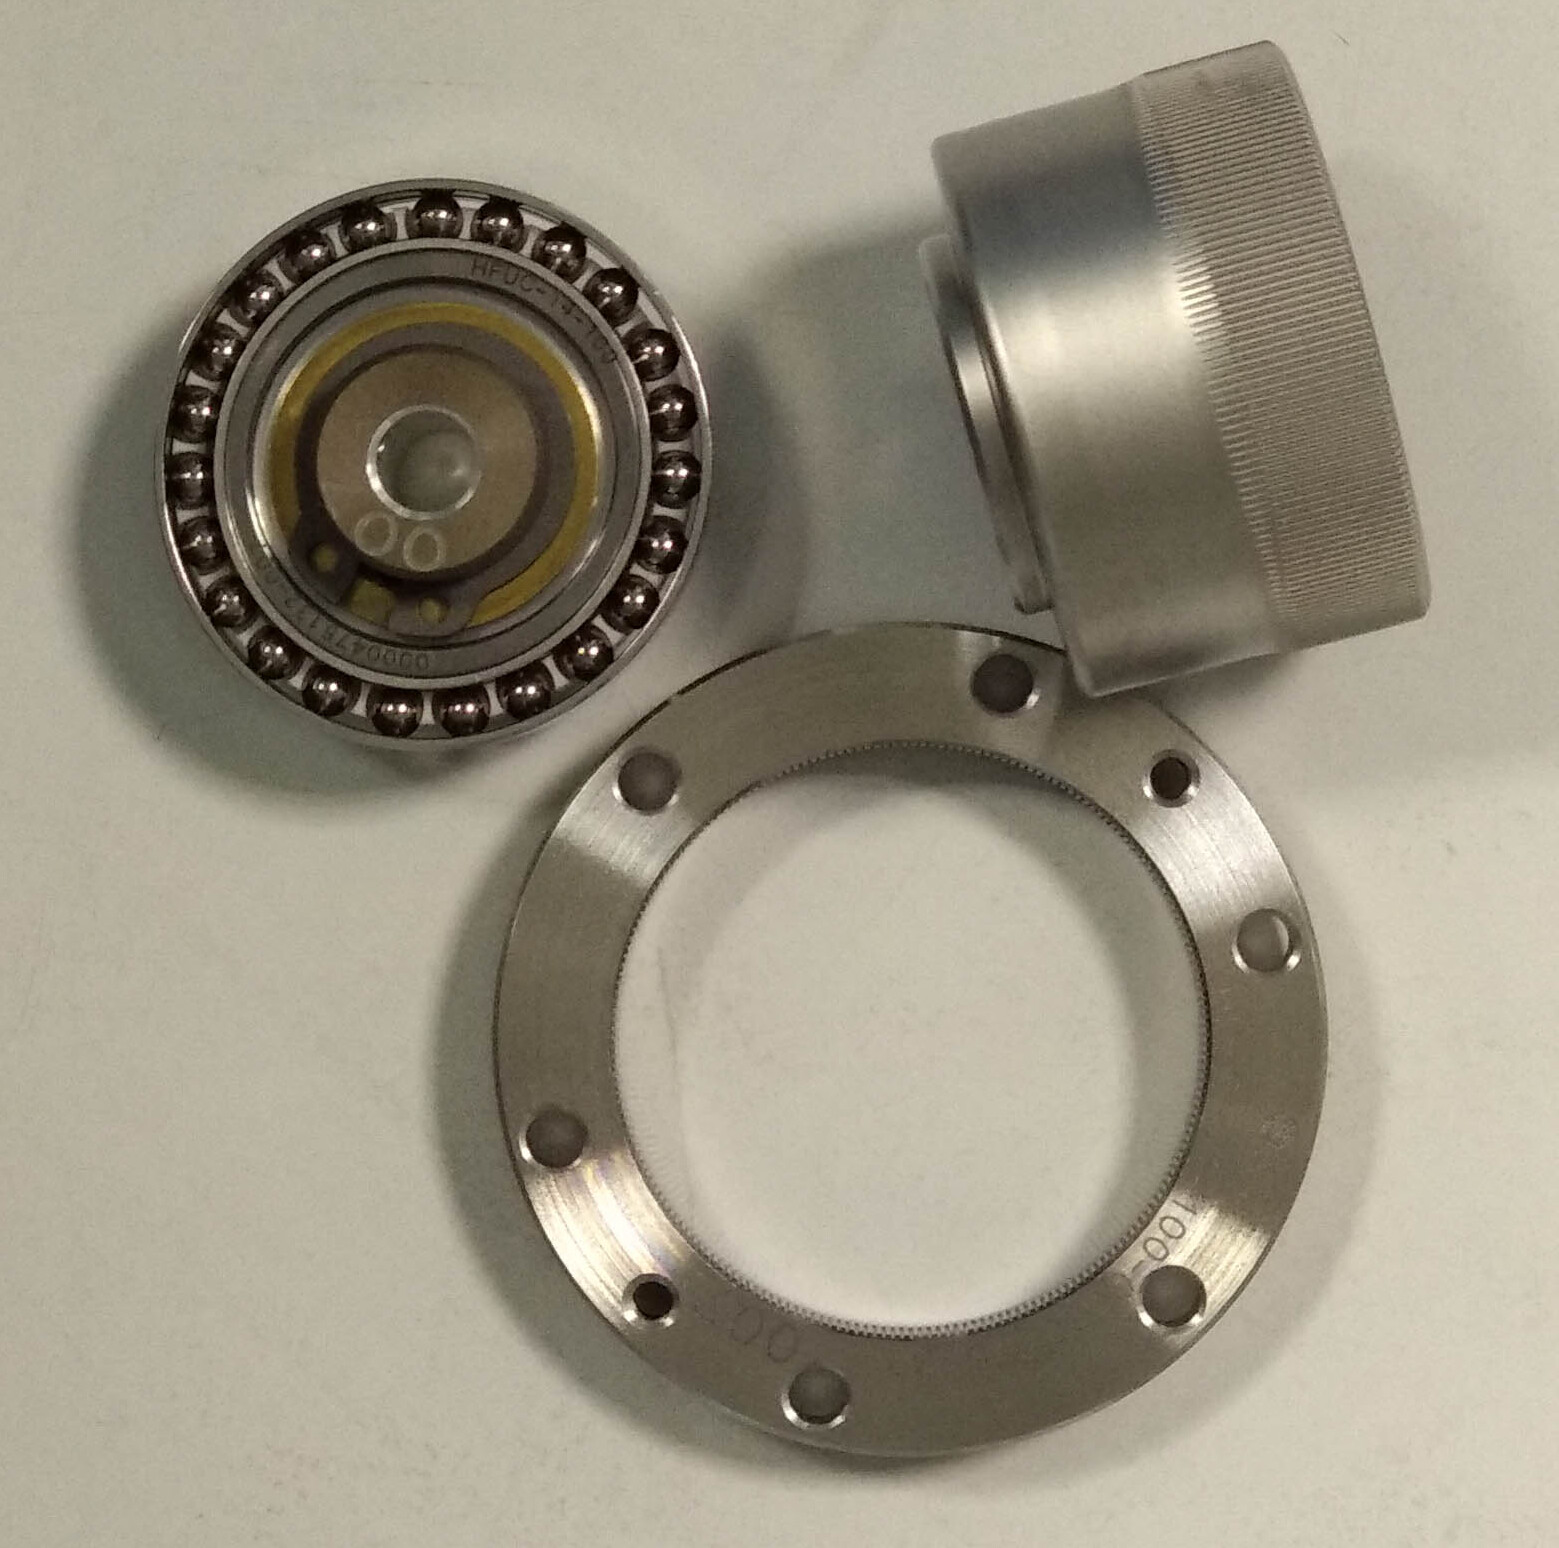
\includegraphics[width=0.45\linewidth,height=\textheight,keepaspectratio]{chapters/02-body/figures/fig02_real_strain_wave_gear.jpg}

}

\caption{\label{fig-02-real-strain-wave-gear}\textbf{Strain Wave
(Harmonic Drive) Gear Component Set and Mechanical Coupling.} Authentic
component set of a robotic strain wave gear transmission (Harmonic Drive
AG). The assembly comprises the elliptical wave generator with thin-race
ball bearings (top left), the thin-walled flexible cup flexspline with
external gear teeth (top right), and the rigid circular spline with
internal gear teeth (bottom). Elastic deformation of the flexspline
allows high single-stage gear reduction (typically \(50:1\) to
\(160:1\)) with near-zero initial backlash, but introduces significant
torsional compliance, mechanical hysteresis, and structural fatigue
limits under dynamic shock loads.}

\end{figure}%

\begin{figure}[t]

\centering{

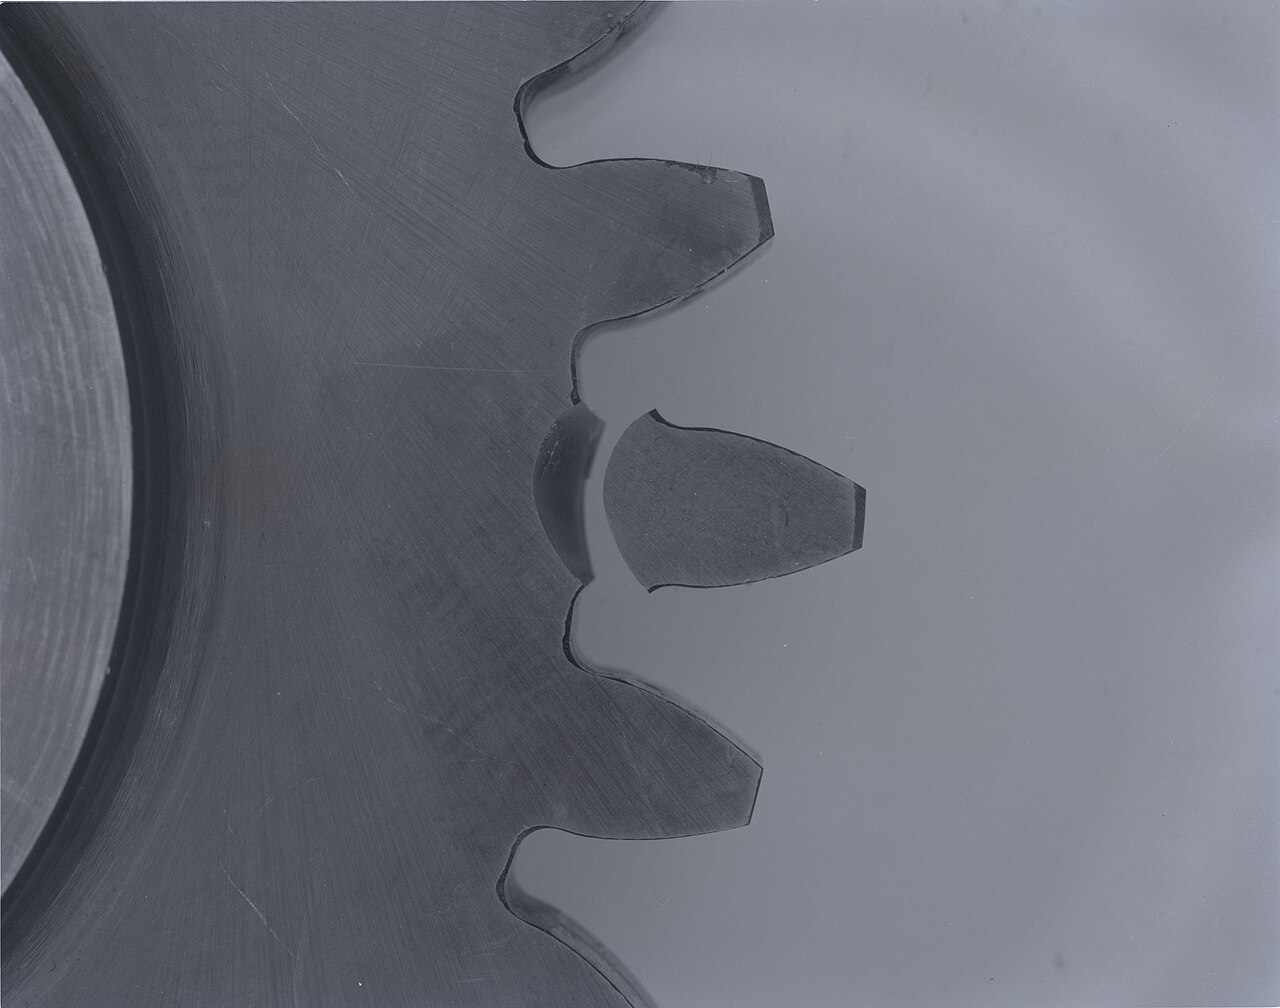
\includegraphics[width=0.55\linewidth,height=\textheight,keepaspectratio]{chapters/02-body/figures/fig02_real_broken_gear_tooth.jpg}

}

\caption{\label{fig-02-real-broken-gear-tooth}\textbf{Catastrophic Gear
Tooth Root Fatigue Fracture from Dynamic Shock Loads.} Macro-fracture of
a high-torque transmission gear tooth undergoing cyclic stress testing
at NASA Glenn Research Center. When a high-ratio geared transmission
(\(N \ge 50\)) experiences discontinuous policy torque steps or sudden
external impact, reflected rotor inertia
(\(J_{\text{ref}} = N^2 J_{\text{rotor}}\)) prevents the rotor from
backdriving. The kinetic energy concentrates entirely as mechanical
shear stress at the tooth root fillet, causing catastrophic fatigue
fracture rather than reporting a software error.}

\end{figure}%

Selecting an appropriate mechanical transmission architecture
establishes the fundamental systems trade-offs between continuous torque
density and backdrivability, as summarized in
table~\ref{tbl-02-mechanical-drives}.

\begin{longtable}[]{@{}
  >{\raggedright\arraybackslash}p{(\linewidth - 6\tabcolsep) * \real{0.2500}}
  >{\raggedright\arraybackslash}p{(\linewidth - 6\tabcolsep) * \real{0.2500}}
  >{\raggedright\arraybackslash}p{(\linewidth - 6\tabcolsep) * \real{0.2500}}
  >{\raggedright\arraybackslash}p{(\linewidth - 6\tabcolsep) * \real{0.2500}}@{}}
\caption{\textbf{Comparative Systems Matrix of Actuator Transmission
Mechanisms.} Quantitative trade-offs across robotic drive mechanisms,
mapping reduction ratio (\(N\)), reflected rotor inertia scaling
(\(N^2\)), and operational implications for learned control
policies.}\label{tbl-02-mechanical-drives}\tabularnewline
\toprule\noalign{}
\begin{minipage}[b]{\linewidth}\raggedright
Transmission Archetype
\end{minipage} & \begin{minipage}[b]{\linewidth}\raggedright
Gear Ratio (\(N\))
\end{minipage} & \begin{minipage}[b]{\linewidth}\raggedright
Reflected Inertia (\(N^2\))
\end{minipage} & \begin{minipage}[b]{\linewidth}\raggedright
Implication for Physical AI Policies
\end{minipage} \\
\midrule\noalign{}
\endfirsthead
\toprule\noalign{}
\begin{minipage}[b]{\linewidth}\raggedright
Transmission Archetype
\end{minipage} & \begin{minipage}[b]{\linewidth}\raggedright
Gear Ratio (\(N\))
\end{minipage} & \begin{minipage}[b]{\linewidth}\raggedright
Reflected Inertia (\(N^2\))
\end{minipage} & \begin{minipage}[b]{\linewidth}\raggedright
Implication for Physical AI Policies
\end{minipage} \\
\midrule\noalign{}
\endhead
\bottomrule\noalign{}
\endlastfoot
\textbf{Direct Drive (No Gearing)} & \(1:1\) (\(N = 1\)) & \(N^2 = 1\)
(Minimal) & Transparently backdrivable; absorbs impact shocks; limited
continuous torque density
(\(\sim 2\text{--}5\text{ N}\cdot\text{m/kg}\)). \\
\textbf{Quasi-Direct Drive (QDD)} & \(3:1\text{--}10:1\) (\(N \le 10\))
& \(N^2 \le 100\) (Low) & High backdrivability; enables proprioceptive
torque sensing via motor current; high impact tolerance for dynamic
quadrupeds and arms. \\
\textbf{High-Ratio Geared (Planetary / Harmonic)} &
\(30:1\text{--}160:1\) (\(N \ge 30\)) & \(N^2 \ge 900\text{--}25{,}000\)
(Extreme) & High torque density for heavy payloads; non-backdrivable;
high-frequency policy chatter causes inverter current saturation and
tooth shear. \\
\textbf{Open-Loop Stepper Motor} & \(1:1\) (High pole count) &
\(N^2 = 1\) & High static holding torque at zero speed; silent state
loss (``lost steps'') when commanded acceleration exceeds magnetic
pull-out torque. \\
\end{longtable}

\protect\phantomsection\label{callout-archetypeux2a-2.9}
\begin{fbxSimple}{callout-archetype}{Archetype Focus:}{Class 2 Contact-Dominated Manipulation Systems}
\phantomsection\label{callout-archetype*-2.9}

In Class 2 machines (articulated robot arms, multi-fingered hands, and
contact-rich assembly workcells), the primary physical failure mode is
\textbf{destructive contact force spikes and drive-train tooth shear}.
When a robot arm makes unexpected contact with a rigid environment of
stiffness \(k\), contact force spikes at \(F = k \Delta x\). If the
joint employs a high gear reduction (\(N \ge 50\)), the reflected rotor
inertia
\(J_{\text{ref}} = N^2 J_{\text{rotor}} \ge 2500 J_{\text{rotor}}\)
prevents external impact forces from backdriving the motor. The kinetic
impact cannot be converted into electrical regeneration; instead, the
shock load concentrates entirely as mechanical shear stress across the
gear teeth. For contact-dominated manipulation, neural policies must
either be paired with backdrivable Quasi-Direct Drive (QDD) actuators
(which enable proprioceptive current sensing without external load
cells) or filtered through real-time torque limiters and impedance
controllers.

\end{fbxSimple}

For the physical AI systems engineer, these electromechanical realities
dictate two foundational design rules. First, raw neural network outputs
must never be mapped directly to joint motor inverters without smooth
continuous motion profiling; the real-time microcontroller must
interpolate discrete action chunks through \(C^2\)-continuous splines
(such as quintic polynomials or S-curve limiters) to bound commanded
jerk and prevent current saturation against reflected rotor inertia.
Second, closed-loop safety verification cannot rely solely on motor-side
encoders; the engineer must place absolute encoders and torque sensors
directly on the output load side of the transmission, ensuring that
silent mechanical failures---such as flexspline tooth fracture, shaft
shear, or transmission backlash---are immediately detected and
intercepted before damaging the workcell.

Operating continuously near current and torque limits extracts an
irreversible thermodynamic cost. Every ampere driven through the stator
winding to overcome rotor inertia or sustain peak output torque
dissipates resistive heat (\(I^2 R\)) directly into the copper coils.
While magnetic flux builds within milliseconds, the heat it generates
accumulates in the physical thermal mass of the actuator over seconds
and minutes, creating a thermal clock that bounds how long peak torque
can be delivered before insulation breaks down.

\section{Thermal Limits and Duty Cycle}\label{sec-body-2-5}

Holding a \(25\text{ kg}\) cast iron workpiece motionless in mid-air
places a deceptive demand on an articulated robot. In simulation, an
artificial intelligence agent can sustain static holding torque
indefinitely without penalty. On physical hardware, holding a static
load against gravity requires continuous phase current through the
stator coils. \textbf{Heat arrives in seconds and leaves in minutes,
making duty cycle a primary design variable rather than a thermal
footnote.}

While mechanical momentum can be redirected and magnetic flux decays
within milliseconds of opening a switch, thermal energy has no fast
physical exit. Thermal capacity is the physical integral of power loss
over time. What that capacity protects is a specific, inflexible
material threshold, namely the dielectric rating of the stator winding
insulation and the Curie temperature of permanent rotor magnets
(figure~\ref{fig-02-real-burnt-motor-stator}). Modern motor windings use
polymer enamel coatings classified under standards such as IEC 60085,
where Class F insulation withstands a maximum continuous hotspot
temperature of \(155^\circ\text{C}\) and Class H withstands
\(180^\circ\text{C}\). Exceeding this rating softens the polymer matrix,
causing inter-turn shorts that destroy the phase winding.
Neodymium-iron-boron (\(\text{NdFeB}\)) rotor magnets face a companion
limit, where temperatures between \(80^\circ\text{C}\) and
\(150^\circ\text{C}\) cause irreversible demagnetization under strong
stator demagnetizing fields.

\begin{figure}[t]

\centering{

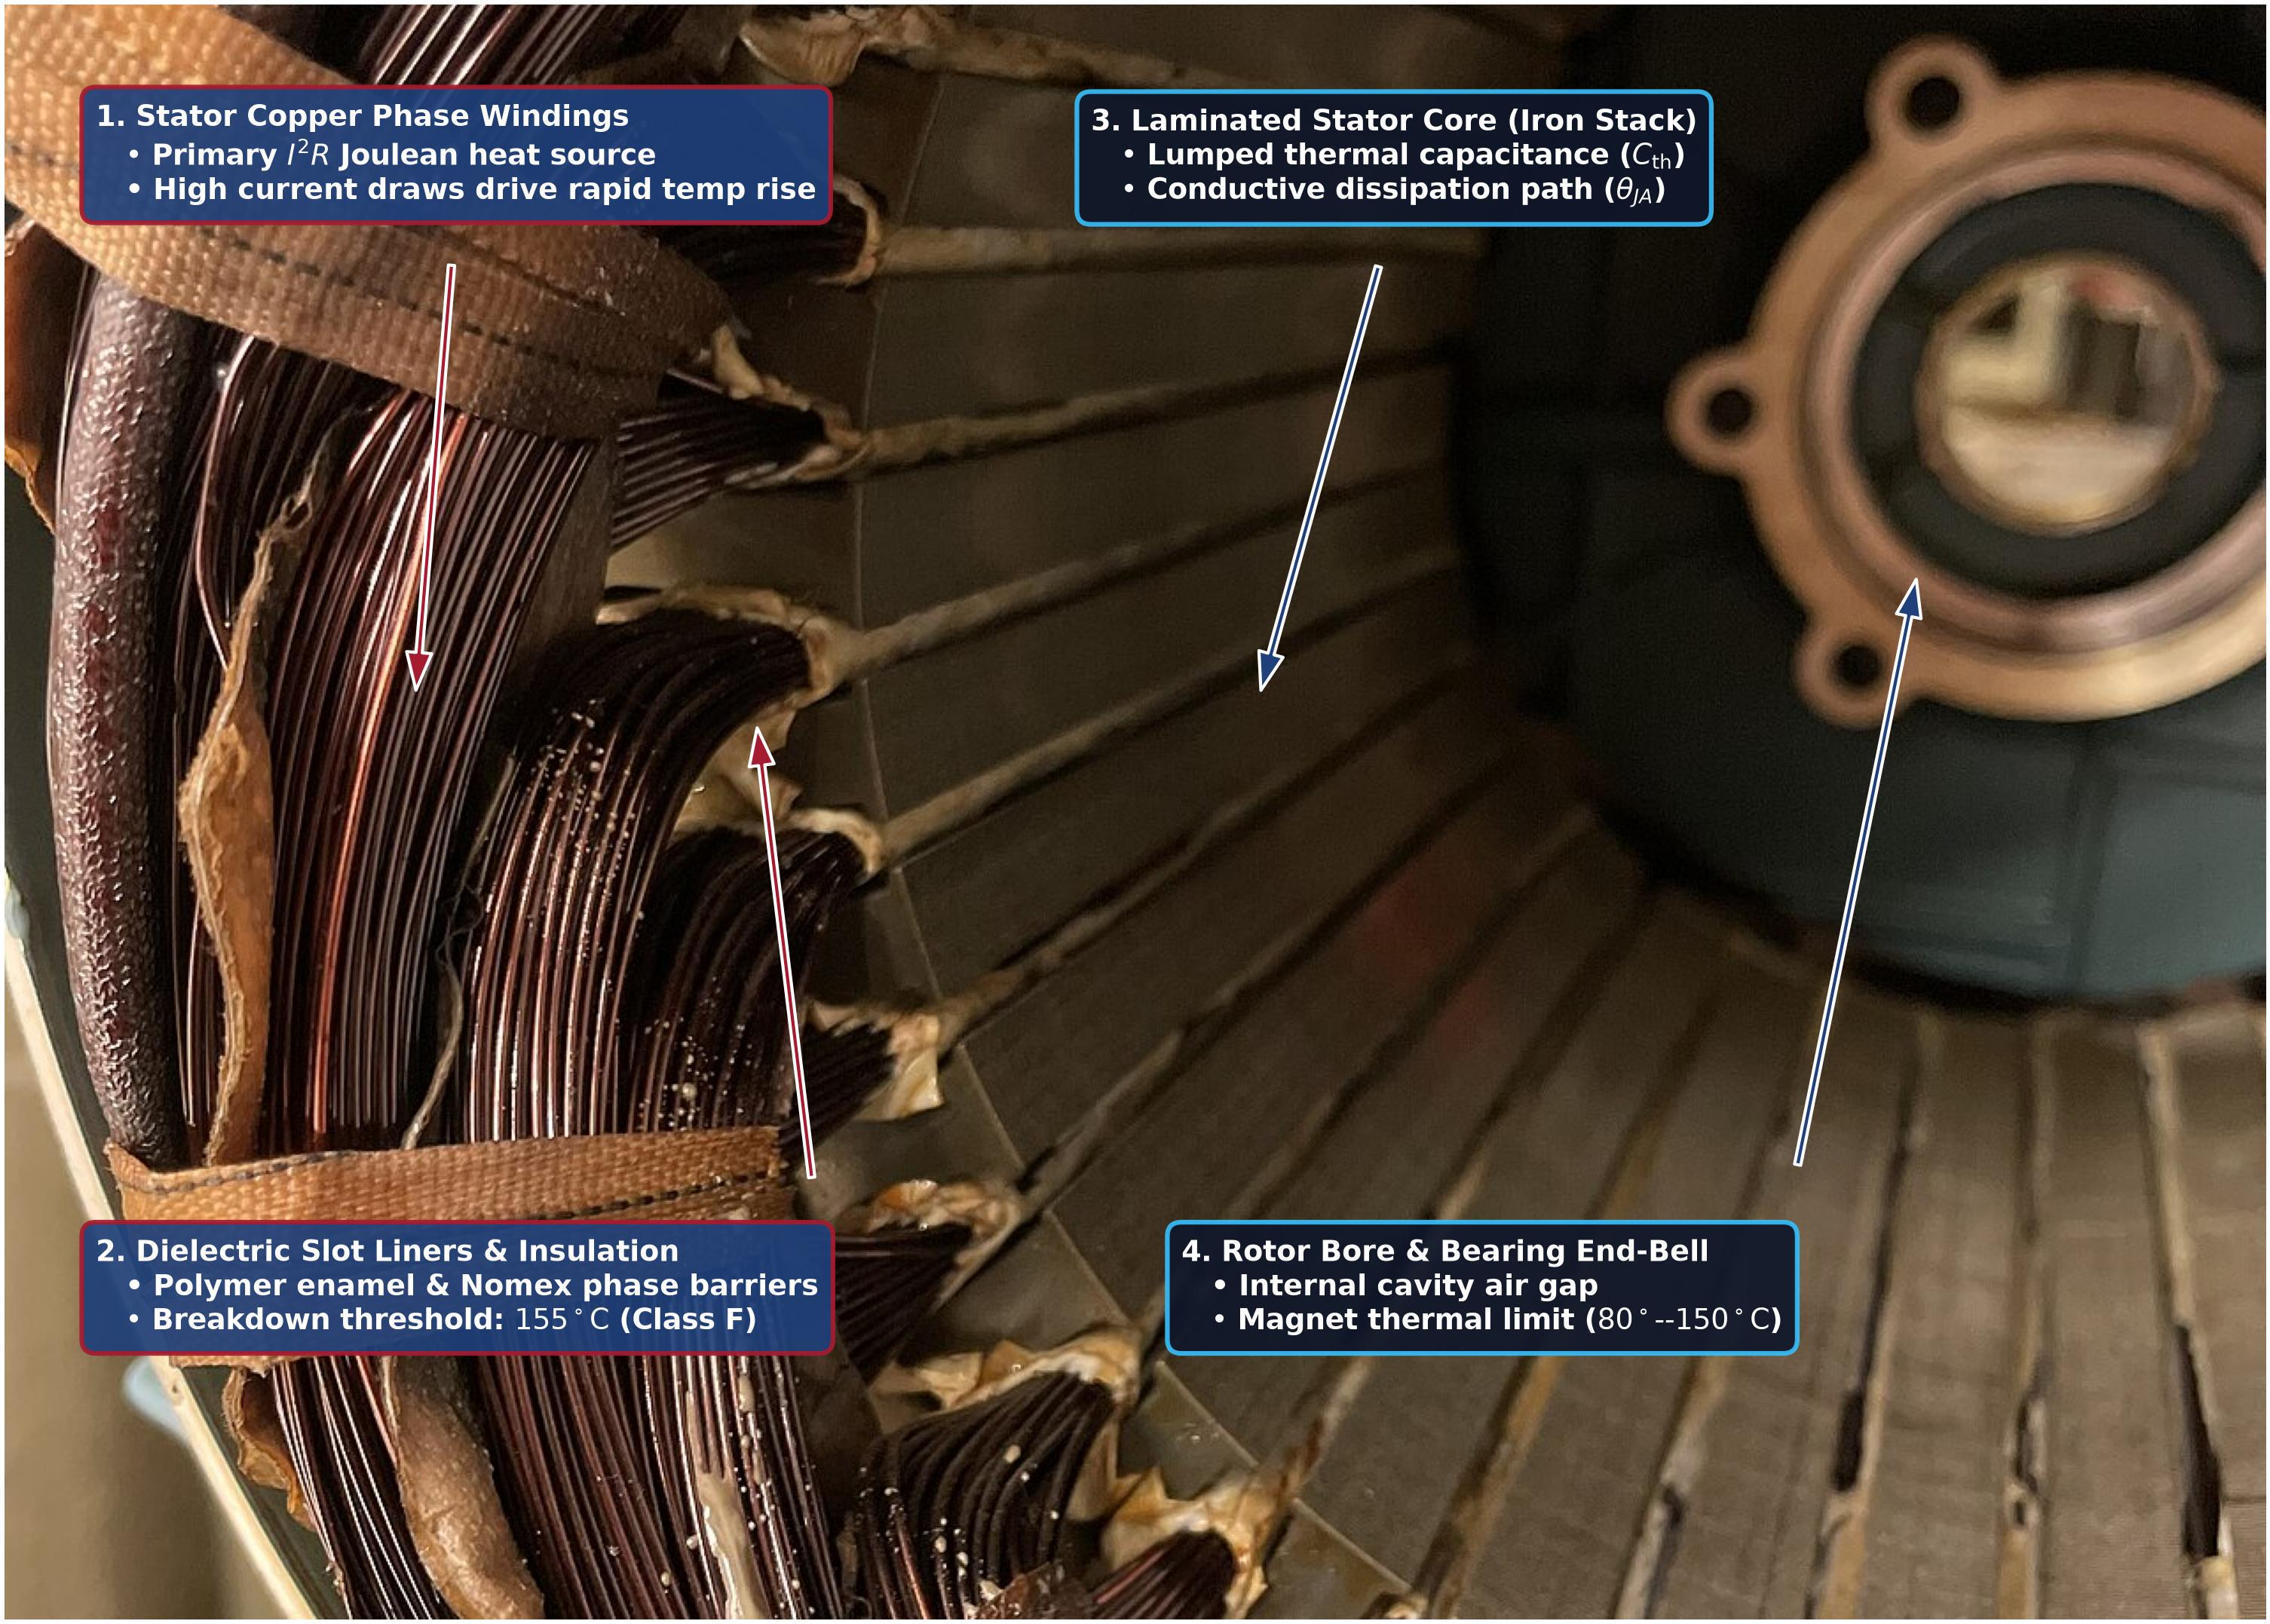
\includegraphics[width=0.65\linewidth,height=\textheight,keepaspectratio]{chapters/02-body/figures/fig02_real_burnt_motor_stator.jpg}

}

\caption{\label{fig-02-real-burnt-motor-stator}\textbf{Irreversible
Stator Winding Insulation Breakdown from Unmanaged Overheating.}
Internal view of an electric motor stator suffering severe thermal
degradation. Continuous high-current operation (\(I^2 R\)) without
sufficient thermal recovery intervals (\(t_{\text{off}}\)) heats stator
copper beyond the dielectric temperature rating of its Class F/H polymer
enamel coating (\(155^\circ\text{C}\)--\(180^\circ\text{C}\)). The
charred slot liners and darkened copper coils indicate inter-turn
insulation failure, leading to catastrophic phase-to-phase short
circuits. (Source: Industrial Electromechanical Diagnostics Archive, CC
BY 4.0).}

\end{figure}%

The rate of heat generation follows directly from the current commanded
through the motor phases. For an instantaneous phase current \(I(t)\)
and winding resistance \(R(T)\), resistive Joulean dissipation dumps
thermal power into the stator copper according to the relation
\(P_{\text{loss}}(t) = I^2(t) R(T)\).\sidenote{\footnotesize Stator copper resistance
  increases by \(+47.1\%\) between \(20^\circ\text{C}\) and
  \(140^\circ\text{C}\) (\(R(T) = R_0[1 + \alpha_{\text{Cu}}(T-T_0)]\)),
  inflating \(I^2 R\) heat generation during heavy duty cycles. Winding
  temperatures are monitored via RTDs or NTC thermistors linearized via
  Steinhart-Hart equations on microcontroller ADCs.} This thermal power
divides between heating the physical thermal capacitance of the winding
\(C_{\text{th}}\) and conducting heat across the stator-to-ambient
thermal resistance \(\theta_{JA}\) (also denoted \(R_{\text{th}}\)) to
the motor casing and surrounding air. The governing first-order
thermodynamic differential equation is
\[C_{\text{th}} \frac{dT(t)}{dt} = P_{\text{loss}}(t) - \frac{T(t) - T_{\text{amb}}}{\theta_{JA}} = I^2(t) R(T) - \frac{T(t) - T_{\text{amb}}}{\theta_{JA}}\]
Defining the thermal time constant \(\tau = \theta_{JA} C_{\text{th}}\),
the temperature trajectory for a constant power loss \(P_{\text{loss}}\)
starting from an initial temperature \(T(0)\) integrates to
\[T(t) = T_{\text{amb}} + (T(0) - T_{\text{amb}}) e^{-t/\tau} + P_{\text{loss}} \theta_{JA} \left(1 - e^{-t/\tau}\right)\]
In the steady-state limit as \(t \to \infty\), the equilibrium
temperature rise above ambient is
\[\Delta T_{\text{ss}} = T_{\text{ss}} - T_{\text{amb}} = P_{\text{loss}} \theta_{JA} = I^2 R(T_{\text{ss}}) \theta_{JA}\]

This formulation exposes why stator thermal limits create a hard,
non-negotiable physical boundary for machine learning policies. Neural
policies trained in simulation environments (such as Isaac Gym, MuJoCo,
or PyBullet) optimize reward functions where torque is treated as an
instantaneous, massless mathematical variable. In simulation, a policy
can hold a heavy payload indefinitely, stiffen joint impedance through
continuous high-torque antagonist co-contraction, or chatter rapidly
across contact boundaries without incurring any physical consequence. On
real physical hardware, sustained current \(I\) pumps thermal energy
into stator copper at an adiabatic initial rate
\(dT/dt \approx I^2 R / C_{\text{th}}\).

This thermodynamic cost is compounded by the positive temperature
coefficient of copper
(\(\alpha_{\text{Cu}} \approx 0.00393\text{ K}^{-1}\)). As the stator
temperature climbs from \(20^\circ\text{C}\) toward its
\(140^\circ\text{C}\) engineering ceiling, phase resistance increases by
over \(47\%\) according to the linear relation
\(R(T) = R_0 [1 + \alpha_{\text{Cu}}(T - T_0)]\). To sustain identical
commanded torque (\(\tau = K_t I\)), the inverter must deliver higher
phase voltage, dissipating \(47\%\) more resistive power (\(I^2 R(T)\))
at the exact moment thermal cooling is least effective. If an
unconstrained neural policy commands continuous peak torque, this
positive thermal feedback accelerates the winding toward dielectric
breakdown in tens of seconds.

\protect\phantomsection\label{callout-archetypeux2a-2.10}
\begin{fbxSimple}{callout-archetype}{Archetype Focus:}{Class 3 Flow-Dominated Process and Thermal Plants}
\phantomsection\label{callout-archetype*-2.10}

In Class 3 systems (grid-scale battery energy storage, liquid cooling
distribution units, and continuous thermal regulation plants), the
primary physical failure mode is \textbf{irreversible thermal
accumulation and runaway}. Unlike mechanical momentum which can be
redirected or arrested by mechanical brakes, thermal energy has no fast
physical exit: heat arrives in seconds
(\(dT/dt \approx P_{\text{loss}} / C_{\text{th}}\)) but leaves across
minutes through thermal resistance (\(\theta_{JA}\)). For physical AI
controllers regulating fluid and power plants, learned policies cannot
optimize short-term throughput at the expense of steady-state heat
balance without inducing unrecoverable thermal trips.

\end{fbxSimple}

Datasheet thermal specifications provide an optimistic baseline because
manufacturers measure them under idealized laboratory conditions,
typically mounting an unconstrained motor to a large aluminum heat sink
in free air at \(20^\circ\text{C}\) or \(25^\circ\text{C}\). On an
operational machine, the actuator operates inside a sealed chassis
alongside power electronics, battery packs, and adjacent joint motors.
Enclosing the motor eliminates ambient convective airflow, increasing
the effective thermal resistance \(\theta_{JA}\). Furthermore,
neighboring computation and power conversion stages dump heat into the
shared structural chassis, raising the local internal ambient
temperature \(T_{\text{amb}}\) well above external room temperature. A
joint actuator operating near a graphics processor or battery pack can
experience a local ambient of \(45^\circ\text{C}\) to
\(55^\circ\text{C}\) before its own coils carry current. Accurately
budgeting thermal margins requires measuring the installed heating and
cooling time constants with the enclosure fully sealed and all adjacent
electrical loads operating at their \(P_{99}\) power draw.

Because thermal capacity integrates power over time, a peak torque or
peak current rating on a motor datasheet is physically meaningless
without four accompanying parameters, specifically the initial winding
temperature \(T(0)\), the maximum allowable duration \(t_{\text{on}}\),
the operating ambient temperature \(T_{\text{amb}}\), and the required
recovery duration \(t_{\text{off}}\). An actuator capable of producing
three times its continuous rated torque can sustain that load only while
the integral of \(I^2 R\) remains within the thermal margin below the
insulation limit. If the winding begins at room temperature, that burst
can last tens of seconds. If the winding is already soaked at its
continuous operating temperature from sustained motion, the identical
current pulse reaches the insulation threshold in a fraction of that
time.

Consider the thermal budgeting for the shoulder joint of our
heavy-payload arm, with winding resistance \(R = 1.2\ \Omega\), lumped
thermal capacitance \(C_{\text{th}} = 120\text{ J/K}\), and an installed
thermal resistance \(\theta_{JA} = 2.5\text{ K/W}\), yielding a thermal
time constant \(\tau = 300\text{ s}\) (\(5.0\text{ min}\)). The motor
uses Class F insulation rated to \(155^\circ\text{C}\) and operates in
an enclosed internal ambient \(T_{\text{amb}} = 40^\circ\text{C}\). At
its continuous rated current \(I_{\text{cont}} = 5.0\text{ A}\), the
steady-state resistive loss is
\(P_{\text{cont}} = (5.0\text{ A})^2 \times 1.2\ \Omega = 30.0\text{ W}\),
producing an equilibrium temperature rise of
\(\Delta T_{\text{cont}} = 30.0\text{ W} \times 2.5\text{ K/W} = 75.0\text{ K}\)
and an equilibrium operating temperature of \(115^\circ\text{C}\),
safely below the material rating. When a learned policy commands peak
torque requiring \(I_{\text{peak}} = 15.0\text{ A}\) (\(3.0\times\)
continuous rating) to accelerate the workpiece, resistive power
dissipation jumps by a factor of nine to
\(P_{\text{peak}} = (15.0\text{ A})^2 \times 1.2\ \Omega = 270.0\text{ W}\).
If sustained indefinitely, this loss would drive asymptotic temperature
to
\(T_{\text{amb}} + P_{\text{peak}} \theta_{JA} = 40^\circ\text{C} + 270.0\text{ W} \times 2.5\text{ K/W} = 715^\circ\text{C}\),
destroying the winding. Starting cold at \(T(0) = 40^\circ\text{C}\),
the time \(t\) to reach the \(155^\circ\text{C}\) insulation limit
satisfies \(155 = 40 + 675 (1 - e^{-t / 300})\), which evaluates to
\(t = -300 \ln(1 - 115 / 675) \approx 56.0\text{ s}\). If the motor was
already operating at its continuous thermal equilibrium of
\(115^\circ\text{C}\), the same \(15.0\text{ A}\) command drives the
winding to \(155^\circ\text{C}\) according to
\(155 = 715 - (715 - 115) e^{-t / 300}\), reaching the failure boundary
in just \(t = -300 \ln(560 / 600) \approx 20.7\text{ s}\).

To prevent winding degradation under repeated motion cycles with period
\(t_{\text{cycle}} = t_{\text{on}} + t_{\text{off}}\), the machine must
operate within a safe cyclic steady-state temperature profile. Enforcing
an engineering ceiling \(T_{\text{max}} = 140^\circ\text{C}\) to
preserve a \(15^\circ\text{C}\) safety buffer below the insulation limit
restricts the allowable temperature rise above ambient to
\(\Delta T_{\text{allow}} = 140^\circ\text{C} - 40^\circ\text{C} = 100\text{ K}\).
The maximum permissible average power dissipation over the cycle is
\(\bar{P}_{\text{max}} = \Delta T_{\text{allow}} / \theta_{JA} = 100\text{ K} / 2.5\text{ K/W} = 40.0\text{ W}\).
For a profile that alternates between peak torque dissipation
\(P_{\text{peak}} = 270.0\text{ W}\) during \(t_{\text{on}}\) and zero
current during \(t_{\text{off}}\), the time-averaged power is
\(\bar{P} = D P_{\text{peak}}\), where
\(D = t_{\text{on}} / t_{\text{cycle}}\) is the duty cycle. Bounding
\(\bar{P} \le 40.0\text{ W}\) constrains the allowable duty cycle to:
\[D \le \frac{T_{\text{max}} - T_{\text{amb}}}{P_{\text{peak}} \theta_{JA}} = \frac{\Delta T_{\text{allow}}}{I_{\text{peak}}^2 R(T_{\text{max}}) \theta_{JA}} = \frac{40.0\text{ W}}{270.0\text{ W}} \approx 0.148 \quad (14.8\%)\]

Just as a computer architect cannot run a processor at peak boost clock
indefinitely without violating its Thermal Design Power (TDP), a
physical AI architect cannot command peak actuator torque without
depleting the thermal capacity of the motor windings. Because Joulean
heat arrives in seconds (\(P = I^2 R\)) while dissipation through
conduction and natural convection takes minutes
(\(\tau = \theta_{JA} C_{\text{th}} \approx 300\text{ s}\)), peak bursts
require a mandatory thermal recovery interval:
\[t_{\text{off}} = t_{\text{on}} \left( \frac{1 - D}{D} \right)\] If a
learned policy commands a \(3.0\text{ s}\) peak torque burst to brace
against an unpredicted load disturbance, the nervous system must enforce
a recovery interval of at least \(t_{\text{off}} \approx 17.3\text{ s}\)
before peak torque can be safely granted again.

\protect\phantomsection\label{callout-mathux2a-2.11}
\begin{fbxSimple}{callout-math}{Napkin Math:}{Adiabatic Stator Thermal Spike under Peak Torque Stall}
\phantomsection\label{callout-math*-2.11}

\emph{Problem:} A robotic manipulator shoulder actuator features stator
copper windings with total mass \(m_{\text{Cu}} = 0.35\text{ kg}\)
(copper specific heat capacity
\(c_{\text{Cu}} = 385\text{ J}/(\text{kg}\cdot\text{K})\), yielding
lumped thermal capacitance
\(C_{\text{th}} = m_{\text{Cu}} c_{\text{Cu}} = 134.75\text{ J/K}\)).
Nominal room-temperature phase resistance is
\(R(20^\circ\text{C}) = 0.60\ \Omega\), and installed thermal resistance
to ambient (\(T_{\text{amb}} = 40^\circ\text{C}\)) is
\(\theta_{JA} = 2.2\text{ K/W}\). The motor operates with Class F
insulation (\(T_{\text{ins}} = 155^\circ\text{C}\), enforced limit
\(T_{\max} = 140^\circ\text{C}\)). When a neural policy commands peak
holding torque drawing \(I_{\text{peak}} = 22.0\text{ A}\) from a
pre-warmed operating temperature \(T(0) = 65^\circ\text{C}\), what is
the initial heating rate, and how long until the winding reaches thermal
breakdown?

\textbf{1. Initial Joulean Dissipation (\(P_{\text{loss}}\)) with Copper
Temperature Effect:} At \(T(0) = 65^\circ\text{C}\), winding resistance
has increased under the copper temperature coefficient
(\(\alpha_{\text{Cu}} = 0.00393\text{ K}^{-1}\)):
\[R(65^\circ\text{C}) = R_0 [1 + \alpha_{\text{Cu}}(65 - 20)] = 0.60 \times [1 + 0.00393 \times 45] = 0.60 \times 1.177 = 0.706\ \Omega\]
Instantaneous Joulean thermal dissipation is:
\[P_{\text{loss}} = I_{\text{peak}}^2 R(65^\circ\text{C}) = (22.0\text{ A})^2 \times 0.706\ \Omega = 484 \times 0.706 = 341.7\text{ W}\]

\textbf{2. Initial Adiabatic Heating Rate (\(dT/dt\)):} Before thermal
conduction to ambient takes effect
(\(t \ll \tau = \theta_{JA} C_{\text{th}} \approx 296\text{ s}\)), heat
accumulation is near-adiabatic:
\[\left.\frac{dT}{dt}\right|_{t=0} \approx \frac{P_{\text{loss}}}{C_{\text{th}}} = \frac{341.7\text{ W}}{134.75\text{ J/K}} \approx 2.54^\circ\text{C/s}\]

\textbf{3. Time to Insulation Breakdown Threshold
(\(T_{\max} = 140^\circ\text{C}\)):} Asymptotic steady-state temperature
if sustained would reach
\(T_{\text{ss}} = T_{\text{amb}} + P_{\text{loss}} \theta_{JA} = 40 + 341.7 \times 2.2 = 791.7^\circ\text{C}\).
Solving the transient thermal trajectory
\(140 = 791.7 - (791.7 - 65) e^{-t / 296}\):
\[e^{-t / 296} = \frac{791.7 - 140}{791.7 - 65} = \frac{651.7}{726.7} \approx 0.8968\]
\[t = -296 \times \ln(0.8968) \approx -296 \times (-0.1089) \approx 32.2\text{ seconds}\]
In just \(32.2\text{ seconds}\) of peak stall, the motor destroys its
insulation unless derated.

\end{fbxSimple}

Because thermal accumulation is an integral state with time constants
spanning hundreds of seconds, an agent trained in simulation has no
intrinsic incentive to preserve winding health. The systems engineer
must implement a real-time discrete \(I^2 t\) thermal observer directly
on the deterministic microcontroller, sampling phase currents across
low-side shunt resistors (\(R_{\text{shunt}}\)) at \(1000\text{ Hz}\) to
track estimated coil hotspot temperatures:
\[T_{k+1} = T_k + \frac{\Delta t}{C_{\text{th}}} \left[ I_{\text{meas}, k}^2 R(T_k) - \frac{T_k - T_{\text{amb}}}{\theta_{JA}}\right]\]
where \(R(T_k) = R_0 [1 + \alpha_{\text{Cu}}(T_k - T_0)]\). If estimated
temperature \(T_{k+1}\) crosses the derating ceiling
\(T_{\max} = 140^\circ\text{C}\), the safety enforcer scales candidate
policy currents by a dynamic derating factor
\(\gamma = \max\left(0.0, \frac{T_{\text{trip}} - T_{k+1}}{T_{\text{trip}} - T_{\max}}\right)\),
clamping commands to
\(I_{\text{cmd}} = \min(I_{\text{cand}}, \gamma I_{\text{cont}})\). If
\(T_{k+1} \ge T_{\text{trip}} = 155^\circ\text{C}\), the microcontroller
trips an emergency thermal shutdown (\(I_{\text{cmd}} = 0\)), vetoing
the learned policy before dielectric breakdown occurs.

Delivering the large current pulses that generate these thermal loads
simultaneously stresses the upstream electrical supply, transferring the
physical burden from thermal dissipation in copper to transient current
delivery across the power bus.

\section{Power and Electrical Faults}\label{sec-body-2-6}

When an agile quadruped or mobile manipulator executes an explosive
evasive maneuver---a rapid multi-joint lunge to avoid an oncoming
collision---every drive motor, joint inverter, and neural accelerator
demands maximum current simultaneously from a single direct-current
distribution bus. In simulation, current flows frictionlessly from an
idealized numerical source. On physical hardware, a machine that browns
out mid-motion fails physically, and the electrical supply is a shared
resource governed by finite capacity and transient limits. \textbf{A
machine that browns out mid-motion fails physically, and the electrical
supply is a shared resource like any other.}

Rail sag, regenerative overvoltage, and thermal accumulation are not
separate electrical phenomena, but different temporal manifestations of
the same bounded energy network. While winding heating reflects energy
accumulated over seconds as thermal dissipation in copper, voltage
fluctuations occur across microseconds and milliseconds whenever current
demand exceeds instantaneous source capacity. Onboard compute units,
neural network accelerators, sensing payloads, and motor inverters all
draw from a common direct-current distribution bus. When a learned
policy commands aggressive, coordinated accelerations across multiple
joints, the resulting sum of simultaneous current draws alters the
operating voltage delivered to every node on the machine.

The total current demand on the power rail is the sum of instantaneous
consumer currents,
\(I_{\text{bus}}(t) = I_{\text{compute}}(t) + I_{\text{sensors}}(t) + \sum_{k=1}^N I_{\text{actuator},k}(t)\).
The physical supply cannot deliver infinite current instantaneously.
Every electrical distribution bus exhibits a non-zero source impedance
\(R_{\text{bus}}\),\sidenote{\footnotesize Total bus impedance \(R_{\text{bus}}\)
  combines battery internal resistance
  (\(12\text{--}20\text{ m}\Omega/\text{cell}\)), wiring harness
  resistance, and power connectors. When high-acceleration current
  spikes pull bus potential below microcontroller Brownout Reset (BOR)
  thresholds (e.g., canonical microcontroller BOR registers), hardware
  asserts an asynchronous reset on \texttt{NRST}.} combining the
internal resistance of the battery or power supply and the resistance of
wiring harnesses, connectors, and protection switches. Bulk decoupling
capacitors with total capacitance \(C_{\text{bus}}\) provide local
charge storage to smooth fast load transients. When the policy demands a
rapid step change in total current \(\Delta I_{\text{step}}\) with
risetime \(\Delta t\), the current ramps at a rate
\(dI/dt \approx \Delta I_{\text{step}} / \Delta t\). Before the primary
power supply or battery chemistry can adjust its chemical reaction rate
or control loop over its response window \(\tau_{\text{reg}}\), the bus
voltage drops by an amount determined by the resistive drop and the
capacitive charge depletion. The total transient droop is given by:
\[\Delta V_{\text{droop}} = \Delta I_{\text{step}} R_{\text{bus}} + \frac{1}{C_{\text{bus}}} \int_0^{\Delta t} I_{\text{step}}(t) \, dt \approx \Delta I_{\text{step}} R_{\text{bus}} + \frac{\Delta I_{\text{step}} \Delta t}{2 C_{\text{bus}}}.\]

The opposite boundary occurs during deceleration, where kinetic energy
stored in moving mass returns to the electrical bus. \textbf{Braking
does not discard energy, but converts mechanical kinetic energy back
into electrical energy that the supply network must either absorb or
dissipate.} If the machine is powered from an AC-to-DC supply with
output diodes that prevent reverse current, or from a battery pack whose
management system disconnects charging under cold or high-charge states,
this energy accumulates entirely in the bus capacitance
\(C_{\text{bus}}\), causing final bus voltage \(V_{\text{final}}\) to
surge according to:
\[V_{\text{final}} = \sqrt{\frac{2(E_{C,\text{init}} + E_{\text{regen}})}{C_{\text{bus}}}}.\]

\protect\phantomsection\label{callout-mathux2a-2.12}
\begin{fbxSimple}{callout-math}{Napkin Math:}{DC Distribution Rail Droop and Regenerative Voltage Surge}
\phantomsection\label{callout-math*-2.12}

\textbf{1. Transient Rail Droop under Coordinated Acceleration Step:}
For a \(48.0\text{ V}\) bus with loop resistance
\(R_{\text{bus}} = 65.0\text{ m}\Omega\), bulk capacitance
\(C_{\text{bus}} = 2200\ \mu\text{F}\), and load step
\(\Delta I_{\text{step}} = 80.0\text{ A}\) in
\(\Delta t = 2.0\text{ ms}\):
\[\Delta V_R = \Delta I_{\text{step}} R_{\text{bus}} = 80.0\text{ A} \times 0.065\ \Omega = 5.20\text{ V}\]
\[\Delta V_C = \frac{\Delta I_{\text{step}} \Delta t}{2 C_{\text{bus}}} = \frac{80.0\text{ A} \times 2.0\times 10^{-3}\text{ s}}{2 \times 2.2 \times 10^{-3}\text{ F}} \approx 36.36\text{ V}\]
\[\Delta V_{\text{droop}} = \Delta V_R + \Delta V_C = 41.56\text{ V} \implies V_{\text{bus}} = 48.0\text{ V} - 41.56\text{ V} = 6.44\text{ V}\]
The bus collapses below the Brownout Reset (BOR) threshold before the
supply can compensate.

\textbf{2. Kinetic Regenerative Surge during Emergency Braking:}
Decelerating moving mass (\(E_{\text{kin}} = 35.0\text{ J}\)) in
\(t_{\text{brake}} = 120\text{ ms}\) with efficiency
\(\eta_{\text{regen}} = 0.82\) injects
\(E_{\text{regen}} = 28.7\text{ J}\). In unbuffered bus capacitance
(\(C_{\text{bus}} = 2200\ \mu\text{F}\),
\(V_{\text{init}} = 48.0\text{ V}\),
\(E_{C,\text{init}} = 2.53\text{ J}\)):
\[V_{\text{final}} = \sqrt{\frac{2(2.53\text{ J} + 28.7\text{ J})}{2.2 \times 10^{-3}\text{ F}}} \approx 168.5\text{ V}\]
Average regenerative dump power:
\(\bar{P}_{\text{regen}} = 28.7\text{ J} / 0.120\text{ s} \approx 239.2\text{ W}\),
which destroys power MOSFETs unless diverted into a brake chopper.

\end{fbxSimple}

\protect\phantomsection\label{callout-ruleux2a-2.13}
\begin{fbxSimple}{callout-rule}{Architect’s Rule of Thumb:}{Power Bus Integrity \& Transient Decoupling}
\phantomsection\label{callout-rule*-2.13}

\emph{Power rails are shared dynamical systems; simultaneous multi-axis
torque steps will collapse bus voltage across source impedance
(\(R_{\text{bus}}\)) and trip brownout resets unless clamped by
coordinated current slew-rate limiters.}

\end{fbxSimple}

This transient surge exceeds the breakdown voltage of standard
\(60.0\text{ V}\) or \(80.0\text{ V}\) power MOSFET switches, destroying
inverter stages or triggering overvoltage protection unless a dynamic
brake chopper diverts regenerative power into a resistive
dump.\sidenote{\footnotesize Dynamic brake choppers protect DC buses from regenerative
  overvoltage. Fast analog comparators detect overvoltage
  (\(V_{\text{bus}} > V_{\text{trip}}\)) and assert timer break inputs
  (\texttt{TIMx\_BKIN}), disabling inverter PWM in \(<50\text{ ns}\) and
  shunting current into a thick-film ceramic Dynamic Braking Resistor
  (DBR).}

When bus voltage crosses an undervoltage threshold under peak
acceleration, the electrical fault cascades into a mechanical failure
through hardware supervisor resets. A supply rail dropping below the
undervoltage lockout threshold causes voltage supervisors to pull the
hardware reset line on microcontrollers and motor gate drivers.
Microcontroller clocks halt immediately, volatile register
configurations vanish, and digital communication buses drop into
high-impedance states. However, an acceleration command issued by the
policy just before the reset remains physically active in the hardware
state until the gate driver stage collapses. If the gate driver enters a
high-impedance unpowered state, phase current ceases and the motor
produces zero electromagnetic torque. The physical body, carrying
velocity and momentum from the preceding command, coasts ballistically
under gravity and inertia, colliding with workpieces or joint hardstops.
If the driver instead defaults to shorting low-side MOSFETs for dynamic
braking, back-EMF creates immediate counter-torque that jerks the
mechanics at the joint limits.

Power removal is an unmanaged state transition rather than an automatic
return to safety. Engineers frequently assume that dropping bus power or
tripping an undervoltage circuit brings a machine to a safe halt. In
physical reality, cutting electrical power leaves an actuator in one of
three unpowered states, namely free coasting, phase-short dynamic
braking, or spring-engaged mechanical braking. Each state enforces a
distinct mechanical behavior. An electromechanical friction brake
requires \(30\text{ ms}\) to \(80\text{ ms}\) for its mechanical spring
to overcome magnetic coil decay and engage its friction pads, during
which gravity accelerates an overhead arm downward. Phase-short dynamic
braking provides resistance proportional to velocity, generating zero
holding torque at zero speed. Free coasting allows gravity to accelerate
unconstrained joints without resistance. The actual trajectory a machine
follows after an electrical cutoff must be measured under full
mechanical payload rather than deduced from circuit diagrams. The choice
of which safe fallback state the machine should enter belongs to system
safety architecture in \textbf{?@sec-enforcement}, but the physical
dynamics of an unpowered joint are unalterable mechanical constraints of
the body.

For the physical AI systems engineer, power integrity is a foundational
architectural constraint bridging software planning and electrical
physics. Rather than treating power rails as infinite voltage sources,
the engineer must enforce coordinated power budgets and current
slew-rate limits across compute accelerators and motor drives. The
deterministic real-time safety layer must arbitrate simultaneous
multi-axis acceleration commands to prevent compound \(dI/dt\)
transients, while dynamic brake choppers protect inverter electronics
from regenerative feedback during emergency stops. Crucially, because
power loss leaves actuators in unpowered physical states governed by
gravity and momentum, the engineer must empirically characterize every
unpowered fallback trajectory under full mechanical payload, ensuring
that electrical trips resolve into controlled, predictable deceleration
rather than unguided kinetic collisions. Characterizing these dynamic
electrical and mechanical failure boundaries cannot rely on nominal
catalog specs or idealized CAD models; it demands disciplined bench
measurement.

\section{Measuring a Machine's Own Limits}\label{sec-body-2-7}

Before a high-torque actuator is integrated into an autonomous robot
chassis, it must undergo rigorous characterization on a dedicated
dynamometer test stand (figure~\ref{fig-02-real-motor-dyno-bench}). In
software design, parameters are often treated as clean nominal constants
imported from a configuration file. In physical systems engineering,
\textbf{a measurement that cannot state its instrument, its percentile,
and its sample count cannot support an argument later.}

When an engineer characterizes a machine's body, the measurement must
begin from the specific decision it will govern in the nervous system or
safety layer. That decision determines the physical quantity, the
physical observation point, the required sensor bandwidth, the
measurement resolution, and the reference clock. If the nervous system
must clamp motor velocity to prevent dynamic braking from exceeding an
optical boundary, measuring steady-state motor current with an averaging
bench meter yields no usable number. The measurement must instead
capture the instantaneous peak phase current and deceleration trajectory
at the exact point of electrical cutoff, using an isolated current probe
sampled at \(100\text{ kHz}\) and an optical encoder sampled
synchronously on a common hardware timebase. As demonstrated on the NASA
Armstrong electric propulsion dynamometer test bench
(figure~\ref{fig-02-real-motor-dyno-bench}), selecting an instrument
whose analog bandwidth falls below the electrical rise time attenuates
the true transient peak, leaving software engineers to build safety
margins on top of measurement artifacts rather than physical reality.

\begin{figure}[t]

\centering{

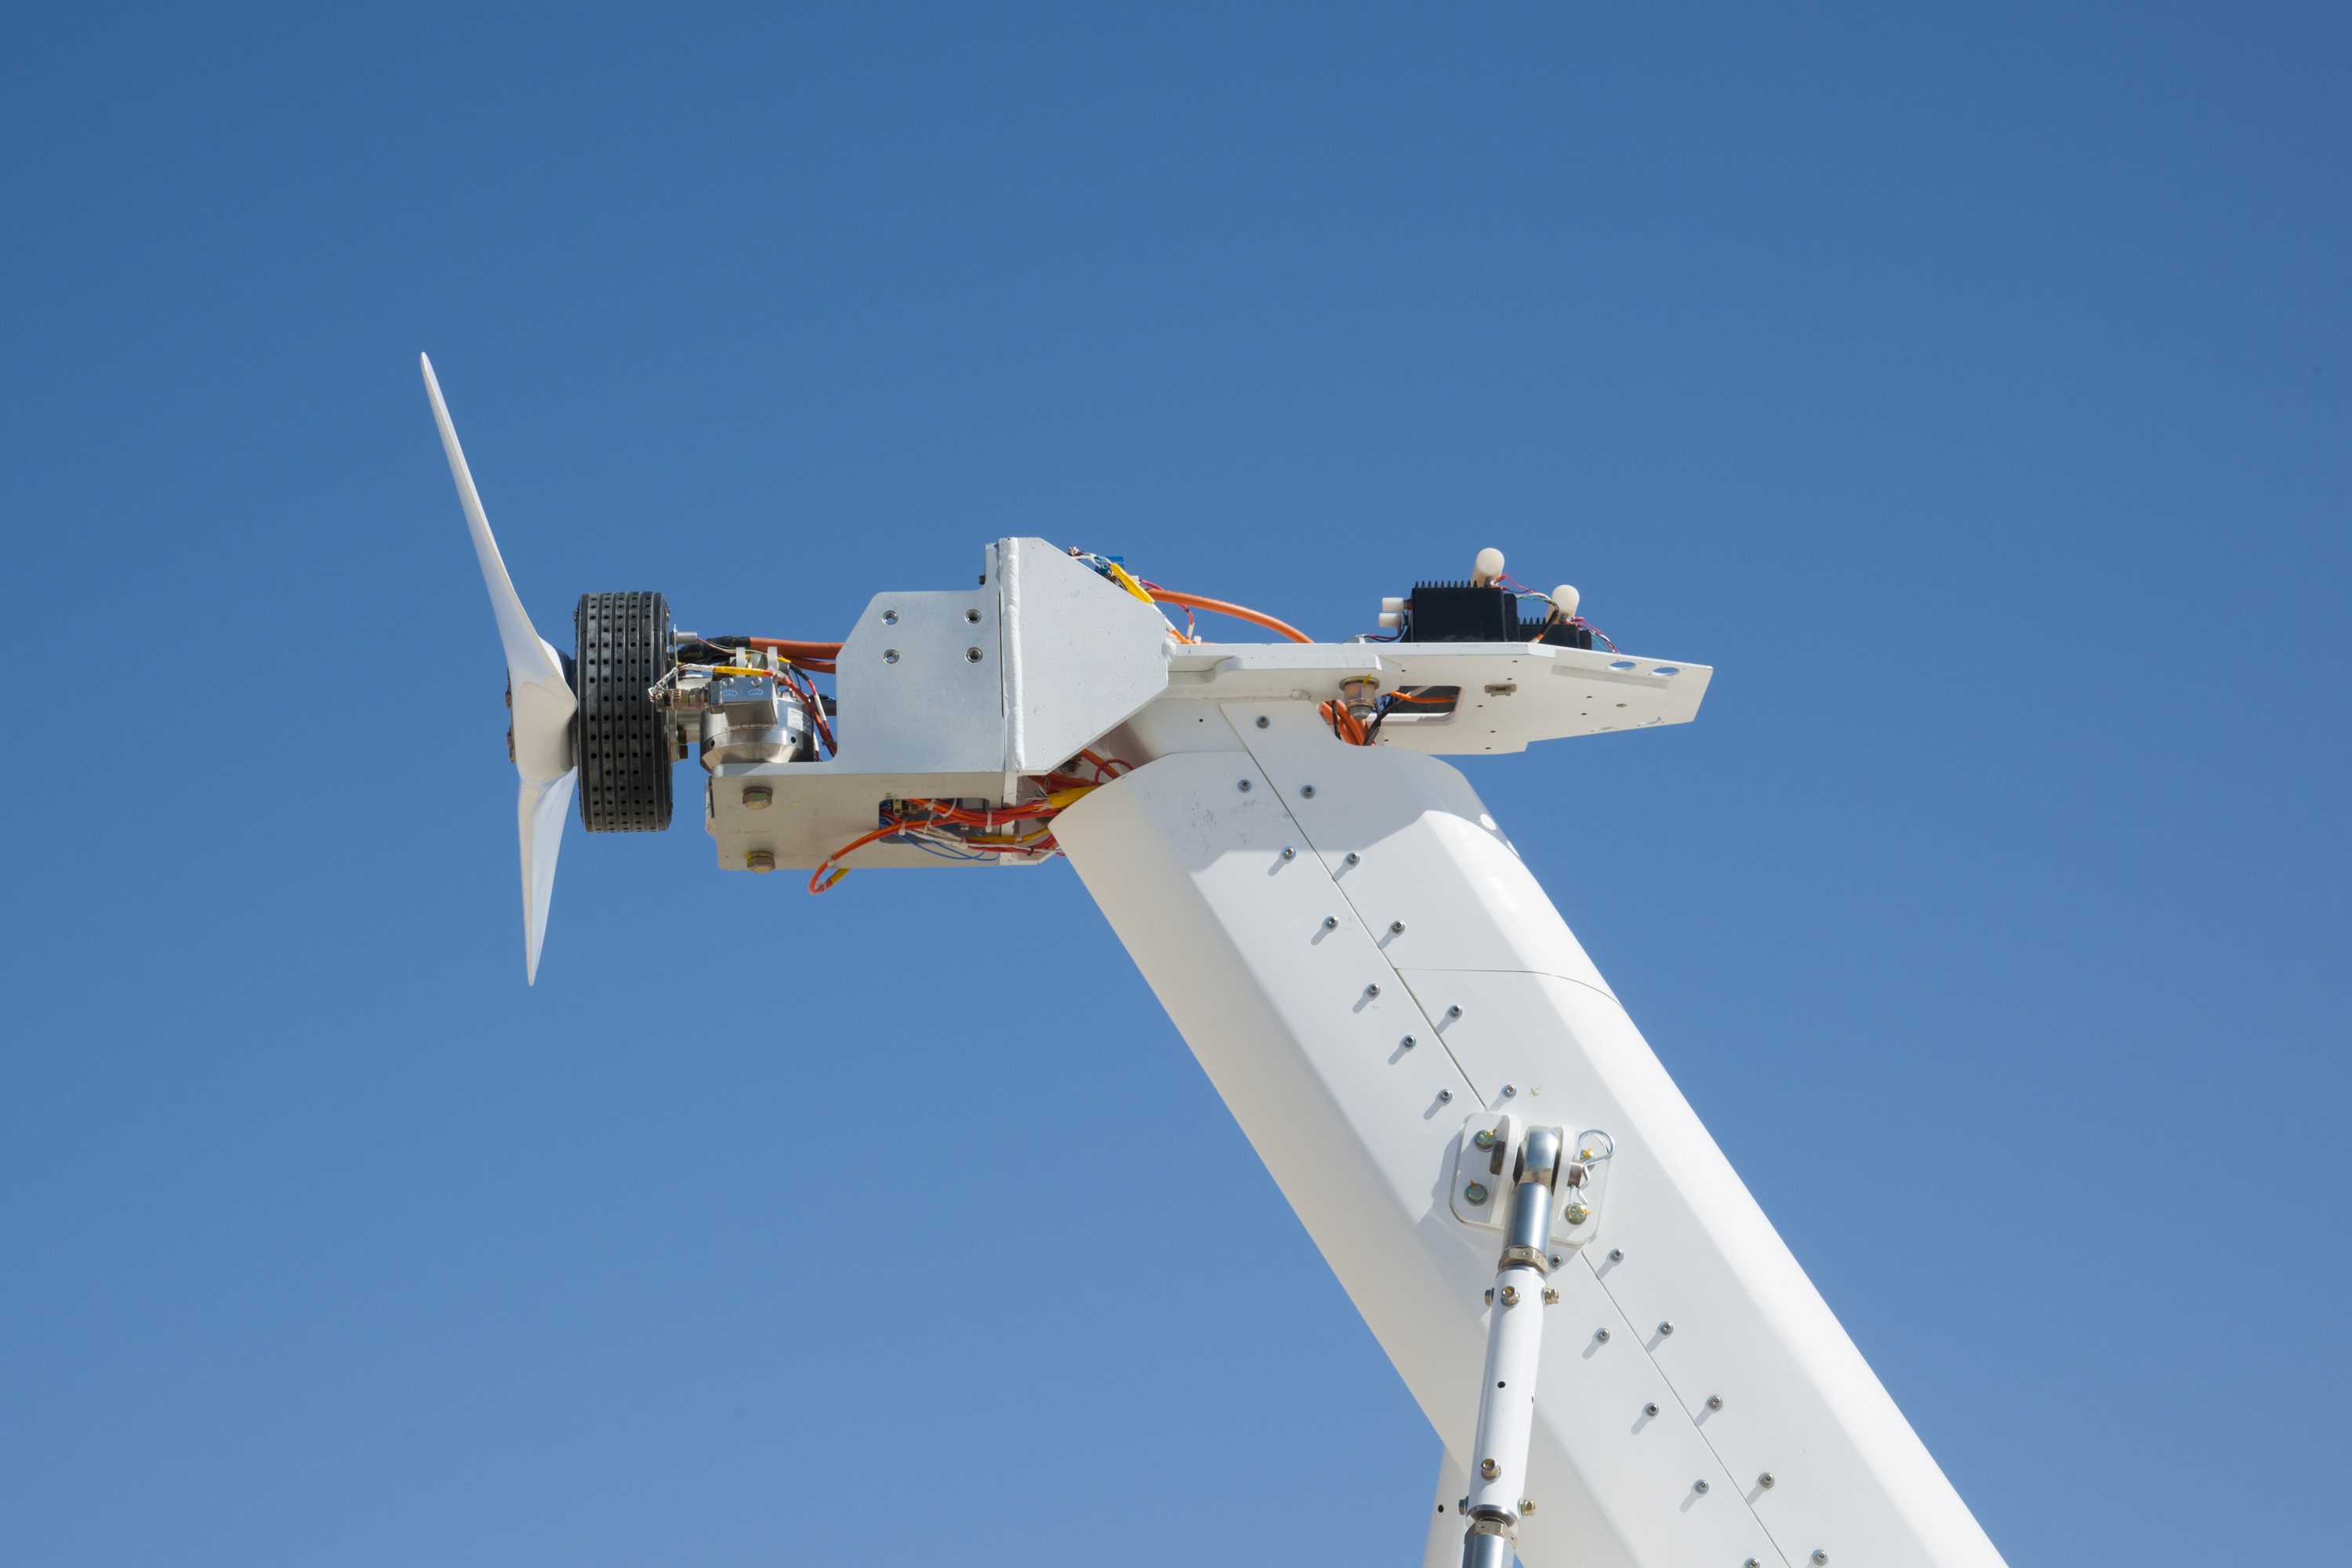
\includegraphics[width=0.85\linewidth,height=\textheight,keepaspectratio]{chapters/02-body/figures/fig02_real_motor_dyno_bench.jpg}

}

\caption{\label{fig-02-real-motor-dyno-bench}\textbf{Instrumented
Electric Motor Dynamometer and Propulsion Test Bench.} An electric motor
undergoing characterization on a dedicated high-bandwidth test stand at
NASA Armstrong Flight Research Center. Direct empirical measurement of
peak torque saturation, electrical time constants (\(\tau_e = L/R\)),
continuous thermal rise (\(\Delta T = P_{\text{loss}} \theta_{JA}\)),
and regenerative power feedback requires synchronizing multi-channel
load cells, optical encoders, isolated current probes, and thermocouple
arrays on a common hardware timebase rather than relying on manufacturer
catalog ratings. (Source: NASA Armstrong Flight Research Center,
Propulsion Systems Laboratory, Public Domain).}

\end{figure}%

Every probe intrudes on the physical process it observes. In software,
instrumentation often introduces context switches, cache eviction, bus
contention, and core heating, altering the execution timing and
scheduling jitter under test. In hardware, attaching a passive voltage
probe adds capacitive loading that distorts high-frequency digital
communication lines, inserting a current shunt in series with a motor
drive drops the rail voltage enough to trigger an early brownout under
load, and placing a thermocouple inside a motor housing alters heat
dissipation paths. On a desktop development platform, motor driver
current sensing uses precision low-side current sense shunts
(\(R_{\text{shunt}} = 10\text{ m}\Omega\text{ to }50\text{ m}\Omega\))
routed to dedicated analog-to-digital converter (ADC) channels on the
real-time microcontroller. Instrument uncertainty is therefore a
compound budget rather than a single tolerance number from a calibration
sheet. It combines sensor linearity, analog-to-digital quantization
error, frequency-dependent phase lag, probe loading effects, and clock
drift between distributed acquisition channels. When an optical encoder
with \(0.05^\circ\) quantization is sampled at \(1000\text{ Hz}\) to
compute joint velocity through discrete backward differences, numerical
differentiation noise introduces velocity variance of several degrees
per second that exists entirely in the measurement pipeline rather than
in the mechanical joint.

A physical limit is meaningless without the complete environmental and
computational context of the machine during the test. Every recorded
limit must state the mechanical payload, ambient temperature, supply
rail voltage, enclosure state, firmware version, and concurrent
computational workload present during the run. An actuator thermal time
constant measured on an open bench at \(20^\circ\text{C}\) with free
convection differs by an order of magnitude from the same actuator
operating inside a sealed composite fairing under direct sunlight at
\(45^\circ\text{C}\). If an electrical characterization omits whether
vision-language model inference was running on the adjacent neural
accelerator during motor stalls, the measured power rail stability
reflects an idle board rather than the combined electrical draw of full
compute and peak actuator torque. Documenting these conditions prevents
engineers from treating a laboratory measurement taken under ideal
cooling and fresh batteries as an absolute physical boundary of the
machine in field deployment.

Systems engineering demands strict discipline in distinguishing measured
physical limits from derived models, manufacturer ratings, and
illustrative figures. Four distinct categories of numbers govern a
machine, comprising direct measurements, derived values, datasheet
ratings, and illustrative examples. Direct measurements are raw,
calibrated time series with specified instruments, sample counts, and
empirical percentiles such as \(P_{50}\), \(P_{99}\), and \(P_{99.9}\).
Derived quantities are computed from direct measurements through
physical models, such as estimating rotor winding temperature from
terminal voltage, phase current across current sense shunts, and an
ambient thermistor trace, which requires propagating the uncertainties
of all three underlying sensors through the thermal model. Datasheet
ratings are nominal manufacturer claims reflecting idealized laboratory
conditions or continuous thermal equilibrium, which rarely hold during
transient impulse loads. Illustrative numbers are analytical examples
used to demonstrate arithmetic or scaling principles in design
calculations, and they must be explicitly labeled as analytical examples
so that no safety margin or architectural timeout relies on them as
measured ground truth.

The absence of a failure during testing establishes a statistical bound
on the failure rate, not an assertion of absolute safety.\sidenote{\footnotesize In
  non-parametric reliability estimation, zero failures across \(n\)
  i.i.d. Bernoulli trials yields the rule-of-three upper bound
  \(p_{\max} \approx 3/n\) at \(95\%\) confidence (exact
  Clopper-Pearson: \(p = 1 - \alpha^{1/n}\)). This bound collapses if
  thermal drift or wear introduces non-stationary confounding.} When an
empirical test of \(n\) independent trials yields zero limit
exceedances, the underlying physical system is not proven to be
defect-free. Let \(p\) represent the true probability of a failure or
limit violation on any single trial. The probability of observing zero
failures across \(n\) independent, identically distributed trials from a
stationary distribution is \((1 - p)^n\). To assert with statistical
confidence \((1 - \alpha)\), such as a \(95\%\) confidence level where
\(\alpha = 0.05\), that the true per-trial failure rate is bounded above
by an upper limit \(p_{\text{max}}\), the observation must satisfy
\((1 - p_{\text{max}})^n \le \alpha\). Taking the natural logarithm of
both sides gives \(n \ln(1 - p_{\text{max}}) \le \ln \alpha\). Applying
the standard linear approximation \(\ln(1 - p) \approx -p\) for small
failure probabilities yields \(-n p_{\text{max}} \le \ln \alpha\), which
simplifies to \(p_{\text{max}} \ge \frac{-\ln \alpha}{n}\). For a
\(95\%\) confidence level where
\(-\ln(0.05) \approx 2.996 \approx 3.0\), the upper bound on the failure
rate is \(p_{\text{max}} \approx \frac{3}{n}\). If an engineer runs
\(n = 3000\) consecutive pick-and-place trajectories on a robotic
manipulator without a brownout or joint collision, this empirical data
supports only the claim that the true per-cycle failure rate is below
\(1.0 \times 10^{-3}\) at \(95\%\) confidence, or roughly one failure
per thousand operations. This derivation holds only when trials are
independent and drawn from a stationary distribution. If motor windings
accumulate heat across successive trials, or if mechanical wear
increases gear backlash over time, consecutive cycles are correlated and
non-stationary. Testing a machine for \(3000\) cycles in a cool morning
laboratory provides zero mathematical guarantee about its failure rate
in the afternoon, when thermal equilibrium increases winding resistance,
lowers peak torque, and shifts the physical system into a brownout
regime.

\protect\phantomsection\label{callout-ruleux2a-2.14}
\begin{fbxSimple}{callout-rule}{Architect’s Rule of Thumb:}{Zero-Failure Statistical Reliability Bound ($p_{\max} \approx 3/n$)}
\phantomsection\label{callout-rule*-2.14}

When an empirical reliability qualification trial of \(n\) independent,
identically distributed operations yields zero limit violations, the
upper bound on the true per-cycle failure probability \(p_{\max}\) at
confidence level \((1 - \alpha)\) is:
\[p_{\max} \approx \frac{-\ln \alpha}{n} \quad \left(p_{\max} \approx \frac{3}{n} \text{ at } 95\%\text{ confidence}\right)\]
This mathematical bound remains valid only while operating conditions
(temperature, battery state of charge, and mechanical wear) remain
strictly stationary across trials.

\end{fbxSimple}

For the physical AI systems engineer, empirical characterization is not
a one-time validation checkbox, but the creation of an immutable
physical contract. Furthermore, this contract must account for
\textbf{lifecycle degradation}: in deployed fleets, physical limits are
non-stationary over operational time. Brake pad friction glazing and
tire tread wear degrade the sustainable deceleration limit
\(a_{\text{brake}}\) by \(15\text{--}30\%\); chemical aging in
lithium-ion battery packs increases internal DC bus impedance
\(R_{\text{bus}}\), exacerbating voltage droop
(\(\Delta V_{\text{droop}}\)) during dynamic maneuvers; and mechanical
gear tooth wear widens backlash clearance \(\delta_{\text{lost}}\).
Every parameter stored in a machine specification---whether a current
ceiling, thermal time constant, or braking deceleration---must record
its physical units, observation points, instrument bandwidth, sample
count, tail percentiles (\(P_{99}\) and \(P_{99.9}\)), and provenance,
with periodic recalibration across the hardware lifecycle. Without this
rigorous physical grounding, safety envelopes remain analytical fictions
that dissolve under the unyielding dynamics of the real world. Yet even
perfectly characterized limits do not remain isolated in operation; on
an integrated machine, physical constraints couple together, creating
compounding stress cascades.

\section{The Cross-Archetype Matrix}\label{sec-body-2-8}

The five physical constraints analyzed across this chapter do not act as
isolated boundaries; they couple together into a unified system
constraint matrix (table~\ref{tbl-02-cross-archetype-matrix}). In
digital computing, software operates under an abstraction of
virtualization: if an inference pass runs late, the user experiences
minor interface lag; if memory is tight, the operating system pages data
to disk. But in an embodied machine, the physical body provides zero
elasticity. When an unconstrained neural policy issues an action
command, that command draws immediate electrical current, generates
non-negotiable kinetic momentum, accelerates reflected rotor inertia,
and dissipates non-reversible Joulean heat into motor stators.

How these physical constraints bind depends directly on the machine's
physical archetype:

\begin{itemize}
\tightlist
\item
  \textbf{Class 1 (Mass-Dominated Mobility):} For autonomous mobile
  robots, automated guided vehicles, and legged platforms,
  \textbf{Momentum and Stopping Distance} is the primary binding limit.
  Kinetic energy grows quadratically with travel speed
  (\(E_{\text{kin}} = \frac{1}{2} m v^2\)), making velocity the master
  multiplier of spatial risk. Sensor age directly expands unguided
  reaction displacement (\(v_0 \Delta t_{\text{delay}}\)), while
  simultaneous multi-axis drive acceleration threatens battery bus
  collapse.
\item
  \textbf{Class 2 (Contact-Dominated Manipulation):} For articulated
  robotic arms, dexterous hands, and automated assembly fixtures,
  \textbf{Actuator Bandwidth, Reflected Rotor Inertia
  (\(N^2 J_{\text{rotor}}\)), and Contact Stiffness} form the primary
  binding envelope. Discontinuous policy setpoints impact rigid fixtures
  with steep force rise rates (\(F = k \Delta x\)), risking gear tooth
  fatigue fracture. Holding heavy payloads against gravity draws
  continuous static stall current, rapidly accumulating thermal stress.
\item
  \textbf{Class 3 (Flow-Dominated Process \& Thermal Plants):} For
  battery energy storage systems, server cooling distribution units, and
  power electronics converters, \textbf{Thermal Dissipation and
  Electrical Power Integrity} govern survival. Long thermal time
  constants (\(\tau = \theta_{JA} C_{\text{th}}\)) hide continuous heat
  accumulation, where a small continuous duty-cycle overload slowly
  drives winding insulation or battery cells into thermal runaway.
\end{itemize}

\begin{longtable}[]{@{}
  >{\raggedright\arraybackslash}p{(\linewidth - 8\tabcolsep) * \real{0.2000}}
  >{\raggedright\arraybackslash}p{(\linewidth - 8\tabcolsep) * \real{0.2000}}
  >{\raggedright\arraybackslash}p{(\linewidth - 8\tabcolsep) * \real{0.2000}}
  >{\raggedright\arraybackslash}p{(\linewidth - 8\tabcolsep) * \real{0.2000}}
  >{\raggedright\arraybackslash}p{(\linewidth - 8\tabcolsep) * \real{0.2000}}@{}}
\caption{\textbf{Cross-Archetype Physical Constraint Matrix.} Systematic
mapping of the five non-negotiable physical constraints to their
governing laws, software illusions, archetype failure modes, and
deterministic systems engineering
takeaways.}\label{tbl-02-cross-archetype-matrix}\tabularnewline
\toprule\noalign{}
\begin{minipage}[b]{\linewidth}\raggedright
Physical Budget / Factor
\end{minipage} & \begin{minipage}[b]{\linewidth}\raggedright
Governing First Principle \& Scaling Law
\end{minipage} & \begin{minipage}[b]{\linewidth}\raggedright
Software Illusion vs.~Hardware Ground Truth
\end{minipage} & \begin{minipage}[b]{\linewidth}\raggedright
Primary Binding Archetype
\end{minipage} & \begin{minipage}[b]{\linewidth}\raggedright
Systems Architect Takeaway \& Runtime Invariant
\end{minipage} \\
\midrule\noalign{}
\endfirsthead
\toprule\noalign{}
\begin{minipage}[b]{\linewidth}\raggedright
Physical Budget / Factor
\end{minipage} & \begin{minipage}[b]{\linewidth}\raggedright
Governing First Principle \& Scaling Law
\end{minipage} & \begin{minipage}[b]{\linewidth}\raggedright
Software Illusion vs.~Hardware Ground Truth
\end{minipage} & \begin{minipage}[b]{\linewidth}\raggedright
Primary Binding Archetype
\end{minipage} & \begin{minipage}[b]{\linewidth}\raggedright
Systems Architect Takeaway \& Runtime Invariant
\end{minipage} \\
\midrule\noalign{}
\endhead
\bottomrule\noalign{}
\endlastfoot
\textbf{1. Measurement Freshness \& Age (§2.2)} &
\(\Delta t_{\text{fresh}} \le \frac{e_{\max}}{v_{\max}}\)\(\Delta t_{\text{e2e}} = \sum_{k=1}^8 \Delta t_k\)
& \emph{Illusion:} High inference rate (\(50\text{ Hz}\)) guarantees
real-time response.\emph{Truth:} Age begins at optical exposure;
pipeline delay adds phase lag (\(-\omega \tau\)). & \textbf{Class 1 \&
2:} Erodes clearance buffer and destabilizes high-gain contact loops. &
Tag frames with hardware timestamps at transduction; check
\(t_{\text{now}} - t_{\text{transduction}} \le \Delta t_{\text{fresh}}\)
at motor registers; reject stale commands. \\
\textbf{2. Momentum \& Stopping Distance (§2.3)} &
\(d_{\text{stop}} = v_0 \Delta t_{\text{delay}} + \frac{v_0^2}{2 a_{\text{brake}}} \le D_{\text{clear}}\)
& \emph{Illusion:} Deceleration can be commanded
instantaneously.\emph{Truth:} Braking distance scales quadratically
(\(v_0^2\)); kinetic energy requires friction work (\(W = F d\)). &
\textbf{Class 1 (Mobility):} Primary constraint. Doubling speed
quadruples braking distance (\(251\%\) total increase). & Solve dynamic
clearance quadratic
\(v_{\max}(D_{\text{clear}}, \Delta t_{\text{delay}})\) at
\(1\text{ kHz}\) in deterministic MCU loop; clamp policy velocity. \\
\textbf{3. Actuator \& Reflected Inertia (§2.4)} &
\(J_{\text{ref}} = N^2 J_{\text{rotor}}\)\(\tau_e = \frac{L}{R}\) ;
\(I(t) \le I_{\max}\) & \emph{Illusion:} Motor torque tracks policy
setpoints without mechanical resistance.\emph{Truth:} Gearbox squares
rotor inertia (\(N^2\)); inductance delays current rise; shock steps
shear teeth. & \textbf{Class 2 (Manipulation):} Primary constraint.
Rigid contacts create extreme \(dF/dt\) force spikes and gear fatigue. &
Enforce \(C^2\) spline (S-curve) trajectory rate limits; sample
load-side optical encoders; deploy quasi-direct drive (QDD)
actuators. \\
\textbf{4. Thermal Limits \& Duty Cycle (§2.5)} &
\(C_{\text{th}} \frac{dT}{dt} = I^2 R(T) - \frac{\Delta T}{\theta_{JA}}\)\(D \le \frac{T_{\max} - T_{\text{amb}}}{P_{\text{peak}} \theta_{JA}}\)
& \emph{Illusion:} Motors deliver peak catalog torque
continuously.\emph{Truth:} Joulean heat (\(I^2 R\)) has positive thermal
feedback (\(\alpha_{\text{Cu}}\)); heat accumulates in sealed housings.
& \textbf{Class 3 (Thermal) \& Class 2:} Static holding draws stall
current, overheating coils in seconds. & Run discrete \(I^2 t\) thermal
observers at \(1\text{ kHz}\) on MCU; dynamically derate speed and
torque when hotspot models approach limits. \\
\textbf{5. Electrical Power Integrity (§2.6)} &
\(\Delta V_{\text{droop}} \approx \Delta I R_{\text{bus}} + \frac{\Delta I \Delta t}{2 C_{\text{bus}}}\)\(V_{\text{final}} = \sqrt{\frac{2(E_{C} + E_{\text{regen}})}{C_{\text{bus}}}}\)
& \emph{Illusion:} Power rails act as infinite, ideal voltage
sources.\emph{Truth:} Bus impedance collapses rail voltage under
combined compute+motor bursts; braking surges overvoltage. &
\textbf{Class 1 \& 3:} Peak multi-axis acceleration trips
microcontroller BOD resets; regen surges destroy inverter FETs. &
Enforce coordinated compute-actuation power budgets and \(dI/dt\)
limits; install dynamic brake choppers; characterize unpowered
fallbacks. \\
\end{longtable}

When an engineer integrates a machine, these five budgets do not fail in
isolation. They form a coupled constraint hypersurface where exceeding a
margin in one domain triggers an immediate failure cascade across
adjacent domains.

\section{Systems Stress-Tests}\label{sec-body-2-9}

To transition from individual physical equations to whole-system
engineering judgment, consider four foundational dilemmas where physical
limits interact across subsystem boundaries to challenge an embodied
machine.

\subsection*{Stress-Test 1: The Thermal-Latency
Avalanche}\label{stress-test-1-the-thermal-latency-avalanche}
\addcontentsline{toc}{subsection}{Stress-Test 1: The Thermal-Latency
Avalanche}

\emph{The scenario.} An autonomous mobile delivery robot operates in a
high-temperature warehouse (\(T_{\text{amb}} = 45^\circ\text{C}\)).
Continuous high-torque maneuvering heats motor windings to
\(110^\circ\text{C}\), elevating the internal chassis air to
\(55^\circ\text{C}\). The onboard neural network accelerator, executing
vision-language navigation policies under heavy compute load, approaches
its \(95^\circ\text{C}\) silicon junction ceiling. This thermal stress
triggers Dynamic Voltage and Frequency Scaling (DVFS), dropping
accelerator clock frequency from \(2.0\text{ GHz}\) to
\(1.3\text{ GHz}\) and inflating inference latency from \(20\text{ ms}\)
to \(31\text{ ms}\).

\emph{The systems dilemma.} Software power managers treat DVFS as an
invisible, transparent background optimization. But on an embodied
machine operating at \(v_0 = 1.5\text{ m/s}\), that \(+11\text{ ms}\)
compute delay injects an unguided reaction displacement of
\(\Delta d_{\text{react}} = 1.65\text{ cm}\). Tracking controllers
expecting \(50\text{ Hz}\) state updates miss deadlines, phase margin
erodes, and the machine exceeds its defended clearance before mechanical
braking can even begin.

\emph{The systems verdict: Coupled Thermal-Timing Invariant.} Actuator
heat dissipation directly inflates computing latency across shared
chassis enclosures. A robust physical AI system must integrate thermal
telemetry with real-time velocity derating, dynamically lowering travel
speed when compute silicon enters thermal throttling.

\subsection*{Stress-Test 2: The Velocity-Clearance-Thermal
Cascade}\label{stress-test-2-the-velocity-clearance-thermal-cascade}
\addcontentsline{toc}{subsection}{Stress-Test 2: The
Velocity-Clearance-Thermal Cascade}

\emph{The scenario.} An automated logistics cart increases its travel
speed from \(v_0 = 1.0\text{ m/s}\) to \(v_0 = 2.0\text{ m/s}\) to meet
warehouse throughput targets, defending a fixed obstacle clearance
\(D_{\text{clear}} = 1.50\text{ m}\) with deceleration limit
\(a_{\text{brake}} = 2.0\text{ m/s}^2\), motor resistance
\(R = 0.8\ \Omega\), and thermal resistance
\(\theta_{JA} = 2.0\text{ K/W}\).

\emph{The systems dilemma.} Doubling travel speed doubles reaction
travel linearly (\(d_{\text{react}} \propto v\)), but quadruples braking
travel quadratically (\(d_{\text{brake}} \propto v^2\)), expanding total
stopping distance from \(0.33\text{ m}\) to \(1.16\text{ m}\) (\(251\%\)
increase) and compressing available clearance buffer from
\(1.17\text{ m}\) down to just \(0.34\text{ m}\). Simultaneously,
high-torque emergency braking demands \(20\text{ A}\) of current,
dumping \(320\text{ W}\) into stator coils (\(4\times\) heating) and
restricting allowable cyclic duty cycle to \(D \le 12.5\%\).

\emph{The systems verdict: Velocity Scaling Law.} Velocity is the master
amplifier of physical risk: it simultaneously expands stopping distance
quadratically, demands peak current against reflected rotor inertia
(\(N^2 J_{\text{rotor}}\)), and accelerates thermal breakdown along
exponential curves.

\subsection*{Stress-Test 3: The Peak-Inference Rail
Collapse}\label{stress-test-3-the-peak-inference-rail-collapse}
\addcontentsline{toc}{subsection}{Stress-Test 3: The Peak-Inference Rail
Collapse}

\emph{The scenario.} A mobile robot powered by a nominal
\(24.0\text{ V}\) lithium-ion battery with internal loop resistance
\(R_{\text{bus}} = 60.0\text{ m}\Omega\) navigates a raised doorway
threshold. A vision transformer inference burst draws \(15.0\text{ A}\)
from the compute rail at the exact millisecond all drive and arm motors
accelerate over the lip, demanding an additional \(55.0\text{ A}\) of
motor current.

\emph{The systems dilemma.} Software assumes compute accelerators and
motor inverters draw from independent, ideal power rails. In reality,
the combined \(70.0\text{ A}\) current transient across
\(R_{\text{bus}} = 60.0\text{ m}\Omega\) induces an instantaneous
voltage droop of \(4.2\text{ V}\). If the battery has partially
discharged to \(21.5\text{ V}\), the bus collapses to \(17.3\text{ V}\),
breaching the \(18.0\text{ V}\) dropout threshold of onboard buck
regulators and triggering a hardware Brownout Detector (BOD) reset on
the real-time microcontroller.

\emph{The systems verdict: Shared Rail Invariant.} Electrical bus
capacity is a shared, instantaneous physical resource. Peak neural
compute bursts coinciding with aggressive mechanical maneuvers can
collapse rail voltages, resetting safety microcontrollers at the exact
instant of maximum kinematic momentum.

\subsection*{Stress-Test 4: The Compound Stress
Protocol}\label{stress-test-4-the-compound-stress-protocol}
\addcontentsline{toc}{subsection}{Stress-Test 4: The Compound Stress
Protocol}

\emph{The scenario.} An engineering team qualifies an articulated robot
arm via two independent bench trials: testing maximum rated payload
(\(15\text{ kg}\)) in a \(20^\circ\text{C}\) laboratory, and testing
empty-gripper trajectory tracking in a \(45^\circ\text{C}\)
environmental chamber. Both isolated tests pass with nominal margins.
The robot is then deployed in a foundry handling maximum payload at
\(45^\circ\text{C}\) with a low battery pack.

\emph{The systems dilemma.} Isolated single-variable testing creates a
false sense of safety. Near battery depletion cutoff, inverters must
draw higher phase current to sustain identical mechanical power
(\(P = V I\)). This elevated current dumps \(I^2 R(T)\) resistive heat
into motor windings whose resistance has already increased by \(47\%\)
due to the \(45^\circ\text{C}\) ambient, driving the arm into
catastrophic thermal shutdown and bus undervoltage within minutes.

\emph{The systems verdict: Compound Qualification Law.} Physical limits
form an interconnected multidimensional hypersurface rather than
independent bounding boxes. Validating an embodied machine requires
subjecting the complete system to simultaneous worst-case thermal,
electrical, and kinematic stress.

\section{Summary}\label{sec-body-2-10}

These five physical limits bound everything built across the system
architecture in Part II. Everything that follows must operate inside the
envelope where mechanics, thermodynamics, and electromagnetism govern
physical hardware. As summarized in the Cross-Archetype Physical
Constraint Matrix (table~\ref{tbl-02-cross-archetype-matrix}), an
engineer cannot negotiate with momentum, dissipate heat faster than
thermal conductance allows, or transport information across a wire
before voltage propagates. The physical body presents five boundaries
that define what the machine can execute without structural damage or
state loss:

\begin{enumerate}
\def\labelenumi{\arabic{enumi}.}
\tightlist
\item
  \textbf{Observation Age:} Sensor signals arrive with non-zero age
  (\(t_{\text{age}}\)), bounded by the physical freshness deadline
  \(\Delta t_{\text{fresh}} \le e_{\max} / v_{\max}\).
\item
  \textbf{Stopping Envelope:} Moving masses sweep through space along an
  unavoidable stopping envelope
  \(d_{\text{stop}} = v_0 \Delta t_{\text{delay}} + \frac{v_0^2}{2 a_{\text{brake}}} \le D_{\text{clear}}\).
\item
  \textbf{Delivered Actuation:} Actuators produce bounded delivered
  torque governed by reflected rotor inertia
  (\(J_{\text{ref}} = N^2 J_{\text{rotor}}\)), winding rise time
  (\(\tau_e = L/R\)), and gear tooth shear limits.
\item
  \textbf{Energy \& Thermal State:} Joulean heat accumulation
  \(P_{\text{loss}} = I^2 R(T)\) under positive thermal feedback
  (\(\alpha_{\text{Cu}}\)) restricts allowable cyclic duty cycles
  (\(D\)).
\item
  \textbf{Electrical Power Integrity:} Shared DC bus impedance droop
  (\(\Delta V_{\text{droop}}\)) and regenerative overvoltage surges
  (\(V_{\text{final}}\)) dictate power delivery stability.
\end{enumerate}

To design a system around these constraints, an engineer must replace
qualitative notions of hardware capacity with exact budgetable
quantities. Observation age is measured as the duration
\(t_{\text{age}}\) from the physical capture of a state change at a
transducer to the moment that measurement updates an internal state
estimate. Stopping envelope is budgeted as the swept physical distance
\(d_{\text{stop}}\) or volume required to bring all kinematic momentum
to zero under maximum braking effort, including sensing delay, brake
engagement latency, and deceleration dynamics. Delivered actuation is
quantified as the usable force, torque, or mechanical bandwidth
delivered at the load interface across joint velocities, bounded by peak
current limits and transmission stiffness. Energy state is budgeted
through two coupled physical mechanisms, specifically the voltage sag
\(\Delta V_{\text{rail}}\) on electrical supply lines under peak motor
transients and the temperature rise \(\Delta T\) across winding
insulation and semiconductor junctions under continuous duty cycles.
Worst-case response time is measured as the tail latency bound,
evaluated at \(P_{99.9}\) or bounded by a deterministic hardware timer,
spanning signal acquisition, transport, compute execution, and actuator
drive update.

Every physical limit is conditional on a declared operating
configuration and loses authority when that configuration changes. A
measured stopping distance or thermal time constant is not a static
property of a component, and it cannot be transferred from a component
datasheet into a safety case without qualification. In an analytical
example of a robotic mobile base carrying a \(50.0\text{ kg}\) payload
at \(2.0\text{ m/s}\), the stopping distance doubles if the payload mass
increases to \(100.0\text{ kg}\) on the same friction surface, or if
surface contaminants reduce the tire traction coefficient by half.
Similarly, a motor winding that operates at a steady-state temperature
of \(75.0^{\circ}\text{C}\) in a \(20.0^{\circ}\text{C}\) laboratory
reaches its thermal destruction threshold if deployed in a
\(45.0^{\circ}\text{C}\) industrial facility under the same duty cycle.
When ambient temperature rises, payload mass increases, supply voltage
drops near battery depletion cutoff, or structural wear degrades
mechanical stiffness, the physical boundaries contract. Operating
outside declared environmental and mechanical baselines invalidates
every timing, force, and energy budget derived from those baselines.

Maintaining integrity across a physical system requires preserving a
complete engineering record for every limit before integrating software
components. That record specifies six mandatory elements for each
boundary. It documents the numerical value or empirical distribution,
such as a \(P_{99.9}\) latency of \(4.2\text{ ms}\) or a maximum
deceleration torque of \(120.0\text{ N}\cdot\text{m}\). It specifies the
exact operating conditions under which that number was established,
including payload, ambient temperature, supply voltage, and surface
properties. It records the measurement uncertainty, identifying the
error bounds of the bench instrumentation used to capture the data. It
allocates a deliberate engineering margin that separates normal
operating targets from absolute physical breakdown thresholds. It
designates a hardware or low-level software detector, such as a
phase-current sensor, optical interrupter, or supply-rail voltage
monitor, responsible for catching boundary excursions in real time. It
records provenance, distinguishing whether a bound is derived from
analytical mechanics or measured directly on physical hardware under
stress.

\protect\phantomsection\label{callout-takeawaysux2a-2.15}
\begin{fbxSimple}{callout-takeaways}{Key Chapter Takeaways}{}
\phantomsection\label{callout-takeaways*-2.15}

\begin{itemize}
\tightlist
\item
  \textbf{Freshness is Measured at Transduction:} Observation age begins
  at photon capture on sensor silicon, not at model inference. Carry
  hardware timestamps to the motor register boundary and reject stale
  commands
  (\(t_{\text{now}} - t_{\text{transduction}} \le \Delta t_{\text{fresh}}\)).
\item
  \textbf{Velocity is the Master Risk Multiplier:} Travel speed scales
  reaction travel linearly (\(d_{\text{react}} \propto v\)), braking
  distance quadratically (\(d_{\text{brake}} \propto v^2\)), and stator
  heat dissipation quadratically (\(I^2 R\)).
\item
  \textbf{Gearboxes Reflect Rotor Inertia Quadratically:} Gear ratio
  \(N\) multiplies rotor inertia by \(N^2\), turning rapid motor
  acceleration into violent mechanical shock unless filtered with
  \(C^2\) continuous splines.
\item
  \textbf{Thermal Heat Accumulates Silently:} Joulean dissipation
  (\(I^2 R\)) creates positive thermal feedback
  (\(\alpha_{\text{Cu}}\)). Enforce cyclic duty cycles (\(D\)) and
  real-time \(I^2 t\) thermal observers.
\item
  \textbf{Electrical Power is a Shared Resource:} Simultaneous compute
  and motor acceleration transients collapse DC bus voltages, triggering
  brownout resets at the moment of peak kinematic momentum.
\item
  \textbf{Tail Distributions Rule Physical Safety:} Physical safety is
  governed by tail percentiles (\(P_{99.9}\)) and zero-failure
  statistical bounds (\(p_{\max} \approx 3/n\)), not by median bench
  performance.
\end{itemize}

\end{fbxSimple}

\textbf{?@sec-brain} takes custody of this constrained physical body and
addresses the machine from the inside out. With physical envelopes
established, the engineering objective is not to modify the physical
laws that govern the machine, but to build a nervous system and a
learned brain that respect them under all operating conditions. A neural
network policy possesses high representational capacity, but it has no
innate awareness of winding temperatures, bus saturation, or stopping
distances. The nervous system must enforce these five limits
deterministically, providing the safety and timing guarantees that the
learned model cannot provide for itself. The chapters ahead examine what
a learned component contributes to physical autonomy once its authority
is bounded within these measured physical limits.

\protect\phantomsection\label{refs}
\begin{CSLReferences}{1}{1}
\bibitem[\citeproctext]{ref-lynch2017modern}
Lynch, Kevin M, and Frank C Park. 2017. \emph{Modern Robotics:
Mechanics, Planning, and Control}. Cambridge University Press.

\bibitem[\citeproctext]{ref-maxwell1868governors}
Maxwell, J Clerk. 1868. {``On Governors.''} \emph{Proceedings of the
Royal Society of London} 16: 270--83.

\bibitem[\citeproctext]{ref-nasa1999mco}
NASA Mishap Investigation Board. 1999. \emph{Mars Climate Orbiter Mishap
Investigation Board Phase i Report}. National Aeronautics; Space
Administration.

\bibitem[\citeproctext]{ref-ntsb2019uber}
National Transportation Safety Board. 2019. \emph{Collision Between a
Self-Driving Car and a Pedestrian, Tempe, Arizona, March 18, 2018}.
HAR-19/03. NTSB.

\end{CSLReferences}


\backmatter


\end{document}
